\documentclass[a4paper, 12pt, oneside]{article}

%% ─────────────────────────────────────────
%%  MSc Thesis, Cranfield University / ESTIA
%%  Preamble inherited from the ALTEN BST (docs/BST_DISCO_JH_2026/main.tex)
%%  so that both documents share one visual identity.
%% ─────────────────────────────────────────

%% ─────────────────────────────────────────
%%  ENCODING & FONTS
%% ─────────────────────────────────────────
\usepackage[utf8]{inputenc}
\usepackage[T1]{fontenc}
\usepackage{microtype}

%% ALTEN Brandbook 2025 — main font is Metropolis; in its absence the
%% brand prescribes Arial or Calibri. Carlito is the metric-compatible
%% free Calibri, so the whole document is set in it.
\usepackage[sfdefault,lining]{carlito}

%% ─────────────────────────────────────────
%%  ALTEN BRAND COLOURS (Brandbook EN, Sept. 2025)
%% ─────────────────────────────────────────
\usepackage{xcolor}
% Main trio
\definecolor{altenAzure}{HTML}{008BD2}   % Azure blue
\definecolor{altenNavy}{HTML}{043962}    % Navy blue — running text colour
\definecolor{altenOchre}{HTML}{FFDA65}   % Ochre yellow
% Official shades
\definecolor{altenAzureDark}{HTML}{176F98}
\definecolor{altenAzureLight}{HTML}{7DCAED}
\definecolor{altenAzurePale}{HTML}{B2E0F5}
\definecolor{altenNavyShade}{HTML}{4A617D}
\definecolor{altenOchreDark}{HTML}{FFBA00}
\definecolor{altenOchrePale}{HTML}{FFEF86}
% Greyscale / bluescale (backgrounds, lines, secondary text)
\definecolor{altenGreyBg}{HTML}{EBECF0}
\definecolor{altenGreyLine}{HTML}{CDCEDA}
\definecolor{altenGreyText}{HTML}{8C8C9A}
\definecolor{altenBlueBg}{HTML}{EBF3F9}
\definecolor{altenBlueBg2}{HTML}{DAE8F3}
\definecolor{altenBlueBg3}{HTML}{CBEAF8}

%% Coloured section headings (azure titles on navy text, per charter)
\usepackage{sectsty}
\sectionfont{\color{altenNavy}}
\subsectionfont{\color{altenAzureDark}}
\subsubsectionfont{\color{altenAzureDark}}
\paragraphfont{\color{altenNavy}}

%% ─────────────────────────────────────────
%%  PAGE GEOMETRY
%%  article defaults leave very wide margins on A4 at 12pt, which pushes
%%  wide tables into overfull boxes and inflates the page count.
%% ─────────────────────────────────────────
\usepackage[a4paper, top=2.6cm, bottom=2.6cm, left=2.7cm, right=2.7cm,
            footskip=1.1cm]{geometry}

%% Derniere reserve avant qu'une ligne ne parte dans la marge.
\setlength{\emergencystretch}{2em}

%% ─────────────────────────────────────────
%%  FLOAT PLACEMENT
%%  Allow a float to take more of a page and require less text on a mixed
%%  page, so figures stop generating half-empty pages.
%% ─────────────────────────────────────────
\renewcommand{\topfraction}{0.9}
\renewcommand{\bottomfraction}{0.7}
\renewcommand{\textfraction}{0.12}
\renewcommand{\floatpagefraction}{0.75}
\setcounter{topnumber}{3}
\setcounter{bottomnumber}{2}
\setcounter{totalnumber}{4}

%% ─────────────────────────────────────────
%%  PAGE STYLE
%% ─────────────────────────────────────────
\pagestyle{plain}

\usepackage{fancyhdr}
\fancypagestyle{plain}{
    \fancyhf{}
    \fancyfoot[R]{\ShortTitle\\\textbf{Company Confidential}}
    \fancyfoot[L]{Cranfield University\\MSc CSTE 2025--2026}
    \renewcommand{\headrulewidth}{0pt}
    \renewcommand{\footrulewidth}{1pt}
}

%% ─────────────────────────────────────────
%%  PARAGRAPH LAYOUT — uniform spacing, no indents
%% ─────────────────────────────────────────
\usepackage[skip=8pt plus 2pt, indent=0pt]{parskip}

%% ─────────────────────────────────────────
%%  TOC DEPTH
%% ─────────────────────────────────────────
\setcounter{tocdepth}{3}
\setcounter{secnumdepth}{3}

%% ─────────────────────────────────────────
%%  BIBLIOGRAPHY — biblatex ISO-690
%%  The BST bibliography is referenced, never modified; thesis-only
%%  citations live in a second resource.
%% ─────────────────────────────────────────
\usepackage[
    style       = iso-authoryear,
    backend     = biber,
    sorting     = nyt,
    maxbibnames = 3,
    minbibnames = 1,
    giveninits  = true,
    urldate     = iso,
]{biblatex}
\addbibresource{../BST_DISCO_JH_2026/Utilities/Bibliography.bib}
\addbibresource{Utilities/Bibliography_thesis.bib}
\usepackage[nottoc,numbib]{tocbibind}

%% ─────────────────────────────────────────
%%  GLOSSARY — shared with the BST
%% ─────────────────────────────────────────
\usepackage[acronym, section=subsection]{glossaries}
\makenoidxglossaries{}
%% ─────────────────────────────────────────────────────────────────────────
%%  ACRONYMS
%% ─────────────────────────────────────────────────────────────────────────
\newacronym{ahp}{AHP}{Analytic Hierarchy Process}
\newacronym{bst}{BST}{Bilan Scientifique et Technique}
\newacronym{bwm}{BWM}{Best-Worst Method}
\newacronym{ci}{CI}{Consistency Index}
\newacronym{cr}{CR}{Consistency Ratio}
\newacronym{csrd}{CSRD}{Corporate Sustainability Reporting Directive}
\newacronym{dag}{DAG}{Directed Acyclic Graph}
\newacronym{din}{DIN}{Direction Innovation Num\'erique}
\newacronym{disco}{DISCO}{Supply Chain Illustrator (Digital Twin, DIN ALTEN)}
\newacronym{dt}{DT}{Digital Twin}
\newacronym{fbwm}{F-BWM}{Fuzzy Best-Worst Method}
\newacronym{glec}{GLEC}{Global Logistics Emissions Council}
\newacronym{hgv}{HGV}{Heavy Goods Vehicle}
\newacronym{iot}{IoT}{Internet of Things}
\newacronym{ipg}{IPG}{Itinerary Performance Index}
\newacronym{kpi}{KPI}{Key Performance Indicator}
\newacronym{lppl}{LPPL}{Log-Periodic Power Law}
\newacronym{mcdm}{MCDM}{Multi-Criteria Decision-Making}
\newacronym{mts}{MTS}{Manchester Triage System}
\newacronym{pi}{PI}{Physical Internet}
\newacronym{promethee}{PROMETHEE}{Preference Ranking Organisation METHod for Enrichment Evaluation}
\newacronym{ri}{RI}{Random Index (Saaty)}
\newacronym{sc}{SC}{Supply Chain}
\newacronym{tmt}{TMT}{Temporal Motivational Theory}
\newacronym{tfn}{TFN}{Triangular Fuzzy Number}
\newacronym{tts}{TTS}{Time To Service}
\newacronym{ttr}{TTR}{Time To Recovery}
\newacronym{vecto}{VECTO}{Vehicle Energy Consumption calculation TOol}
\newacronym{xai}{XAI}{Explainable Artificial Intelligence}

%% ─────────────────────────────────────────────────────────────────────────
%%  MAIN GLOSSARY ENTRIES (key mathematical symbols and concepts)
%% ─────────────────────────────────────────────────────────────────────────
\newglossaryentry{ur}{
    name={$U_r(t)$},
    description={Real (operationally computable) urgency at time $t$: a
        weighted probabilistic OR aggregation of six local KPI blocks
        (time, capacity, performance, risk, cost, CO2), $U_{r,\text{local}}
        = 1-\prod_m(1-u_m)^{\omega_m}$, propagated upstream across the
        supply chain DAG through the leaky coefficients $\beta_{ji}$}}

\newglossaryentry{ud}{
    name={$U_d$},
    description={Declared urgency, a scalar $\in [0,1]$ elicited from the
        human operator via an AHP or Fuzzy-BWM questionnaire, propagated
        downstream across the supply chain DAG through the leaky
        coefficients $\gamma_{ik}$}}

\newglossaryentry{at}{
    name={$A(t)$},
    description={Adequacy score at time $t$, quantifying the asymmetric
        Prospect Theory penalty between $U_d$ and $U_r(t)$:
        $A = 100\times(\exp(-\text{penalty})-\text{floor})/(1-\text{floor})$
        with $\text{penalty}=\lambda_{\text{under}}H^{\alpha}+
        \lambda_{\text{over}}F^{\alpha}$, $\in [0,100]$}}

\newglossaryentry{deltau}{
    name={$\Delta U(t)$},
    description={Raw urgency mismatch: $U_d - U_r(t) \in (-1,1)$; positive
        = over-triage (false urgency), negative = under-triage
        (hidden risk)}}

\newglossaryentry{fh}{
    name={$F$, $H$},
    description={False urgency $F=[U_d-U_r]_+$ (unjustified panic) and
        hidden risk $H=[U_r-U_d]_+$ (silent danger), the two asymmetrically
        penalised pathologies underlying $A(t)$}}

\newglossaryentry{omegam}{
    name={$\omega_m$},
    description={Aggregation weight of KPI block $m$ in the real urgency
        noisy-OR aggregation, reused unchanged as the PROMETHEE~II
        criteria weight for network-wide node outranking}}

\newglossaryentry{deltaurcrit}{
    name={$\Delta U_{r,\text{final}}$},
    description={Network criticality delta: the increase in real urgency
        propagated to final-customer nodes when a given node's local
        urgency is forced to saturation in a systematic shock simulation}}


%% ─────────────────────────────────────────
%%  SCHEMAS VECTORIELS
%%  Une figure conceptuelle est dessinee plutot que capturee : elle reste
%%  nette a l'impression et suit la charte du document.
%% ─────────────────────────────────────────
\usepackage{tikz}
\usetikzlibrary{arrows.meta, positioning, calc, fit, backgrounds, shapes.geometric,
                decorations.pathreplacing}

%% Une boite de schema ne se coupe jamais en fin de ligne : un mot coupe dans
%% un encadre de trois centimetres se lit deux fois moins vite.
\newcommand{\SansCesure}{\hyphenpenalty=10000\exhyphenpenalty=10000\relax}

\tikzset{
  %% ── Boxes ────────────────────────────────────────────────────────────
  %% Three weights, and they have to be distinguishable at print size: a
  %% strong box is the subject, a plain box is the mechanism, a pale box is
  %% context the reader may skip.
  bloc/.style       = {draw=altenNavy, line width=0.85pt, rounded corners=3pt,
                       fill=altenBlueBg, text=altenNavy, align=center,
                       inner sep=4pt, font=\scriptsize,
                       execute at begin node=\SansCesure},
  blocFort/.style   = {bloc, fill=altenAzure!26, draw=altenAzure,
                       line width=1.15pt},
  blocPale/.style   = {bloc, fill=altenGreyBg!55!white, draw=altenGreyLine,
                       text=altenNavyShade, line width=0.75pt},
  blocObs/.style    = {bloc, fill=altenOchrePale!70!white, draw=altenOchreDark,
                       line width=1.15pt},
  blocAlerte/.style = {bloc, fill=altenOchrePale!70!white, draw=altenOchreDark,
                       line width=1.15pt},
  %%
  %% ── Arrows ───────────────────────────────────────────────────────────
  %% Direction is the content of most of these diagrams, so the heads are
  %% sized to survive printing rather than to look delicate on screen.
  fleche/.style     = {-{Stealth[length=2.8mm, width=2.0mm]}, draw=altenNavy,
                       line width=0.85pt},
  flecheCoupee/.style = {-{Stealth[length=2.8mm, width=2.0mm]},
                       draw=altenOchreDark, line width=1.0pt,
                       dash pattern=on 2.2pt off 1.8pt},
  flecheObs/.style  = {-{Stealth[length=2.8mm, width=2.0mm]},
                       draw=altenOchreDark, line width=1.1pt},
  flechePale/.style = {-{Stealth[length=2.6mm, width=1.8mm]},
                       draw=altenGreyLine, line width=0.75pt},
  %%
  %% ── Text ─────────────────────────────────────────────────────────────
  %% A label sits on top of arrows and rules, so it carries an opaque fill;
  %% a column title sits above the diagram and does not.
  etiquette/.style  = {font=\scriptsize\itshape, text=altenAzureDark,
                       inner sep=2.5pt, fill=white, align=center,
                       execute at begin node=\SansCesure},
  titreBande/.style = {font=\small\bfseries, text=altenNavy, align=left},
}

%% ─────────────────────────────────────────
%%  MATHEMATICS
%% ─────────────────────────────────────────
\usepackage{amsmath, amssymb, mathtools}
\usepackage{amsthm}

%% Enonces formels : une proposition se demontre, une hypothese de modele se
%% discute. Les deux styles sont distincts pour que le lecteur sache lequel
%% il lit avant d'en lire le contenu.
\newtheoremstyle{alten}{9pt}{9pt}{}{0pt}{\bfseries\color{altenNavy}}{.}{.5em}{}
\theoremstyle{alten}
\newtheorem{proposition}{Proposition}[section]
\newtheorem{assumption}{Assumption}[section]
\newtheorem{definition}{Definition}[section]
\renewcommand{\qedsymbol}{\color{altenAzure}$\blacksquare$}

%% ─────────────────────────────────────────
%%  ALGORITHMS
%%  Le coeur du systeme est une recurrence sur un DAG. La prose la decrit ;
%%  seul le pseudo-code la rend verifiable et chiffrable en complexite.
%% ─────────────────────────────────────────
\usepackage{algorithm}
\usepackage{algpseudocode}
\floatname{algorithm}{Algorithm}
\renewcommand{\algorithmicrequire}{\textbf{\color{altenNavy}Input:}}
\renewcommand{\algorithmicensure}{\textbf{\color{altenNavy}Output:}}
\algrenewcommand\algorithmicfor{\textbf{\color{altenAzureDark}for}}
\algrenewcommand\algorithmicwhile{\textbf{\color{altenAzureDark}while}}
\algrenewcommand\algorithmicif{\textbf{\color{altenAzureDark}if}}
\algrenewcommand\algorithmicelse{\textbf{\color{altenAzureDark}else}}
\algrenewcommand\algorithmicend{\textbf{\color{altenAzureDark}end}}
\algrenewcommand\algorithmicreturn{\textbf{\color{altenAzureDark}return}}
\algrenewcommand\algorithmicdo{\textbf{\color{altenAzureDark}do}}
\algrenewcommand\algorithmicthen{\textbf{\color{altenAzureDark}then}}
\algnewcommand{\LineComment}[1]{\State \(\triangleright\) \textit{\color{altenGreyText}#1}}
%% Une ligne d'algorithme trop longue doit rester lisible : corps en small.
\makeatletter
\renewcommand{\ALG@beginalgorithmic}{\small}
\makeatother



%% ─────────────────────────────────────────
%%  MEDIA / GRAPHICS
%%  Figures come from the BST image tree and from this document's own tree.
%% ─────────────────────────────────────────
\usepackage{rotating}
\usepackage{graphicx}
\graphicspath{{./}{../BST_DISCO_JH_2026/}}
\usepackage{caption}
%% Un DOI n'offre aucun point de coupure naturel : sans xurl la
%% bibliographie deborde dans la marge sur une page sur deux.
\usepackage{xurl}
\usepackage[hidelinks]{hyperref}

%% ─────────────────────────────────────────
%%  TABLES
%%  Rules and captions carry the navy body colour, so a table does not
%%  read as a black island in a navy document.
%% ─────────────────────────────────────────
\usepackage{tabularx, array, booktabs, multirow, longtable, float}
\usepackage{colortbl}  % provides \arrayrulecolor
%% Colonne X alignee en haut comme les colonnes p : centrer verticalement
%% la seule colonne elastique desalignait chaque ligne du tableau.
\renewcommand{\tabularxcolumn}[1]{p{#1}}
\arrayrulecolor{altenNavy}

%% Captions: navy label, navy text, matching the running colour
\captionsetup{labelfont={bf,color=altenNavy}, textfont={color=altenNavy},
              font=small}

%% ─────────────────────────────────────────
%%  LISTS
%% ─────────────────────────────────────────
\usepackage{enumitem}
\setitemize{parsep=0pt, partopsep=0pt}
\setenumerate{parsep=0pt, partopsep=0pt}

%% ─────────────────────────────────────────
%%  HYPERLINKS
%% ─────────────────────────────────────────
\hypersetup{
    colorlinks  = true,
    linkcolor   = altenAzure,
    filecolor   = altenAzure,
    urlcolor    = altenAzure,
    citecolor   = altenAzure,
    pdftitle    = {Measuring and Closing the Gap Between Declared and Real Urgency in a Supply Chain Digital Twin},
    pdfauthor   = {John Hoarau},
}

%% ─────────────────────────────────────────
%%  TOC SPACING
%% ─────────────────────────────────────────
\makeatletter
\pretocmd{\section}{\addtocontents{toc}{\protect\addvspace{5\p@}}}{}{}
\pretocmd{\subsection}{\addtocontents{toc}{\protect\addvspace{5\p@}}}{}{}
\pretocmd{\subsubsection}{\addtocontents{toc}{\protect\addvspace{5\p@}}}{}{}
\makeatother

%% ─────────────────────────────────────────
%%  COLOURED BOXES
%% ─────────────────────────────────────────
\usepackage[strict]{changepage}
\usepackage{framed}

\colorlet{definitionshade}{altenBlueBg2}
\newenvironment{definitionBox}{%
  \def\FrameCommand{%
    \hspace{1pt}%
    {\color{altenNavy}\vrule width 2pt}%
    {\color{definitionshade}\vrule width 4pt}%
    \colorbox{definitionshade}%
  }%
  \MakeFramed{\advance\hsize-\width\FrameRestore}%
  \noindent\hspace{-4.55pt}%
  \begin{adjustwidth}{}{7pt}%
  \vspace{2pt}\vspace{2pt}%
}{\vspace{2pt}\end{adjustwidth}\endMakeFramed}

\colorlet{exampleShade}{altenBlueBg}
\newenvironment{exampleBox}{%
  \def\FrameCommand{%
    \hspace{1pt}%
    {\color{altenAzure}\vrule width 2pt}%
    {\color{exampleShade}\vrule width 4pt}%
    \colorbox{exampleShade}%
  }%
  \MakeFramed{\advance\hsize-\width\FrameRestore}%
  \noindent\hspace{-4.55pt}%
  \begin{adjustwidth}{}{7pt}%
  \vspace{2pt}\vspace{2pt}%
}{\vspace{2pt}\end{adjustwidth}\endMakeFramed}

%% Brand charter excludes red: attention accents use ochre yellow instead
\colorlet{attentionShade}{altenOchrePale!45!white}
\newenvironment{attentionBox}{%
  \def\FrameCommand{%
    \hspace{1pt}%
    {\color{altenOchreDark}\vrule width 2pt}%
    {\color{attentionShade}\vrule width 4pt}%
    \colorbox{attentionShade}%
  }%
  \MakeFramed{\advance\hsize-\width\FrameRestore}%
  \noindent\hspace{-4.55pt}%
  \begin{adjustwidth}{}{7pt}%
  \vspace{2pt}\vspace{2pt}%
}{\vspace{2pt}\end{adjustwidth}\endMakeFramed}

%% ─────────────────────────────────────────
%%  COMMENTS
%% ─────────────────────────────────────────
\usepackage{comment}

%%%%%%%%%%%%%%%%%%%%%%%%%%%%%%%%%%%%%%%%%%%%%%%%%%%%%%%%%%%
%% BEGIN OF DOCUMENT
%%%%%%%%%%%%%%%%%%%%%%%%%%%%%%%%%%%%%%%%%%%%%%%%%%%%%%%%%%%

\begin{document}

%% ALTEN charter: running text is navy blue, never black
\color{altenNavy}

\newcommand{\ShortTitle}{Declared vs.\ Real Urgency: MSc Thesis 2026}

%% Four logos: the awarding university and the delivering school at the top, the
%% industrial partners at the bottom. Spacing is deliberately tight and explicit,
%% because the whole block must fit on one A4 page. If a logo height is changed,
%% the vertical spaces below must be rebalanced or the footer spills to page 2.
%% Cranfield and ESTIA marks are the trimmed copies in Images/0.Cover of this
%% project; ALTEN and DIN resolve from the BST image tree through \graphicspath.
\begin{titlepage}
    \centering

    \noindent
    \begin{minipage}[c]{0.46\textwidth}
        \centering
        
\includegraphics[height=1.85cm, keepaspectratio]{Images/0.Cover/LogoCranfield.png}
    \end{minipage}\hfill
    \begin{minipage}[c]{0.46\textwidth}
        \centering
        
\includegraphics[height=1.00cm, keepaspectratio]{Images/0.Cover/LogoESTIA.png}
    \end{minipage}

    \vspace{0.62cm}

    {\large JOHN HOARAU\par}

    \vspace{0.38cm}

    {\Large\bfseries
        Measuring and Closing the Gap Between\\[3pt]
        Declared and Real Urgency in a\\[3pt]
        Supply Chain Digital Twin\par}

    \vspace{0.22cm}
    {\small\itshape Cognitive adequacy scoring, forecast-assisted declaration,\\
        and an opening towards satellite-observed capacity\par}

    \vspace{0.36cm}

    {\small
        Engineering and Applied Sciences\par
        Thesis\par}

    \vspace{0.20cm}

    {\small
        MSc in Computational and Software Techniques in Engineering\par
        Digital Engineering Design\par
        ESTIA Institute of Technology, Bidart\par}

    \vspace{0.16cm}
    {\small Academic Year: 2025--2026\par}

    \vspace{0.32cm}

    {\small
        \begin{tabular}{@{}r@{\hspace{0.8em}}l@{}}
        Academic Supervisor (Cranfield): & Dr Peter Sherar \\[1pt]
        Academic Supervisor (ESTIA):     & Prof.\ David Gomez \\[1pt]
        Industrial Supervisor:           & S\'ebastien Perthuisot, ALTEN-DIN \\
        \end{tabular}\par}

    \vspace{0.30cm}
    {\small August 2026\par}

    \vspace{0.30cm}

    \noindent
    \begin{minipage}[c]{.5\textwidth}
        \centering
        
\includegraphics[height=1.05cm, keepaspectratio]{Images/0.Cover/LogoALTEN.png}
    \end{minipage}%
    \begin{minipage}[c]{.5\textwidth}
        \centering
        
\includegraphics[height=1.05cm, keepaspectratio]{Images/0.Cover/LogoDIN.png}
    \end{minipage}

    \vspace{0.18cm}

    {\footnotesize
        Research carried out at the Direction Innovation Num\'erique, ALTEN Group\par}

    \vspace{0.06cm}
    {\footnotesize
        \textcopyright{} Cranfield University 2026. All rights reserved. No part of
        this publication\par
        may be reproduced without the written permission of the copyright
        owner.\par}

    \vspace{0.14cm}
    {\footnotesize\bfseries Company Confidential\par}

\end{titlepage}


\clearpage
\pagenumbering{roman}
\section*{Declarations}
\label{sec:declaration}
\addcontentsline{toc}{section}{Declarations}

\subsection*{Academic integrity}

I declare that:

\begin{itemize}[leftmargin=1.4em, itemsep=2pt]
    \item the thesis submitted has been written by me alone;
    \item the thesis submitted has not been previously submitted to this
          university or any other;
    \item all content, including primary and secondary data, is true to the best
          of my knowledge;
    \item all quotations and references have been duly acknowledged according to
          the requirements of academic research.
\end{itemize}

I understand that to knowingly submit work in violation of the above statement
will be considered by examiners as academic misconduct.

\subsection*{Confidentiality}

This thesis contains commercially sensitive information belonging to the ALTEN
Group, including internal scoring parameters and the architecture of an
unreleased software product. It is submitted for examination on a confidential
basis and is marked \emph{Company Confidential} throughout.

\subsection*{Use of software tools}

Numerical results were produced with the Python codebase described in
Section~\ref{sec:methods_impl}, using NumPy, SciPy, Matplotlib, Shapely, PyProj
and Ultralytics. Large language models were used in two distinct and clearly
separated capacities. First, as an \emph{object of study}: the declarants of both
campaigns are language models, an experimental design choice reported and
discussed as such in Sections~\ref{sec:methods_arms} and~\ref{sec:res_armB}.
Second, as a \emph{writing aid} for language correction and \LaTeX{} formatting.
All scientific claims, all numerical results and all interpretations are my own,
and every figure in this thesis was produced either by the project's own code or
drawn by hand.


\clearpage
\section*{Abstract}
\label{sec:abstract}
\addcontentsline{toc}{section}{Abstract}
In mutualised logistics networks the urgency an operator declares often diverges from the
urgency computable from the operational state. Over-declaration wastes shared capacity;
under-declaration hides rupture risk. No existing digital twin measures that divergence or
propagates it across a supplier network.

This thesis builds and tests one. Real urgency is aggregated at each node from six KPI blocks
through a weighted probabilistic OR and propagated upstream across a directed acyclic supply
graph; declared urgency is elicited through a consistency-gated pairwise questionnaire and
propagated downstream; their mismatch is scored on $[0,100]$ with an asymmetric
Prospect-Theory penalty. The system was evaluated through a pre-registered campaign replaying
the 2020 to 2022 semiconductor shortage over nineteen turns and eight nodes, with a blind
control arm and a forecast-assisted treatment arm on a frozen scenario.

The results are negative and diagnostically precise. The forecast layer shows no
discrimination above chance and is severely miscalibrated, at a Brier skill between $-3.4$
and $-6.9$ against a base-rate forecaster. Forecasts below $0.1$ are well calibrated, while
twenty-one announcing a mean probability of $0.948$ were followed by the predicted outcome
exactly zero times. One block explains it: the time block reads a lead-time distribution that
no shock ever reaches. In the treatment arm, on the turn the forecast first became visible,
all eight declarants revised their urgency downward or held it and none revised upward, two
turns before the scenario's critical event. Both arms carry identical forecasts, so the effect
belongs to the display. Substituting a plausible but naive outcome definition improves the
apparent skill fivefold while leaving discrimination unchanged.

\vspace{0.5cm}

\noindent\textbf{Keywords:} supply chain digital twin, urgency adequacy, cognitive bias,
multi-criteria decision analysis, forecast calibration, automation bias, serious game.


\clearpage
\section*{R\'esum\'e}
\label{sec:resume}
\addcontentsline{toc}{section}{R\'esum\'e}
Dans les r\'eseaux logistiques mutualis\'es, l'urgence qu'un op\'erateur d\'eclare diverge
souvent de celle que l'on peut calculer \`a partir de l'\'etat op\'erationnel. La
sur-d\'eclaration gaspille de la capacit\'e partag\'ee~; la sous-d\'eclaration dissimule un
risque de rupture. Aucun jumeau num\'erique de cha\^ine d'approvisionnement existant ne
mesure cette divergence ni ne la propage \`a l'\'echelle d'un r\'eseau de fournisseurs.

Ce m\'emoire en construit un et le met \`a l'\'epreuve. L'urgence r\'eelle est agr\'eg\'ee \`a
chaque n\oe{}ud \`a partir de six blocs de KPI par un OU probabiliste pond\'er\'e, puis
propag\'ee vers l'amont sur un graphe orient\'e acyclique~; l'urgence d\'eclar\'ee est
\'elicit\'ee par un questionnaire de comparaisons par paires soumis \`a un contr\^ole de
coh\'erence, puis propag\'ee vers l'aval~; leur \'ecart est not\'e sur $[0,100]$ par une
p\'enalit\'e asym\'etrique issue de la th\'eorie des perspectives. Le syst\`eme a \'et\'e
\'evalu\'e par deux campagnes pr\'e-enregistr\'ees dont les d\'eclarants sont des mod\`eles de
langage~: un rejeu en dix-neuf tours de la p\'enurie de semi-conducteurs de 2020 \`a 2022 sur
huit n\oe{}uds, avec un bras t\'emoin en aveugle et un bras assist\'e par pr\'evision sur un
sc\'enario gel\'e~; et la base d'approvisionnement d'un avionneur, quinze n\oe{}uds sans
aucun choc exog\`ene, dont la v\'erit\'e jalon d\'ecoule de la trajectoire des indicateurs au
lieu d'\^etre \'ecrite \`a la main.

Trois r\'esultats en d\'ecoulent. Comme instrument pour d\'ecider quel fournisseur regarder,
l'\'ecart fonctionne, et t\^ot~: sur les six tours pr\'ec\'edant l'irruption publique de la
crise, il ne signale que des n\oe{}uds qui rateront un engagement de livraison, trois des
quatre qui finiront par le faire, et le plus mal not\'e est signal\'e huit tours avant son
\'echec alors que son propre responsable d\'eclare une urgence de $0{,}001$. La seconde
cha\^ine borne cette affirmation au lieu de la confirmer~: l\`a o\`u les d\'eclarants jugent
correctement leur \'etat et diff\`erent simplement l'alerte, l'\'ecart ne d\'esigne rien.
L'instrument d\'etecte donc une m\'eprise, non une r\'etention. Comme instrument pour
attacher une probabilit\'e calibr\'ee \`a une semaine nomm\'ee, il \'echoue~: \emph{skill} de
Brier compris entre $-3{,}4$ et $-6{,}9$ face \`a un pr\'evisionniste annon\c{c}ant le taux de
base, et vingt-et-une pr\'evisions confiantes dont aucune ne s'est r\'ealis\'ee. Un seul bloc
l'explique~: le bloc temporel lit une distribution de d\'elai qu'aucun choc n'atteint jamais.
Le correctif n'est pas celui qu'on croit, puisque le temps perdu doit s'ajouter \`a la date
d'ach\`evement et non s'y multiplier, et il divise par deux le d\'eficit de Brier sans le
rendre positif.

Deux constats de m\'ethode d\'epassent ce syst\`eme. La d\'efinition de l'issue d\'eplace la
calibration rapport\'ee d'un facteur cinq sans toucher \`a la discrimination. Et afficher une
pr\'evision au d\'eclarant d\'eplace l'autorit\'e du terrain vers le mod\`ele, dans le sens
o\`u pointe le mod\`ele, sur une couche qu'un rapport calendaire \`a deux nombres surclasse
\`a six horizons sur huit. Ce qui borne chacun de ces taux est l'\'echantillon et non la
construction~: deux sc\'enarios, vingt-trois n\oe{}uds, sept positifs, trente-trois jalons
observables.

\vspace{0.4cm}

\noindent\textbf{Mots-cl\'es~:} jumeau num\'erique de cha\^ine d'approvisionnement,
ad\'equation d'urgence, biais cognitif, aide multicrit\`ere \`a la d\'ecision, calibration de
pr\'evisions, biais d'automatisation, jeu s\'erieux.


\clearpage
\section*{Acknowledgements}
\label{sec:acknowledgements}
\addcontentsline{toc}{section}{Acknowledgements}
I would like to thank everyone who supported this research project at the Direction
Innovation Num\'erique of the ALTEN Group.

My particular thanks go to \textbf{\'Emilienne Lardy}, \textbf{Selma Ferhat} and
\textbf{S\'ebastien Perthuisot}. \'Emilienne and Selma supervised the scientific side of
this work throughout, and their demands, their availability and the quality of their
reviews did more than anything else to raise the rigour of what follows. S\'ebastien,
Research Programme Director and Quality \& Supply Chain Expert at the DIN, provided the
industrial supervision and the confidence to let the scientific direction of the subject
develop as it did.

I thank my academic supervisors, \textbf{Dr Peter Sherar} of the Centre for Computational
Engineering Sciences at Cranfield University, and \textbf{Prof.\ David Gomez} of the ESTIA
Institute of Technology, for their methodological guidance and for the academic framing of
this thesis.

Finally, I thank the whole Direction Innovation Num\'erique team, and the other interns in
the department, for the welcome they gave me and for the discussions that fed this work
from beginning to end.


%% The glossary belongs before the contents: a reader meets the acronyms in
%% Section 1, not after the references. Only acronyms actually used are listed
%% (no \glsaddall).
\clearpage
\printnoidxglossaries{}

\clearpage
\tableofcontents

%% tocbibind already lists these; no manual \addcontentsline, or they appear twice
\clearpage
\listoffigures

\clearpage
\listoftables


\clearpage
\pagenumbering{arabic}
\section{Introduction}
\label{sec:Introduction}
%% ─────────────────────────────────────────────────────────────────────────
\subsection{Industrial and Technical Context}
\label{sec:intro_context}
%% ─────────────────────────────────────────────────────────────────────────

Supply chain planning has become a multi-dimensional assessment problem. An operator
deciding which of two late shipments to expedite is simultaneously weighing cost, deadline
pressure, supplier reliability and, increasingly, carbon footprint, while most monitoring
and planning tools still process one criterion at a
time~\autocite{pinedo2012scheduling,chakrabortty2020efficient}. That mismatch between the
dimensionality of the decision and the dimensionality of the tooling is precisely why
practitioners fall back on judgment-based prioritisation, and why the quality of that
judgment has become an engineering concern rather than a purely human one.

This thesis was produced during an R\&D placement in the \gls{din} of the ALTEN Group, which
conducts applied research where digital twin technology, logistics optimisation and
sustainable transport meet. Its Smart Green Supply Chain
programme~\autocite{benzakour2024history} pursues three aims at once. The lean aim attacks
waste, meaning cost, delay and over-stock, through pull-flow logic and real-time scheduling.
The green aim attacks the carbon footprint of each transport leg, working to the \gls{glec}
Framework v3.2~\autocite{smartfreight2023glec} and ISO~14083:2023~\autocite{iso14083}. The
predictive aim is the one this thesis sits inside: anticipating disruption through
probabilistic modelling, in the manner of a digital supply chain
twin~\autocite{ivanov2020digital}.

Behind all three is Industry~4.0~\autocite{kagermann2013industry}, and its promise that
cyber-physical systems, the \gls{iot} and digital twins can turn a reactive supply chain into
a self-organising one. The Physical Internet~\autocite{montreuil2011toward} supplies the
setting for the simulation environment used here, since it imagines logistics networks that
route shipments through shared infrastructure the way a network routes packets.

%% ─────────────────────────────────────────────────────────────────────────
\subsection{The DISCO Digital Twin and Prior Research at ALTEN-DIN}
\label{sec:intro_disco}
%% ─────────────────────────────────────────────────────────────────────────

DISCO, the Supply Chain Illustrator, is a serious game and digital twin developed by the
DIN to simulate a complete supply chain for a fictitious satellite product. It involves 22
component suppliers across structural assemblies, optical systems and embedded
electronics~\autocite{baxas2025architecture}. Players take the role of supply chain buyers
and decide on supplier selection, transport routes and factory allocation.
Figure~\ref{fig:disco_map} shows the supplier network they work with and the three
dimensions their decisions are scored on, and Table~\ref{tab:disco_stack} summarises the
technology stack underneath it.

\begin{figure}[htbp]
    \centering
    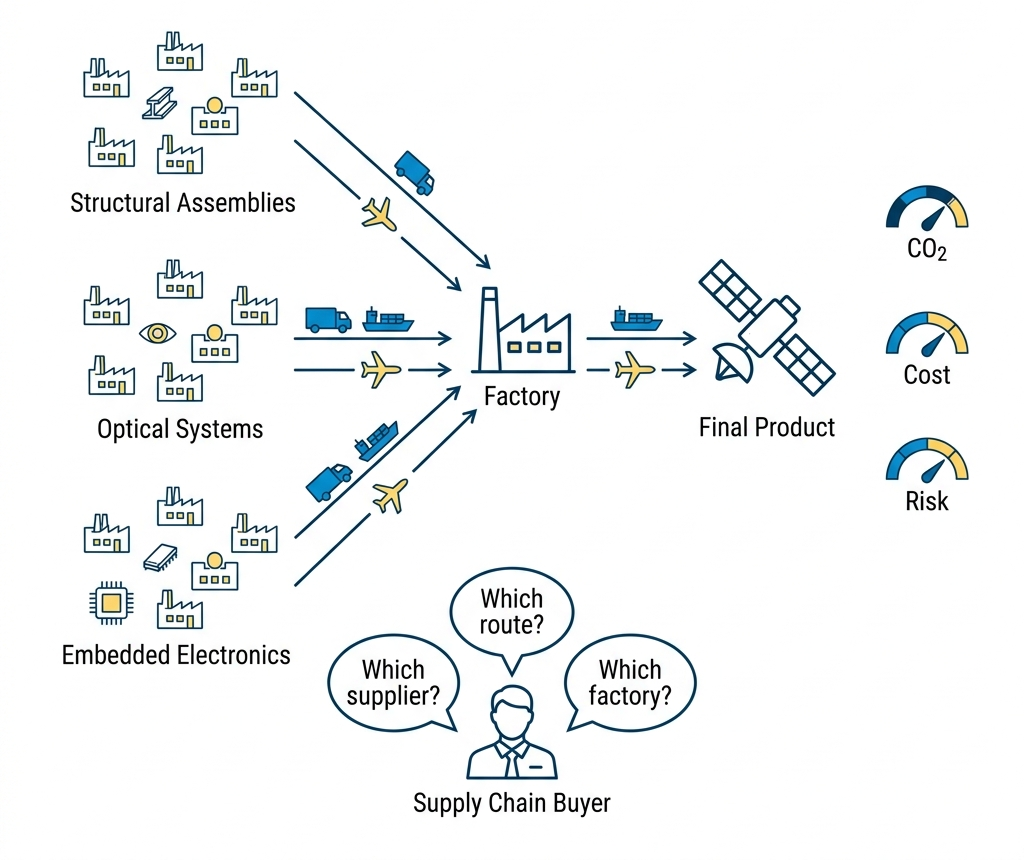
\includegraphics[width=0.82\linewidth]{Images/1.Introduction/disco_map.png}
    \caption{The DISCO serious game network}
    \label{fig:disco_map}
\end{figure}

Its scoring engine applies Min-Max normalisation over the values of the current game
session, illustrated here on the carbon dimension:

\begin{equation}
    \text{ScoreCO}_2 = 1 + 9 \times \frac{\text{realCO}_2 - \text{co}_{2,\min}}
                                         {\text{co}_{2,\max} - \text{co}_{2,\min}},
    \label{eq:score_co2}
\end{equation}

with analogous formulae for cost and risk, on a scale from 1 for the best achievable
performance to 10 for the worst.

\begin{table}[htbp]
\centering
\caption{DISCO technology stack}
\label{tab:disco_stack}
\begin{tabularx}{\linewidth}{lX}
\toprule
\textbf{Component} & \textbf{Technology / Value} \\
\midrule
Backend API    & Spring Boot + Java~21 \\
Database       & PostgreSQL (Azure) \\
Frontend       & Angular \\
Authentication & Player key / Azure AD SSO OAuth2 \\
Scores computed & CO\textsubscript{2}, Cost, Risk per supplier and itinerary, on $[1,10]$ \\
\bottomrule
\end{tabularx}
\end{table}

This work sits within a body of prior DIN research. \textcite{baxas2025architecture}
defines the DISCO software architecture including the \gls{tts} and \gls{ttr}
formalisation. \textcite{baulain2024internet} developed the Physical
Internet routing module, providing transit times through the HERE Maps API with Vincenty
distances and mandatory \gls{hgv} pause compliance, together with the Itinerary
Performance Index (\gls{ipg}) normalised on $[0,1]$.
\textcite{kabouche2025scoring} developed the supplier risk scorer combining delay
history, geographic vulnerability and financial fragility.
\textcite{cordova2024green} developed the per-route CO\textsubscript{2}
quantification module using the GLEC and VECTO methodology.
\textcite{mondelice2025tms} developed the Transport Management System interface
providing real-time transit-time extraction.

These works form the organisational and thematic context of the present research. The
system delivered here, named SupplyScore and described in Section~\ref{sec:methods_impl},
is a standalone Python application that runs alongside these modules rather than inside
them. Their coupling is a stated perspective of the programme, not a delivered capability,
and this thesis makes no claim to the contrary.

%% ─────────────────────────────────────────────────────────────────────────
\subsection{Problem Statement}
\label{sec:intro_problem}
%% ─────────────────────────────────────────────────────────────────────────

This thesis addresses the layer that comes \emph{before} any planning or scheduling
decision, and which the classical literature has not fully investigated: the urgency
signal itself is systematically biased at the source, and must be measured and corrected
before it can safely inform any downstream
decision~\autocite{zhu2018mere,rusou2020psychology}.

The consequences are worse where capacity is shared. In an interconnected network, a biased
urgency signal does not stay local: it propagates, and misallocation grows as it travels.
Over-triage, declaring more urgency than the situation warrants, takes capacity from
whoever needed it more. Under-triage does the opposite and is more dangerous, because a risk
nobody has declared is a risk nobody is
watching~\autocite{li2020exploring,ivanov2020digital}.

Digital twin architectures and real-time decision support systems have demonstrated strong
capabilities in operational monitoring, disruption detection, resource reallocation and
order synchronisation~\autocite{ding2023realtime,leung2022digital,hrusovsky2021realtime,karam2022realtime,zhu2025industry5}.
They do so primarily by computing the physical operational state of the system. To the
best of the review presented in Section~\ref{sec:Literature}, existing systems do not
explicitly model the gap between a declared urgency and a computed operational urgency.

Figure~\ref{fig:urgency_gap} shows what that gap looks like over the life of a task. Two
curves are plotted against time. The step line is declared urgency, which moves only when
the operator submits a review, and the smooth curve is real urgency, which moves as the
operational state does. Reading left to right, the figure passes through four phases: the
two signals agree, then a first adequacy defect opens, then a second defect of the opposite
sign, then agreement returns. Shading tells the two defects apart. Where the step line sits
above the curve the operator is claiming more urgency than the state justifies, and the
enclosed area is false urgency. Where the curve sits above the step line the state is worse
than anyone has declared, and the enclosed area is hidden risk. Leader lines pointing at a
curve label that signal; leader lines pointing into a shaded area label the gap between
them.

\begin{figure}[htbp]
    \centering
    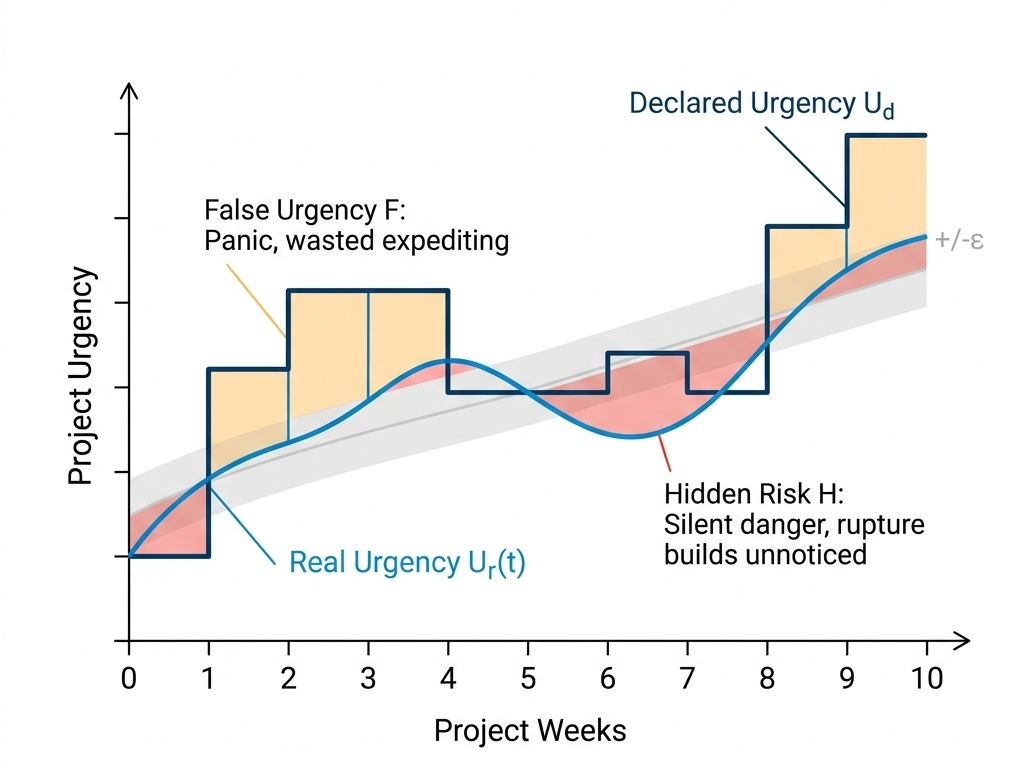
\includegraphics[width=0.82\linewidth]{Images/2.Problem/urgency_gap.png}
    \caption{Declared and real urgency, and the two mismatch pathologies}
    \label{fig:urgency_gap}
\end{figure}

Formally, let $U_d \in [0,1]$ denote the declared urgency and $U_r(t) \in [0,1]$ the real
urgency computed from operational data in the digital twin. The mismatch between the two
signals is

\begin{equation}
    \Delta U(t) = U_d - U_r(t) \in [-1,\, 1].
    \label{eq:delta_u}
\end{equation}

A tolerance band $\varepsilon \in [0,1]$ is introduced so that small deviations are not
treated as operationally meaningful. Over-declaration then corresponds to
$\Delta U(t) > \varepsilon$, under-declaration to $\Delta U(t) < -\varepsilon$, and
approximate agreement to $|\Delta U(t)| \le \varepsilon$. Table~\ref{tab:pathologies}
gives the operational reading of each condition.

\begin{table}[htbp]
\centering
\caption{Urgency pathologies and their consequences}
\label{tab:pathologies}
\small
\begin{tabularx}{\linewidth}{l >{\raggedright\arraybackslash}X >{\raggedright\arraybackslash}X}
\toprule
\textbf{Condition} & \textbf{Interpretation} & \textbf{Potential consequence} \\
\midrule
$\Delta U(t) > \varepsilon$ & Over-declaration of urgency, or false urgency & Excess
expediting, avoidable cost, possible delay for other flows \\[4pt]
$\Delta U(t) < -\varepsilon$ & Under-declaration of urgency, or hidden risk & Hidden
lateness or stockout risk, delayed intervention, downstream disruption \\[4pt]
$|\Delta U(t)| \le \varepsilon$ & Acceptable alignment & No material urgency mismatch \\
\bottomrule
\end{tabularx}
\end{table}

The two conditions need not cost the same. Weighting them asymmetrically, with
$\lambda_{\text{under}} \ge \lambda_{\text{over}}$, prices under-prioritisation above
over-prioritisation. Two bodies of work support doing so: operations research showing that
decision errors carry unequal downstream
consequences~\autocite{kim2020admission,diwa2020task}, and scheduling work that models
differentiated tardiness penalties instead of a uniform delay
cost~\autocite{baker1982dynamic,chakrabortty2022}. How much asymmetry is right is a
calibration question, answerable only in a specific setting.

%% ─────────────────────────────────────────────────────────────────────────
\subsection{Aim, Objectives and Research Questions}
\label{sec:intro_aim}
%% ─────────────────────────────────────────────────────────────────────────

The aim of this research is to establish whether the divergence between declared and
computed urgency is measurable to a standard that would justify acting on it.

That wording is deliberate on two counts. It commits to a falsifiable target rather than to
building a system: a score that cannot beat a trivial baseline against recorded outcomes has
not met the standard, however well engineered the system producing it. And it makes
measurability the question rather than assuming it, because the two signals being compared
are not independent by construction, and an architecture that lets the same person supply
both sides is measuring its own input.

Three objectives follow from that aim:

\begin{enumerate}[label=\textbf{O\arabic*.}]
    \item Define a multi-block, DAG-propagated real urgency $U_r(t)$ and a cognitive
          adequacy score $A(t) \in [0, 100]$ measuring the gap between the planner's
          declared urgency $U_d$ and the digital twin's operational state.
    \item Develop and implement a network propagation and criticality-driven
          prioritisation layer, combining PROMETHEE~II outranking with systematic shock
          simulation, to identify structurally critical nodes.
    \item Validate the resulting signal empirically, against recorded outcomes, and
          measure what happens to human declaration behaviour when the system's own
          forecast is placed in front of the declarant.
\end{enumerate}

Four research questions structure the scientific approach:

\begin{enumerate}[label=\textbf{RQ\arabic*}., leftmargin=*]
  \item \emph{Multi-block real urgency.} How can a physically and operationally grounded
  real urgency $U_r(t)$ be computed dynamically in a multi-tenant digital twin from
  heterogeneous KPI blocks, covering time, capacity, performance, risk, cost and
  environmental dimensions, and propagated coherently across a multi-tier supply chain
  graph?

  \item \emph{Cognitive adequacy formulation.} How should an adequacy score $A(t)$ be
  formulated to measure the alignment between declared urgency $U_d$ and computed real
  urgency $U_r(t)$ while asymmetrically penalising under-triage against over-triage, and
  does that score demonstrate predictive validity against recorded operational outcomes?

  \item \emph{Network prioritisation and criticality.} How can pairwise elicitation
  methods, namely AHP and the Fuzzy Best-Worst Method, be combined with outranking
  aggregation through PROMETHEE~II and systematic shock simulation to identify which nodes
  of a supply network are structurally critical?

  \item \emph{Operational validation and the effect of showing the forecast.} How can
  this framework be operationalised and empirically validated within a persistent digital
  twin exercised as a weekly-cadence serious game, and what happens to declared urgency
  once the declarant is shown the system's own prediction?
\end{enumerate}

The second half of RQ4 is not an afterthought. The campaign produced a result about the
declarant rather than only about the model, and reporting the model's scores without it
would be misleading (Section~\ref{sec:res_armB}).

%% ─────────────────────────────────────────────────────────────────────────
\subsection{Research Hypotheses}
\label{sec:hypotheses}
%% ─────────────────────────────────────────────────────────────────────────

These six hypotheses were pre-registered. They were written, with their numeric thresholds,
and frozen before the campaign of Section~\ref{sec:methods_campaign} produced any data, which
is why they appear here rather than next to the results they decide. They are reproduced
unchanged. Where the campaign later showed a threshold to be badly chosen, or a hypothesis to
be untestable on the scenario as scripted, that is reported as a finding in
Section~\ref{sec:hypothesis_status} and not repaired by rewriting the hypothesis.

Each states an observable outcome with a threshold the delivered system either meets or does
not, and each serves one of the research questions above.

\begin{description}
    \item[H1 (Cognitive latency):] Declared urgency follows computed real urgency with a
    delay of at least one weekly cycle on the majority of nodes. Test: the lagged
    correlation between $U_d$ and $U_r$ peaks at a lag of one week or more for at least
    five of the eight campaign nodes.
    \item[H2 (Early detection of hidden risk):] The hidden-risk signal
    $H = \max(U_r - U_d, 0)$ exceeds $0.3$ at the crisis-origin node several weeks before
    the rupture becomes publicly visible.
    \item[H3 (Structural criticality):] The systematic shock simulation ranks the true
    crisis origin first, by impact on the final customer, on at least 80\% of the
    informative, non-saturated weekly rounds.
    \item[H4 (Predictive validity):] At threshold $H \ge 0.5$ with a four-week horizon,
    the hidden-risk signal predicts recorded negative outcomes, meaning a missed
    milestone, a critical event or a node abandonment, with precision and recall both
    above $0.5$.
    \item[H5 (Urgency contagion):] On weeks when crisis news becomes public, operators of
    nodes that are not physically affected still raise their declared urgency,
    reproducing the mere-urgency effect~\autocite{zhu2018mere} at network scale.
    \item[H6 (Perception hysteresis):] Once the physical situation improves, declared
    urgency decays at less than half the rate of real urgency.
\end{description}

Table~\ref{tab:rq_hypothesis_map} maps each hypothesis to the question it serves and states
what its failure would mean, so that a negative result carries a consequence rather than
just a verdict.

\begin{table}[htbp]
\centering
\caption{Each hypothesis, its research question, and the cost of failure}
\label{tab:rq_hypothesis_map}
\small
\begin{tabularx}{\linewidth}{l >{\centering\arraybackslash}p{1.4cm} X}
\toprule
\textbf{Hypothesis} & \textbf{Serves} & \textbf{If it fails} \\
\midrule
H1 cognitive latency & RQ2 & Declared urgency tracks the physical signal without delay, so
there is no lag to correct and the adequacy layer has nothing to add. \\
H2 early detection & RQ2 & The hidden-risk signal arrives no earlier than the rupture it is
meant to anticipate, which makes it a description rather than a warning. \\
H3 structural criticality & RQ3 & The network ranking cannot be trusted to identify the
bottleneck, so criticality-driven prioritisation is unsafe to act on. \\
H4 predictive validity & RQ2 & The signal does not predict recorded outcomes, and the score
is a diagnostic curiosity rather than a decision aid. This is the hypothesis the aim of
Section~\ref{sec:intro_aim} stands or falls on. \\
H5 urgency contagion & RQ1, RQ4 & Operators do not import urgency from context, so
declaration bias is individual rather than systemic and does not propagate. \\
H6 perception hysteresis & RQ2 & Over-declaration corrects itself once the situation eases,
so the asymmetric penalty is mis-specified and $\lambda_{\text{under}}$ needs
recalibrating. \\
\bottomrule
\end{tabularx}
\end{table}

One omission from this register is worth flagging in advance, because
Section~\ref{sec:res_target_trap} measures its cost. The thresholds were pre-registered but
the definition of an adverse outcome was not, and that definition turns out to move the
measured result by more than the thresholds do.

Distinct from these testable hypotheses, the framework rests on stated modelling
assumptions, each verifiable in the delivered code: the network is a directed acyclic
graph, so there are no feedback loops and a linear topological sort is valid; reviews
follow a strict ISO weekly cycle; declared urgency is damped as it descends toward
suppliers while real risk is amplified as it ascends toward the customer, each scaled by a
per-arc coefficient; the six KPI blocks are treated as independent so that a probabilistic
aggregation is admissible; task statuses drive explicit override rules; and the cognitive
loss is deliberately asymmetric, with under-declaration priced at roughly twice the cost
of panic. These are design commitments, not empirical claims, and the limitations they
induce are catalogued in Section~\ref{sec:limitations}.

%% ─────────────────────────────────────────────────────────────────────────
\subsection{Scope and Delimitations}
\label{sec:intro_scope}
%% ─────────────────────────────────────────────────────────────────────────

Four boundaries are set explicitly, because each of them shapes what the results in
Section~\ref{sec:Results} can and cannot support.

\paragraph{The declarants are language-model agents, not human consultants.} The campaign
reported here was run with eight isolated language-model agents, one per role, each
confined to its own role card and turn briefings. This is an experimental design choice
with real consequences for external validity, discussed in
Sections~\ref{sec:methods_arms} and~\ref{sec:res_discussion}. The human campaign for which
the protocol was originally frozen has not been run.

\paragraph{The validation is a single scenario.} All results come from one pre-registered
scenario, a semiconductor shortage propagating through an eight-node satellite supply
chain over nineteen weekly turns. Statements about how the framework behaves are
statements about its behaviour on that scenario.

\paragraph{SupplyScore is standalone.} It does not integrate with DISCO, with an ERP, or with
the routing and carbon modules of Section~\ref{sec:intro_disco}. Every KPI reaching the
model arrives either through a manual weekly review or through a scripted campaign event.

\paragraph{The satellite observation work is an opening, not a second contribution.}
Section~\ref{sec:res_volume} reports a separate system that estimates warehouse capacity
from public satellite imagery. It is included because it addresses the freshness
limitation that the rest of this thesis documents about itself, and it is reported at the
depth that claim requires, without any assertion that the two systems have been connected.

%% ─────────────────────────────────────────────────────────────────────────
\subsection{Thesis Structure}
\label{sec:intro_structure}
%% ─────────────────────────────────────────────────────────────────────────

Four sections follow. Section~\ref{sec:Literature} reviews the streams that bear on the
problem and states the gap each one leaves. Section~\ref{sec:Methods} keeps three things
apart that are easily confused: the mathematical model, the choices made in building it into
software, and the experiment designed to test it. It closes with the method's own limits,
its reproducibility provisions and its ethics. Section~\ref{sec:Results} reports what was
measured, then diagnoses it. Section~\ref{sec:Conclusion} states what the work contributes,
what each hypothesis did, where the work stops, and what it opens.


\clearpage
\section{Literature Review}
\label{sec:Literature}
%% ═══════════════════════════════════════════════════════════════════════════
\subsection{Introduction and Key Definitions}
\label{sec:lit_intro}
%% ═══════════════════════════════════════════════════════════════════════════

This review answers a single question: which existing methods can be assembled to measure,
correct and propagate a biased urgency signal, and which part of that assembly is missing from
the literature? The relevant work is broad but fragmented across operations research,
behavioural science and digital twin engineering, and read individually each stream solves one
piece. Read together they leave a specific slot empty: no retrieved work combines, within a
single supply chain decision architecture, a multi-block operational urgency function, a
structured client-side urgency input, an adequacy layer comparing stated and operational
urgency, network propagation across a multi-tier DAG, and empirical validation of the adequacy
signal against recorded
outcomes~\autocite{sawik2013integrated,sawik2014joint,sawik2016integrated,cohen2021assigning,hosseini2020bayesian}.
The review is organised by the role each stream plays in that argument rather than by
chronology, 

Six terms carry specific meanings throughout. \textbf{Urgency} is how far a task needs prompt
action to avoid a material loss of operational performance; \emph{importance} is about
strategic value and \emph{priority} about current execution order, and a task can be important
and not urgent, or first in the queue for reasons connected to
neither~\autocite{cheng2025survey,zhu2018mere}. \textbf{Real-time scheduling} covers algorithms
assigning execution order under temporal and resource
constraints~\autocite{pinedo2012scheduling}, drawn on here only as historical grounding for
deadline-sensitive value functions, since no scheduling algorithm is delivered. A
\textbf{digital twin} is a synchronised digital representation of a physical system supporting
monitoring, simulation and decision-making from real-time and historical
data~\autocite{ivanov2020digital}. \textbf{\Gls{mcdm}} covers
methods combining potentially conflicting performance dimensions into a single
decision~\autocite{saaty1980analytic,brans1986promethee}. The \textbf{\Gls{pi}} is the model of open, mutualised logistics networks routing shipments through
shared infrastructure in standardised modular containers~\autocite{montreuil2011toward}. And a
\textbf{serious game} is a simulation environment designed to train decision-makers through
realistic scenarios with immediate feedback and
scoring~\autocite{sterman1989modeling,prensky2001digital}.

%% ═══════════════════════════════════════════════════════════════════════════
\subsection{Risk Propagation and Deadline-Sensitive Value}
\label{sec:lit_temporal}
%% ═══════════════════════════════════════════════════════════════════════════

Within real-time systems, deadline-sensitive scheduling theory models task value as a
function of completion or response time, an approach known as time-value or utility-accrual
scheduling~\autocite{cheng1996due,cheng2025survey}. Chen and
M\"uhlethaler~\autocite{cheng1996due} show that task utility is typically constant up to a
deadline and then non-increasing with delay, and a broader survey confirms that
deadline-sensitive literature models task value as a function of response time with
bounded, structured degradation after critical thresholds~\autocite{cheng2025survey}. This
establishes the precedent for treating urgency as time-varying, but it stops at a single
task in isolation.

A complementary line of evidence comes from network risk propagation. Ivanov and colleagues
formalise the ripple effect, whereby a local disruption at one supplier cascades through
downstream tiers and amplifies as it
travels~\autocite{ivanov2020digital,ivanov2019viable,li2020exploring}. Probabilistic risk
inference for supply chain systems~\autocite{Zhe20} further shows that aggregating
heterogeneous risk indicators into a single node-level score is itself an open modelling
question, distinct from how that score should then be propagated.

Table~\ref{tab:urgency_models} compares four candidate aggregation and growth models found
across these two lines, and Figure~\ref{fig:aggregation_families} plots what each one does.

\begin{figure}[htbp]
    \centering
    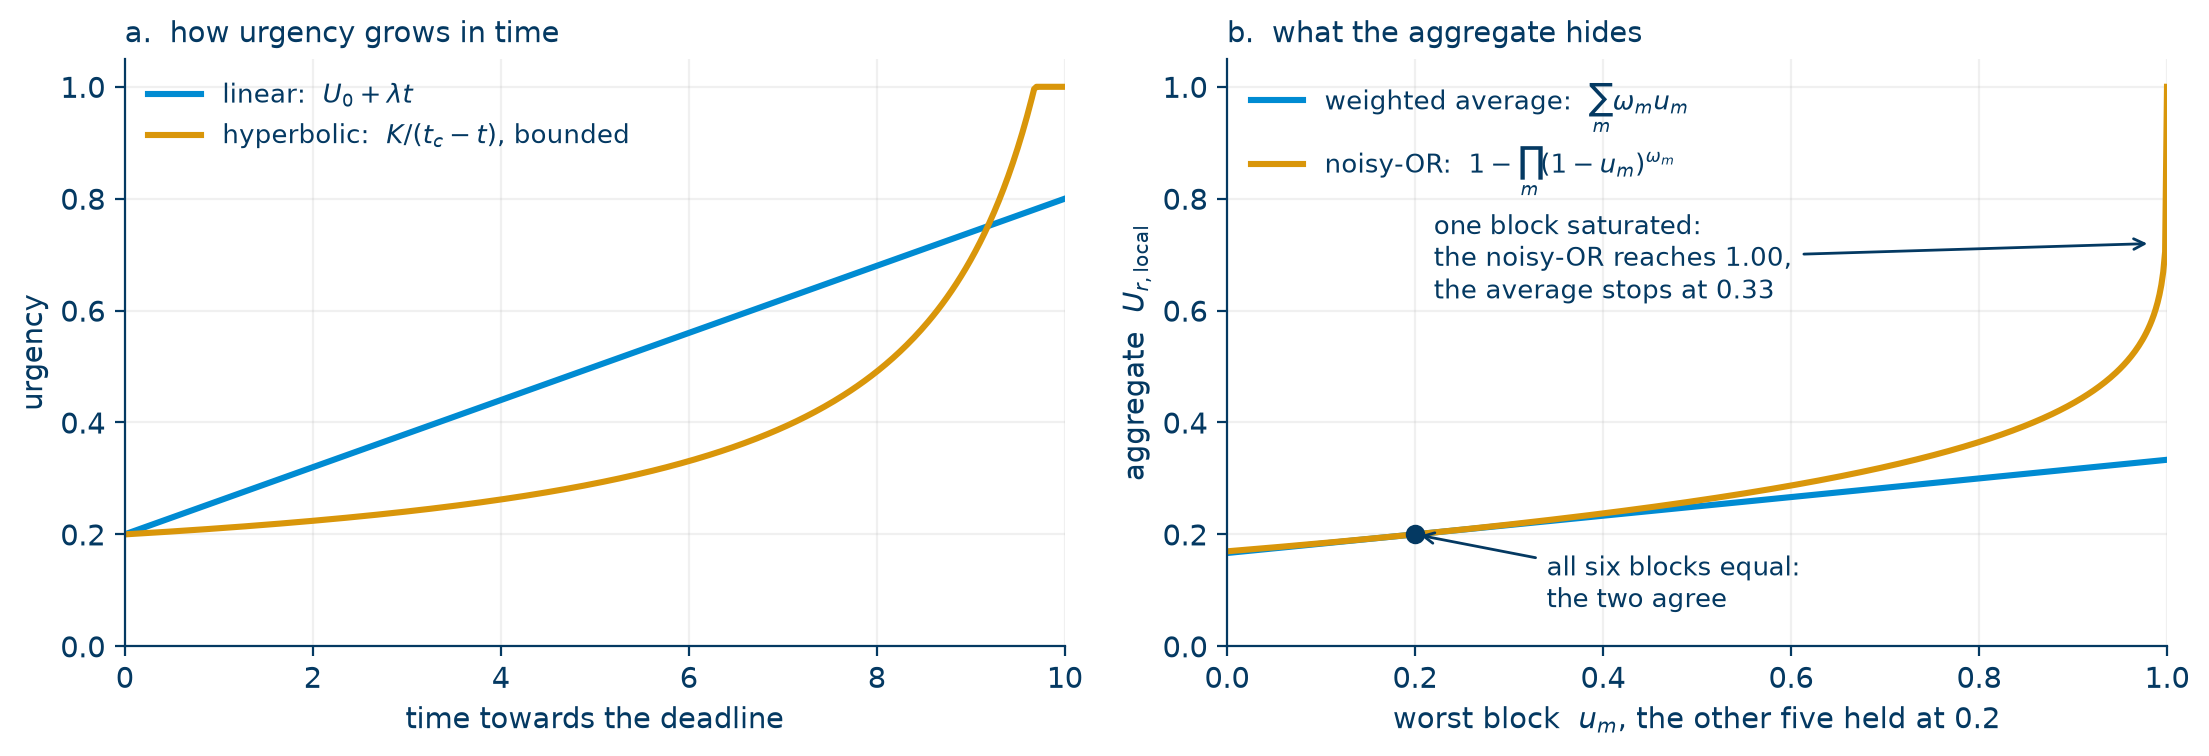
\includegraphics[width=\linewidth]{Images/aggregation_families.png}
    \caption[The four candidate models, plotted]{The four models of
    Table~\ref{tab:urgency_models}. Panel~b is the choice this thesis has to make: a weighted
    average is fully compensatory, so a catastrophic reading on one block is offset by
    acceptable readings elsewhere and the aggregate stops at $0.33$; a noisy-OR is not, and
    any factor approaching its maximum drives the aggregate towards its own maximum whatever
    the others read. Which behaviour is desirable depends on whether the aggregate describes
    average condition or exposure to the worst active cause, and the composite-indicator
    literature treats that as a modelling decision rather than a solved
    question~\autocite{greco2018,becker2017}.}
    \label{fig:aggregation_families}
\end{figure}

The hyperbolic family carries a further caveat. A structurally similar acceleration appears
in \gls{lppl} models of financial crash
precursors~\autocite{johansen2001finite,johansen2000crashes}, but empirical analyses find
LPPL-family models highly parameter-sensitive and unsuited to use as production risk
models~\autocite{feigenbaum2001statistical,bree2010prediction}.

\paragraph{Gaps in risk propagation and deadline-sensitive value.}
Neither stream specifies how to aggregate heterogeneous, block-structured operational risk
indicators at a single node before propagating them. Neither addresses declared urgency, or
the mismatch between what is stated and what is computable. And the aggregation literature
stops at the observation that the choice matters, without establishing whether equal values
on structurally different indicators carry equal risk meaning, which is the question any
multi-block aggregate has to answer before it can be interpreted.

%% ═══════════════════════════════════════════════════════════════════════════
\subsection{Cognitive Bias in Urgency Declaration}
\label{sec:lit_bias}
%% ═══════════════════════════════════════════════════════════════════════════

Human decision-makers systematically misrepresent urgency. Two lines of behavioural
operations research establish it from different angles, and both bear directly on any
system that takes operator-declared urgency as an input.

\textcite{zhu2018mere} report the Mere-Urgency Effect in five controlled experiments:
participants consistently over-prioritised imminent low-value tasks over distant
high-value tasks, and the bias persisted even when participants were informed of its
existence. \textcite{steel2006integrating} provides a complementary formal model
through the \gls{tmt}:

\begin{equation}
    V(t) = \frac{U \times E}{1 + \Gamma \times D(t)^k},
    \label{eq:tmt_val}
\end{equation}

where $U$ is objective utility, $E$ is the expectancy of success, $D(t)$ is the delay to
deadline, and $\Gamma$ and $k$ are individual discounting parameters. As the delay to
deadline shrinks towards zero, the motivational value $V(t)$ converges to the full product
of utility and expectancy, so immediacy becomes more salient as the deadline approaches.
Near-term tasks can therefore attract disproportionate attention even when their broader
objective value is lower~\autocite{steel2006integrating}.
Table~\ref{tab:tmt_vars} gives the operational role of each parameter.

These laboratory findings are supported by evidence from operational settings. \textcite{rusou2020psychology} show that operators under workload preferentially
complete small, easy tasks, the operational analogue of under-triage for large-scope supply
chain activities. \textcite{diwa2020task} confirm in a large field study
that completing easy tasks first significantly hurts overall performance. Hospital
admission control under occupancy uncertainty~\autocite{kim2020admission} produces over-
and under-triage patterns analogous to those seen in logistics operators facing uncertain
lead times. Human-centred decision support systems such as that of \textcite{rosenthal2020human} use visual feedback to show the mismatch between human
plans and system temporal constraints, helping users calibrate their schedules.

\paragraph{Gaps in cognitive bias research.}
Behavioural research diagnoses the problem and quantifies it in controlled settings, but
the magnitude of the bias in industrial supply chain contexts remains a matter of
calibration, and this literature does not prescribe a real-time operational correction.

%% ═══════════════════════════════════════════════════════════════════════════
\subsection{Indicators of Delivery Rupture Risk}
\label{sec:lit_indicators}
%% ═══════════════════════════════════════════════════════════════════════════

If urgency is to be aggregated from several indicators, the literature has to supply the
indicators. This section reviews the body of work that identifies which observable
quantities precede a delivery rupture, meaning a failure to deliver at the agreed time,
place, quantity and quality. It is the source from which
Section~\ref{sec:model_blocks} later selects.

Heckmann, Comes and Nickel establish rupture as the terminal event a supply risk measure
should anticipate, and criticise the field for measuring exposure without connecting it to
that event~\autocite{heckmann2015critical}. Indicator-based supplier monitoring proceeds by
identifying observable precursors rather than modelling the event
directly~\autocite{mokhtar2019supplier}.

Table~\ref{tab:precursors} gives the five families of precursor that recur across that work,
with the sources establishing each and the reason it is a precursor rather than a symptom.
Section~\ref{sec:model_blocks} selects from this table, and Section~\ref{sec:model_blocks} states what it kept.

\paragraph{Gap in the indicator literature.}
The families are named individually and no retrieved work supplies a criterion for deciding
which of them belong in one composite, nor a rule for combining them once chosen. That is the
question Section~\ref{sec:model_ur} answers with an explicit independence assumption rather
than with a weighting convention.

\subsection{Closest Antecedents: Network Risk Twins and MCDM Supplier Scoring}
\label{sec:lit_antecedents}
%% ═══════════════════════════════════════════════════════════════════════════

The works most structurally similar to this thesis combine multi-criteria supplier scoring
with disruption-aware network monitoring.
\textcite{sawik2013integrated} develops mixed-integer programming models for resilient
supplier order assignment integrating cost, service level and disruption risk, extended in
later work to joint and integrated
formulations~\autocite{sawik2014joint,sawik2016integrated}. \textcite{cohen2021assigning} and \textcite{afrasiabi2022extended}
extend this to \gls{mcdm} supplier prioritisation under disruption, combining criteria
weighting with allocation optimisation. \textcite{chakrabortty2020efficient} confirm that rule-based heuristics remain
competitive against exact methods in dynamic industrial environments. These works are cited
for the closeness of their subject matter, not because this thesis reuses their
optimisation machinery, which addresses allocation and sequencing rather than urgency
measurement.

\paragraph{Gaps in the closest antecedents.}
Two gaps distinguish this stream from the present work. First, none introduces a
network-propagated urgency signal computed independently at every node and combined across
tiers; risk is typically evaluated once, at the point of decision. Second, none compares a
client-stated urgency against a model-derived urgency: where the declared signal exists at
all, it is used directly, without validation against live operational proxies.

%% ═══════════════════════════════════════════════════════════════════════════
\subsection{Enabling Method: Bayesian and Probabilistic Risk Updating}
\label{sec:lit_bayes}
%% ═══════════════════════════════════════════════════════════════════════════

Bayesian methods are a well-supported approach for revising risk estimates from new
evidence in supply chain
research~\autocite{pearl1988probabilistic,koller2009probabilistic}. Rather than a full
Bayesian network with an explicit conditional-probability-table structure, this study draws
on the narrower and more tractable case of Beta-Bernoulli conjugate updating: a failure
probability $p$ is treated as a Beta-distributed belief with an equivalent prior sample
size $n_0$, revised from a small number of newly observed equivalent trials $(k, n)$ each
time a calibrated operational event is declared.

Three convergent findings support this choice. \textcite{hosseini2020bayesian} survey Bayesian methods applied to supply chain risk
and resilience, finding that probabilistic belief-revision methods are often preferred to
deterministic scoring when sparse new evidence must update an existing estimate. \textcite{huang2020bayesian} and \textcite{deng2020prediction}
develop Bayesian models for disruption and delay probability estimation.
\textcite{lockamy2011bayesian} and \textcite{qazi2017dynamic} support
Bayesian revision as a practical tool under sparse, event-driven evidence, consistent with
the small-sample setting of a weekly-cadence digital twin. Plain frequency counts, by
contrast, are unstable when only a handful of events are declared per node per
project~\autocite{zheng2020risk}.

\paragraph{Gaps in Bayesian risk updating.}
Bayesian belief revision quantifies disruption exposure but does not, by itself, compare it
against a client-declared urgency, and it says nothing about whether the resulting
probabilities are well calibrated once they reach a human reader.

%% ═══════════════════════════════════════════════════════════════════════════
\subsection{Enabling Method: Digital Twins and Real-Time Decision Support}
\label{sec:lit_dt}
%% ═══════════════════════════════════════════════════════════════════════════

The digital twin concept was formalised by \textcite{grieves2014digital} as a
virtualised representation of a physical process. \textcite{tao2018digital}
extended it to manufacturing, and \textcite{fuller2020digital} surveyed the
enabling technologies. In supply chain management, \textcite{ivanov2021digital} define the \gls{sc} \gls{dt} as integrating simulation,
optimisation and machine learning. \textcite{ivanov2020digital} address
digital supply chain twins for disruption risk and resilience management. \textcite{wang2020digital} demonstrate twin-driven planning in a manufacturing context
analogous to DISCO's satellite component network. In the Industry~5.0 setting, these
systems have evolved towards human-in-the-loop Cognitive Digital Twins, where semantic
models and reasoning methods capture human feedback and synchronise mental models with
simulated physical operations~\autocite{niloofar2023}.

Real-time freight planning work shows that operational urgency proxies, meaning slack,
lateness risk and shortage exposure, are already present within these
systems~\autocite{hrusovsky2021realtime,perez2022digital}. Model-predictive control for
vehicle routing~\autocite{karam2022realtime} and twin-based disruption
response~\autocite{ding2023realtime,leung2022digital,zhu2025industry5} confirm the state of
the art in live operational replanning.

\paragraph{Gaps in digital twin decision support.}
In the retrieved literature, no system combines a declared urgency input, a computed
operational urgency, and their propagated mismatch within one architecture. A second gap
matters for this thesis specifically: these systems are evaluated on the accuracy of their
physical state estimation, and their inputs are assumed to arrive. Where an input depends
on the same operator whose judgement the system exists to support, that circularity is not
usually treated as a measurement problem.

%% ═══════════════════════════════════════════════════════════════════════════
\subsection{Enabling Methods: Multi-Criteria Decision Methods}
\label{sec:lit_mcdm}
%% ═══════════════════════════════════════════════════════════════════════════

This research builds on two distinct domains within multi-criteria decision-making:
pairwise comparison methods for eliciting weights, and outranking aggregation for turning
those weights into a defensible ranking of nodes.

Table~\ref{tab:mcdm} compares the four methods on the three axes that decide which is usable
here: what an elicitation costs the operator, what the method returns, and whether a good
score on one criterion can hide a bad score on another.

The last column of that table is why both an elicitation method and an outranking method are
used rather than one. Weighted averages are fully compensatory: an excellent score on one
criterion masks a critical failure on another. Outranking builds pairwise preference flows
instead, which prevents that masking, and a cross-industry survey confirms its suitability for
supplier and node evaluation. Composite-index work nonetheless warns that nominal weights
often diverge from effective importance through correlation, normalisation and aggregation
dynamics, and that the choice of normalisation is itself non-neutral because it can produce
rank reversal~\autocite{greco2018,becker2017,triantaphyllou2000multi}.

\paragraph{Gaps in multi-criteria decision methods.}
These methods weight criteria and rank alternatives, and they are static elicitation and
aggregation tools. None is routinely compared against a computed operational counterpart. And
the composite-indicator critique is generally raised as a caveat at the end of a paper rather
than turned into something a running system can check on its own data.

\subsection{Forecast-Assisted Decision and Automation Bias}
\label{sec:lit_automation}
%% ═══════════════════════════════════════════════════════════════════════════

The streams above concern how to compute a signal. This one concerns what happens when the
signal is shown to the person whose judgement it was built to support, and it is included
because the campaign reported in Section~\ref{sec:res_armB} produced a result in exactly
that register.

\textcite{parasuraman1997humans} set out the canonical taxonomy of
misuse, disuse and abuse of automation, establishing that the failure modes of automated
aids are as much about human reliance as about machine accuracy. \textcite{skitka1999automation} demonstrate automation bias directly: participants
supported by an automated aid committed both omission errors, failing to react to a problem
the aid did not flag, and commission errors, following the aid against contradicting
evidence. \textcite{cummings2004automation} extends the finding to time-critical
decision support, the family to which a weekly supply chain review belongs. \textcite{goddard2012automation} provide a systematic review in clinical
decision support, and report that automation bias is frequent, that it is mediated by the
confidence with which advice is presented, and that it is only partially mitigated by
training.

The direction of the effect is not uniform. \textcite{dietvorst2015algorithm} document algorithm aversion, where people abandon
an algorithm after seeing it err even when it outperforms them, while
\textcite{logg2019algorithm} document algorithm appreciation, where
people weight algorithmic advice more heavily than human advice. \textcite{bansal2021whole} show that adding explanations to a model's output can
increase acceptance of its recommendations whether or not those recommendations are
correct, so that explanation improves persuasion more reliably than it improves joint
accuracy.

Two consequences follow for the present work. First, an advisory signal changes the
behaviour it measures, which means a system that both elicits declared urgency and displays
a forecast to the declarant is not observing an independent signal. Second, a confidently
presented but poorly calibrated probability is a specific hazard rather than a cosmetic
defect, since the confidence with which advice is presented is itself a mediator of
reliance~\autocite{goddard2012automation}.

\paragraph{Gaps in forecast-assisted decision research.}
This literature is dominated by single-decision laboratory tasks and clinical decision
support. It does not address a repeated, multi-turn setting in which the same operator is
shown a forecast about their own node, week after week, while their declaration feeds back
into the model's state. Nor does it address the case where the displayed forecast is
systematically miscalibrated in a known direction, which is the situation measured in
Section~\ref{sec:res_armA_scored}.

%% ═══════════════════════════════════════════════════════════════════════════
\subsection{Validation Methodology: Serious Games}
\label{sec:lit_games}
%% ═══════════════════════════════════════════════════════════════════════════

The Beer Game~\autocite{sterman1989modeling} is the foundational supply chain serious game.
Sterman shows that players systematically misperceive the feedback in their own supply
line, underestimating orders already placed but not yet received, and over-order with a lag
once a shortage appears, amplifying the resulting oscillation as it travels upstream, the
mechanism known as the bullwhip effect~\autocite{lee1997bullwhip}. This decision bias is
analogous to the false-urgency pathology, where an operator over-reacts to a signal after a
delay rather than adjusting smoothly. \textcite{prensky2001digital} establishes the
theoretical basis for digital game-based learning, and \textcite{deterding2011game} formalise gamification design principles.

\textcite{mohaddesi2020gamettes} introduce the Gamette methodology, a
bite-sized approach to capturing decision-making patterns for behavioural modelling,
directly applicable to a weekly-review protocol in which operators repeatedly submit
urgency assessments. \textcite{bellotti2013framework} provide an evaluation
framework for serious game learning outcomes. \textcite{lafkihi2025freight} use a freight transportation game to study carrier
behaviour on online spot-market platforms, a setting connected to the Physical Internet's
vision of mutualised capacity allocation.

\paragraph{Gaps in serious game validation.}
Serious games are established as instruments for observing decision bias, but they are
usually scored on learning outcomes or on aggregate system performance. They are rarely
used as a controlled comparison in which the same frozen scenario is replayed with and
without a treatment applied to the declarant, which is the design adopted in
Section~\ref{sec:methods_arms}.

%% ═══════════════════════════════════════════════════════════════════════════
\subsection{Probabilistic Forecast Verification}
\label{sec:lit_verification}
%% ═══════════════════════════════════════════════════════════════════════════

Because this thesis scores a probabilistic forecast against recorded outcomes, it inherits
the vocabulary of forecast verification. \textcite{brier1950verification} introduced
the mean squared error of probabilistic forecasts, and
\textcite{murphy1973vector} decomposed it into reliability, resolution and
uncertainty, establishing the distinction this thesis relies on: a forecast can order
outcomes correctly while announcing the wrong probabilities, and the two failures require
different remedies. \textcite{gneiting2007strictly} formalise strictly
proper scoring rules, under which a forecaster minimises expected loss only by reporting
their true belief.

The distinction has been rediscovered in machine learning. \textcite{niculescu2005predicting} show that several strong classifiers produce
distorted probabilities that require post-hoc correction, and \textcite{guo2017calibration} show that modern neural networks are systematically
over-confident, with accuracy improving while calibration degrades. Both report that the
correction is a separate, cheap, post-hoc layer rather than a change to the model.

\paragraph{Gaps in forecast verification practice.}
The verification literature assumes the outcome being predicted is unambiguously defined.
In an operational supply chain setting it is not: whether a node-week counts as an adverse
outcome depends on choices about which events qualify and over what horizon.
Section~\ref{sec:res_target_trap} shows that this choice, and nothing else, moves the
measured skill of the same forecasts by a factor of five.

%% ═══════════════════════════════════════════════════════════════════════════

\subsection{Analogical and Contextual Literature}
\label{sec:lit_analogy}
%% ═══════════════════════════════════════════════════════════════════════════

Three streams provide vocabulary and context rather than foundations, and are flagged as
non-foundational wherever they are used.

\paragraph{Medical triage as a conceptual analogy.}
Medical triage provides an analogy for prioritising under severe capacity constraints and
cognitive pressure. Protocols such as the \gls{mts}~\autocite{mackway2013emergency} categorise patients into five urgency levels
using flowcharts, whereas the Emergency Severity Index integrates predicted resource
consumption. Comparative clinical studies show substantial classification discrepancies between the two
systems, at a weighted $\kappa = 0.51$, so even trained professionals disagree on urgency
assessment~\autocite{kuligowski2025comparative}. The clinical literature also establishes an
asymmetry that logistics work rarely states explicitly: under-triage, meaning a patient
classified as less urgent than they are, is more dangerous than over-triage, because the
first costs a life and the second costs a
queue~\autocite{kim2020admission,mackway2013emergency}.

\paragraph{Physical Internet and synchromodality.}
The Physical Internet is a model of interconnected logistics networks in which routing,
storage and transport assets are mutualised across actors~\autocite{montreuil2011toward}. In
such networks urgency stops being a local concern and becomes a network-level quality of
service variable, because the capacity one actor claims is capacity another loses.

A related but separate concept is synchromodality. Where the Physical Internet describes who
shares the infrastructure, synchromodality describes when the mode is chosen: a shipment can
be moved between road, rail and waterway in real time as conditions change, instead of
being committed to one mode when it is booked. The two can operate together and neither
presupposes the other. Dynamic routing under synchromodality needs priority signals that
stay valid across rolling planning windows~\autocite{guo2020dynamic}, and disruptions travel
quickly through interconnected networks, producing cascading ripple
effects~\autocite{li2020exploring}.

\paragraph{Regulatory carbon accounting.}
Corporate sustainability reporting requirements have made transport emissions a reported
quantity rather than an optional one~\autocite{cordova2024green}. The \gls{glec} Framework
v3.2~\autocite{smartfreight2023glec} and \gls{vecto}~\autocite{commission2017vecto} define
emissions baselines for heavy goods vehicles, and emissions factors relate non-linearly to
vehicle speed and cargo load, so a carbon figure cannot be recovered from cost or distance
alone~\autocite{ademe2014impacts}.

\paragraph{Earth observation of built and logistics assets.}
The opening reported in Section~\ref{sec:res_volume} rests on a separate literature.
Overhead object detection has a standard benchmark in DOTA~\autocite{xia2018dota}, whose
oriented bounding boxes and vehicle classes make it the reference for overhead vehicle
detection, while
building footprint extraction is benchmarked by
Inria~\autocite{maggiori2017inria} and SpaceNet~\autocite{vanetten2018spacenet}.
Promptable segmentation foundation models~\autocite{kirillov2023segment} have made it
possible to sample candidate sites from imagery alone rather than from a cadastral
database. Separately, a body of economics work establishes that satellite observation can
serve as an independent proxy for activity that official statistics record slowly or not at
all, from night-time lights as a growth proxy~\autocite{henderson2012measuring} to
daytime imagery as a poverty predictor~\autocite{jean2016combining}.

\paragraph{Gap in Earth observation for supply chain state.}
That economics literature measures aggregate activity at regional scale. It does not
produce the per-facility quantities a supply chain twin needs, meaning storable volume and
transfer capacity at a named site, and the detection literature stops at footprints and
vehicles without converting them into an operational capacity figure.

%% ═══════════════════════════════════════════════════════════════════════════
\subsection{Source Review Grid}
\label{sec:lit_grid}
%% ═══════════════════════════════════════════════════════════════════════════

Each source analysed above is synthesised in an evaluation grid recording its main argument,
methodological approach, conclusions, thematic relevance and a critical appraisal of its
limitations. The grid is given in Appendix~\ref{app:source_grid}, and it makes explicit which
claims in this thesis rest on foundational work and which rest on analogy.

%% ═══════════════════════════════════════════════════════════════════════════
\subsection{Identified Gaps}
\label{sec:lit_gaps}
%% ═══════════════════════════════════════════════════════════════════════════

Each stream above closes on the limit of what it settles, and collected those limits describe
one absence rather than several. Figure~\ref{fig:lit_map} places each stream against
the two things this thesis needs from it, and the empty column is the gap.

\begin{figure}[htbp]
\centering
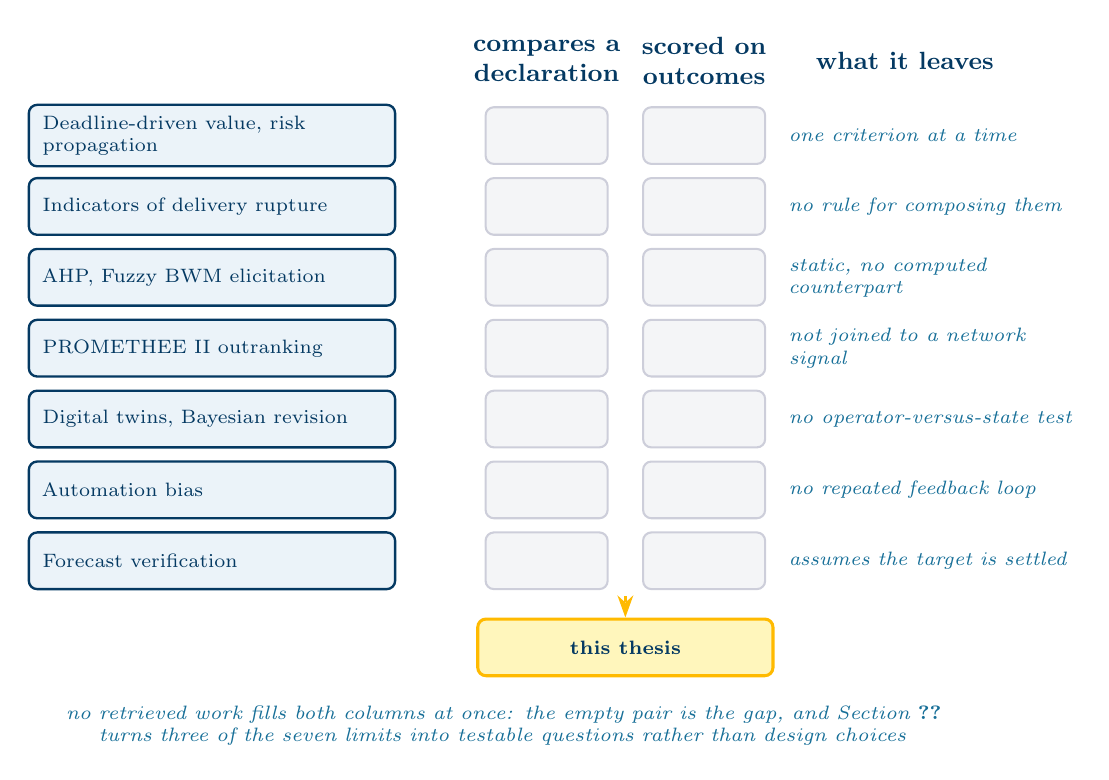
\begin{tikzpicture}[x=1cm, y=1cm, font=\scriptsize,
    st/.style  = {bloc, text width=4.3cm, minimum height=0.72cm, align=left,
                  inner xsep=5pt},
    yes/.style = {blocFort, minimum width=1.55cm, minimum height=0.72cm},
    no/.style  = {blocPale, minimum width=1.55cm, minimum height=0.72cm}]

\node[titreBande, align=center, text width=1.9cm] at (7.55, 4.35)
     {compares a\\declaration};
\node[titreBande, align=center, text width=1.9cm] at (9.55, 4.35)
     {scored on\\outcomes};
\node[titreBande] at (12.1, 4.35) {what it leaves};

\foreach \y/\lab/\gap in {
   3.4/{Deadline-driven value, risk propagation}/{one criterion at a time},
   2.5/{Indicators of delivery rupture}/{no rule for composing them},
   1.6/{AHP, Fuzzy BWM elicitation}/{static, no computed counterpart},
   0.7/{PROMETHEE~II outranking}/{not joined to a network signal},
   -0.2/{Digital twins, Bayesian revision}/{no operator-versus-state test},
   -1.1/{Automation bias}/{no repeated feedback loop},
   -2.0/{Forecast verification}/{assumes the target is settled}}
{
  \node[st] (s\y) at (3.3, \y) {\lab};
  \node[no]  at (7.55, \y) {};
  \node[no]  at (9.55, \y) {};
  \node[etiquette, anchor=west, fill=none, text width=3.6cm, align=left]
       at (10.55, \y) {\gap};
}

\node[blocFort, minimum width=3.75cm, minimum height=0.72cm, draw=altenOchreDark,
      fill=altenOchrePale!55!white, line width=1.1pt] (gapcell) at (8.55, -3.1)
     {\textbf{this thesis}};
\draw[flecheCoupee] (8.55, -2.45) -- (gapcell.north);

\node[etiquette, anchor=north, text width=11.5cm] at (7.0, -3.75)
     {no retrieved work fills both columns at once: the empty pair is the gap, and
      Section~\ref{sec:Methods} turns three of the seven limits into testable questions
      rather than design choices};

\end{tikzpicture}
\caption[The literature map and the gap]{Each stream against the two properties this work
requires: that it compare a human declaration with a computed state, and that it be scored
against recorded outcomes. Every retrieved stream leaves at least one of the two empty, and
none fills both.}
\label{fig:lit_map}
\end{figure}

No retrieved work combines those streams with a structured declared-urgency input and an
empirically tested adequacy layer. That missing combination is the gap, and closing it is the
contribution this thesis claims: a measurement of the divergence between declared and computed
urgency, propagated across a supplier network, and scored against recorded outcomes rather than
asserted. Three of the gaps become testable questions rather than design choices, and they are
the ones carried into Section~\ref{sec:Methods}: whether the divergence can be measured at all
once both signals come from independent sources, whether the resulting signal predicts
anything, and what happens to the declared side when the computed side is shown to the person
declaring.


\clearpage
\section{Methods}
\label{sec:Methods}
%% ═══════════════════════════════════════════════════════════════════════════
\subsection{Methodological Framework}
\label{sec:methods_framework}
%% ═══════════════════════════════════════════════════════════════════════════

This research is structured as an agile test-and-learn programme rather than a linear
sequence, operating through repeated iterations of literature analysis, mathematical
specification, software implementation and scenario-based simulation
(Figure~\ref{fig:test_learn_loop}). That structure is mapped onto the IMRaD form of this
thesis as follows: the specification and implementation iterations are reported in this
section as the method, and the simulation and campaign iterations are reported in
Section~\ref{sec:Results} as the results.

The programme is organised into four operational areas:

\begin{itemize}
    \item \textbf{Literature review and gap analysis}, establishing the psychological and
          mathematical foundations of multi-block urgency aggregation and cognitive bias
          (Section~\ref{sec:Literature}).
    \item \textbf{Mathematical framework specification}, deriving the multi-block real
          urgency function, its DAG propagation and the asymmetric adequacy score from
          first principles, so that the result is dimensionally and probabilistically
          consistent (Section~\ref{sec:math_framework}).
    \item \textbf{Pairwise comparison elicitation}, formulating crisp AHP and Fuzzy
          Best-Worst Method weight vectors to build a structured representation of
          declared urgency (Section~\ref{sec:ahp_tool}).
    \item \textbf{Implementation, simulation and validation}, building a modular, tested
          Python library exercised through a multi-page Dash web application, running
          controlled shock and scenario simulations on a persistent digital twin, and
          confronting the resulting signal with recorded outcomes through a dedicated
          calibration service and a serious game campaign
          (Sections~\ref{sec:methods_impl} and~\ref{sec:methods_campaign}).
\end{itemize}

The remainder of this section keeps three things apart, because mixing them is what makes a
framework of this kind hard to read. Section~\ref{sec:math_framework} states the
mathematical model on its own terms, saying nothing about tooling.
Section~\ref{sec:methods_impl} gives the application choices, meaning how each object in
that model is elicited, computed and exposed. Section~\ref{sec:methods_campaign} gives the
use case built to test it. The method's own limitations, its reproducibility provisions and
its ethical considerations close the section.

\subsubsection{The Proposed Structure}
\label{sec:methods_axis}

Section~\ref{sec:lit_gaps} identified one absence rather than several. The response designed
here is a two-layer loop, and stating it before the mathematics makes the equations that
follow easier to place.

The first layer is a cognitive adequacy check. It captures the operator's declared urgency
$U_d$ through consistency-gated pairwise comparisons, computes a real urgency $U_r(t)$ from
live operational state, and scores their mismatch through an asymmetric penalty. The second
layer propagates and prioritises. Local urgency travels across the supply network, declared
urgency descending toward suppliers and real risk ascending toward the final customer, and
the resulting network state feeds an outranking and a shock-simulation criticality index that
together indicate which nodes warrant attention. Figure~\ref{fig:three_layer} shows how the
two layers sit relative to each other and where the declared and computed signals meet.

Two choices inside that design are worth naming immediately, since
Section~\ref{sec:lit_temporal} left both open. The aggregation over blocks is a noisy-OR
rather than a weighted average, because a complete capacity failure should not be offset by
acceptable cost and carbon readings, and non-compensatory behaviour is the property that
guarantees it. The penalty over the mismatch is asymmetric, pricing under-declaration above
over-declaration, on the clinical analogy of Section~\ref{sec:lit_analogy}, where
under-triage costs more than a queue. Both are design commitments open to challenge, and
Section~\ref{sec:limitations} records what each one costs.

\begin{figure}[htbp]
    \centering
    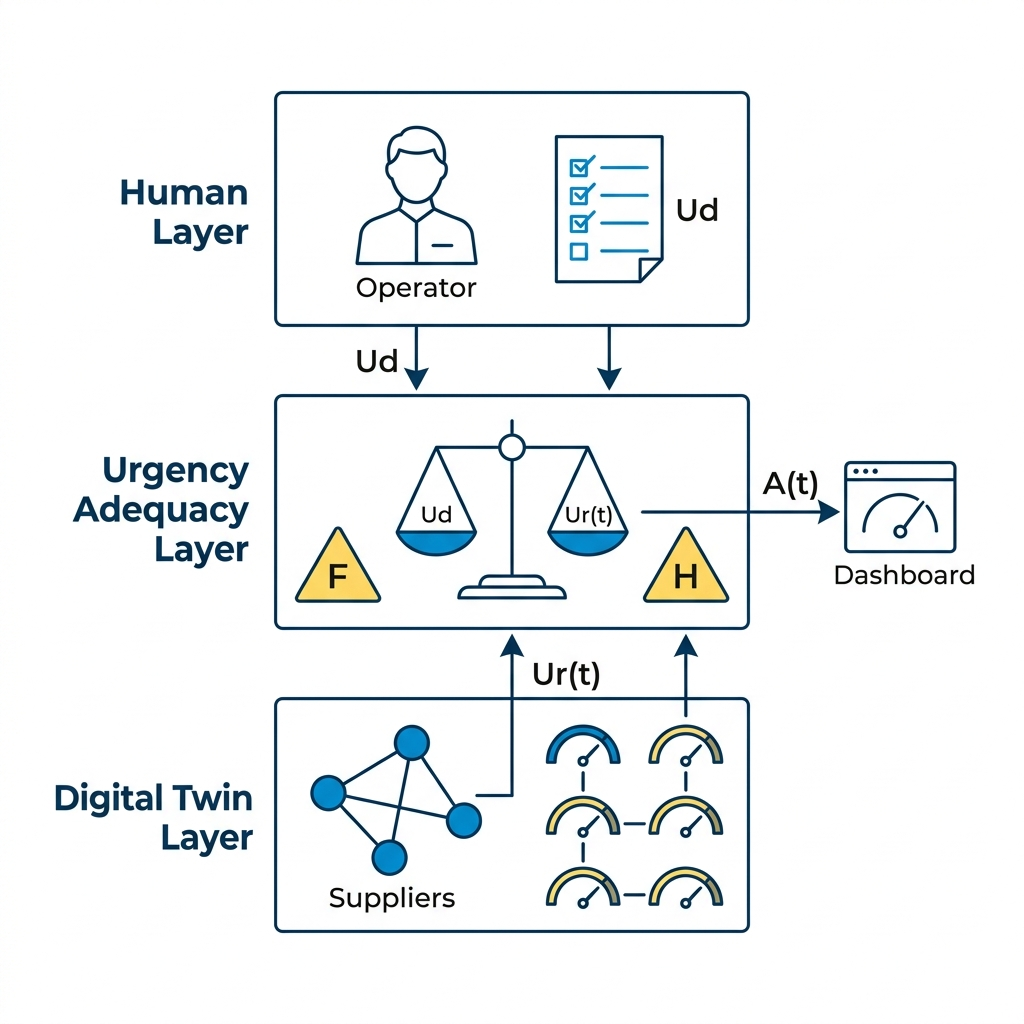
\includegraphics[width=0.82\linewidth]{Images/2.Problem/three_layer_architecture.png}
    \caption{The layered adequacy architecture}
    \label{fig:three_layer}
\end{figure}

\begin{figure}[htbp]
    \centering
    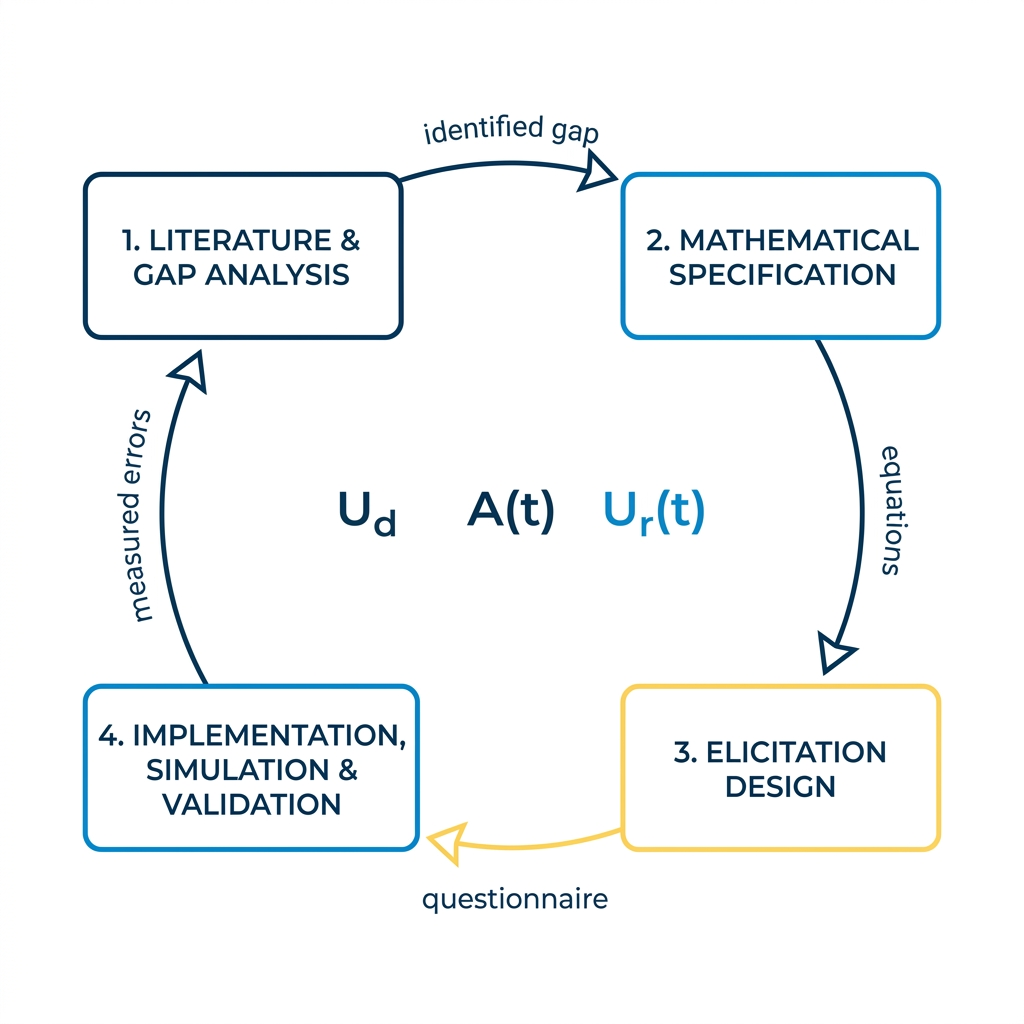
\includegraphics[width=0.82\linewidth]{Images/4.Operations/test_learn_loop.png}
    \caption{The test-and-learn iteration loop}
    \label{fig:test_learn_loop}
\end{figure}

%% ═══════════════════════════════════════════════════════════════════════════
\subsection{Mathematical Model}
\label{sec:math_framework}
%% ═══════════════════════════════════════════════════════════════════════════

This section states what real urgency and declared urgency are, how each propagates across
the network, and how their mismatch is scored. It deliberately leaves out tooling,
elicitation mechanics and operational cadence, which are application decisions addressed in
Section~\ref{sec:methods_impl}.

\subsubsection{Local Real Urgency}
\label{sec:model_ur}

Real urgency is not read from a single deadline-proximity signal. It is aggregated at each
node from six independent KPI blocks, namely time, capacity, performance, risk, cost and
carbon, each producing a partial urgency $u_m \in [0,1]$, or no value at all when the
underlying KPI data is unavailable. The aggregation is a weighted probabilistic OR, so that
a single saturated block is sufficient to drive local urgency toward its maximum regardless
of how well the others score:

\begin{equation}
    U_{r,\text{local}} = 1 - \prod_{m} (1 - u_m)^{\omega_m},
    \label{eq:ur_local}
\end{equation}

where $\omega_m \ge 0$ is the aggregation weight of block $m$ and the product runs over
blocks with available data. Table~\ref{tab:ur_blocks} gives each block's schematic formula
and what it measures. The notation $[x]_+ = \max(x, 0)$ denotes the positive part, and the
per-term weights $\alpha_i$ and $\beta_i$ are renormalised over the terms whose data is
actually available.

\begin{table}[htbp]
\centering
\caption{The six real urgency blocks}
\label{tab:ur_blocks}
\small
\begin{tabularx}{\linewidth}{l >{\raggedright\arraybackslash}p{4.6cm} X}
\toprule
\textbf{Block} & \textbf{Formula} & \textbf{Explanation} \\
\midrule
$u_{\text{time}}$ & $P(L > d^\ast - t) + \kappa_{\text{retard}}[r]_+ -
\kappa_{\text{avance}}[-r]_+$ & Probability that the lead time $L$, modelled as
Normal($\mu$, $\sigma$), exceeds the time left before the next active deadline $d^\ast$;
forced to $1$ once the deadline has passed. The planning term $r$ compares theoretical with
reported progress. \\
\midrule
$u_{\text{cap}}$ & $\alpha_1\bigl(1-\tfrac{V_{\text{rem}}}{V_{\max}}\bigr) +
\alpha_2\bigl(1-\tfrac{W_{\text{rem}}}{W_{\max}}\bigr) +
\alpha_3\bigl[\tfrac{D-\Phi}{D}\bigr]_+$ & Saturation of the node's capacity: how little
storage volume and weight remain, plus the fraction of demand $D$ not covered by the
current flow rate $\Phi$. \\
\midrule
$u_{\text{perf}}$ & $1 - \text{OEE}$ & Complement of Overall Equipment Effectiveness,
itself availability $\times$ performance $\times$ quality. \\
\midrule
$u_{\text{risk}}$ & $1-\exp\bigl(-p_{\text{fail}} \times t_{\text{recov}} \times
\text{sev}/T_{\text{ref}}\bigr)$ & Expected unavailability: failure probability times
recovery time times impact severity, normalised by a reference horizon, then combined by
probabilistic OR with environmental and political exposure. \\
\midrule
$u_{\text{cost}}$ & $\beta_1\,\tfrac{c_{\text{op}}-c_{\text{nom}}}{c_{\text{nom}}} +
\beta_2\,[\text{tariff}-1]_+ + \beta_3\,\tfrac{c_{\text{stock}}}{C_{\text{ref}}}$ &
Financial stress: operating cost drift above nominal, tariff multiplier above neutral, and
storage cost relative to a reference. \\
\midrule
$u_{\text{co2}}$ & $\bigl[\tfrac{e - e_{\text{target}}}{e_{\max}-e_{\text{target}}}\bigr]_+$
& Normalised overshoot of measured emissions above target, saturating at the maximum
threshold. \\
\bottomrule
\end{tabularx}
\end{table}

A bare formula does not say what its bounds mean, so three properties of
Equation~\ref{eq:ur_local} are stated explicitly. They are also where the model is most
open to challenge.

\paragraph{What the endpoints mean.}
Each raw KPI carries physical units, whether days, euros, kilograms or percent, and passes
through a transfer function onto the dimensionless interval $[0,1]$. At $u_m = 0$ the block
is nominal and contributes nothing: its factor $(1-0)^{\omega_m}$ equals $1$ and leaves the
product unchanged. At $u_m = 1$ the factor is $0$, so the product collapses and
$U_{r,\text{local}} = 1$ whatever the other blocks read. The upper endpoint therefore has a
precise operational meaning: the block has reached the state past which it cannot make the
node any more urgent, whether that state is a deadline already passed, a fully depleted
buffer or a near-certain failure. The word used for it in this thesis, saturation, is a label
adopted for this model and not a concept imported from the reviewed literature, which is why
the endpoint is defined here by its effect on the product rather than by citation.

\paragraph{How a missing block is handled.}
When a KPI is unavailable the block is given weight $\omega_m = 0$, which sets its factor to
$(1-u_m)^0 = 1$ and leaves the aggregate untouched. Absence is therefore not represented by
$u_m = 0$, which would be a positive claim that the block is healthy, and the two cases are
distinguished in the data model as well as in the mathematics. The remaining weights are
renormalised so they still sum to their intended total, which keeps the aggregate comparable
between a node with six live blocks and a node with three.

\paragraph{Whether the blocks are exchangeable.}
The product in Equation~\ref{eq:ur_local} is symmetric in its factors, so it treats the
blocks as interchangeable up to their weights. That is the strongest assumption in the model
and it does not hold cleanly. A value of $u_{\text{time}} = 0.3$ means a $30\%$ probability
of missing the next deadline, a quantity with a frequentist reading. A value of
$u_{\text{cost}} = 0.3$ means operating cost has drifted three tenths of the way along a
normalising scale toward a reference, which is an ordinal statement dressed in a cardinal
number. The two are not equally informative about rupture, and no transfer function makes
them so.

Three consequences follow, and they are carried forward rather than resolved. The weights
$\omega_m$ are the only mechanism the model has for expressing that some blocks are more
diagnostic than others, so they absorb a distinction that arguably belongs in the transfer
functions instead. Any interpretation of the aggregate as a probability is therefore
approximate, and the aggregate is used in this thesis for ranking and for comparison against
$U_d$, never as a calibrated probability in its own right. And the assumption is testable:
if two blocks carry the same information, the correlation between them is observable, which
is exactly the check reported in Section~\ref{sec:res_armA} where two of the six turned out
to be perfectly correlated on the campaign run. Section~\ref{sec:limitations} records the
assumption among the framework's stated limits.

Two lifecycle rules apply before aggregation. A node marked \texttt{DONE} has its effective
local $U_r$ forced to $0.0$, since a completed task carries no further physical risk, and a
node marked \texttt{ABANDONED} has it forced to $1.0$. These apply identically whether the
local urgency comes from the analytic blocks or from the Monte Carlo estimate below.

\paragraph{A stochastic variant of the time block.}
\label{sec:model_mc}

The analytic $u_{\text{time}}$ block assumes a Normal lead time at a single node. On a
multi-tier network that assumption breaks, since a node can only start when all its
predecessors have delivered, and the maximum of several skewed lead times has no convenient
closed form. The module \texttt{mc/lead\_time.py} therefore replaces the analytic estimate
with a stochastic one when enabled.

The simulation works in three steps. Each node draws its lead time $L_i$ from a configurable
distribution, either lognormal, normal clipped at zero, or triangular. Completion times then
propagate along the DAG in topological order, a node starting when its last predecessor
finishes, $S_i = \max_{j\in\text{Pred}(i)} C_j$, and completing after its own lead time,
$C_i = S_i + L_i$. Finally the delay probability of each node is estimated as the fraction
of draws in which it misses its deadline, $u_{\text{time}} = P(C_i > d_i)$, over
$N = 10\,000$ draws by default, with a memory guardrail capping the simulation at
$N \times n \le 5\times 10^7$ across $n$ nodes.

\subsubsection{Why These Six Blocks}
\label{sec:model_blocks}

The six blocks are not an arbitrary KPI shortlist. The selection started from the question
that defines urgency in a supply chain: which mechanisms make the risk of a delivery
rupture rise? A rupture, meaning the inability to deliver at the agreed time, place,
quantity and quality, is the terminal event the urgency signal must
anticipate~\autocite{heckmann2015critical}. Working backwards from that event, and
consistently with indicator-based supply risk monitoring~\autocite{mokhtar2019supplier},
four direct causal mechanisms and two arbitration variables were identified.

\begin{itemize}
    \item \textbf{Time erosion} ($u_{\text{time}}$): the remaining slack between deadline
    and realistic lead time. Time is the only non-compressible resource, so a task whose
    slack reaches zero can no longer be
    saved~\autocite{cohen2021assigning,bojarski2021,sun2020combating,sawik2013integrated}.
    \item \textbf{System saturation} ($u_{\text{cap}}$): queues, transport capacity,
    workshop load and bottlenecks. A saturated system introduces hidden waiting delays on
    top of the nominal lead
    time~\autocite{tomlin2006value,hosseini2019resilient,taghavi2024sustainable}.
    \item \textbf{Critical-resource performance} ($u_{\text{perf}}$): drift in the
    performance of the resource that produces the part. OEE is used as a composite proxy
    because precise performance data is rarely accessible on the supplier
    side~\autocite{mokhtar2019supplier,hlioui2017joint}.
    \item \textbf{Adverse-event exposure} ($u_{\text{risk}}$): the expectation of
    unavailability caused by a disruption. The default incident probability of $0.02$ is
    revised weekly from declared events through the Bayesian operator of
    Section~\ref{sec:weekly_cycle}, building on the DIN supplier risk
    scorer~\autocite{kabouche2025scoring} and on probabilistic ripple-effect
    models~\autocite{hosseini2020ripple,liu2021robust,hosseini2020bayesian}.
    \item \textbf{Financial flexibility} ($u_{\text{cost}}$): expediting surcharges, tariff
    rises and storage costs. Cost drift is not a rupture cause in itself but a stress
    indicator, and it bounds which corrective actions remain economically
    viable~\autocite{shen2019managing,tomlin2006value}.
    \item \textbf{Carbon overshoot} ($u_{\text{co2}}$): emissions above target. Like cost,
    it is an arbitration criterion rather than a rupture mechanism, becoming decisive only
    when a regulatory or ESG constraint genuinely restricts the admissible
    responses~\autocite{hoen2014effect,smartfreight2023glec,iso14083}.
\end{itemize}

Each candidate indicator was screened against the four filter questions of
Table~\ref{tab:block_selection}. Only indicators passing all four were retained, which
yields four direct causes plus two arbitration variables and explains why the list has six
entries rather than four or eight. Figure~\ref{fig:causal_tree_blocks} draws the resulting
structure, separating the four blocks that describe a mechanism leading to rupture from the
two that constrain which responses remain available.

\begin{table}[htbp]
\centering
\caption{Selection filter applied to each candidate block}
\label{tab:block_selection}
\small
\begin{tabularx}{\linewidth}{lX}
\toprule
\textbf{Criterion} & \textbf{Question asked of each candidate indicator} \\
\midrule
Causal link & Does the indicator have a plausible mechanism linking it to delivery
rupture? \\
\midrule
Observability & Can it be measured or credibly estimated from client, supplier or planning
data? \\
\midrule
Actionability & Can an operator act on it, or use it to decide? \\
\midrule
Non-redundancy & Does it add information not already carried by a retained indicator? \\
\bottomrule
\end{tabularx}
\end{table}

At this stage the selection remains a conceptual construction. It must still be confirmed by
the real availability of the underlying data and by sensitivity tests verifying that each
block contributes useful information to the aggregate.
Section~\ref{sec:res_discussion} returns to this point, because the campaign measured one
block failing that test.

\begin{figure}[htbp]
    \centering
    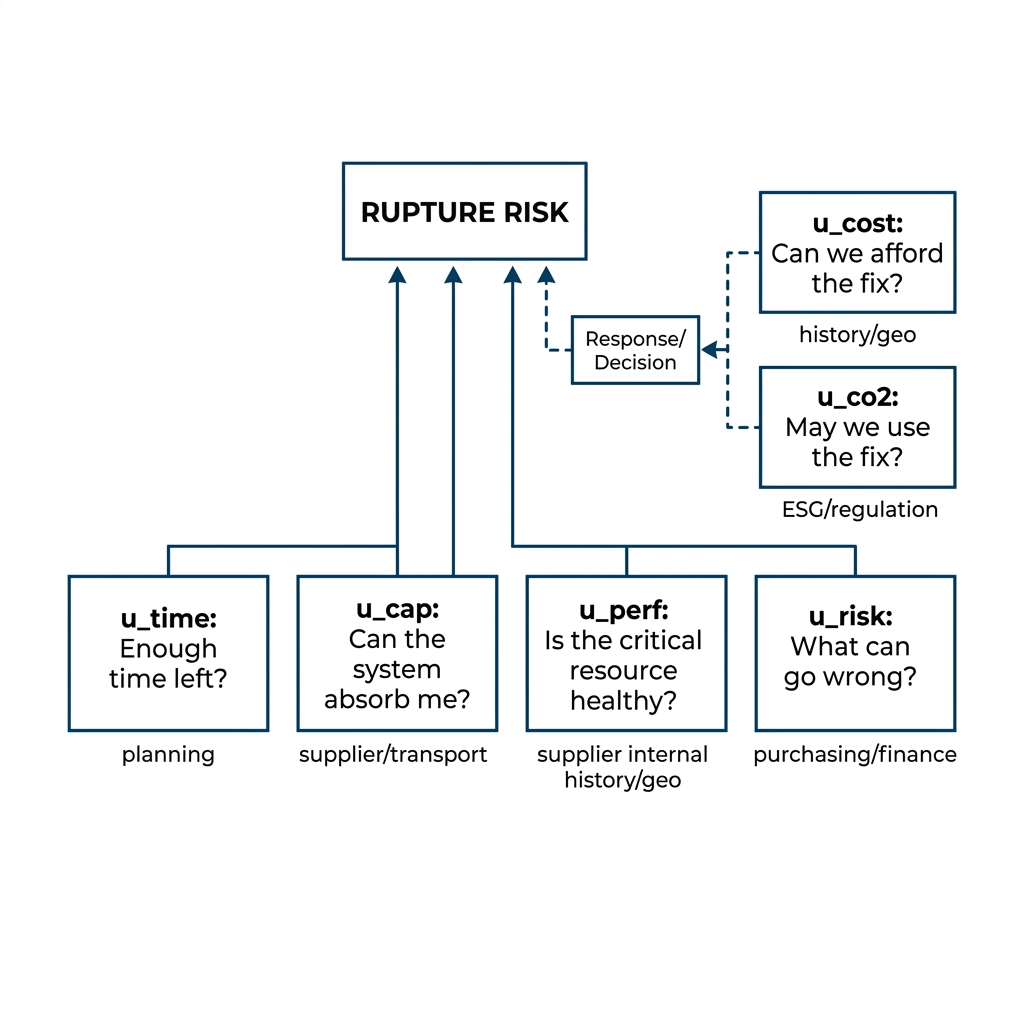
\includegraphics[width=0.82\linewidth]{Images/4.Operations/causal_tree_blocks.png}
    \caption{Causal structure behind the six-block selection}
    \label{fig:causal_tree_blocks}
\end{figure}

\subsubsection{Local Declared Urgency}
\label{sec:model_ud}

Symmetrically, declared urgency is not read as a single free-text estimate. It is
reconstructed from a structured elicitation so that it can be scored, propagated and
compared with $U_{r,\text{local}}$ on the same scale. At each node the operator compares
four criteria pairwise through the Analytic Hierarchy Process, which yields a
consistency-checked weight $w_j$ per criterion, then rates each criterion on a severity
scale $s_j \in \{1, \ldots, 9\}$. Local declared urgency is the weight-averaged severity
rescaled to $[0,1]$:

\begin{equation}
    U_{d,\text{local}} = \sum_{j=1}^{4} w_j\,\frac{s_j - 1}{8}, \qquad \sum_{j=1}^{4} w_j = 1.
    \label{eq:ud_local}
\end{equation}

The elicitation tool, its four criteria and the consistency gate that rejects an incoherent
weight vector are application choices described in Section~\ref{sec:ahp_tool}. What matters
here is that $U_{d,\text{local}}$ and $U_{r,\text{local}}$ are both bounded, node-local
quantities in $[0,1]$ before either is propagated.

\subsubsection{Network Propagation}
\label{sec:model_prop}

Declared urgency propagates downstream, from the final customer at rank~0 toward
raw-material suppliers, while real urgency propagates upstream, from suppliers toward the
final customer. Both use a leaky product rule that keeps the signals bounded in $[0,1]$ and
monotonically increasing as more neighbours become urgent:

\begin{align}
    U_{d,i} &= 1 - \bigl(1 - U_{d,\text{local},i}\bigr) \prod_{k \in \text{Succ}(i)}
    \bigl(1 - \gamma_{ik} U_{d,k}\bigr), \label{eq:ud_prop} \\
    U_{r,i} &= 1 - \bigl(1 - U_{r,\text{local},i}\bigr) \prod_{j \in \text{Pred}(i)}
    \bigl(1 - \beta_{ji} U_{r,j}\bigr), \label{eq:ur_prop}
\end{align}

where $\gamma_{ik} \in [0,1]$ is the downstream attenuation coefficient on arc $(i,k)$ and
$\beta_{ji} \in [0,1]$ the upstream amplification coefficient on arc $(j,i)$.
Table~\ref{tab:propagation_components} defines each term, and
Figure~\ref{fig:urgency_propagation} shows the two signals travelling in opposite directions
across the same graph. Backup arcs are documentary and inert with respect to both
propagations, a modelling choice that the campaign scenario exploits deliberately.

\begin{table}[htbp]
\centering
\caption{Terms of the propagation equations}
\label{tab:propagation_components}
\small
\begin{tabularx}{\linewidth}{llX}
\toprule
\textbf{Component} & \textbf{Type} & \textbf{Description} \\
\midrule
$U_{d,i}$, $U_{r,i}$ & Dependent variables & Propagated declared and real urgency at node
$i$ \\
$U_{d,\text{local},i}$, $U_{r,\text{local},i}$ & Input variables & Local urgency at node
$i$ after status-rule adjustment \\
$\gamma_{ik}$ & System parameter & Downstream demand attenuation coefficient on arc
$i \to k$ \\
$\beta_{ji}$ & System parameter & Upstream risk amplification coefficient on arc
$j \to i$ \\
$\text{Succ}(i)$, $\text{Pred}(i)$ & Structural sets & Nominal successors and predecessors
of node $i$ \\
\bottomrule
\end{tabularx}
\end{table}

\paragraph{When each quantity is computed.}
The weekly cadence governs when new data \emph{arrives}, not when the model runs, and the
two are easy to conflate. The sequence is as follows. A review submitted for one node writes
that node's KPI values and questionnaire answers. That write immediately triggers
recomputation of the node's own $u_m$ blocks and its two local quantities,
$U_{r,\text{local}}$ and $U_{d,\text{local}}$. The new local values then propagate, but only
along the directions that can be affected: a change in local real urgency is pushed through
the node's downstream cone toward the final customer, following
Equation~\ref{eq:ur_prop}, and a change in local declared urgency is pushed through its
upstream cone toward the suppliers, following Equation~\ref{eq:ud_prop}. Nodes outside those
two cones are not recomputed, because their values cannot have changed.

Two consequences matter for reading the results. Nothing is computed on a global weekly
timer, so the network is never in a state where all eight nodes were evaluated at the same
instant; a node reviewed on Monday and a node reviewed on Thursday hold values one review
apart, and the propagated figures reflect whatever the neighbours had most recently
submitted. And the campaign turn, not the calendar week, is the unit that makes the state
comparable across nodes, which is why every result in Section~\ref{sec:Results} is indexed by
turn.

\begin{figure}[htbp]
    \centering
    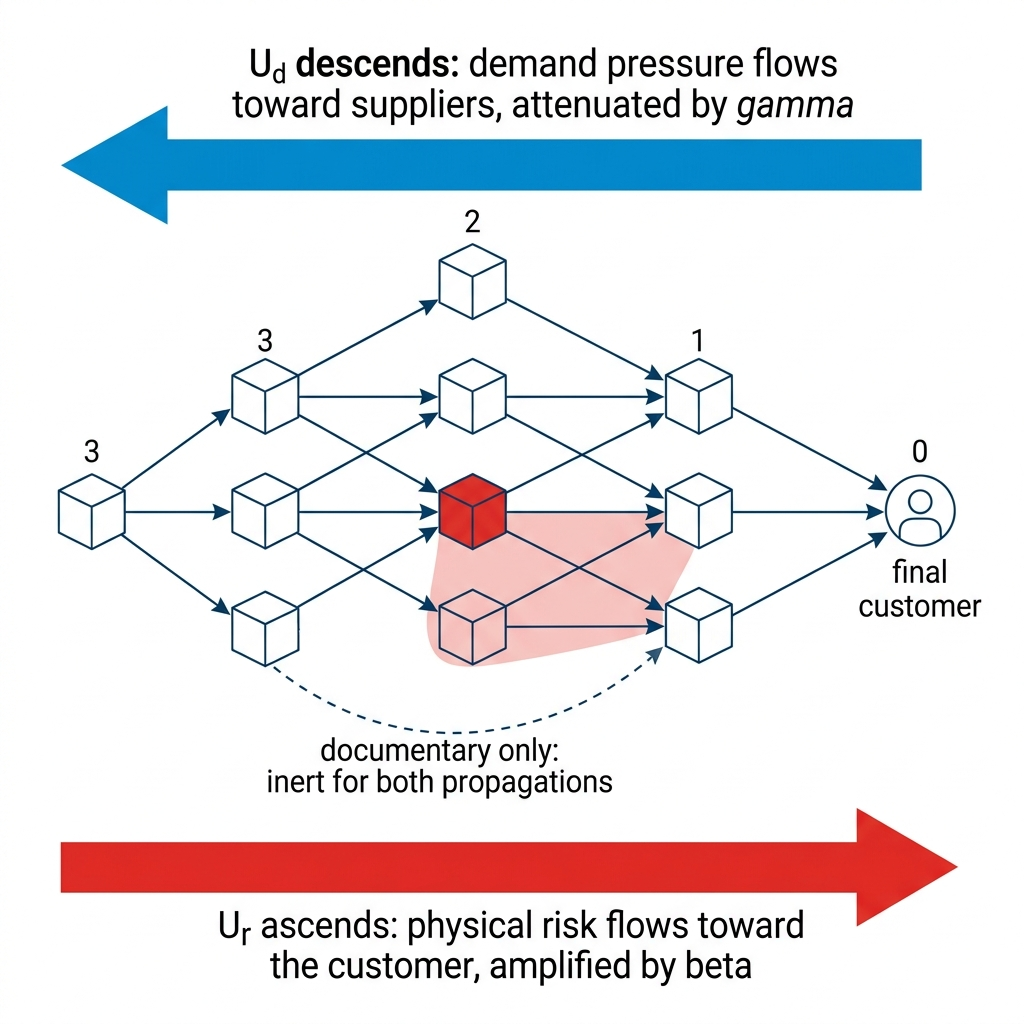
\includegraphics[width=0.82\linewidth]{Images/4.Operations/urgency_propagation.png}
    \caption{Bidirectional urgency propagation on the DAG}
    \label{fig:urgency_propagation}
\end{figure}

\subsubsection{Network Criticality Index}
\label{sec:criticality}

The criticality service answers one question systematically: which node, if it failed
completely, would cause the most damage to final-customer delivery? For every active node
in turn, the service forces the node's local real urgency to $1.0$, re-runs the ascending
propagation, and measures two deltas, the rise of $U_r$ at the final-customer nodes and the
largest rise anywhere in the network. Every shock is run twice, once on the standard
pipeline and once on an $\varepsilon$-regularised twin that carries the same propagation in
log-survival, $\ell(p) = -\ln(1-p)$, with urgency clipped to $1-\varepsilon$ so that a
survival product is never exactly zero. Nodes are ranked by the rise at the final customer
first, then by the corresponding log-survival delta $\Delta \ell_{\text{final}}$, then by
name. Figure~\ref{fig:shock_simulation} traces a single iteration of that sweep, from the
forced saturation of one node to the deltas it produces downstream.

One behaviour of this index matters for interpretation, and it is what the second sort key
exists for. A node already saturated at $U_r \ge 1.0$ yields a delta of zero and sinks to the
bottom of the ranking, since its risk is already realised in the baseline. In a network-wide
crisis, where many nodes saturate at once, $\Delta U_r$ collapses to zero throughout and the
ranking degenerates exactly where it would be most useful; nine of the nineteen campaign
turns are in that state, which is what the exclusion rule used by hypothesis H3 in
Section~\ref{sec:methods_campaign} was written for.

Because $\ell$ is strictly increasing, $\Delta \ell_{\text{final}}$ and the standard delta
at the final customer are two monotone transforms of the same shocked urgency, so outside
saturation they induce the same order and the ranking is unchanged. This is stated as a
property-based invariant and tested as one. Inside saturation the clip that flattens
$\Delta U_r$ does not flatten $\Delta \ell$, which continues to measure how much deeper a
shock drives an already saturated network. Section~\ref{sec:res_repair} reports what that
recovers on the campaign.

A second entry point answers the distributional question rather than the worst case. Instead
of forcing local urgency to $1.0$, it draws shock severities from the graduated flat-rate
severities of the calibrated event engine, minor, major and critical failures at $0.4$, $0.7$
and $1.0$ and financial alerts at $0.3$, $0.6$ and $0.9$, the two families weighted equally
and, within a family, by decreasing field frequency. Each draw is applied as a ratchet,
$\max(U_{r,\text{local}}, \text{severity})$, on the same principle as the event engine,
since a failure never improves a node's state. The batch is propagated in one vectorised
pass, in duplicate for both measures, and each node receives
$P(\Delta U_{r,\text{final}} > 0.2)$ together with the median and ninth decile of its
$\Delta \ell_{\text{final}}$ distribution. The computation is read-only, seeded and
deterministic.

\begin{figure}[htbp]
    \centering
    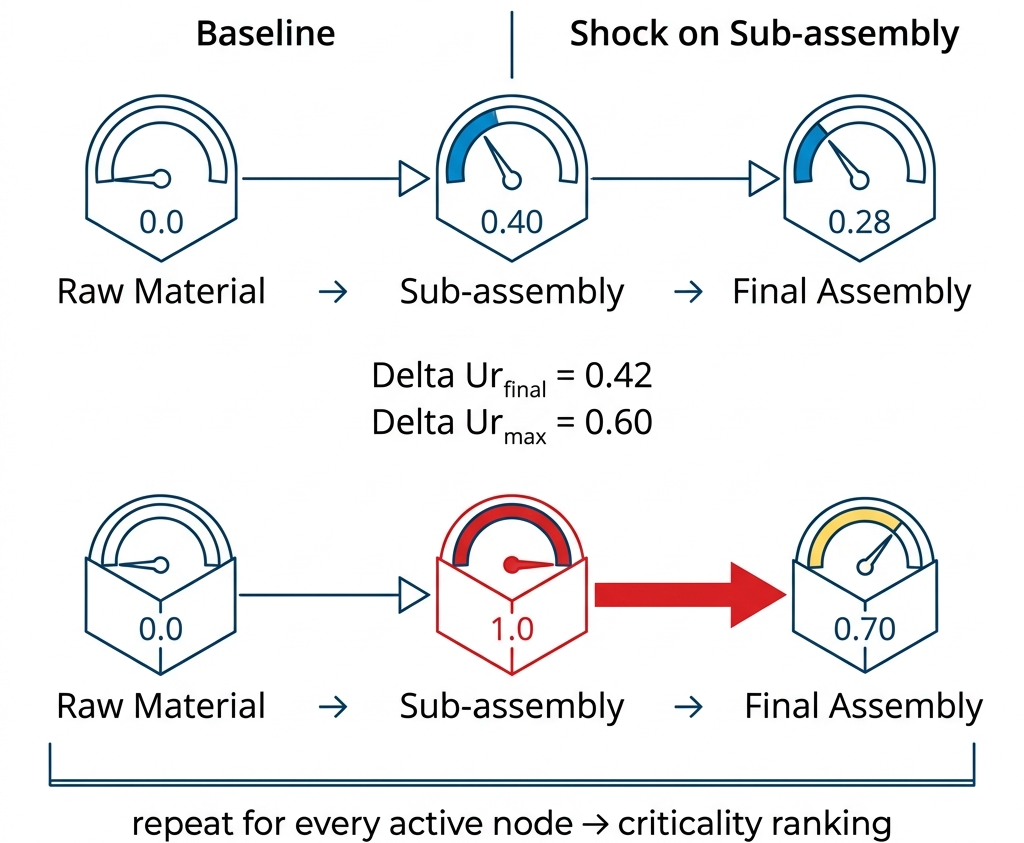
\includegraphics[width=0.82\linewidth]{Images/4.Operations/shock_simulation.png}
    \caption{One iteration of the shock simulation}
    \label{fig:shock_simulation}
\end{figure}

\subsubsection{Asymmetric Cognitive Adequacy}
\label{sec:model_adequacy}

The mismatch between declared and real urgency is split into two named pathologies, false
urgency $F$ for over-declaration and hidden risk $H$ for under-declaration:

\begin{equation}
    F = \max(U_d - U_r,\, 0), \qquad H = \max(U_r - U_d,\, 0).
    \label{eq:fh}
\end{equation}

Drawing on Prospect Theory~\autocite{kahneman1979prospect}, the two are penalised
asymmetrically and with diminishing marginal sensitivity to large errors:

\begin{equation}
    \text{penalty} = \lambda_{\text{under}} H^{\alpha} + \lambda_{\text{over}} F^{\alpha},
    \label{eq:penalty}
\end{equation}

and the penalty is rescaled into an adequacy score $A \in [0, 100]$ through an exponential
mapping bounded by the penalty of a maximal one-sided error, with each term defined in
Table~\ref{tab:adequation_components}:

\begin{equation}
    A = 100 \times \frac{\exp(-\text{penalty}) - \exp(-\text{penalty}_{\max})}
    {1 - \exp(-\text{penalty}_{\max})}, \qquad
    \text{penalty}_{\max} = \max(\lambda_{\text{under}}, \lambda_{\text{over}}).
    \label{eq:At}
\end{equation}

\begin{table}[htbp]
\centering
\caption{Terms and parameters of the adequacy equations}
\label{tab:adequation_components}
\small
\begin{tabularx}{\linewidth}{llXl}
\toprule
\textbf{Component} & \textbf{Type} & \textbf{Description} & \textbf{Default} \\
\midrule
$F$ & Dependent variable & False urgency, from over-declaration & n/a \\
$H$ & Dependent variable & Hidden risk, from under-declaration & n/a \\
$\lambda_{\text{under}}$ & System parameter & Penalty weight on hidden risk & $2.25$ \\
$\lambda_{\text{over}}$ & System parameter & Penalty weight on false urgency & $1.0$ \\
$\alpha$ & System parameter & Psychophysical curvature & $0.88$ \\
$A$ & Dependent variable & Adequacy score, $100$ meaning perfect alignment & $[0,100]$ \\
\bottomrule
\end{tabularx}
\end{table}

The governing constraint is $\lambda_{\text{under}} > \lambda_{\text{over}}$: a coordinator
who panics wastes premium transport capacity, but a coordinator who under-reports risk
misses the window to prevent a line stoppage, so under-declaration is priced more
expensively. The default ratio of $2.25$ reprises the loss-aversion coefficient, and
$\alpha = 0.88$ the curvature of the value function, both measured by
\textcite{kahneman1979prospect} and restated
later~\autocite{kahneman2011thinking}. These are literature-derived starting
points, not measured properties of supply chain coordinators. Both the aggregation weights
$\omega_m$ and the penalty parameters are configurable per project rather than hard-coded,
so recalibration requires no code change.

%% ═══════════════════════════════════════════════════════════════════════════
\subsection{System Implementation}
\label{sec:methods_impl}
%% ═══════════════════════════════════════════════════════════════════════════

The model above is deliberately silent on tooling. This section describes how each object
it defines is elicited from an operator, computed inside the running system, exposed back to
a coordinator and kept safe. The delivered system, SupplyScore, comprises 73 Python modules
across 10 packages, covered by 1\,779 automated test functions in 106 test files, including
property-based tests.

\subsubsection{Architecture}
\label{sec:architecture}

\paragraph{Single facade.}
All operations go through one orchestrating facade
(\texttt{services/}\allowbreak\texttt{orchestrator.py}) coordinating the mathematical core,
the graph repository and the persistence layers behind a single thread-safe entry point.
The web interface, the command-line entry point and the test suite all drive the system
exclusively through this facade, and there is no second write path.

\paragraph{Multi-tenant persistence.}
Data is split between one global registry database holding projects, nodes, arcs,
milestones and registry-level audit, and one SQLite database per node holding its private
operational history. This isolation prevents write contention between operators reviewing
different nodes and enforces the boundary that one supplier's raw history is not readable
through another supplier's records. It is also what makes the campaign of
Section~\ref{sec:methods_campaign} auditable per node after the fact.

\paragraph{Gatekeeper writes.}
Every business write crosses a single mutation service that whitelists the touched fields,
validates ranges, diffs against current state so that a no-op write leaves no trace, records
the change in the audit log with author and source, and synchronises the in-memory graph.
Audit tables are immutable, including from the administration interface.

\paragraph{Graph and propagation.}
The network lives in an in-memory graph repository backed by networkx. Propagation is
incremental, recomputing only the cones of nodes whose local urgency actually changed, which
keeps the twin responsive at the scale validated by dedicated performance benchmarks.
Figure~\ref{fig:uml_architecture} shows how the facade, the mutation gate and the two
persistence layers relate.

\paragraph{Decoupled clocks.}
Each project carries its own clock: a system clock for live use, a game clock advancing week
by week for serious-game sessions, and a fixed clock for deterministic tests. The weekly
cycle, milestone pressure and event timestamps all read the project clock rather than the
wall clock, which is what makes a compressed campaign possible without touching the model.

\begin{figure}[htbp]
    \centering
    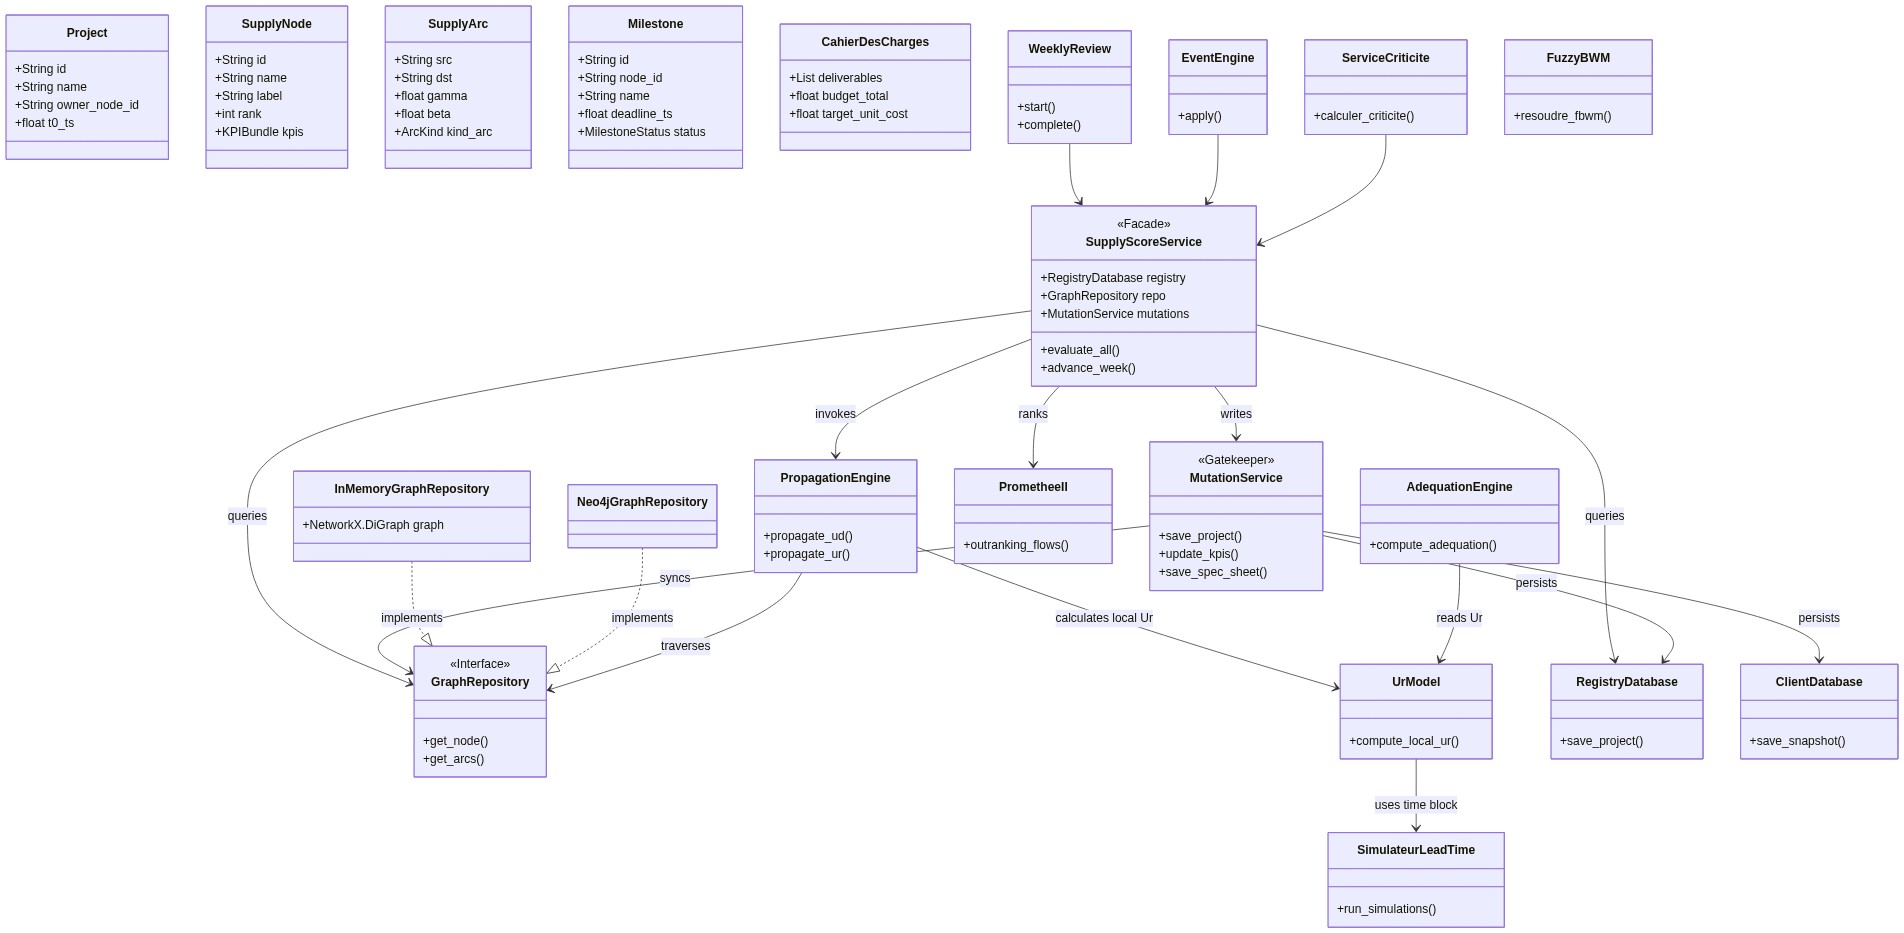
\includegraphics[width=0.78\linewidth]{Images/4.Operations/uml_architecture.png}
    \caption{The SupplyScore architecture}
    \label{fig:uml_architecture}
\end{figure}

\subsubsection{AHP Elicitation}
\label{sec:ahp_tool}

The module \texttt{core/ahp.py} implements the Saaty eigenvector method for a four-criterion
questionnaire administered through the weekly review page, and is the tool that produces
$U_{d,\text{local}}$. The four criteria are operational impact, meaning the downstream
consequence of failure; time window, meaning how long before the situation becomes
irredeemable; downstream dependencies, meaning how many tasks are blocked waiting; and
recoverability, meaning whether lateness can be caught up, inverted so that lower is worse.

The criteria set follows from two constraints. Cognitively, Saaty's method degrades as the
number of pairwise-compared criteria grows, with consistency hard to maintain beyond roughly
seven items and each additional criterion adding $n-1$ comparisons to the weekly
workload~\autocite{saaty1990how,triantaphyllou2024}. Keeping $n = 4$ limits the
questionnaire to six comparisons. Structurally, the four questions mirror how declared
urgency is consumed downstream: impact and dependencies capture the severity dimension that
propagation amplifies, the time window captures the slack dimension confronted with
$u_{\text{time}}$, and recoverability captures the resilience dimension confronted with the
recovery term of $u_{\text{risk}}$. Each declared criterion therefore has an operational
counterpart in the computed signal, which is what makes the later comparison meaningful
rather than a comparison of unrelated quantities. Figure~\ref{fig:ahp_criteria_mapping}
draws those four correspondences. Larger criteria sets are deliberately routed to the Fuzzy
BWM weighting of the KPI blocks instead.

The consistency ratio is computed as $\gls{cr} = \gls{ci} / \gls{ri}[n]$ using Saaty's
Random Index table. If $\gls{cr} > 0.10$ the interface flags the questionnaire as
inconsistent and invites the operator to revise the most contradictory comparison before the
assessment is accepted; Figure~\ref{fig:questionnaire} shows that gate in the interface.
Declared urgency is further smoothed with an exponential moving average, $\rho = 0.3$,
across consecutive weekly assessments, absorbing transient stress spikes without erasing a
sustained change in perception.

\begin{figure}[htbp]
    \centering
    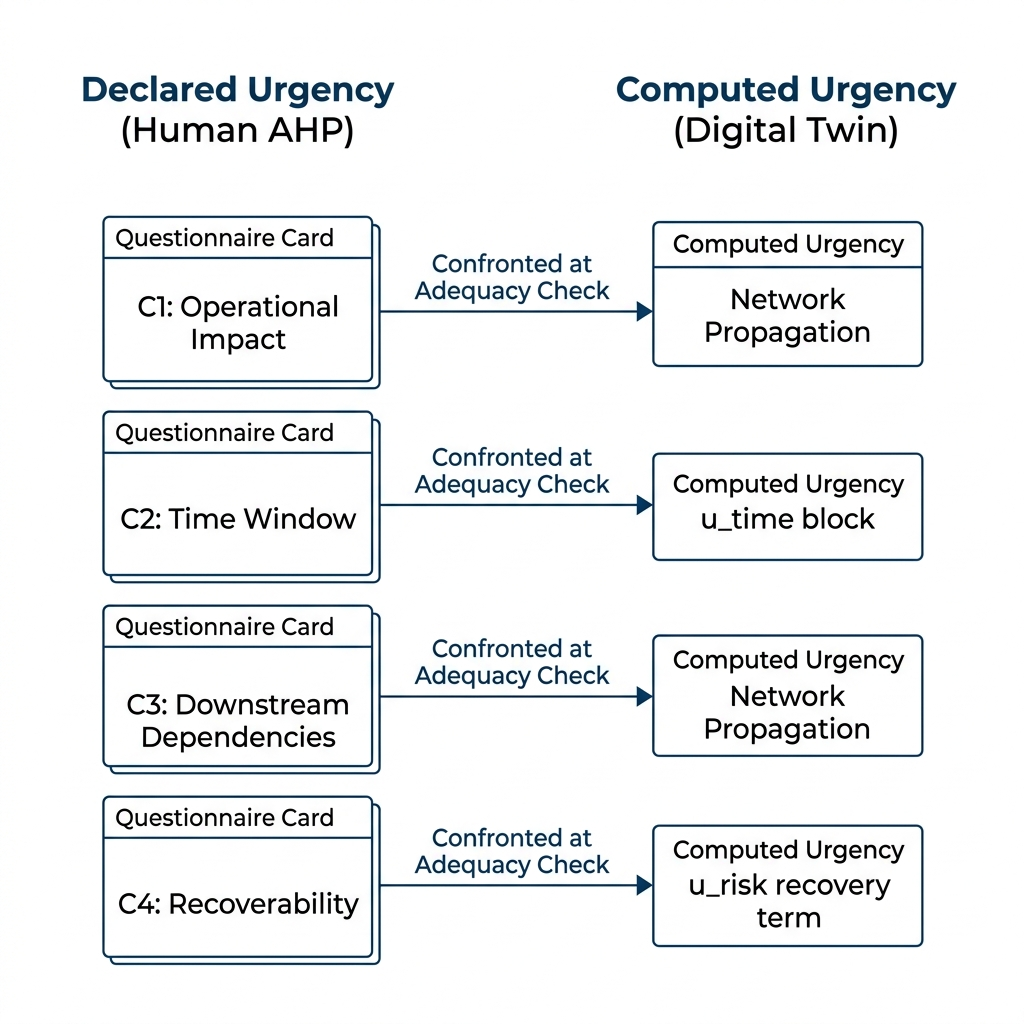
\includegraphics[width=0.82\linewidth]{Images/4.Operations/ahp_criteria_mapping.png}
    \caption{The four AHP criteria and their computed counterparts}
    \label{fig:ahp_criteria_mapping}
\end{figure}

\begin{figure}[htbp]
    \centering
    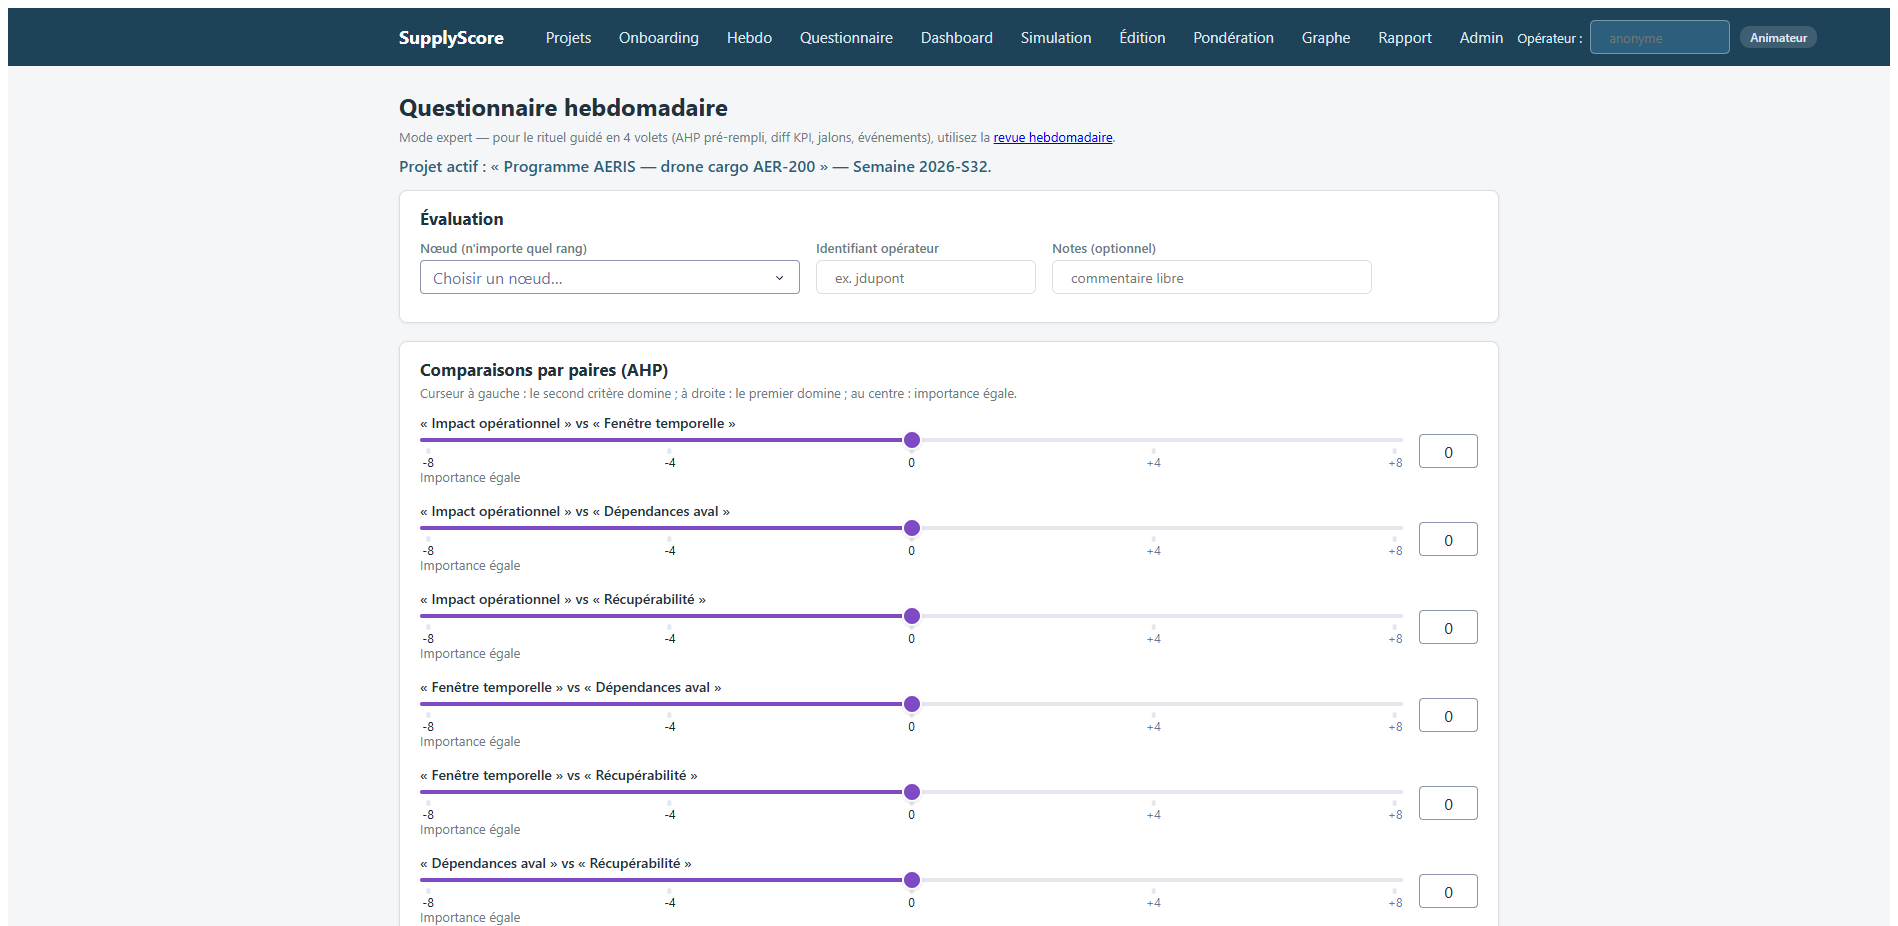
\includegraphics[width=0.78\linewidth]{Images/4.Operations/questionnaire_screenshot.png}
    \caption{The AHP questionnaire page}
    \label{fig:questionnaire}
\end{figure}

\subsubsection{Fuzzy BWM and PROMETHEE II Network Outranking}
\label{sec:fbwm_promethee}

The modules \texttt{mcda/fbwm.py} and \texttt{mcda/promethee.py} implement two complementary
methods. Fuzzy BWM offers a lower-effort elicitation route than crisp AHP for weighting the
six KPI blocks, and PROMETHEE~II turns those weights into a network-wide, non-compensatory
ranking of nodes.

The linguistic scale maps five qualitative judgements to triangular fuzzy numbers on a
1 to 4.5 scale, each carrying its own maximum consistency index. The consistency ratio is
$\gls{cr}_{\text{BWM}} = \xi^*/\text{CI}$, where $\xi^*$ is the optimal consistency
indicator returned by a constrained non-linear optimisation fitting the fuzzy weights to
the elicited comparisons. If the optimisation fails to converge, the implementation falls
back to uniform weights rather than raising an error, so a single malformed elicitation
cannot break the weekly review. Fuzzy weights are defuzzified with the Graded Mean
Integration Representation,

\begin{equation}
    w_j = \frac{a_j + 4 b_j + c_j}{6},
    \label{eq:bwm_defuzz}
\end{equation}

then renormalised to sum to one. The triangular bounds are written $(a_j, b_j, c_j)$ rather
than the more common $(l_j, m_j, u_j)$ to avoid colliding with the risk blocks $u_m$.

PROMETHEE~II ranks the active nodes of a project on the same six weighted urgency blocks
that feed local real urgency. For each pair of active nodes and each block, the preference
intensity is computed with a Type~V linear preference function with an indifference
threshold, and the aggregated preference index and net outranking flow follow the standard
formulation:

\begin{equation}
    \pi(a,b) = \sum_m \omega_m P_m\bigl(g_m(a) - g_m(b)\bigr), \qquad
    \phi(a) = \phi^+(a) - \phi^-(a).
    \label{eq:promethee_net}
\end{equation}

The same weights $\omega_m$ used in the local aggregation are reused as the PROMETHEE
criteria weights, so that the network ranking and the per-node urgency score remain mutually
consistent rather than relying on a separately calibrated weight set.

\subsubsection{Weekly Review Cycle and Calibrated Event Engine}
\label{sec:weekly_cycle}

The weekly review cycle keeps the twin's KPI state current without free-form manual data
entry: every write is structured, signed and auditable. At each new week every active node
is flagged as due for review, and the operator completes four sequential sections: the AHP
questionnaire, pre-filled with the previous week's values; the week's KPI values, shown
against the previous week; progress on active milestones, compared against theoretical
planning progress; and any supply chain events that occurred during the week. All four are
written as a single signed, atomic transaction, so no partial or anonymous review can
corrupt a node's history.

Rather than asking operators to recompute the KPI impact of a disruption by hand, the system
exposes a taxonomy of fourteen calibrated event types, each mapped to one or more KPI
updates through one of three calibration operators: a Beta-Bernoulli Bayesian update for
failure probabilities,

\begin{equation}
    p_{\text{post}} = \text{clip}\!\left(\frac{p\times n_0 + k}{n_0+n},\, 10^{-4},\,
    0.99\right),
    \label{eq:bayes_update}
\end{equation}

with a prior weight $n_0 = 26$, roughly six months of weekly observations; an exponential
moving average for continuous variables such as OEE,
$x_{\text{new}} = (1-\lambda)x_{\text{old}} + \lambda x_{\text{obs}}$ with
$\lambda \in [0.3, 0.5]$; and a ratchet update for severity,
$s_{\text{new}} = \max(s_{\text{old}}, s_{\text{event}})$.
Figure~\ref{fig:event_pipeline} follows one declared event through to the KPI fields it
revises, showing which of the three operators applies where.

\begin{figure}[htbp]
    \centering
    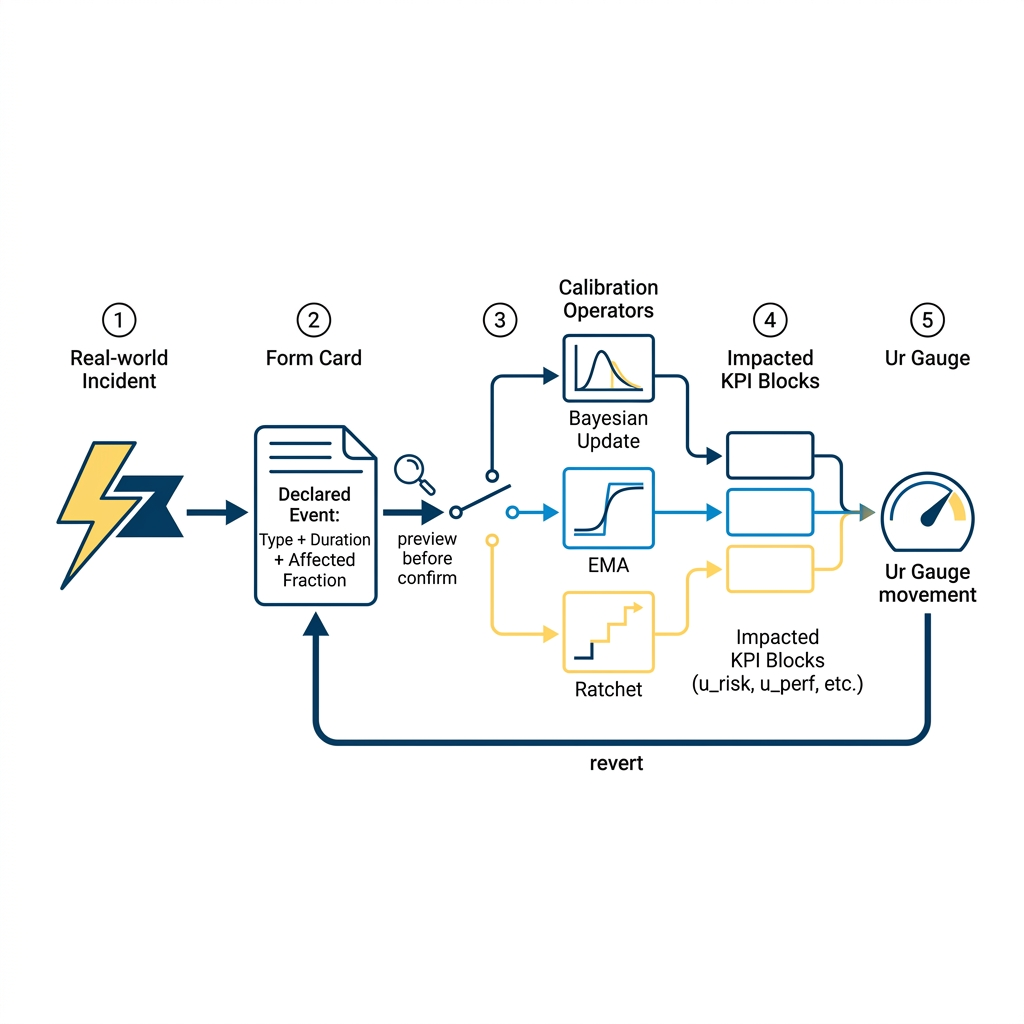
\includegraphics[width=0.82\linewidth]{Images/4.Operations/event_pipeline.png}
    \caption{From a declared event to a calibrated KPI update}
    \label{fig:event_pipeline}
\end{figure}

As a worked example, a node declaring a strike lasting $d = 24$ hours and affecting a
fraction $p_f = 0.50$ of the workforce implies $H_{\text{lost}} = d \times p_f = 12$
equivalent lost hours over a 168-hour week, so $f_{\text{lost}} \approx 0.0714$ and the
observed availability is $A_{\text{obs}} \approx 0.9286$. Updating a baseline availability
of $0.95$ with $\lambda = 0.5$ gives $A_{\text{new}} \approx 0.9393$, while risk severity
updates in ratchet mode to $\max(0.30, 0.50) = 0.50$.

\subsubsection{The Forecast Layer}
\label{sec:methods_forecast}

The results of this thesis turn on one component, so it is specified here rather than left
implicit behind the phrase used in the scoring protocol below. The forecast service projects
every active node over one to four weeks from that node's own persisted weekly history, and
emits the probability $p_h$ that an adverse outcome occurs within the horizon.

Three quantities are estimated from the history and then simulated forward. Local urgency is
extrapolated by a first-order autoregression fitted by least squares. The rate of adverse
events is a Beta posterior, the same conjugate revision the event engine uses. The lead time
is resolved to a distribution and resampled by parametric bootstrap. The rollout then draws a
node's future trajectory, and $p_h$ is the fraction of trajectories in which the outcome
occurs.

The estimator is deliberately tied to the target. What $p_h$ estimates is exactly the adverse
outcome of the calibration service, a missed milestone or a non-reverted event of gravity
critical or defect; the third condition of that definition, node abandonment, is not
simulated, because only active nodes are projected and abandonment is an outcome to
anticipate rather than an input state. The forecast is therefore the prospective estimator of
the quantity the calibration service measures retrospectively. Section~\ref{sec:res_target_trap}
shows how much rests on that alignment.

Uncertainty is decomposed rather than lumped. The simulation is nested: $K = 20$ outer draws
of the parameters themselves, the autoregression coefficient and residual scale through their
least-squares standard errors, the event rate through its Beta posterior and the lead-time
moments through the bootstrap, each carrying $n/K$ inner trajectories. The variance of $p_h$
splits into a Monte Carlo component within outer draws and a parametric component between
them, and the reported interval is labelled by the sources it covers. This matters for the
reliability analysis of Section~\ref{sec:res_armA_scored}, since an interval that hides which
uncertainty it represents cannot be read.

Two disciplines are enforced in the code rather than by convention. The service never writes,
so a forecast cannot perturb the state it forecasts. And counterfactual comparisons, which
price a corrective action by rerunning two branches on common random numbers, are named
throughout as an effect according to the model and never as a measured effect, because both
branches are simulated and neither is an observation.

\subsubsection{Explainability, Export and Operational Hardening}
\label{sec:explain_export}

When the twin flags a node, the coordinator's first question is why. The per-node
explanation page answers it with exact decompositions rather than approximations. Declared
urgency splits into one additive contribution per AHP criterion,
$\kappa_j = w_j (s_j-1)/8$, summing exactly to $U_{d,\text{local}}$. Local real urgency
splits the same way through the logarithm of Equation~\ref{eq:ur_local}: each block
contributes $\ell_m = -\omega_m\ln(1-u_m)$, the shares $c_m = \ell_m / \sum_k \ell_k$ sum to
one, and $U_{r,\text{local}} = 1-\exp(-\sum_m \ell_m)$ reconstructs the score exactly.
Figure~\ref{fig:explainability_waterfall} shows both decompositions side by side for a
single node. This matters for the results reported later, because it is what allows a score
to be traced back to the block that produced it without any manual computation.

One action compiles the global registry and per-node history into a twelve-worksheet Excel
workbook, so that analyses can run outside the tool on frozen data. The persistence layer
enables Write-Ahead Logging, runs an integrity check before every backup, and copies each
database through the native \texttt{sqlite3.backup} API without locking the running
application, with automatic backups every 24 hours and versioned schema migrations.

\begin{figure}[htbp]
    \centering
    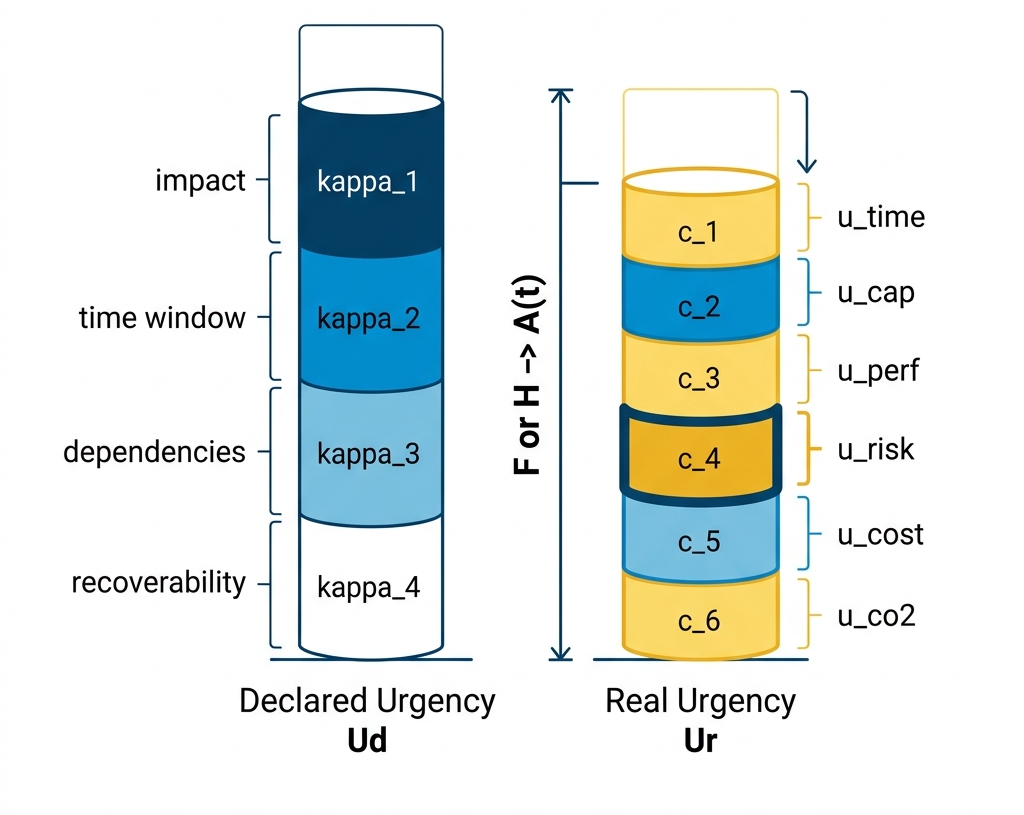
\includegraphics[width=0.78\linewidth]{Images/4.Operations/explainability_waterfall.png}
    \caption{Per-node explainability decomposition}
    \label{fig:explainability_waterfall}
\end{figure}

%% ═══════════════════════════════════════════════════════════════════════════
\subsection{Experimental Design: The H\'ELIOS Campaign}
\label{sec:methods_campaign}
%% ═══════════════════════════════════════════════════════════════════════════

Everything above establishes that the model is implemented, internally consistent and
tested. It does not establish whether the adequacy signal says anything true about an
operator facing a crisis. This section presents the experiment built for that purpose.

\subsubsection{Scenario and Network}
\label{sec:methods_scenario}

The campaign, presented to participants under the cover story \emph{Programme H\'ELIOS},
replays the 2020 to 2022 semiconductor shortage over eighteen weekly game turns plus a
training turn. The supply network has eight nodes, one per participant, anchored on the real
actor types of the crisis (Table~\ref{tab:helios_network}).

\begin{table}[htbp]
\centering
\caption{The eight H\'ELIOS campaign nodes}
\label{tab:helios_network}
\small
\begin{tabularx}{\linewidth}{>{\raggedright\arraybackslash}p{3.1cm} >{\raggedright\arraybackslash}p{2.6cm} c X}
\toprule
\textbf{Node} & \textbf{Role} & \textbf{Rank} & \textbf{Real-world anchor} \\
\midrule
Orbitalys & Satellite prime, final customer & 0 & Fictional satellite programme,
contractual delivery pressure \\
AvioSys Int\'egration & Avionics integrator & 1 & Qualified-stock squeeze on avionics
tier-1 suppliers \\
\'Electis EMS & Electronics manufacturing services & 2 & EMS plants placed under
allocation, 2021 \\
CompoDis Europe & Component distributor & 3 & Distributor allocation and spot-market
premiums \\
TransGlobal Fret & Freight operator & 3 & Suez Canal blockage, West Coast port
congestion \\
NovaFab Semiconductors & Foundry, expected bottleneck & 4 & Composite of the Texas
winter-storm freeze and the Taiwan drought \\
Meridian Semi & Secondary foundry, inert backup arc & 4 & A foundry sold out through 2023,
the announced plan B that delivers nothing \\
SilPure Materials & Raw wafer supplier & 5 & Roughly 60\% of world wafer supply,
polysilicon price roughly tripling in 2021 \\
\bottomrule
\end{tabularx}
\end{table}

Figure~\ref{fig:helios_network_coefficients} gives the network with its per-arc
coefficients, $\gamma$ attenuating demand as it descends and $\beta$ amplifying risk as it
ascends, together with each node's tier rank. NovaFab at rank 4 is the expected bottleneck.
The dashed arc into Meridian is the inert backup arc of Section~\ref{sec:model_prop}: it
appears in the diagram and carries nothing, which is the point of including it.

The turns follow five acts drawn from the documented chronology: a baseline where early
warning signs go unheeded, a tipping point where a foundry freeze, a competitor fire and a
canal blockage make the crisis visible, a squeeze where spot prices reach ten to forty times
catalogue, a rupture where a major manufacturer cuts production by roughly 40\% and the
announced backup foundry turns out to have no spare capacity, and a slow, partial recovery
that measures whether declared urgency lags the physical de-escalation. One game turn
represents one real month, with real durations converted into engine hours at a fixed rate
so that documented figures keep their true magnitude inside an eighteen-turn game.

\begin{figure}[htbp]
    \centering
    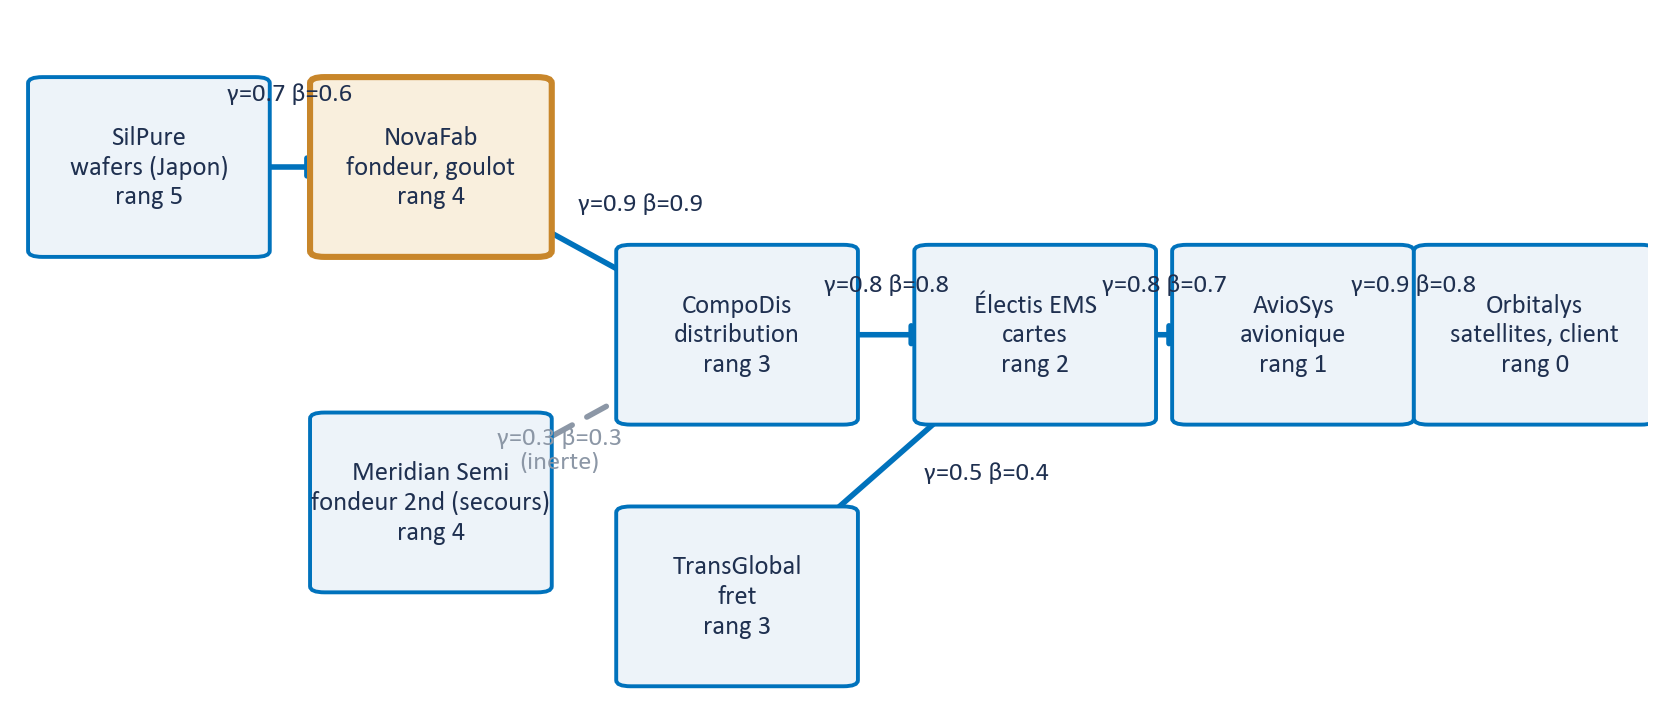
\includegraphics[width=\linewidth]{Images/4.Operations/helios_network_coefficients.png}
    \caption{The H\'ELIOS network and its per-arc coefficients}
    \label{fig:helios_network_coefficients}
\end{figure}

The twelve calibrated engine events driving the crisis are listed in
Table~\ref{tab:helios_events}, with the turn numbers as recorded in the campaign databases.
One encoding choice is worth noting: the Texas freeze is modelled as a production accident,
which triggers the engine's Bayesian revision of the failure probability, a recovery clock
and a severity ratchet, rather than as a capacity loss, which would only reduce storage
volume. A hot shutdown of a fabrication line is mechanically closer to the former.

\begin{table}[htbp]
\centering
\caption{The twelve calibrated engine events}
\label{tab:helios_events}
\small
\begin{tabularx}{\linewidth}{c >{\raggedright\arraybackslash}p{2.3cm} >{\raggedright\arraybackslash}p{2.9cm} X}
\toprule
\textbf{Turn} & \textbf{Node} & \textbf{Event type} & \textbf{Real-world anchor} \\
\midrule
T3 & NovaFab & Demand spike & Automotive reorders on sold-out slots, Nov.\ 2020 \\
T5 & CompoDis & Supplier delay & Distributor moves to allocation, Jan.\ 2021 \\
T6 & NovaFab & Accident (critical) & Texas winter-storm fab freeze, Feb.\ 2021 \\
T7 & NovaFab & Demand spike & Reorders after a competitor's fab fire, Mar.\ 2021 \\
T7 & TransGlobal & Transport disruption & Suez Canal blockage, six days, Mar.\ 2021 \\
T10 & NovaFab & Material shortage & Taiwan drought, ultrapure-water rationing, Jun.\ 2021 \\
T12 & \'Electis & Capacity loss & Southeast-Asia backend lockdowns, Aug.\ 2021 \\
T12 & TransGlobal & Transport disruption & Shift to saturated air freight, Aug.\ 2021 \\
T13 & CompoDis & Demand spike & Bullwhip over-ordering, Sep.\ 2021 \\
T14 & TransGlobal & Transport disruption & West Coast port congestion, Oct.\ 2021 \\
T14 & CompoDis & Tariff increase & Allocation spot premiums, Oct.\ 2021 \\
T16 & SilPure & Tariff increase & Polysilicon price pass-through, Dec.\ 2021 \\
\bottomrule
\end{tabularx}
\end{table}

\subsubsection{Data Provenance}
\label{sec:methods_data}

The two urgency signals come from different sources, which is the point of the design. Real
urgency is fed from public time series of the actual crisis, namely INSEE production and
price indices, WSTS worldwide semiconductor billings and a semiconductor-shortage dataset,
frozen in a data pack whose SHA-256 hashes were recorded before the first turn. Declared
urgency comes from the participants through the weekly AHP questionnaire, with the
consistency gate active.

Every third-party dataset is passed through an authenticity check before use. A logistics
dataset initially considered for the freight node was rejected at this check for the
signatures of synthetic training data, namely pre-computed target columns, GPS coordinates
scattered outside the region the dataset claimed to cover, and uniformly flat
distributions. The semiconductor-shortage dataset passed, showing a secular price decline, a
genuine 2021 upturn and sectoral employment consistent with official series. The rejected
dataset is retained in the raw-data folder for audit but is never loaded by the analysis
pipeline, and the freight node's cost block is driven entirely by calibrated events instead.

Two provenance rules protect the real-urgency series. A single-pilot rule forbids double
counting: each KPI field of each node is driven either by a time series or by a calibrated
event, never by both, so when an event writes a field on a given turn the series skips that
turn. Second, one honest artefact of the real data is kept rather than smoothed away. The
INSEE business-failures series falls through 2020 and 2021 under public support schemes, so
a failure-rate indicator taken alone would lower external risk exactly while the sector
crisis was worsening. Keeping it makes the multi-block argument concrete: a single
macroeconomic indicator can tell the opposite of the ground truth.

\subsubsection{The Three Arms}
\label{sec:methods_arms}

The experiment compares three arms on the same frozen scenario. The comparison is what
allows the effect of a treatment to be separated from the behaviour of the scenario.

\begin{description}
    \item[Arm A, blind declaration.] Eight isolated agents declare their urgency each turn
    seeing only their own role card and turn briefing. No forecast is shown. This is the
    control condition and the source of the prospective forecasts that are scored in
    Section~\ref{sec:res_armA_scored}.
    \item[Arm B, forecast-assisted declaration.] The same agents, the same frozen scenario,
    but from turn 4 onward each agent is additionally shown the predictive analysis of its
    own node before declaring. The loop is open: nothing changes in the terrain, the
    scenario stays frozen, so the forecasts remain scorable and the effect of the treatment
    is measured on perception alone. Each declaration additionally records an
    \texttt{influence\_prediction} field taking one of four values, meaning no influence,
    confirms my assessment, revised upward, or revised downward. That field is the direct
    measure of the treatment effect.
    \item[Arm C, closed loop.] The agents act on the terrain through a catalogue of
    interventions applied by the mutation service and recorded in an intervention journal, so
    the ground truth itself changes. Arm C was executed in its agent version after the repair
    of Section~\ref{sec:res_repair}, over the same nineteen turns; because action destroys the
    reference truth, it is judged by comparing its final state with arm A rather than by
    scoring its forecasts.
\end{description}

The distinction between B and C is one of nature rather than degree. In arm B the ground
truth is fixed, so the predictions are scorable with proper scoring rules and the treatment
effect is measured on perception. In arm C, action destroys the reference truth, because a
rupture avoided thanks to an alert makes a good prediction look wrong, so arm C can only be
judged by comparing its final state with arm A. That comparison is reported in
Section~\ref{sec:res_repair}, and it is why the headline count of unfinished milestones is
not the figure to read.

Two properties of this design are worth stating explicitly, because the results depend on
them. First, the agents are language models, one per role, each confined to its own role
card and turn briefings with no access to the other roles, the dashboard or future turns.
This anti-lookahead discipline is enforced by the harness rather than by instruction. A
single model instance per role has no statistical standing as a substitute for eight
independent human judges, and Section~\ref{sec:res_discussion} treats that as the principal
threat to external validity. Second, the declaration format in arm B is identical to arm A,
which is what makes the two comparable, with the single addition of the influence field.

\subsubsection{Scoring Protocol}
\label{sec:methods_scoring}

The forecast layer emits, for each node and each turn from turn 4 onward, a probability
$p_h$ that an adverse outcome occurs at horizons $h \in \{1,2,3,4\}$ weeks. Scoring those
forecasts requires an outcome definition, and this thesis uses the one the production
calibration service itself applies, so that the model is judged against the target it was
built for. A node-week is a positive observation when at least one of three conditions holds
within the window $[S+1, S+h]$: a milestone of the node whose deadline falls in the window
is abandoned or is still active with its deadline passed; the node is abandoned; or an event
of gravity critical or defect is recorded and not subsequently reverted.

Four quantities are computed, following standard forecast verification
practice~\autocite{brier1950verification,murphy1973vector,gneiting2007strictly}:

\begin{itemize}
    \item \textbf{Discrimination}, by the area under the ROC curve, computed by mean ranks
    so that tied forecasts are handled correctly, with a percentile bootstrap 95\% interval
    over 2\,000 resamples. AUC answers whether the forecast orders node-weeks correctly.
    \item \textbf{Calibration}, by the Brier score and its skill against the climatological
    forecast that always announces the base rate. A negative skill means the forecast is
    worse calibrated than announcing the base rate.
    \item \textbf{Reliability}, by a banded table comparing the mean announced probability
    with the observed frequency in each band. The bands are deliberately uneven, because a
    uniform ten-bin split hides the failure mode that matters here.
    \item \textbf{Operating point}, by the confusion matrix at the pre-registered threshold
    of $0.5$ used by hypothesis H4.
\end{itemize}

Separating discrimination from calibration is essential rather than
decorative~\autocite{murphy1973vector}: a forecast can order outcomes correctly while
announcing the wrong probabilities, and the two failures call for different remedies.
Section~\ref{sec:res_armA_scored} finds exactly that dissociation.

One further check is built into the protocol. Because the outcome definition is a modelling
choice rather than a given, the same forecasts are additionally scored against a
deliberately naive target, namely any non-reverted event on the node regardless of gravity
and ignoring milestones. The difference between the two scorings is reported in
Section~\ref{sec:res_target_trap} and is treated as a result in its own right.

\subsubsection{Protocol Integrity and Controls}
\label{sec:methods_controls}

The protocol was frozen before the first turn. Participants see only their own role sheet
and questionnaire; dashboards and scores stay hidden until the debrief, and no discussion
between roles is allowed. Two placebo sheets, a false de-escalation handed to one node at
turn 9 and to another at turn 15, control for suggestibility: if a declared urgency follows
the placebo, the measure is reflecting the sheet handed over rather than a reading of the
situation. A weak-signal turn, where the press mentions a tension with no engine event
behind it, measures who reacts to media noise alone. Roles are assigned so that the two most
information-heavy nodes do not go to the most experienced participants, keeping a role
effect from being confounded with an expertise effect. Every deviation from protocol is
logged the same day in a campaign journal, and any analysis outside the pre-registered
hypothesis register of Section~\ref{sec:hypotheses} is labelled exploratory.

%% ═══════════════════════════════════════════════════════════════════════════
\subsection{Limitations and Simplifications of the Method}
\label{sec:methods_limits}
%% ═══════════════════════════════════════════════════════════════════════════

Four simplifications are built into the method itself, as distinct from the limitations of
the delivered framework catalogued in Section~\ref{sec:limitations}.

The six KPI blocks are treated as probabilistically independent so that the noisy-OR
aggregation is admissible. They are not independent in reality: a capacity loss raises cost,
and a performance drop lengthens lead time. The consequence is that correlated blocks
double-count evidence, which the composite-indicator literature identifies as the standard
failure mode of weighted aggregation~\autocite{greco2018,becker2017}. The explainability
decomposition of Section~\ref{sec:explain_export} is the mitigation: the coordinator sees
per-block contributions rather than only the aggregate, so a correlation is visible rather
than hidden.

The network is assumed acyclic, which permits a linear topological sort and makes
propagation deterministic and cheap. Real supply networks contain feedback, most obviously
in returns and rework loops.

The scenario is scripted, which is what makes the ground truth knowable and the forecasts
scorable, but it also means the events are the only source of adverse outcomes. The
consequence, quantified in Section~\ref{sec:res_armA_scored}, is that the positive class is
extremely small, and any conclusion about discrimination is correspondingly weak.

The declarants are language models. This buys perfect protocol compliance, exact
reproducibility and no scheduling cost, and it loses the property that matters most for
hypothesis H4, namely a genuinely imperfect human perception of a crisis. This is discussed
at length in Section~\ref{sec:res_discussion} rather than treated as a detail.

%% ═══════════════════════════════════════════════════════════════════════════
\subsection{Reproducibility}
\label{sec:methods_repro}
%% ═══════════════════════════════════════════════════════════════════════════

Every numerical result in Section~\ref{sec:Results} is regenerated from raw artifacts by a
single script, \texttt{Utilities/figures/derive.py}, which writes a JSON file that both the
figures and the text of this thesis read. No number in this document is transcribed by hand
from an intermediate report.

The inputs to that script are the two campaign databases, one per arm, and the raw
per-agent declaration and forecast logs. The outcome labels are not reimplemented: the
script calls the production \texttt{CalibrationService} directly, so the thesis scores the
model against the same target definition the running system applies. Random procedures are
seeded, specifically the bootstrap interval on the AUC and the Monte Carlo lead-time
simulation.

Two provisions guard against silent drift. The script recomputes the arm A against arm B
forecast comparison on every run and reports whether the two arms carry identical
prediction-layer output, which they must, since the replay is deterministic and only the
declarations differ. It also reports the outcome base rate at every horizon, so that a
change in the underlying database would be visible immediately rather than absorbed into a
summary statistic.

One earlier analysis file in the campaign folder, \texttt{analysis/rapport\_experience.md}
with its companion JSON, contains a superseded run whose participant-influence counts
disagree with the raw logs. It is deliberately not used anywhere in this thesis, and the
derivation script names it in an exclusion list so that the choice is recorded in the output
rather than left implicit.

The satellite observation system of Section~\ref{sec:res_volume} is a separate codebase with
its own verification script. Its network calls are cached on disk, so a re-run does not
depend on the availability of the public services it draws from, and its calibrated
constants are stated in the source with the sample size behind each.

%% ═══════════════════════════════════════════════════════════════════════════
\subsection{Ethical Considerations}
\label{sec:methods_ethics}
%% ═══════════════════════════════════════════════════════════════════════════

The research was conducted under the Cranfield University Research Ethics System. The study
as executed involves no human participants: the eight declarants are language-model agents,
and no personal data was collected, processed or stored at any point. The approval
documentation is reproduced in Appendix~\ref{app:ethics}.

The protocol was originally designed for eight human consultants, and that version would
have required participant consent for two specific features. The first is the cover story:
participants would be told they are playing a fictional satellite programme without being
told that the scenario replays a documented historical crisis, since knowing it would
destroy the measure. The second is the two placebo sheets, which deliberately hand a
participant false information. Both are standard incomplete-disclosure designs and both
would be resolved by a full debrief at the end of the campaign, in which the real scenario
is revealed and each participant is asked at which turn they recognised it. Were that
campaign to be run, informed consent, the right to withdraw, and the debrief would need to
be in place before the first turn.

Two further considerations apply to the work as it stands. The industrial data behind
the scenario is public, namely INSEE and WSTS series and an open dataset, and the commercial
material belonging to ALTEN is covered by the confidentiality statement at the front of this
thesis. For the satellite observation work, all imagery and building data come from public
French open-data services under their published licences, no imagery of private individuals
is collected or retained, and the analysis operates on industrial buildings rather than on
people. The regulatory database used there serves only to calibrate a constant and is never
used to infer a result about a specific site, which is a deliberate constraint rather than
an incidental property.

%% ═══════════════════════════════════════════════════════════════════════════
\subsection{Conclusion}
\label{sec:methods_conclusion}
%% ═══════════════════════════════════════════════════════════════════════════

The method combines a probabilistic multi-block urgency model, a structured elicitation of
declared urgency, a bidirectional propagation over the supply network, and an asymmetric
scoring of the mismatch between the two, implemented as a tested, auditable and persistent
system. Around that system, a pre-registered three-arm experiment on a frozen historical
scenario allows the resulting forecast to be scored against recorded outcomes with proper
scoring rules, and allows the effect of showing that forecast to the declarant to be
isolated from the behaviour of the scenario itself.

What this method can establish is bounded by its own design, and those bounds have been
stated rather than left implicit. Section~\ref{sec:Results} reports what it measured.


\clearpage
\section{Results and Discussion}
\label{sec:Results}
%% ═══════════════════════════════════════════════════════════════════════════
\subsection{Introduction}
\label{sec:res_intro}
%% ═══════════════════════════════════════════════════════════════════════════

Two claims are worth separating before any figure is given, because conflating them is the
easiest way to misread what follows. That the gap between declared and computed urgency
carries information about which supplier will fail is supported by the campaign. That the gap
can be converted into a well-calibrated probability attached to a named week is not, yet. The
distance between those two statements is the subject of
Sections~\ref{sec:res_armA_scored} and~\ref{sec:res_repair}, and the sample that bounds both
is stated wherever a figure is given.

Every number below is regenerated from raw artefacts by the derivation script described in
Section~\ref{sec:methods_repro}.

%% ═══════════════════════════════════════════════════════════════════════════
\subsection{The Delivered System}
\label{sec:res_system}
%% ═══════════════════════════════════════════════════════════════════════════

SupplyScore is delivered as a standalone Python application: 73 modules across 10 packages,
covered by 1\,831 automated test functions in 106 test files, driving a multi-page Dash web
interface over a multi-tenant SQLite persistence layer. The suite expands to 2\,044 collected
cases, of which 2\,028 pass and 15 are skipped for want of an optional dependency; one fails
on two missing image files referenced by a presentation script outside the library. All of the mathematical objects of
Section~\ref{sec:math_framework} are implemented and exercised: the six-block noisy-OR
aggregation, the AHP elicitation with its consistency gate, the Fuzzy BWM weighting, the
bidirectional DAG propagation, the asymmetric adequacy score, the Monte Carlo lead-time
estimate, the PROMETHEE~II network outranking and the systematic shock-simulation
criticality index.

Three operational capabilities carry what follows. The per-node explainability page
reconstructs any score term by term, which is what allowed the diagnosis in
Section~\ref{sec:res_mechanism} to be made from the application rather than by hand. The Excel
export produces frozen data for analysis outside the tool. And the hardened persistence layer
is what makes a campaign database an auditable record weeks after the run. Two pages carry
most of the operator's interaction with the system: the weekly review
(Figure~\ref{fig:hebdo}) and the criticality ranking (Figure~\ref{fig:criticite}).

\begin{figure}[htbp]
    \centering
    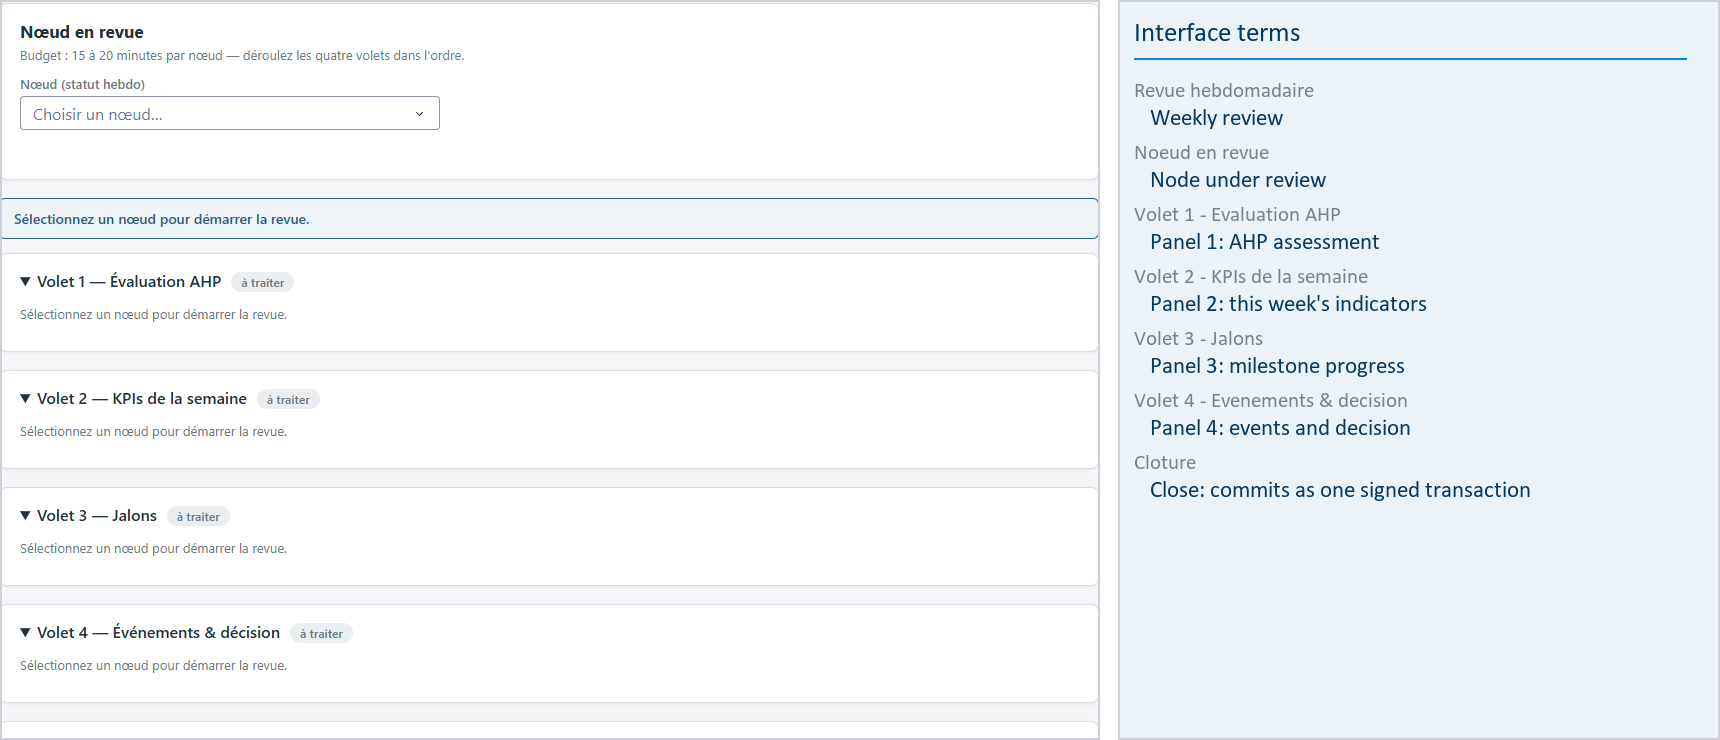
\includegraphics[width=\linewidth]{Images/4.Operations/weekly_review_annotated.png}
    \caption[The weekly review page]{The weekly review page, with its interface terms keyed
    into English. The four panels commit as one signed transaction.}
    \label{fig:hebdo}
\end{figure}

\begin{figure}[htbp]
    \centering
    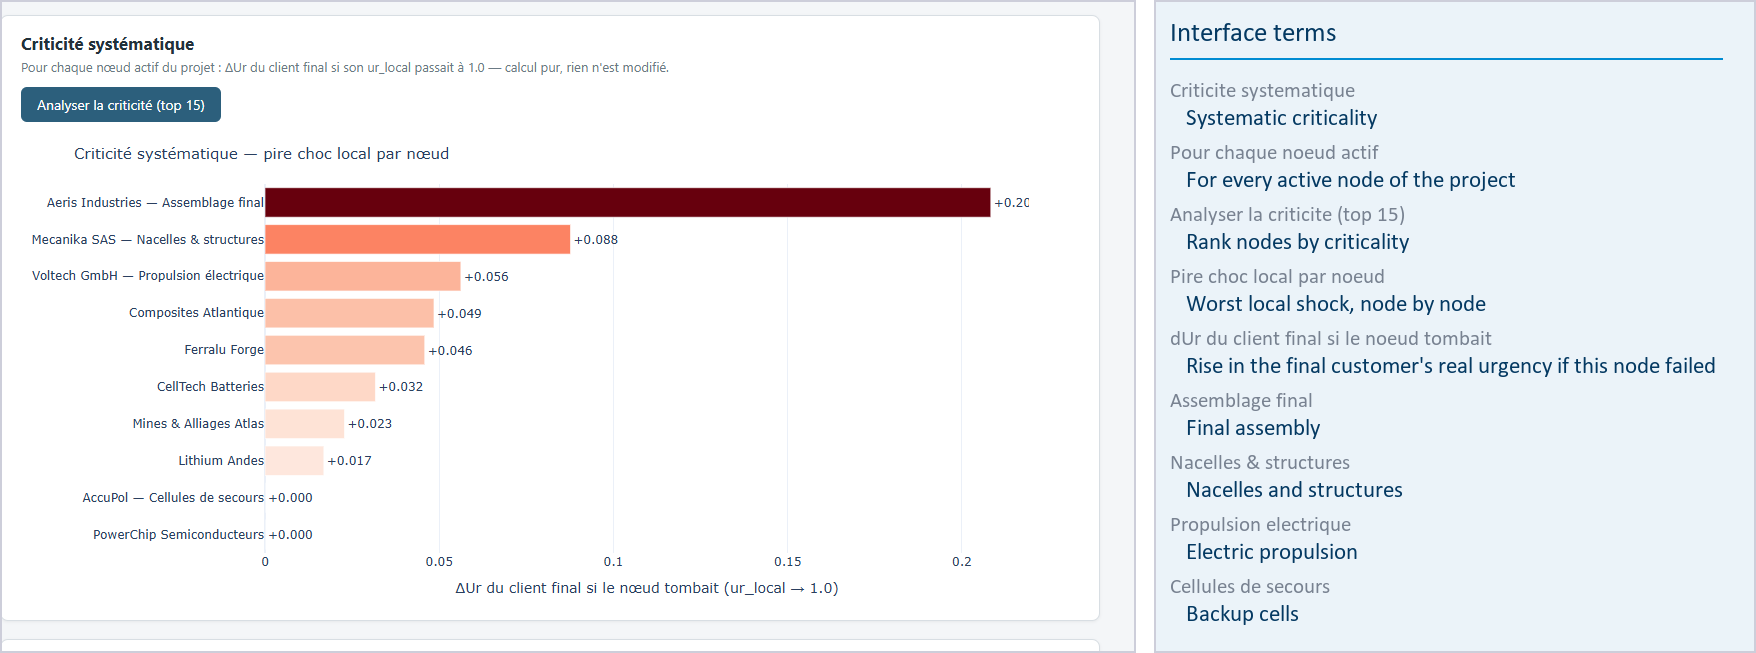
\includegraphics[width=\linewidth]{Images/4.Operations/criticality_annotated.png}
    \caption[Network criticality ranking]{The criticality ranking a coordinator would use to
    decide where to look first: for each active node, the rise in the final customer's real
    urgency were that node to fail completely.}
    \label{fig:criticite}
\end{figure}

%% ═══════════════════════════════════════════════════════════════════════════
\subsection{Mechanical Validation: The Synthetic Dry Run}
\label{sec:res_dryrun}
%% ═══════════════════════════════════════════════════════════════════════════

Before any declaration data existed, the full campaign mechanics were exercised end to end on
a disposable database. Five iterations calibrated the scenario and eliminated engine
artefacts, and the final iteration replayed all nineteen turns with synthetic respondents
standing in for the eight declarants.

This is an engineering check, not a scientific one, and the reason is in how the synthetic
declarations were made: each is anchored on the node's own local real urgency, following
$1 + 8 \times U_{r,\text{local}}$ with a fixed panic, under-report or neutral bias per role. A
declaration built that way cannot lag the signal it is derived from, cannot under-report it
for long, and cannot react at all to a press event it never reads, so it returns not confirmed
or not applicable on all six hypotheses by construction.
Figure~\ref{fig:helios_dryrun_trajectories} shows that circularity: real urgency solid and
synthetic declared urgency dashed, tracking each other closely at every node rather than one
lagging or decoupling from the other.

What the run does establish is that injection, weekly decay, milestone drift, event
calibration, propagation, criticality, snapshotting and backup all run correctly under the
two-turns-per-day cadence the campaign requires. It also calibrated the null baseline
detector, a raw threshold $U_{r,\text{local}} \ge 0.5$, at precision $0.16$ and recall
$0.27$: the bar the adequacy signal must clear to demonstrate value beyond a raw KPI
reading.

\begin{figure}[htbp]
    \centering
    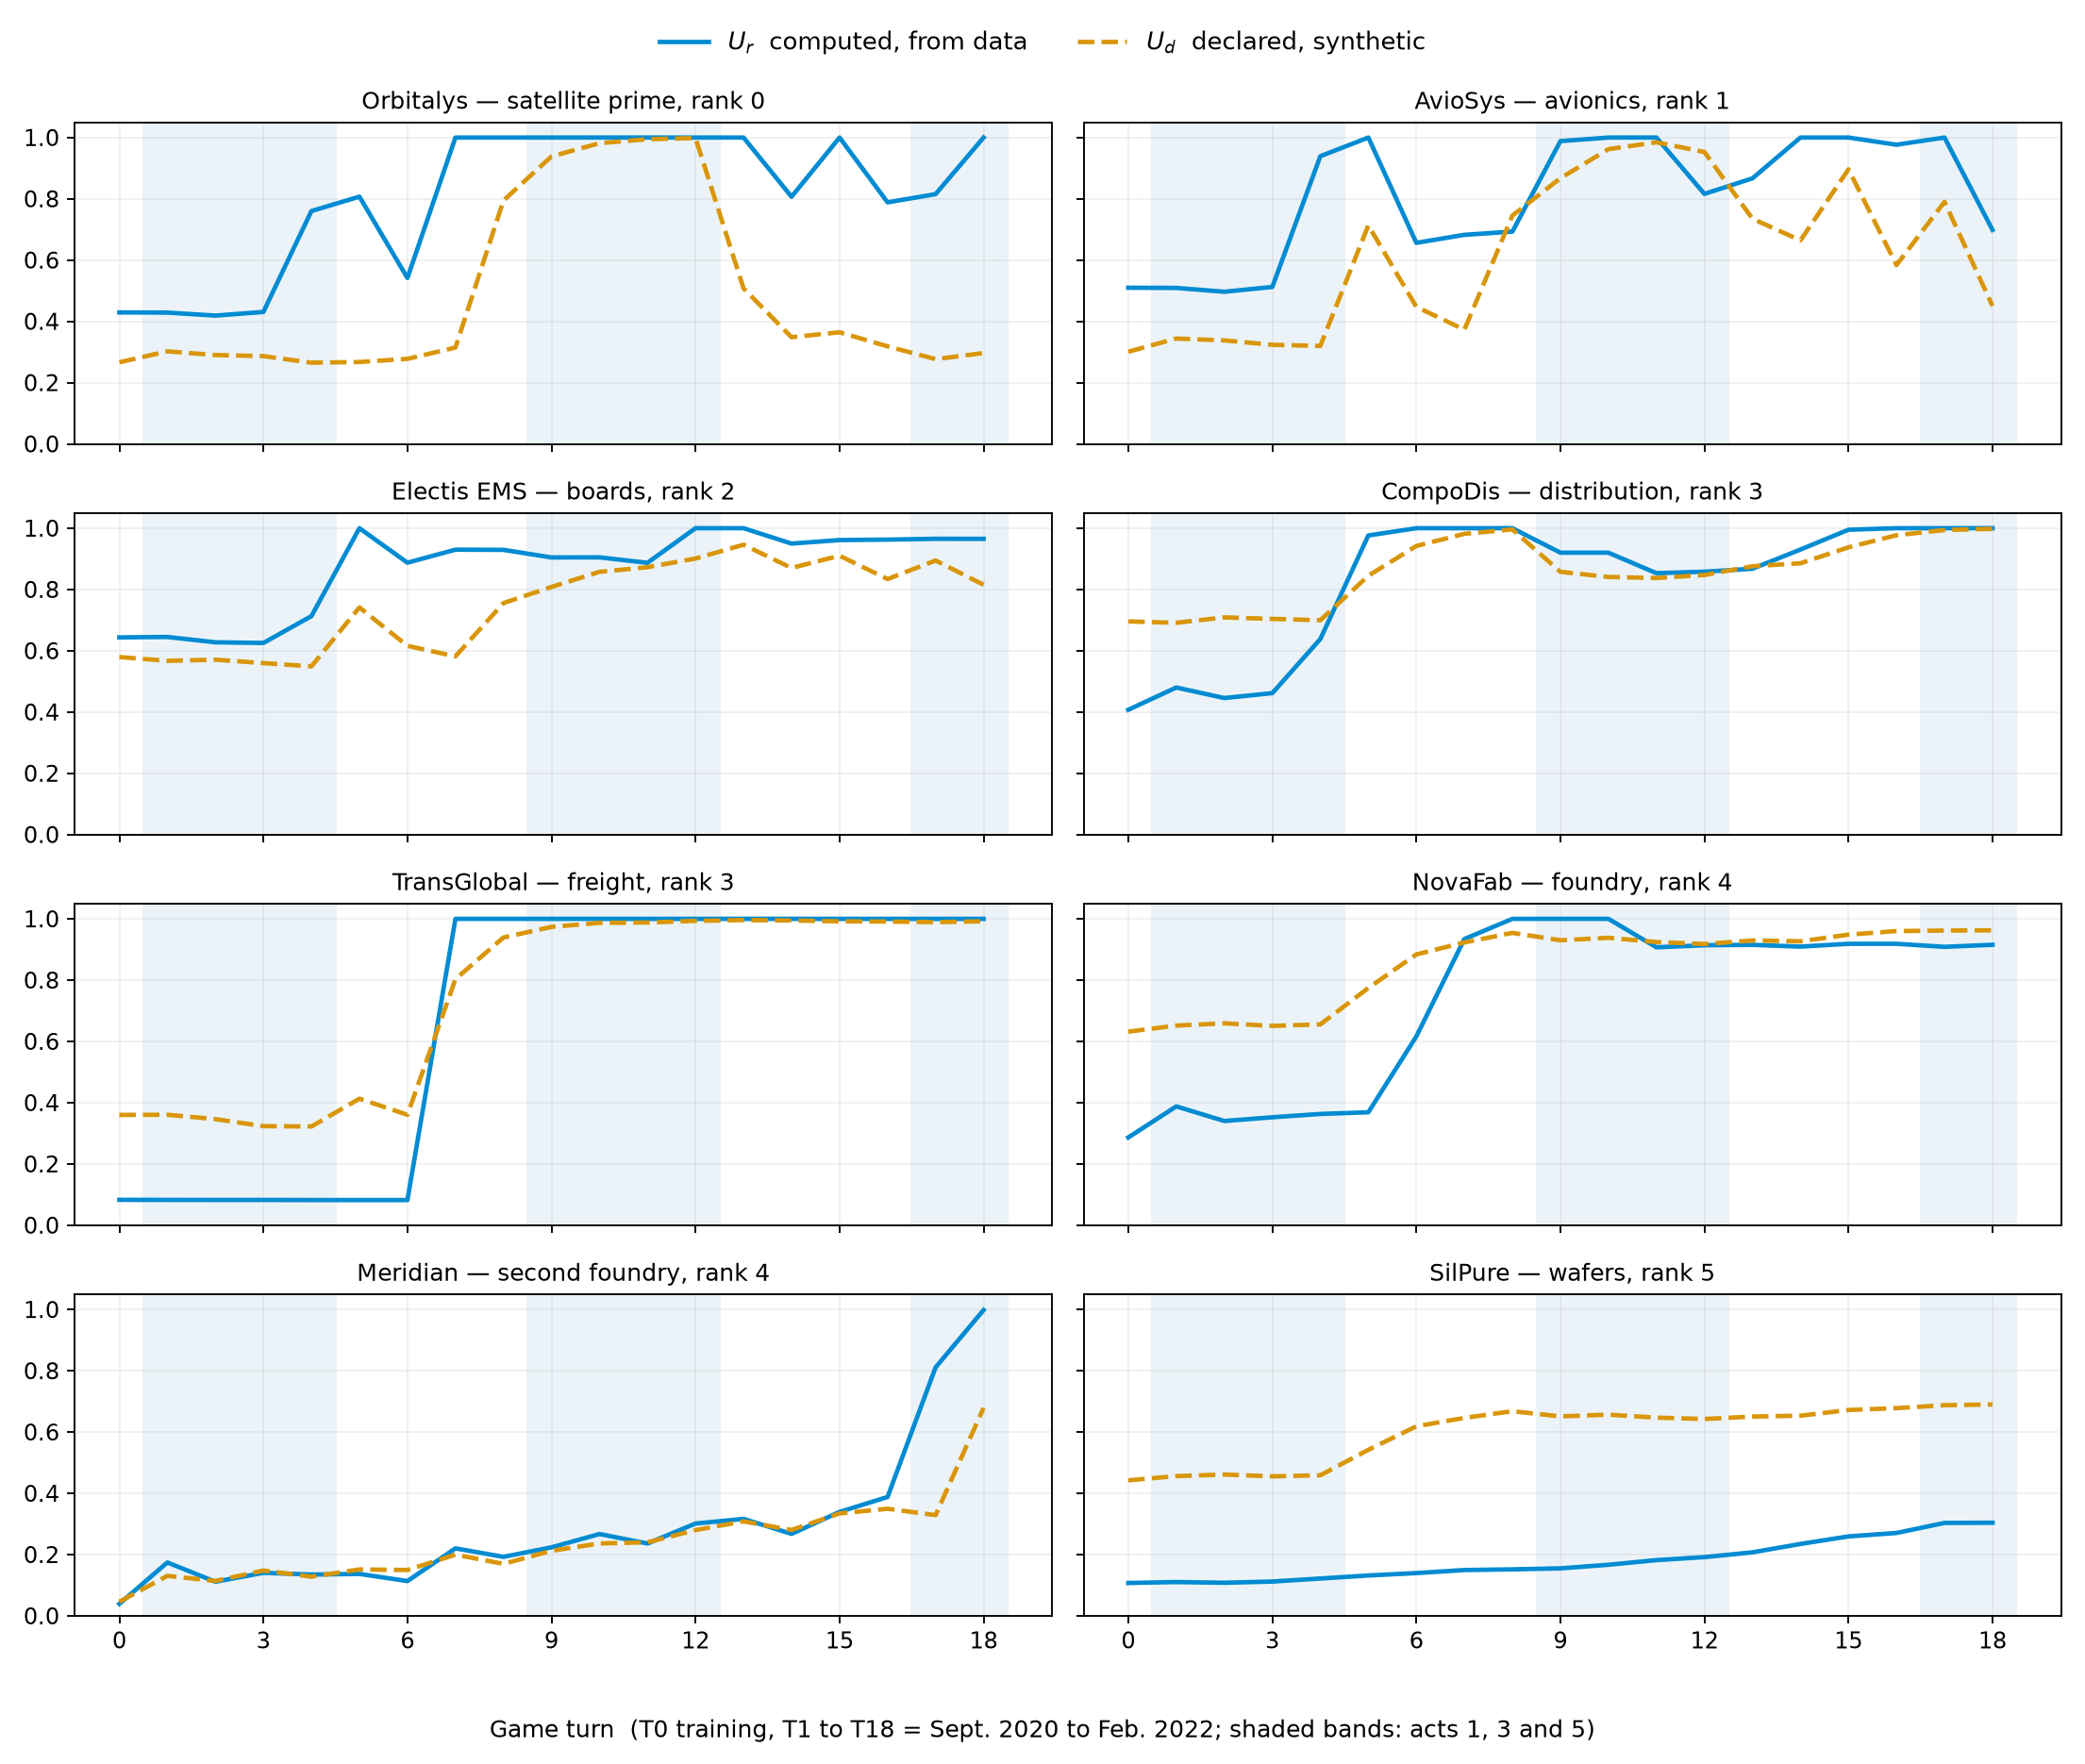
\includegraphics[width=\linewidth]{Images/helios_dryrun_trajectories_en.png}
    \caption{Real against synthetic declared urgency, dry run}
    \label{fig:helios_dryrun_trajectories}
\end{figure}

%% ═══════════════════════════════════════════════════════════════════════════
\subsection{Arm A: Blind Declaration by Eight Isolated Agents}
\label{sec:res_armA}
%% ═══════════════════════════════════════════════════════════════════════════

Arm A replaced the synthetic generator with the eight isolated agents of
Section~\ref{sec:methods_arms}. What matters here is that nothing was simulated around them:
each answered the real AHP questionnaire in character, pairwise comparisons and severity
scores passed through the production consistency-ratio code untouched, and campaign setup,
turn injection and submission went through the same weekly-cycle service a browser-based
participant would reach. Table~\ref{tab:helios_armA} gives the verdicts on the six
pre-registered tests.

\begin{table}[htbp]
\centering
\caption{Arm A verdicts on the six pre-registered hypotheses}
\label{tab:helios_armA}
\small
\begin{tabularx}{\linewidth}{>{\raggedright\arraybackslash}p{3.4cm} >{\raggedright\arraybackslash}p{2.4cm} X}
\toprule
\textbf{Test} & \textbf{Verdict} & \textbf{Measured value} \\
\midrule
H1 latency & Not confirmed & 3 of 8 nodes at lag $\ge 1$ turn (threshold: 5 of 8) \\
H2 early detection & Not confirmed & $H(\text{NovaFab})$ peaks at $0.017$ on turns 6 to 12
(threshold: $0.3$) \\
H3 criticality & Not confirmed & NovaFab top-1 on 7 of 10 informative turns, $70\%$
(threshold: $80\%$; saturated turns excluded per Section~\ref{sec:criticality}) \\
H4 predictive validity & Not confirmed & precision $0.00$, recall $0.00$ at $H \ge 0.5$ \\
H5 contagion & Confirmed & non-affected nodes: $\Delta U_d = +0.079$ on press turns against
$+0.005$ on calm turns \\
H6 hysteresis & Not applicable & real urgency shows no measurable decline over the recovery
turns \\
\bottomrule
\end{tabularx}
\end{table}

Two results stand out. H5 is confirmed: declared urgency at nodes that are not physically
affected rises by $0.079$ on press-event turns against $0.005$ on calm turns, matching the
pre-registered direction and ordering, which is the mere-urgency
effect~\autocite{zhu2018mere} reproduced at network scale. And H4 stays not confirmed for a
specific and informative reason: these agents read their briefing carefully and declared
urgency close to what it described, so $U_d$ tracks $U_r$ too closely to leave the gap that
$H$ is built to catch, more tightly even than the fixed-bias dry run, with
$H(\text{NovaFab})$ peaking at $0.017$ against $0.070$.

Read from the resulting project after the eighteenth turn, the network-average adequacy is
$65.5$, four of the eight nodes carry a hidden-risk reading above $0.1$, one carries a
false-urgency reading above $0.1$, and the worst-scoring node by a wide margin is Orbitalys at
$A = 15.3$ (Table~\ref{tab:armA_snapshot}).

Orbitalys' own explanation page traces the chain from a single scripted event to its score
without manual computation. Its next milestone had slipped past its deadline by turn 18,
which forces $u_{\text{time}}$ to $1$ under the rule of Table~\ref{tab:ur_blocks}; with the
node's real urgency already saturated by this cause alone, the page attributes the whole of
it to the local block and none to the upstream network. The agent playing Orbitalys declared
$U_d = 0.41$, so the hidden risk is $H = 0.59$, penalised through
Equation~\ref{eq:penalty} at $2.25 \times 0.59^{0.88} = 1.42$, giving
$A = 100 \times (e^{-1.42}-e^{-2.25})/(1-e^{-2.25}) = 15.3$, the same number the dashboard
reports. The network-wide PROMETHEE~II ranking places NovaFab and Orbitalys at the top of
the priority list, at $\phi = +0.220$ and $+0.215$, which are the expected bottleneck and
the node its own missed milestone makes most urgent. The same ranking carries a caveat the
tool raises on its own: on this run the time and performance blocks are perfectly
correlated, $\rho = 1.00$, which is exactly the composite-indicator risk flagged in
Section~\ref{sec:lit_mcdm}.

%% ═══════════════════════════════════════════════════════════════════════════
\subsection{What the Adequacy Signal Gets Right: Node-Level Targeting}
\label{sec:res_targeting}
%% ═══════════════════════════════════════════════════════════════════════════

The scoring that follows in Section~\ref{sec:res_armA_scored} asks whether the forecast layer
attaches correct probabilities to node-weeks. That is the right question for a forecast and
the wrong question for the instrument. A coordinator does not act on the proposition that node
$X$ has a $0.14$ chance of an adverse outcome between weeks $t+1$ and $t+4$; they act on a
shortlist of suppliers to look at this week. This subsection scores that, because it is the
decision the adequacy signal was designed to support, and because the answer differs from the
one below.

At each turn the eight nodes are ranked by hidden risk $H = [U_r - U_d]_+$, and the set
flagged at $H > 0.10$ is compared with the set of nodes that go on to miss at least one
milestone at its originally committed deadline, the definition of
Section~\ref{sec:res_target_trap}. Four of the eight nodes are positive under that definition:
the satellite prime, the avionics integrator, the electronics manufacturer and the foundry.
The comparison is at node level and prospective, since the flag at turn $t$ is confronted
with misses occurring later in the campaign. Nothing in it uses the forecast layer.

Table~\ref{tab:targeting} gives the two regimes the campaign separates, and the boundary
between them is the turn on which the scenario's foundry freeze becomes public.

\begin{table}[htbp]
\centering
\caption{Nodes flagged by hidden risk against nodes that later miss a commitment, arm A}
\label{tab:targeting}
\small
\begin{tabularx}{\linewidth}{l >{\centering\arraybackslash}X >{\centering\arraybackslash}X >{\centering\arraybackslash}X >{\centering\arraybackslash}X}
\toprule
\textbf{Regime} & \textbf{Turns} & \textbf{Precision} & \textbf{Recall} &
\textbf{False alarms per turn} \\
\midrule
Before the crisis is public & T0 to T5 & 1.00 & 0.75 & 0 \\
After & T6 to T18 & $\le 0.50$ & 0.25 & 1 to 3 \\
\bottomrule
\end{tabularx}
\end{table}

For six consecutive turns the signal flags exactly three nodes, all three of which later miss
a commitment, with no false alarm on any of the six. The fourth positive node is never
flagged early, so recall stops at three of four. On every one of those turns the worst-scoring
node of the eight is the satellite prime, which misses its turn-8 delivery and delivers at
turn 14: the flag precedes the miss by eight turns, and it is raised while that node's own
manager is declaring an urgency of $0.001$.

That last clause is the construction working as specified rather than a coincidence. The
flag does not come from a pessimistic declaration; it comes from an optimistic declaration
standing against a computed state that is not. A system aggregating indicators alone would
have ranked that node on its indicators. A system collecting declarations alone would have
believed it. Only the difference between the two carries this information, which is the
proposition the thesis set out to test and the one the literature review of
Section~\ref{sec:lit_gaps} found unaddressed.

\subsubsection{Why the Signal Degrades, and What the Sample Supports}

From turn 6 the precision falls to $0.50$ and the recall to $0.25$, for a structural reason.
Once the shortage is public every declarant raises their urgency, $U_d$ converges towards
$U_r$, and a quantity defined as $[U_r - U_d]_+$ shrinks by construction: a perception-gap
measure cannot survive the disappearance of the perception gap. The consequence is a scope
statement rather than a limitation to be repaired. The instrument is an early-warning device
and not a crisis-management one, and its useful window is the interval in which acting is
still cheap. The repair of Section~\ref{sec:res_repair} sharpens the flag without altering
which nodes it selects: at turn 3 the satellite prime scores $26.6$ out of $100$ against
$46.0$ for the next worst node, and after repair the same turn gives $2.2$ against $44.6$,
so the ordering is identical and the separation widens by an order of magnitude.

The standing of the result is bounded and stated plainly. It rests on eight nodes, four of
them positive, over one scripted scenario. A precision of $1.00$ sustained over six turns on
three flagged nodes is an encouraging observation and not an estimated rate: its Wilson
interval runs from $0.44$ to $1.00$, which Section~\ref{sec:res_power} reads against the
interval of the second chain. What would settle it is
more chains rather than a different model.

\subsubsection{The Second Chain, and the Boundary It Draws}
\label{sec:res_second_chain}

A second chain was then built and run: AIRB, an airframer's supply base of fifteen nodes and
thirty arcs over five ranks, with no exogenous shock at any point and three structurally
central suppliers set to degrade endogenously. Its milestone truth is derived from the
indicator trajectory rather than scripted, so a supplier that slows down misses its milestone
because it slowed down. Fifteen declarants, one per node, each seeing only its own monthly
sheet and its own past declarations, played all nineteen turns.

On that chain the adequacy signal does not select the failing nodes at all: across all
nineteen turns, precision at rank three is $0.00$ for both $[U_r - U_d]_+$ and the adequacy
score, against a base rate of $0.20$, while the forecast layer scored on the same runs holds
at $0.56$.

The mechanism is legible in the snapshots and is not a failure of aggregation. The three
degrading suppliers declare the highest urgencies in the chain from turn~0 onwards, before
their indicators have moved: $U_d = 0.94$, $0.88$ and $0.98$ at turn~0, still $0.97$ and
$0.96$ at turn~16 against a computed $U_r$ of $1.00$. A quantity defined as $[U_r - U_d]_+$
is then bounded by $0.03$. Nothing is concealed, so nothing is detected. The nodes that top
the gap ranking at every turn are the downstream assemblers, whose local urgency is
\emph{zero} and whose computed $U_r$ is inherited entirely through the graph from suppliers
they cannot observe.

This is a boundary rather than a refutation, and it is sharper than the scope statement above.
The role cards of those three suppliers described concealers, and the declarants behaved as
such in prose, turn after turn, writing that they would put off calling their customers and
keep overtime in reserve. At the same turns they marked near-maximal severity on the
questionnaire. They minimised in \emph{action} and maximised in \emph{measurement}. The
questionnaire asks what an actor perceives; withholding is something an actor does. A gap
defined between a computed state and a declared perception therefore detects blindness, not
discretion. The synthetic declarants of the semiconductor campaign carried a bias applied to
the number itself, so the gap opened and precision reached $1.00$; a declarant that reasons
does not lower the number.

The claim that survives both chains is therefore narrower: the perception gap is informative
where declarants misjudge their own state, and silent where they judge it correctly and simply
do not escalate. Distinguishing those two failure modes requires an instrument that observes
escalation behaviour and not only declared severity, which the present design does not
provide. Section~\ref{sec:future_work} states it first rather than as a caveat, because it
bears on what the instrument measures and not merely on how well.

%% ═══════════════════════════════════════════════════════════════════════════
\subsection{Arm A Rescored: Discrimination Without Calibration}
\label{sec:res_armA_scored}
%% ═══════════════════════════════════════════════════════════════════════════

The hypothesis verdicts above test the adequacy signal at a single threshold, and a single
operating point cannot distinguish a forecast that orders outcomes badly from one that orders
them well but announces the wrong numbers. This subsection therefore scores all 120
prospective forecasts of arm A, covering turns 4 to 18 across eight nodes, against the
production outcome definition of Section~\ref{sec:methods_scoring}.
Table~\ref{tab:armA_scores} gives the results at each horizon.

\begin{table}[htbp]
\centering
\caption{The arm A forecast layer, scored by horizon}
\label{tab:armA_scores}
\small
\begin{tabularx}{\linewidth}{c >{\centering\arraybackslash}X >{\centering\arraybackslash}X >{\centering\arraybackslash}p{3.0cm} >{\centering\arraybackslash}X >{\centering\arraybackslash}X}
\toprule
\textbf{Horizon} & \textbf{Positives} & \textbf{Base rate} & \textbf{AUC [95\% CI]} &
\textbf{Brier} & \textbf{Brier skill} \\
\midrule
1 week  & 2 & 0.017 & 0.555 [0.470, 0.639] & 0.130 & $-6.93$ \\
2 weeks & 4 & 0.033 & 0.372 [0.258, 0.492] & 0.166 & $-4.14$ \\
3 weeks & 5 & 0.042 & 0.428 [0.315, 0.546] & 0.191 & $-3.77$ \\
4 weeks & 6 & 0.050 & 0.485 [0.389, 0.583] & 0.207 & $-3.36$ \\
\bottomrule
\end{tabularx}
\end{table}

There is no discrimination to speak of. The AUC ranges from $0.372$ to $0.555$ and every
95\% interval contains $0.5$, so on this campaign the forecast does not order node-weeks
better than chance. That statement carries its sample size: the positive class contains
between 2 and 6 observations depending on horizon, far too few to support a confident claim in
either direction, so the campaign provides no evidence of discrimination rather than refuting
it.

The calibration result is much stronger, because it does not depend on the small positive
class in the same way. The Brier skill against climatology is between $-3.36$ and $-6.93$,
meaning the forecast is between four and eight times worse, in mean squared error, than a
trivial forecaster that announces the base rate every time.
Figure~\ref{fig:armA_reliability} bands the four-week forecasts by announced probability and
compares the mean announced value with the observed frequency in each band.

The pattern is unambiguous, each marker's area proportional to the number of forecasts in
its band. Where the model announces a low
probability it is right: 74 forecasts announcing a mean of $0.070$ were followed by an adverse
outcome $8.1\%$ of the time. Where it announces a high probability it is wrong every single
time: twenty-one forecasts announced a mean of $0.948$ and none was followed by the outcome it
predicted. The confusion matrix at the threshold of $0.5$ records 0 true positives, 21 false
positives, 6 false negatives and 93 true negatives.

Hypothesis H4 is stated on a different quantity and should not be read off that matrix: it
tests the hidden risk $H$, not the four-week forecast, at its own threshold of $H \ge 0.5$.
Measured on the campaign database through the production calibration service, that second
matrix reads 0 true positives, 3 false positives, 8 false negatives and 141 true negatives
over 152 node-weeks at four weeks. The two signals fail at the same threshold and for related
reasons, and both return precision and recall of exactly zero, but they are separate
measurements and the H4 verdict rests on the second.

\begin{figure}[htbp]
    \centering
    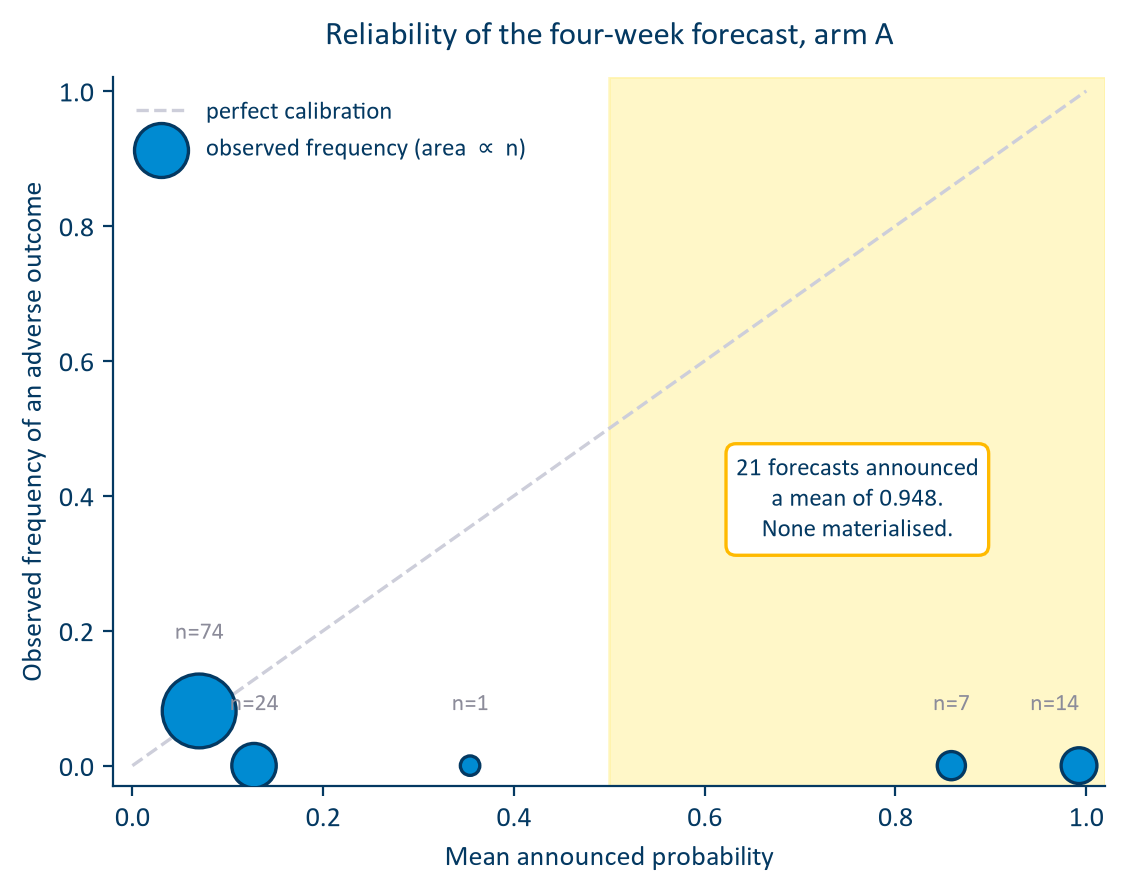
\includegraphics[width=0.86\linewidth]{Images/armA_reliability.png}
    \caption{Reliability of the four-week forecast, arm A}
    \label{fig:armA_reliability}
\end{figure}

The two failures are therefore of different kinds, and this is the dissociation that
Murphy's decomposition anticipates~\autocite{murphy1973vector}: the ordering is
uninformative, and the level is badly wrong at the top of the range while being close to
right at the bottom.

An obvious objection is right-censoring: forecasts made near the end of the campaign have
observation windows extending past the last turn, so if the confident ones were concentrated
there, censoring rather than miscalibration would explain the result. They are not. The
twenty-one confident forecasts are spread over turns 5 to 18 and across seven of the eight
nodes, and repeating the scoring with every forecast whose window runs past the final turn
removed leaves $n = 88$, still 0 true positives against 16 false positives, with the Brier
skill moving from $-3.36$ to $-7.82$: worse rather than better.

\subsubsection{The Mechanism}
\label{sec:res_mechanism}

Figure~\ref{fig:utime_defect} states the defect before the evidence for it.

\begin{figure}[htbp]
\centering
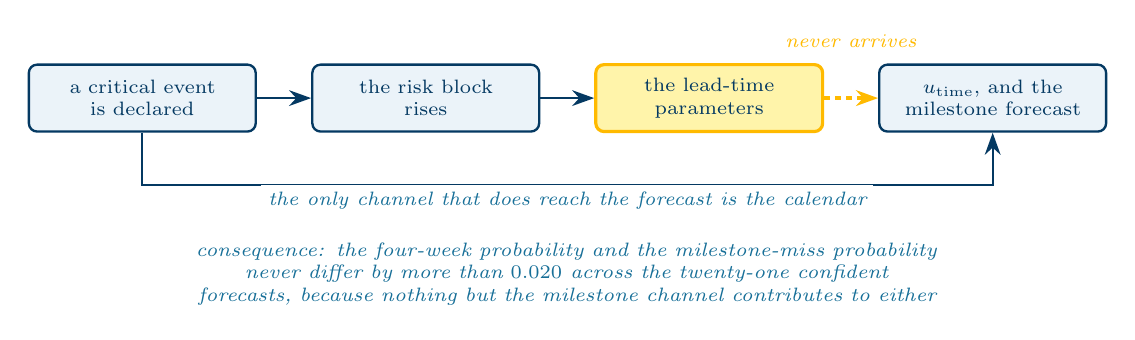
\begin{tikzpicture}[x=1cm, y=1cm, font=\scriptsize,
    st/.style = {bloc, text width=2.6cm, minimum height=0.85cm},
    dead/.style = {blocAlerte, text width=2.6cm, minimum height=0.85cm}]

\node[st] (ev)   at (1.7, 1.2) {a critical event\\is declared};
\node[st] (kpi)  at (5.3, 1.2) {the risk block\\rises};
\node[dead] (lt) at (8.9, 1.2) {the lead-time\\parameters};
\node[st] (ut)   at (12.5, 1.2) {$u_{\text{time}}$, and the\\milestone forecast};

\draw[fleche] (ev) -- (kpi);
\draw[fleche] (kpi) -- (lt);
\draw[flecheCoupee, draw=altenOchreDark, line width=1.3pt] (lt) -- (ut);
\node[etiquette, anchor=south, text=altenOchreDark] at (10.7, 1.75) {never arrives};

\draw[fleche] (ev.south) -- (1.7, 0.1) -- (12.5, 0.1) -- (ut.south);
\node[etiquette, anchor=north, fill=white] at (7.1, 0.1)
     {the only channel that does reach the forecast is the calendar};

\node[etiquette, anchor=north, text width=11cm] at (7.1, -0.55)
     {consequence: the four-week probability and the milestone-miss probability never differ
      by more than $0.020$ across the twenty-one confident forecasts, because nothing but the
      milestone channel contributes to either};

\end{tikzpicture}
\caption[Where the time block stops listening]{The defect located in this section. An event
raises the risk block but never reaches the lead-time parameters that feed
$u_{\text{time}}$, so the milestone forecast is driven by the calendar alone and is blind to
the shocks the scenario injects.}
\label{fig:utime_defect}
\end{figure}

The confident tail has a single source, and the explainability layer of
Section~\ref{sec:explain_export} makes it visible without instrumentation: across all
twenty-one confident forecasts, the four-week probability and the milestone-miss probability
never differ by more than $0.020$. Nothing but the milestone channel contributes to it.

Set against the registry, this is decisive. Of the eighteen milestones in the campaign, ten
completed and eight remained active, none was abandoned, and exactly one was still open past a
deadline that had fallen inside the campaign. The model announced near-certain misses for
AvioSys, CompoDis, \'Electis, NovaFab, TransGlobal and Meridian, and all of them delivered.
That reading is more forgiving than it appears, because the registry stores each milestone's
\emph{current} deadline and a replanning overwrites it, so a milestone re-dated and
subsequently delivered is recorded as completed. Read against the deadline each node
originally committed to, six of the eleven milestones whose original deadline fell inside the
campaign were missed, and five of the twenty-one confident forecasts were followed by a missed
original commitment within four weeks rather than none. The confident tail remains wrong far
more often than right, but the distance between zero of twenty-one and five of twenty-one is
produced entirely by which deadline the truth is read against, which is the subject of
Section~\ref{sec:res_target_trap}.

The same defect is visible directly in the state snapshots, from the opposite side. Reading
the $u_{\text{time}}$ block at turn 6, the turn on which the scenario's one critical event
lands, gives the values of Table~\ref{tab:u_time_turn6}.

Six of the eight nodes read as numerically zero in the middle of a crisis and the seventh
reads as saturated: the block behaves as a step function rather than a risk gradient, either
off or fully on. The cause is structural. The block compares a lead-time distribution against
the time remaining to the next deadline, while the scripted events act on capacity, cost and
failure probability without touching any quantity on the time axis, so a shock never moves
what the milestone probability is computed from. The strongest form of the evidence depends on
no scoring choice at all: across the whole campaign, eight nodes and 41 indicator snapshots
each, the accumulated-delay field the block would need was written a non-zero value exactly
zero times.

This is a defect in the model rather than a property of the scenario, and it is the one
finding of the campaign with a concrete repair. It also invalidates, for this run, the assumption of
Section~\ref{sec:model_blocks} that each block contributes useful information to the
aggregate. One block did not.

%% ═══════════════════════════════════════════════════════════════════════════
\subsection{The Target-Definition Trap}
\label{sec:res_target_trap}
%% ═══════════════════════════════════════════════════════════════════════════

The scores above depend on a choice that is easy to overlook: what counts as an adverse
outcome. Section~\ref{sec:methods_scoring} uses the production definition, requiring a missed
milestone, an abandoned node or an event of gravity critical or defect. Two alternatives are
worth scoring the identical forecasts against: the one an evaluator without access to the
model's own definition would reach for, any event recorded on the node; and one that keeps the
production definition intact but reads a missed milestone against the deadline the node
originally committed to, dropping the forecasts whose window runs past the last campaign turn.
Table~\ref{tab:target_trap} gives the three.

\begin{table}[htbp]
\centering
\caption{The same forecasts under three outcome definitions}
\label{tab:target_trap}
\small
\begin{tabularx}{\linewidth}{X >{\centering\arraybackslash}p{1.1cm}
                                 >{\centering\arraybackslash}p{1.7cm}
                                 >{\centering\arraybackslash}p{1.3cm}
                                 >{\centering\arraybackslash}p{1.9cm}}
\toprule
\textbf{Outcome definition (4-week horizon)} & \textbf{$n$} & \textbf{Base rate} &
\textbf{AUC} & \textbf{Brier skill} \\
\midrule
Production definition: missed milestone, abandonment, or critical event & 120 & 0.050 &
0.485 & $-3.36$ \\[3pt]
Naive definition: any recorded event & 75 & 0.387 & 0.484 & $-0.64$ \\[3pt]
Original-commitment definition: production outcome, deadline as first committed, censored
points excluded & 90 & 0.289 & 0.654 & $-0.55$ \\
\bottomrule
\end{tabularx}
\end{table}

The model is identical, the forecasts are identical, and the horizon is identical. Only the
definition of truth changes. Between the first two rows the measured base rate moves from
$5.0\%$ to $38.7\%$ and the Brier skill improves by a factor of more than five, from $-3.36$
to $-0.64$. An analyst choosing the easier target would report a system that appears five
times better calibrated without a single line of the model having changed.

The third row moves the answer in a different direction and for a defensible reason rather
than a convenient one. Holding the definition of an adverse outcome fixed and only changing
which deadline a milestone is judged against carries the Brier skill from $-3.36$ to $-0.55$
and the AUC from $0.485$, indistinguishable from chance, to $0.654$. The argument for
preferring it is about what a forecast is for rather than about statistics: a replanning is
itself the formal admission of a slip, so a truth in which re-dating erases the miss scores
the forecast against an outcome it was built to warn about before the re-dating happened. It
is the definition used for the re-measurement of Section~\ref{sec:res_repair}, and stating
which of the three any figure refers to is not pedantry: the three disagree by more than any
modelling decision taken in this work.

\begin{figure}[htbp]
    \centering
    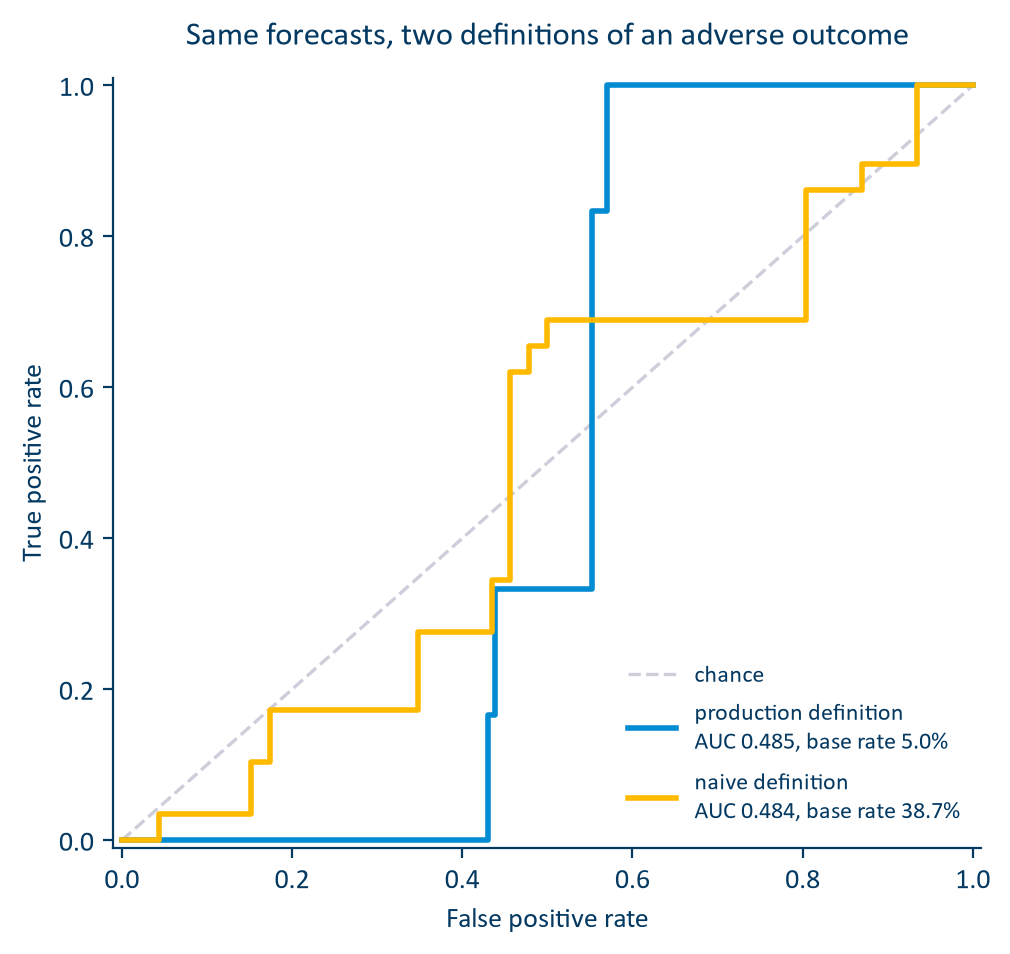
\includegraphics[width=0.86\linewidth]{Images/armA_roc.png}
    \caption{ROC under both outcome definitions}
    \label{fig:armA_roc}
\end{figure}

Discrimination, by contrast, is almost untouched, moving from $0.485$ to $0.484$
(Figure~\ref{fig:armA_roc}). That contrast is itself informative: the ordering of node-weeks is
a property of the forecast, while the apparent quality of the probabilities is substantially a
property of how often the target fires, since a frequent target flatters a forecaster who
announces high probabilities. A calibration figure reported without its outcome definition is
therefore close to meaningless, and the definition belongs in the pre-registration alongside
the thresholds, where the H1 to H6 register does not currently carry it.

%% ═══════════════════════════════════════════════════════════════════════════
\subsection{How Much of This Is Signal}
\label{sec:res_power}
%% ═══════════════════════════════════════════════════════════════════════════

Every score reported so far is a point estimate resting on a positive class of between one
and six observations. The protocol of Section~\ref{sec:methods_scoring} fixed in advance how
such estimates are to be read; this section applies it to the headline claims and states what
survives. Nothing new is measured here. The forecasts, the labels and the scores are the ones
already reported, and only their uncertainty is added.

Table~\ref{tab:auc_tests} tests every arm~A discrimination figure against chance, and
Figure~\ref{fig:auc_forest} draws the same eight rows against the $0.5$ line.

\begin{table}[htbp]
\centering
\caption[Discrimination against chance]{Arm A discrimination against chance, under two
outcome definitions. The interval is the percentile bootstrap; the $p$-value is the exact
conditional test of $\mathrm{AUC}=0.5$}
\label{tab:auc_tests}
\small
\begin{tabularx}{\linewidth}{@{}X c c c c c@{}}
\toprule
\textbf{Outcome definition} & \textbf{$h$} & \textbf{$n$} & \textbf{pos.} &
\textbf{AUC [95\% boot.]} & \textbf{$p$} \\
\midrule
Production            & 1w & 120 & 2 & $0.555$ $[0.470, 0.639]$ & $0.797$ \\
                      & 2w & 120 & 4 & $0.372$ $[0.258, 0.492]$ & $0.388$ \\
                      & 3w & 120 & 5 & $0.428$ $[0.315, 0.546]$ & $0.590$ \\
                      & 4w & 120 & 6 & $0.485$ $[0.389, 0.583]$ & $0.904$ \\
\addlinespace
Naive, any event      & 1w &  75 & 11 & $0.603$ $[0.404, 0.786]$ & $0.279$ \\
                      & 2w &  75 & 19 & $0.601$ $[0.456, 0.741]$ & $0.192$ \\
                      & 3w &  75 & 25 & $0.545$ $[0.409, 0.675]$ & $0.529$ \\
                      & 4w &  75 & 29 & $0.484$ $[0.358, 0.621]$ & $0.823$ \\
\bottomrule
\end{tabularx}
\end{table}

\begin{figure}[htbp]
    \centering
    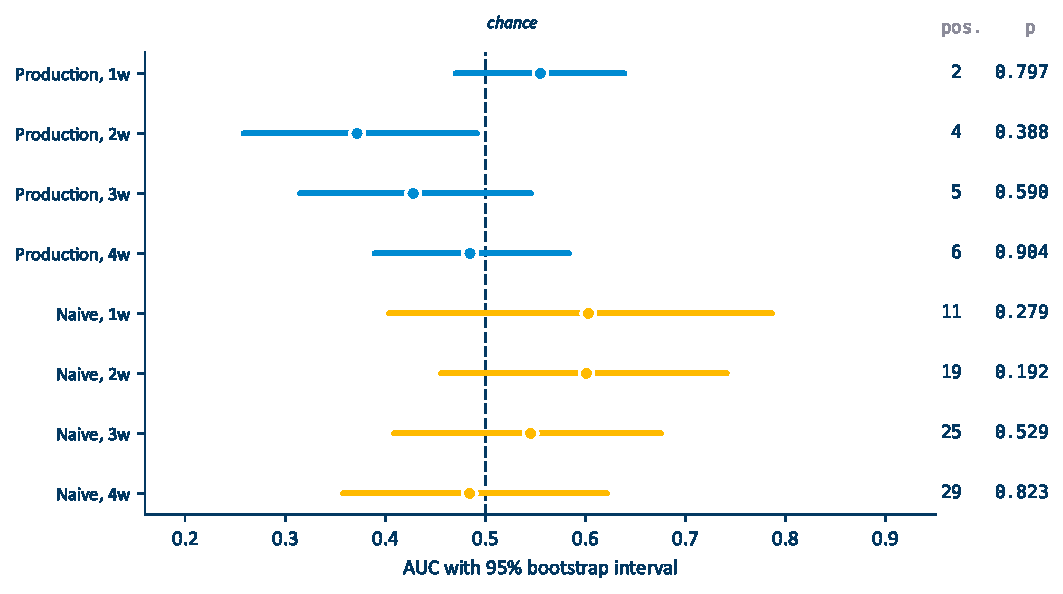
\includegraphics[width=0.94\linewidth]{Images/auc_forest.pdf}
    \caption[Discrimination against chance]{Every arm~A AUC with its bootstrap interval, read
    against the dashed chance line. An interval crossing that line is a result the campaign
    cannot separate from chance. The positive-class size and the exact $p$-value are given at
    the right of each row.}
    \label{fig:auc_forest}
\end{figure}

Not one of the eight is distinguishable from chance. The smallest $p$-value in the table is
$0.192$, and it belongs to the naive definition, the one this thesis argues against using.
The claim of Section~\ref{sec:res_armA_scored} that arm~A discriminates without calibrating
is therefore weaker than the AUC figures alone suggest: what the campaign establishes is that
calibration is bad, which the Brier skills settle at any sample size, and that discrimination
is unproven in either direction rather than demonstrated.

One row deserves separate comment, because it is where the two methods disagree. At two
weeks the bootstrap interval $[0.258, 0.492]$ excludes $0.5$ while the exact test returns
$p = 0.388$. The exact test is the one to follow, and the disagreement has a cause rather
than being a coincidence: with four positives, a bootstrap resample redraws that class with
replacement, so a large share of resamples contains three or fewer distinct positives and the
resulting interval is narrower than its nominal coverage. This is precisely the failure the
protocol anticipated, which is why the interval was recorded as descriptive and the test as
decisive before any of these numbers were seen.

Table~\ref{tab:wilson} does the same for the claims that are counts rather than rankings.

\begin{table}[htbp]
\centering
\caption[Interval estimates for the counted claims]{Wilson $95\%$ score intervals for the
proportions reported on the two chains}
\label{tab:wilson}
\small
\begin{tabularx}{\linewidth}{@{}X c c c@{}}
\toprule
\textbf{Claim} & \textbf{Count} & \textbf{Estimate} & \textbf{Wilson 95\%} \\
\midrule
Chain 1, precision of the adequacy flag & $3/3$ & $1.00$ & $[0.44, 1.00]$ \\
Chain 1, recall over the failing nodes & $3/4$ & $0.75$ & $[0.30, 0.95]$ \\
Chain 1, failure base rate & $4/8$ & $0.50$ & $[0.22, 0.79]$ \\
Chain 2, precision of the adequacy flag & $0/3$ & $0.00$ & $[0.00, 0.56]$ \\
Chain 2, failure base rate & $3/15$ & $0.20$ & $[0.07, 0.45]$ \\
\bottomrule
\end{tabularx}
\end{table}

\begin{figure}[htbp]
    \centering
    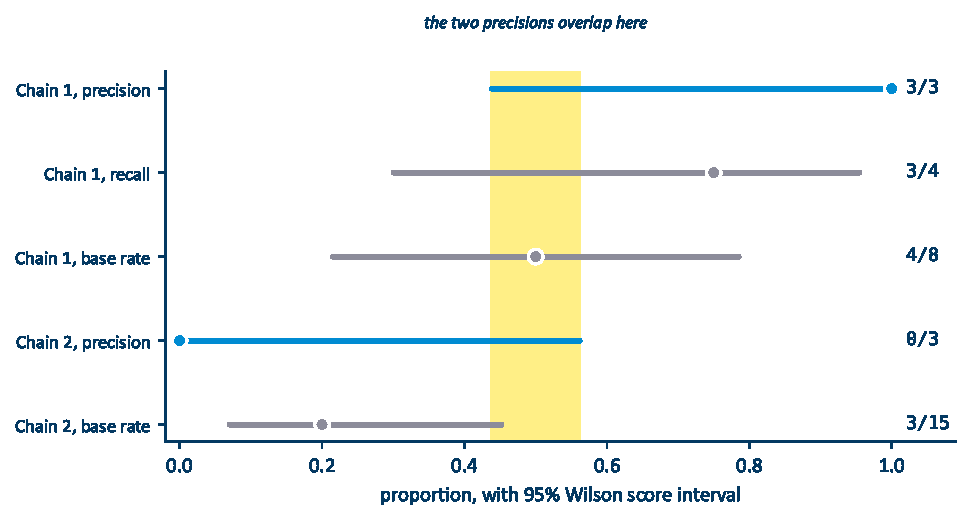
\includegraphics[width=0.94\linewidth]{Images/wilson_intervals.pdf}
    \caption[Interval estimates for the counted claims]{The five proportions with their Wilson
    intervals. The shaded band is the range the two precision intervals share: a precision of
    $1.00$ on three flags and one of $0.00$ on three flags are not, on this evidence,
    distinguishable.}
    \label{fig:wilson_intervals}
\end{figure}

The two precision rows are the ones that matter, and Figure~\ref{fig:wilson_intervals}
shows why: their intervals share the shaded band. The contrast between the two chains, which
Section~\ref{sec:res_second_chain} reads as a boundary, is therefore a difference between two point
estimates and not a demonstrated difference between two populations. That does not make the
boundary wrong, and the mechanism argued for it stands on its own; it means the boundary is
a hypothesis the campaign generated rather than a result the campaign established, and it is
reported as one.

\paragraph{What survives this, and why.}
Three findings do not depend on the size of the positive class, and they are the ones this
thesis rests on.

The first is structural. The defect located in Section~\ref{sec:res_mechanism} is a
property of a code path, not of a sample: the block in question cannot respond to the events
the scenario injects, which is verifiable by reading the propagation of a single event on a
single node and reproducible with one observation. A defect that is present in every run is
not made more or less true by how many runs there are.

The second is a theorem. The collapse of the criticality ranking under saturation is
Proposition~\ref{prop:saturation}, proved from the range and monotonicity of the propagation,
and the campaign merely provides an instance of it in nine turns of nineteen. No inference is
involved.

The third is a within-forecast comparison. The three outcome definitions of
Section~\ref{sec:res_target_trap} score the identical forecasts, so the spread between them
is a fact about the definitions and not an estimate of anything in a population. It needs no
interval because nothing is being generalised.

What does not survive is any statement of a rate. No number in this thesis should be read as
an estimate of how often the instrument would flag correctly in service, and the campaign was
never sized to produce one. Section~\ref{sec:future_work} gives the sample the question would
need.

\paragraph{The same standard applied to the one confirmed hypothesis.}
H5 is the single hypothesis this campaign confirms, and it is reported as a difference
between two means, $\Delta U_d = +0.079$ on press turns against $+0.005$ on calm turns at
nodes that are not physically affected. It carries no interval and no test, and applying the
protocol to the five negative verdicts while exempting the positive one would be the exact
asymmetry the protocol exists to prevent. The comparison is a paired one, the same nodes
observed under two conditions, so a permutation test on the turn labels is available and
costs nothing; it was not run because the per-node-turn declarations behind the two means are
not among the artefacts the derivation script of Section~\ref{sec:methods_repro} currently
exports. That is a reproducibility gap rather than a statistical one,  and it belongs on the list of
Section~\ref{sec:future_work}: until it is closed, H5 should be read as a
confirmed direction of effect and not as a measured effect size.

%% ═══════════════════════════════════════════════════════════════════════════
\subsection{Arm B: What Happens When the Forecast Is Shown}
\label{sec:res_armB}
%% ═══════════════════════════════════════════════════════════════════════════

Arm B replays the identical frozen scenario with the identical eight agents, changing one
thing: from turn 4 onward each agent is shown the predictive analysis of its own node before
declaring. The loop stays open, so the terrain does not change and the forecasts remain
scorable. One property of the design must be established before any interpretation: the
prediction layer is deterministic, so the two arms should carry identical forecasts on the
turns they share, and they do, all 72 shared node-turn forecasts being numerically identical.
Any behavioural difference therefore comes from the act of displaying the forecast, not from a
different forecast being displayed.

The dataset comprises 97 declaration records, reduced to 96 after removing one duplicate
submission at turn 1, each carrying an influence field recording whether the displayed
forecast had no influence, confirmed the agent's assessment, or caused an upward or downward
revision. Figure~\ref{fig:armB_influence} gives the distribution turn by turn.

The first exposure is the result. At turn 4, when the
forecast becomes visible for the first time, all eight agents record an influence and the
direction is entirely one-sided: five revised downward and three had their existing assessment
confirmed. Not one revised upward. The first upward revision anywhere appears at turn 5, and
the scenario's single critical event, the foundry accident, lands at turn 6, two turns after
the moment every declarant was either reassured or confirmed.

\begin{figure}[htbp]
    \centering
    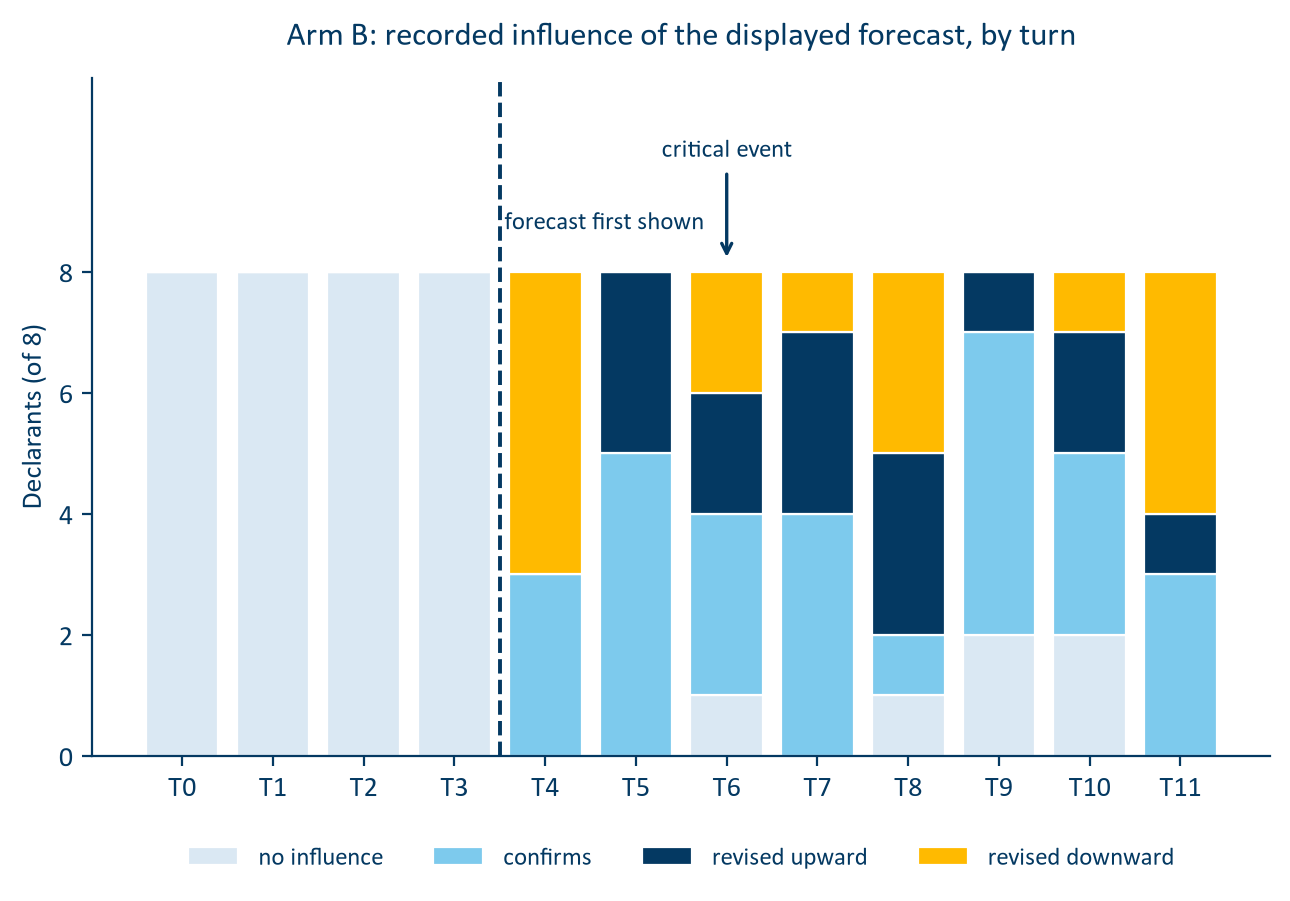
\includegraphics[width=0.86\linewidth]{Images/armB_influence.png}
    \caption{Arm B: influence of the displayed forecast, by turn}
    \label{fig:armB_influence}
\end{figure}

Over the full campaign the distribution is close to balanced, 15 upward against 16 downward,
so what the data shows is a strong first-exposure effect rather than a permanent suppression
of declared urgency. Two factors aggravate it. The forecast displayed at turn 4 is drawn from
the same layer whose confident predictions never materialise and whose $u_{\text{time}}$ block
is blind to the very shock about to arrive. And it is displayed as a numeric probability with
a confidence interval, a format the automation-bias literature identifies as increasing
reliance~\autocite{goddard2012automation,bansal2021whole}. The system was presenting an
unfounded reassurance in the most persuasive available form, immediately before the event it
had failed to anticipate.

One qualification cuts against the strongest reading. The influence field records the effect
on the declared urgency level, not on the decision taken, and the free-text notes show agents
continuing to negotiate allocation, alert the customer and order ahead of schedule at the same
turn. The measured effect is on what was declared rather than on what was done. Since the
declared value is precisely the input the adequacy layer consumes, that is still a
consequential effect on the measurement system.

\subsubsection{The Same Test on the Second Chain}
\label{sec:res_display_second_chain}

The airframer chain of Section~\ref{sec:res_second_chain} was then run a second time with the
forecast displayed, on the same indicator pack and the same derived truth as its control run,
so that the act of display is the only difference between the two. Fifteen declarants,
nineteen turns, 225 forecasts per arm, and 225 declarations made with a forecast on screen.
Figure~\ref{fig:benchmark_predict} carries the three measurements that follow.

Four results follow, and the first is a negative one that simplifies the method. The forecast
scores identically in both arms: a Brier skill of $-1.601$ against $-1.592$ at one week, an AUC
of $0.826$ in both, differences confined to the third decimal, and an unchanged node ranking.
The forecast is computed from indicators the declaration channel does not reach, so the loop is
too weak to close and a treatment arm can be scored exactly as a control arm can. The caution
stated when this campaign was designed, that showing the forecast would destroy the reference,
is refuted by measurement.

The second replicates first contact at five times the scale. On the turn the forecast first
appears, eleven of fifteen declarants report it confirms what they already thought, two revise
downward, and \emph{none} revises upward: the only turn in the campaign without a single upward
revision. One node states the mechanism in its own note, its second lot having sat at zero for
four consecutive turns, which should have raised its time-window urgency further, but the
tool's reading of eleven per cent tempered that concern. The forecast suppressed an escalation
the indicators warranted.

The third qualifies the first two and is the one that generalises. Across all fifteen turns
with a forecast visible, upward revisions outnumber downward ones $26$ to $9$: the one-sided
suppression is a first-exposure effect, and the persistent effect is different and larger. A
declarant follows the number in whichever direction it moves, one node raising its declared
urgency at turn~12 while its own indicators were improving because the tool had risen. The
display does not sedate the operator; it transfers authority from the shop floor to the model,
reassuring when the model is low and the ground is bad, alarming when the model is high and the
ground is good. On a layer whose Brier skill is $-1.59$ at one week, that transfer is the harm,
and it is the composition of two defects documented separately: miscalibration, and display.

The fourth was not sought, and it is the one a designer can act on. The share of declarants reporting that
the forecast changed nothing rises from two at turn~4 to twelve at turn~18, and over the last
four turns seventy-three per cent report no effect. Their reasons are measurable: between
consecutive turns, on the same node and with the terrain unchanged, the median move in the
four-week probability is $0.024$, but fourteen of $139$ moves exceed $0.20$, eight exceed
$0.50$, and the largest is $0.93$. A forecast that falls from thirty per cent to eight in one
turn teaches its reader to stop looking. Disengagement is a rational response to instability
rather than negligence, and it is more costly than the first-contact effect: by the closing
turns, when the layer finally does place a high probability on the supplier that goes on to
miss, no one is reading it.

\begin{figure}[htbp]
\centering
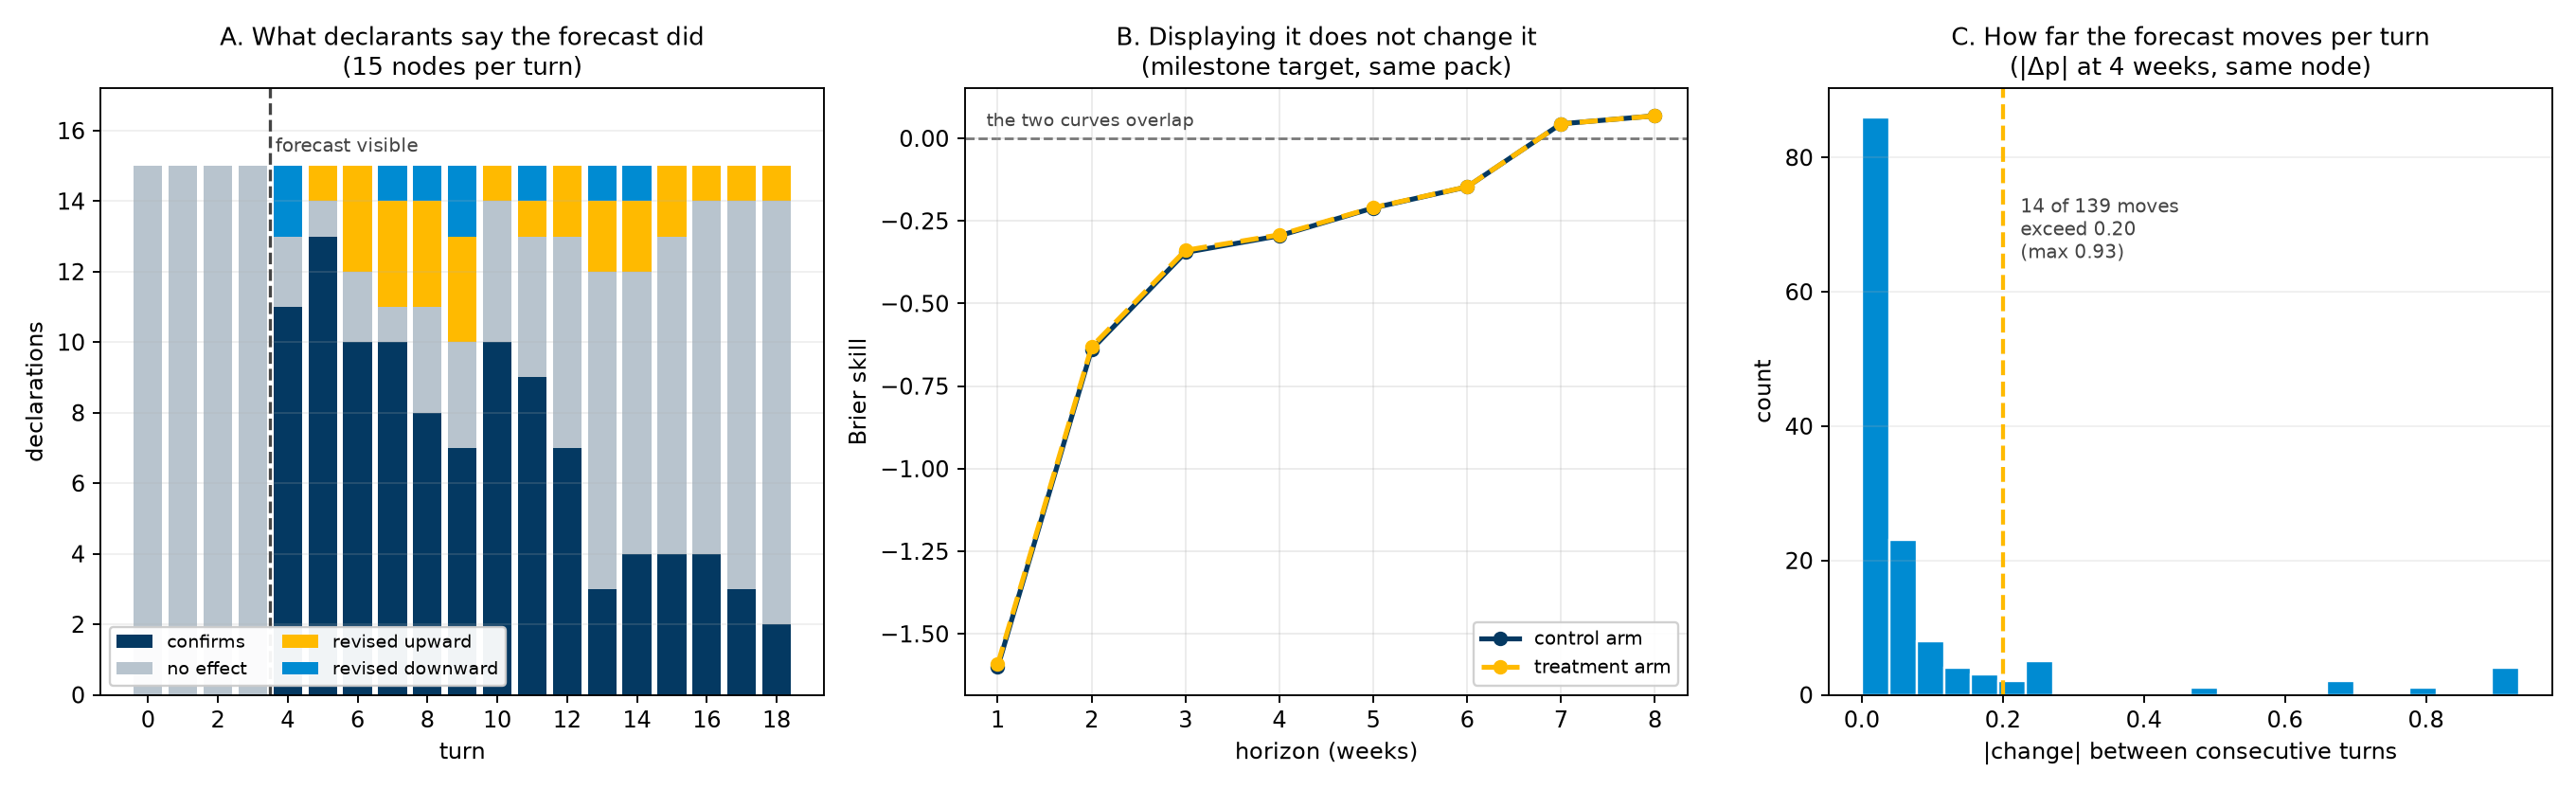
\includegraphics[width=\linewidth]{Images/benchmark_predict.png}
\caption[Displaying the forecast: what changes and what does not]{The second chain, run twice
on one indicator pack. \textbf{A}: what declarants report the forecast did to their judgement,
by turn: first contact at turn~4 produces no upward revision at all, and reported influence
decays as the campaign proceeds. \textbf{B}: the forecast scores identically whether or not it
is displayed; the two curves overlap. \textbf{C}: the turn-to-turn movement of the four-week
probability on an unchanged node, which is what declarants cite when they stop trusting it.}
\label{fig:benchmark_predict}
\end{figure}

\subsubsection{What the Model Being Followed Actually Knows}
\label{sec:res_trivial_baseline}

The preceding result rests on a premise worth testing: that the layer declarants defer to is
doing work a declarant could not do unaided. Two observations put that in doubt. Enriching two
dead indicator blocks on this chain moved computed urgency on $174$ of $285$ node-turns and
left the forecast identical to nine decimal places on $151$ of $154$ comparable points, and
reading the simulation loop explains why. The autoregressive state fitted to local urgency
enters only the client-impact channel; the scored outcome is the disjunction of a milestone
term and an event term, the milestone term depends only on a lead-time draw against the
fraction of the milestone still outstanding, and the event term is empty on a chain carrying no
exogenous shock. Computed urgency never reaches the quantity being scored.

That is a claim about code, so it was tested against a baseline built to be as weak as
possible. For a node whose next unfinished milestone falls due at turn $D$ with fraction $r$ of
its work outstanding and nominal lead time $L$ in turns, the baseline announces
$p(k) = \mathrm{clip}(1 - (D - t - k)/rL,\,0,\,1)$: no simulation, no fitted parameter, no
calibration and none of the six urgency blocks. The service declines to forecast on $71$ of the
$225$ node-turns, where no milestone is in flight, and the baseline is silenced on exactly
those, so both are scored on an identical sample at every horizon.

\begin{figure}[htbp]
\centering
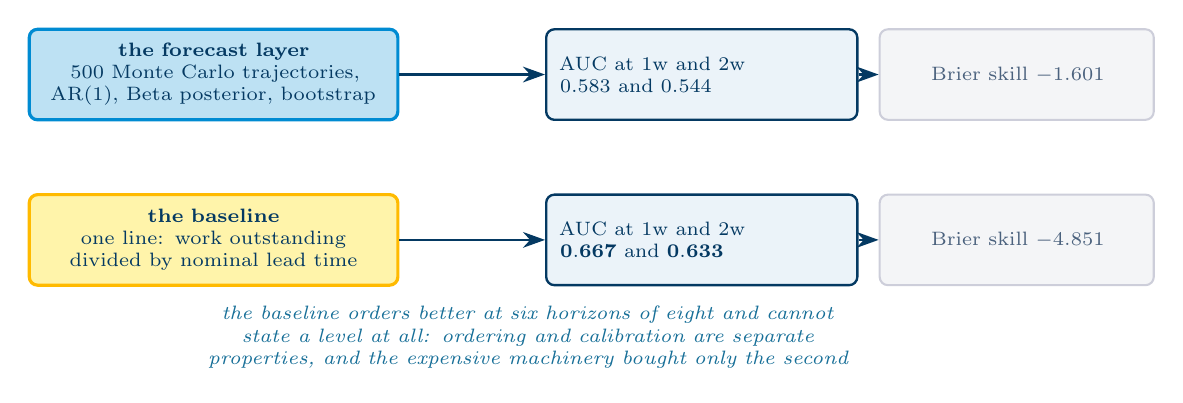
\begin{tikzpicture}[x=1cm, y=1cm, font=\scriptsize,
    bx/.style = {bloc, text width=4.4cm, minimum height=1.15cm, align=left, inner xsep=5pt}]

\node[bx, blocFort] (sim) at (3.0, 1.5)
     {\textbf{the forecast layer}\\500 Monte Carlo trajectories,\\AR(1), Beta posterior,
      bootstrap};
\node[bx, blocAlerte] (base) at (3.0, -0.6)
     {\textbf{the baseline}\\one line: work outstanding\\divided by nominal lead time};

\node[bx, text width=3.6cm] (auc) at (9.2, 1.5)
     {AUC at 1w and 2w\\$0.583$ and $0.544$};
\node[bx, text width=3.6cm] (aucb) at (9.2, -0.6)
     {AUC at 1w and 2w\\$\mathbf{0.667}$ and $\mathbf{0.633}$};

\node[bx, text width=3.2cm, blocPale] (bs) at (13.2, 1.5)
     {Brier skill $-1.601$};
\node[bx, text width=3.2cm, blocPale] (bsb) at (13.2, -0.6)
     {Brier skill $-4.851$};

\draw[fleche] (sim) -- (auc);
\draw[fleche] (base) -- (aucb);
\draw[fleche] (auc) -- (bs);
\draw[fleche] (aucb) -- (bsb);

\node[etiquette, anchor=north, text width=11.5cm] at (7.0, -1.35)
     {the baseline orders better at six horizons of eight and cannot state a level at all:
      ordering and calibration are separate properties, and the expensive machinery bought
      only the second};

\end{tikzpicture}
\caption[A one-line baseline against the simulation]{The comparison that decides whether the
forecast layer earns its complexity. The baseline is silenced on the 225 node-turns where no
milestone is in flight, and on the rest it ranks the misses better while producing no usable
probability.}
\label{fig:baseline}
\end{figure}

The baseline ranks the misses \emph{better} than five hundred Monte-Carlo trajectories at six
horizons of eight. At one week its AUC is $0.908$ against $0.826$ and its PR-AUC $0.396$
against $0.153$; the Monte-Carlo layer regains the advantage only at seven and eight weeks
($0.667$ and $0.633$ against $0.583$ and $0.544$). Since the baseline reads the remaining
fraction from the same progress variable the truth is derived from, it was re-run in a form
that reads nothing at all, remaining work taken as the calendar fraction a perfectly healthy
milestone would show, using only the due date and the nominal lead time. Its AUC and PR-AUC are
identical to three decimal places at every horizon. The discrimination is entirely the ratio of
weeks remaining to weeks required.

What the simulation layer does contribute is visible in the same table and is not
discrimination. Its Brier skill is $-1.601$ at one week against the baseline's $-4.851$: the
baseline produces an ordering and has no means of turning it into a probability, and converting
an ordering into a scale is what the five hundred trajectories are doing. It also holds its
ranking at the long horizons where a calendar ratio collapses, at nearly double the PR-AUC at
seven and eight weeks. The layer is therefore a calibration wrapper around a lead-time ratio,
which is a defensible thing to be, but it is not what the interface presents and not what the
declarants in Section~\ref{sec:res_display_second_chain} believed they were deferring to.

This sharpens rather than softens the display result. Twenty-six upward revisions and nine
downward ones were made in deference to a short-horizon signal that a two-number ratio
reproduces and slightly exceeds: the transfer of authority documented above was not a transfer
to a model that knew more but, at the horizons displayed, to one that knew less. The defect is
nameable and cheap to repair, since the autoregressive state must enter the milestone term and
not only the client-impact term, and the repair would be measurable on these same frozen
forecasts. It was not attempted here, and the sample bounds it: five positives at one week, one
chain, one outcome definition.

%% ═══════════════════════════════════════════════════════════════════════════
\subsection{The Repair, in Brief}
\label{sec:res_repair}

The defect of Section~\ref{sec:res_mechanism} was repaired and the identical frozen forecasts
were rescored against it. Two results belong in the body and the working is in
Appendix~\ref{app:repair}.

The repair changed the recommendation as well as the model. Routing the calibrated events into
the lead time, which is the obvious reading of the diagnosis, does not work: a quantity routed
that way is scaled by the fraction of work remaining, so it attenuates to nothing on exactly
the milestones nearest their deadline. Lost time has to be added to the completion date
instead. The diagnosis was right and the instruction it implied was wrong, which was only
visible because the repair was re-measured rather than assumed to work.

What it bought is bounded. The structural repair lifts both calibration and discrimination at
every horizon, the Brier deficit roughly halving from $-0.553$ to $-0.216$ at four weeks. The
system moves from badly wrong to less wrong, not to useful, and the Brier skill remains
negative throughout. Two further defects surfaced with it: the forecast treated declared
progress as exact, which made the milestone probability binary in $85\%$ of cases, and the
campaign ran at $25.6\%$ indicator coverage with three of six blocks inert.

\subsection{Discussion}
\label{sec:res_discussion}
%% ═══════════════════════════════════════════════════════════════════════════

Six threads run through this discussion and they are not claims of the same kind. Four
survive the sample size because they concern how a measurement is built; two do not,
because they concern how often something happened. Reading them as though they were
equivalent is how a campaign of this size gets over-read.

\paragraph{The circularity problem is the central methodological finding.}
Across the dry run, arm A and arm B, the same difficulty recurs in three different forms.
In the dry run, synthetic declared urgency was anchored on real urgency by construction, so
the gap the system exists to measure could not appear. In arm A, agents read their briefings
carefully and declared close to what the briefing described, so the gap again did not
appear, with $H$ peaking at $0.017$ where the hypothesis required $0.3$. In arm B, showing
the model's own output to the declarant closed the loop explicitly, so the declaration is
no longer independent of the model at all. A system that measures the divergence between a
human judgement and a computed state is only measuring anything when those two quantities
have independent sources. I expected that to be a property of the design. It turned out to
be a property that has to be defended in three separate places, and I missed it in all
three before the data showed me.

\paragraph{Ordering and level are separate problems needing separate fixes.}
The scores of Section~\ref{sec:res_armA_scored} do not support a single verdict on the
forecast layer. On this campaign it neither orders well nor announces well, but the
evidence for those two claims is of very different strength: discrimination rests on between
two and six positive observations and is therefore inconclusive, while the calibration
failure rests on 21 confident forecasts none of which materialised and is not plausibly a
sampling artefact. The remedies differ accordingly. Miscalibration of this shape is
routinely corrected by a post-hoc layer without touching the underlying
model~\autocite{niculescu2005predicting,guo2017calibration}. Poor discrimination is not, and
would require the model to change.

\paragraph{The specific defect is repairable and general, but not in the obvious way.}
The mechanism identified in Section~\ref{sec:res_mechanism} is not a scenario artefact. The
$u_{\text{time}}$ block computes milestone risk from a lead-time distribution against a
deadline, while the event engine writes to capacity, cost and failure probability. No path
connects a shock to any quantity on the time axis, so the block cannot respond to a
disruption, and any deployment of this framework would inherit that gap. The natural repair is to make the calibrated events write a lead-time impact, and
Section~\ref{sec:res_repair} reports that this was implemented, measured and found to be
wrong. The general form of the lesson is that a parameter describing a node's capacity to
recover and a state accumulating what it has already lost carry the same units and are easy to
confuse, and the confusion stays invisible while the database is incomplete.

\paragraph{Communicating ignorance is a design requirement, not a nicety.}
The arm B result reframes what an advisory layer owes its reader. Faced with an exogenous
shock, a weather event, a fire, a geopolitical decision, the model has no basis for
prediction at all. Displaying a low probability in a confident format is then worse than
displaying nothing, because it converts an absence of information into an apparent
reassurance. Two mitigations follow and neither requires new science: make the
horizon salient, so that a low four-week probability cannot be read as a general statement of
safety, and state explicitly which classes of risk the model does not cover. I would now treat
both as acceptance criteria for an advisory layer rather than as refinements to add later.

\paragraph{Threats to validity.}
Four limit what the above can support. The declarants are language models, so the external
validity of any claim about human declaration behaviour is unestablished; this is the
principal threat, and it is why arm B is reported as a measured effect on this population
rather than as a finding about operators. The campaign is a single scenario, so the outcome
base rate, the event mix and the milestone structure are all properties of one script. The
positive class is very small, which bounds every discrimination claim. Finally, arm B is
not blinded, since the agents are told they are being shown a predictive analysis; a design
in which some turns show a deliberately uninformative forecast would separate the effect of
the content from the effect of the display.

\paragraph{Against the pre-registered thresholds.}
Five of the six hypotheses are not confirmed and one, H5 on urgency contagion, is confirmed.
That is a largely negative result against the register, and it is reported as such. The
value of the campaign lies less in those verdicts than in the diagnosis they made possible:
the register asked whether the signal works, and the answer, with its mechanism, is that one
identifiable block prevents it from working and that showing the resulting forecast to the
declarant is actively counterproductive until that block is fixed.

%% ═══════════════════════════════════════════════════════════════════════════


\clearpage
\section{Conclusion}
\label{sec:Conclusion}
%% ═══════════════════════════════════════════════════════════════════════════
\subsection{Contributions}
\label{sec:contributions}
%% ═══════════════════════════════════════════════════════════════════════════

This research set out to determine whether the gap between declared and computed urgency can
be measured reliably enough, inside a working digital twin, to be used as a decision aid
rather than as a descriptive statistic. The evidence gathered answers that in two parts, and
they must not be run together.

As a device for deciding where to look, it works. On the campaign, the nodes the adequacy
signal flags in the six turns before the shortage becomes public are, without a single false
alarm, nodes that go on to miss a delivery commitment, and the worst-scoring of them is
flagged eight turns before its miss while its own manager reports that all is well. As a
device for attaching a calibrated probability to a named week, it does not work yet: the
Brier skill remains negative after a repair that halved it. The first of those is the
decision a coordinator actually takes and the one the architecture was designed around; the
second is a harder problem that the campaign turned from an unknown into a measured distance.

What bounds both statements is the evidence base rather than the design. Eight nodes of which
four are positive, eleven observable milestones and one scripted scenario cannot establish a
rate, however clean the pattern. The contributions below are therefore claimed as a working
instrument with a measured behaviour and a method for interrogating it, not as validated
performance figures.

Five contributions are claimed.

\paragraph{A signal that identifies the right nodes, early, from the gap alone.} Over the six
turns preceding the public onset of the crisis, hidden risk flags three nodes, all three of
which later miss a commitment at its originally committed deadline, with no false alarm on any
turn; three of the four eventual failures are caught, and the earliest and worst is flagged
eight turns ahead. The flag is raised on a node whose declared urgency is $0.001$, which is
the construction working as specified: neither the indicators alone nor the declaration alone
would have selected it, and only their divergence does. The signal weakens once the crisis is
public, which is the expected behaviour of a perception-gap measure rather than a defect, and
it scopes the instrument to early warning. Section~\ref{sec:res_targeting} gives the
measurement and states plainly that four positives cannot establish a rate.

\paragraph{An implemented adequacy architecture.} A multi-block noisy-OR real urgency model,
propagated bidirectionally across a supply chain DAG and confronted with a
consistency-gated, structurally elicited declared urgency through an asymmetric
Prospect-Theory penalty, is specified, implemented and operable. It fills the combination
that Section~\ref{sec:lit_gaps} identifies as absent from the reviewed literature. Its
decomposition is exact rather than approximate, which is what made the diagnosis below
possible from the application rather than by hand.

\paragraph{A diagnosed failure with an identified cause, repaired and re-measured.} The
forecast layer is shown to be badly miscalibrated on the campaign, with a Brier skill between
$-3.4$ and $-6.9$ against a base-rate forecaster and twenty-one confident predictions of
which none materialised under the production outcome definition. That failure is traced to a
single block: the time block computes milestone risk from a lead-time distribution while the
event engine writes only to capacity, cost and failure probability, so no path connects a
shock to the quantity the milestone probability reads. The claim rests on a count rather than
an inference: across the whole campaign the accumulated-delay field was written a non-zero
value exactly zero times, on every node and at every turn. Mid-crisis the block reads as
numerically zero at six of eight nodes.

The repair was then carried out and re-measured on the identical frozen forecasts, and it
changed the recommendation as well as the model. Making the events write a lead-time impact,
the obvious reading of the diagnosis, does not work: a quantity routed into the lead time is
scaled by the fraction of work remaining and therefore attenuates to nothing on the
milestones nearest their deadline. Lost time must be added to the completion date. With that
correction the Brier deficit roughly halves at every horizon, from $-0.553$ to $-0.216$ at
four weeks, and the discrimination rises; the skill nonetheless remains negative, so the
system moves from badly wrong to less wrong rather than to useful. Two further defects were
exposed by the first and are reported with it: the forecast treated declared progress as an
exact value, which made the milestone probability binary in $85\%$ of cases, and the campaign
ran with indicator coverage at $25.6\%$ and three of six urgency blocks inert, which is a
diagnosis about the data rather than the mathematics.

\paragraph{A measured first-exposure effect of showing a forecast to the declarant.} On the
turn the predictive analysis first became visible, all eight declarants either revised their
declared urgency downward or had it confirmed, and none revised upward, two turns before the
scenario's one critical event. Because the two arms are shown to carry numerically identical
forecasts, the effect is attributable to the display rather than to a different prediction.
The finding is reported for a population of language-model agents, and its extension to
human operators is unestablished.

\paragraph{A demonstration that the outcome definition dominates the reported calibration.}
Scoring identical forecasts against a plausible but naive outcome definition instead of the
production one moves the base rate from $5.0\%$ to $38.7\%$ and improves the apparent Brier
skill by a factor of more than five, while leaving discrimination essentially unchanged. A
third definition, which keeps the production notion of an adverse outcome but judges a
milestone against the deadline first committed to rather than the deadline it currently
carries, raises the four-week AUC from $0.485$ to $0.654$ and the skill from $-3.36$ to
$-0.55$. The three disagree by more than any modelling decision taken in this work. The same
trap was then met from the opposite direction: a post-hoc calibration layer fitted against a
target that differed from the product's improved calibration while degrading ranking, and was
deliberately not connected. A calibration figure reported without its outcome definition
carries little information, and a calibration layer fitted without checking its target can
degrade a system that works.

A sixth result, reported as an opening rather than a contribution, establishes that
individual loading docks are not observable from directly overhead because of canopy
occlusion rather than insufficient resolution, and that the reframed problem of delimiting an
equipped facade is both learnable and sufficient for capacity estimation.

%% ═══════════════════════════════════════════════════════════════════════════
\subsection{Status of the Research Hypotheses}
\label{sec:hypothesis_status}
%% ═══════════════════════════════════════════════════════════════════════════

Table~\ref{tab:hypothesis_status} gives the status of each pre-registered hypothesis across
the three runs. It is the single authoritative statement of those verdicts in this thesis.

\begin{table}[htbp]
\centering
\caption{Status of the six hypotheses across the executed runs}
\label{tab:hypothesis_status}
\small
\begin{tabularx}{\linewidth}{>{\raggedright\arraybackslash}p{2.5cm} >{\raggedright\arraybackslash}p{2.1cm} >{\raggedright\arraybackslash}p{2.1cm} X}
\toprule
\textbf{Hypothesis} & \textbf{Dry run} & \textbf{Arm A} & \textbf{Reading} \\
\midrule
H1 latency & Not confirmed & Not confirmed & 1 of 8 nodes on the dry run, 3 of 8 in arm A
against a threshold of 5. The direction is right and the level is short. \\
\midrule
H2 early detection & Not confirmed & Not confirmed & $H$ peaks at $0.070$ then $0.017$
against a threshold of $0.3$. The declared signal tracks the computed one too closely for a
gap to open. \\
\midrule
H3 criticality & Not confirmed & Not confirmed & Top-1 on 7 of 10 informative turns, $70\%$
against a threshold of $80\%$. Identical across runs, since the test does not depend on
$U_d$. Nine turns were excluded as saturated; Section~\ref{sec:res_repair} reports what a
log-survival sort key recovers from them, as an exploratory re-measurement rather than a
revised verdict. \\
\midrule
H4 predictive validity & Not confirmed & Not confirmed & Precision and recall both $0.00$ at
the threshold. Section~\ref{sec:res_mechanism} attributes this to the time block rather than
to the adequacy formulation. \\
\midrule
H5 contagion & Not confirmed & \textbf{Confirmed} & $\Delta U_d = +0.079$ on press turns
against $+0.005$ on calm turns. The mere-urgency effect reproduced at network scale. \\
\midrule
H6 hysteresis & Not applicable & Not applicable & Real urgency shows no measurable decline
over the recovery turns, so the comparison is not meaningful on this scenario. \\
\bottomrule
\end{tabularx}
\end{table}

One hypothesis of six is confirmed. Three qualifications belong with that count. H4 fails for
an identified mechanical reason rather than because the adequacy concept is unsound. That
mechanism has since been repaired (Section~\ref{sec:res_repair}), but H4 has \emph{not} been
re-decided here: the verdict is a precision and recall measured on the arm A declarations at
a pre-registered threshold, and re-running it on a model that has changed would not answer
the question the register asked. It should be re-decided on the human campaign, against the
repaired model, with the outcome definition written into the register. H6 was never testable
on this scenario, because the script does not de-escalate far enough for a decay rate to be
compared, which is a design fault in the scenario rather than a result.

%% ═══════════════════════════════════════════════════════════════════════════
\subsection{Limitations}
\label{sec:limitations}
%% ═══════════════════════════════════════════════════════════════════════════

Table~\ref{tab:limitations} lists the limitations judged material enough to state directly,
with their operational implication.

\begin{table}[htbp]
\centering
\caption{Documented limitations and their implications}
\label{tab:limitations}
\small
\begin{tabularx}{\linewidth}{>{\raggedright\arraybackslash}p{4.4cm} X}
\toprule
\textbf{Limitation} & \textbf{Implication} \\
\midrule
The time block was blind to shocks, and the repair does not make it good & Measured, not
suspected: on the campaign the calibrated events wrote nothing on the time axis, so milestone
risk could not respond to a disruption and read as numerically zero mid-crisis at six of
eight nodes. This is the cause of the H4 failure. The path has since been built and measured
(Section~\ref{sec:res_repair}); the Brier deficit halves and remains negative, and the
milestone probability is still binary in $71.7\%$ of cases. \\[3pt]
\midrule
The campaign ran on a quarter of its indicators & Coverage on the campaign database was
$25.6\%$, with 24 of 42 indicators empty on every node and only three of the six urgency
blocks contributing. A node with no lead time received a risk floor of zero through a
documented fallback, so an absence of data presented itself as a reassuring prediction. Any
calibration performed before this was found would have been fitted to that absence. \\[3pt]
\midrule
One predictive indicator class is missing rather than empty & The model reads current flow
but not the forward booking horizon, that is, how far ahead a node's capacity is already
sold. In the real shortage that signal preceded the degradation of every flow indicator by
months. The gap is general to any capacity-constrained link, not specific to
semiconductors. \\[3pt]
\midrule
Validation rests on agent declarants & The campaign was executed with eight isolated
language-model agents, not human consultants. Every statement about declaration behaviour is
a statement about that population. The human campaign, for which the protocol is frozen, has
not been run. \\[3pt]
\midrule
A single scenario, with a very small positive class & All results come from one
nineteen-turn scenario in which between two and six node-weeks are positive depending on
horizon. Discrimination claims are correspondingly weak in both directions. \\[3pt]
\midrule
No probabilistic guarantee & The framework produces probabilities, scores and confidence
intervals, not certainties, and the campaign showed those probabilities to be poorly
calibrated at the top of their range. \\[3pt]
\midrule
Score freshness follows input cadence & Without an ERP connector, a node's score is never
more current than its last submitted weekly review. Manual entry is an accepted trade-off,
not an oversight, and Section~\ref{sec:res_volume} reports one route out of it for a single
block. \\[3pt]
\midrule
Blocks are assumed independent & The noisy-OR aggregation requires it, and the campaign
produced a counter-example: two blocks were perfectly correlated on the arm A run, which the
tool flagged on its own. \\[3pt]
\midrule
AHP is limited to four criteria & Saaty's method degrades past roughly seven pairwise
compared criteria, which is why declared urgency stays on four while the larger set of KPI
blocks is weighted through Fuzzy BWM instead. \\[3pt]
\midrule
Event calibration priors are defensible, not measured & The Beta-Bernoulli prior weight and
the EMA reactivity coefficients follow standard conjugate Bayesian revision but are not
empirically fitted. \\[3pt]
\midrule
Event reversibility is conditional & Reverting a declared event is guaranteed correct only if
no other write has touched the same KPI in the meantime; otherwise the system raises an
explicit conflict rather than silently rebasing later writes. \\[3pt]
\midrule
Double counting is possible & An operator can both declare a calibrated event and manually
correct the same KPI in the same week. The interface warns but does not forbid it, since the
human operator remains the final authority. \\[3pt]
\midrule
The satellite capacity model is not connected & It reaches one block of six, covers
metropolitan France only, produces a structural capacity rather than a live occupancy, and
its trained segmentation model is not yet wired into the production capacity path. \\[3pt]
\midrule
The fill factor is not reproducible from the retained data & The production constant of
$0.80$ comes from a 122-site calibration whose detailed output was not kept. Recomputing over
the 68 sites still on disk gives a median of $0.97$. Volumetric outputs therefore carry an
unquantified bias of order twenty per cent until the corpus is recollected. Dock capacity,
which depends on the pitch constant instead, is unaffected. \\
\bottomrule
\end{tabularx}
\end{table}

%% ═══════════════════════════════════════════════════════════════════════════
\subsection{Future Work}
\label{sec:future_work}
%% ═══════════════════════════════════════════════════════════════════════════

The work divides into what must happen before the framework can be evaluated fairly, and
what becomes worth doing afterwards. Two items dominate both lists and are stated first
because every other entry is bounded by them.

\paragraph{Separate misperception from discretion; the present instrument cannot.} The second
chain (Section~\ref{sec:res_second_chain}) established that $[U_r - U_d]_+$ selects failing
nodes when declarants misjudge their own state and selects nothing when they judge it
correctly and choose not to escalate. Both are concealment operationally, and only the first
is visible to a questionnaire, because a questionnaire records what an actor perceives while
withholding is something an actor does. This is the sharpest open question the work raises,
and it is a question about \emph{what} is measured rather than how well. Two routes are
available and neither requires new theory: instrument the escalation channel itself, so that
the interval between a declarant recognising a problem and communicating it downstream becomes
observable alongside the declared severity; or read the free-text note the system already
collects at every turn, in which the declarants of the second chain stated their intention to
delay contacting their customers while marking near-maximal severity in the same submission.
The second route costs nothing in data collection and would be the natural first test, with
the caveat that a measure taken on generated text must be validated against human declarants
before it can carry weight.

\paragraph{Widen the evidence base; it remains the binding constraint.} The quantitative
claims of this thesis rest on two chains: eight nodes with four positives and eleven
observable milestones on one scripted scenario, and fifteen nodes with three positives and
twenty-two observable milestones on a second, unscripted one. That is why a precision of
$1.00$ over six turns is reported as an observation rather than a rate, why the confidence
interval on the four-week AUC spans $0.21$ to $0.87$, and why no movement in discrimination
between model versions can be attributed. The second chain was worth its cost --- it bounded a
central claim, which one chain could not have done --- and it also shows the limit of the
approach: two scenarios authored by the same hand cannot separate a property of supply chains
from a property of the author. None of this is repaired by a better model. It is repaired by
running the same instrument on more chains, longer horizons and more milestones, and three
routes are open without new science: replaying further documented disruptions on the same
harness, which costs only scenario authoring; instrumenting a live chain through the weekly
review, which the system already supports; and generating scale synthetically for the
calibration layer while keeping the real campaigns as the evaluation set. A campaign an order
of magnitude larger in positives would let the node-level result be stated as a rate with an
interval, and would let the calibration layer be trained on the product's own target, which is
the single step currently blocking a positive skill.

\paragraph{The time block is repaired, and doing it corrected the instruction.} This thesis
first recommended making the calibrated events write a lead-time impact. That was
implemented, measured and found wrong (Section~\ref{sec:res_repair}): lost time must be added
to the completion date, not multiplied into it, or the shock vanishes on exactly the
milestones a warning would serve. The generalisable form is that a parameter describing a
node's capacity to recover and a state accumulating what it has already lost share their
units and are easy to confuse, and the confusion stays invisible while the database is
incomplete. What remains on this axis is smoothing the milestone alarm, which today moves
from $0.05$ to $1.00$ in a single turn and is correct but unusable as advance warning.

\paragraph{Fill the indicators before calibrating anything else.} The campaign that produced
the negative result ran at $25.6\%$ coverage with half the urgency blocks inert. Completing
them from public figures of the shortage raised coverage to $49.1\%$, activated all six
blocks, and exposed one model bug that had been undetectable while the database was empty. No
amount of calibration compensates for a missing input, and this step is the only one on the
list that is general by construction: it tunes no constant to this scenario.

\paragraph{Rebuild the calibration layer's training label on the product's target.} The
reliability profile of Section~\ref{sec:res_armA_scored} is the shape that post-hoc
calibration addresses~\autocite{niculescu2005predicting,guo2017calibration}, and the
correction is a thin layer rather than a model change. Such a layer was trained off-scenario
on a synthetic factory, which respects the constraint that it must not be fitted to the
evaluation data, and measured: it improves the Brier skill by $30.8\%$ on its own training
distribution, and on the campaign it improves calibration while dropping the four-week AUC
from $0.721$ to $0.580$. Its label is an event at exactly $t+1$; the product displays a
missed milestone or a critical event over $(t, t+4]$. It is therefore not connected.
Connecting it requires the synthetic factory's snapshots to record milestone truth so that
the training label can be aligned with what the product shows, which is a concrete blocked
step rather than an open question.

\paragraph{Make the forecast state its own ignorance.} Given the arm B result, an advisory layer
that cannot anticipate exogenous shocks should not present a low probability in a confident
numeric format. Two changes follow directly: make the horizon salient in the display, so a
low four-week figure cannot be read as general safety, and state explicitly which risk
classes the model does not cover.

\paragraph{Re-run the comparison with the display controlled.} Arm B is not blinded. A design in
which some turns display a deliberately uninformative forecast would separate the effect of
the content from the effect of the display, and would establish whether the first-exposure
effect is a response to the numbers or to being given a number at all.

\paragraph{Run the human campaign.} The frozen protocol, the hashed data pack and the
operating scripts are ready. Only the human campaign can decide the hypotheses as they were
written, and it should now be run against the repaired model rather than against the
known-defective one, which would have wasted the participants.

Arm C, the closed loop in which declarants act on the terrain, has been executed in its
agent version on the repaired system (Section~\ref{sec:res_repair}), and its result sets the
expectation for the human run rather than replacing it. Judged as it must be, by final state
rather than by prediction accuracy, it met five milestones of eleven on their original
commitment against five of eleven for arm A: the loop changed which milestone was met, not
how many, saving one and replanning one that would have held. With eleven milestones that is
a fact of one campaign and not a result, and it is the quantity the human run should be
powered to measure.

\paragraph{Put the outcome definition in the pre-registration.} Section~\ref{sec:res_target_trap}
shows the outcome definition moving the reported skill by a factor of five. It belongs
alongside the numeric thresholds in the H1 to H6 register, where it currently is not.

\paragraph{Connect the observed capacity channel.} Three steps stand between the satellite work
and a usable input: wire the trained segmentation model into the production capacity path in
place of the trailer-span method, re-measure the no-signature rate on an unbiased draw, and
recollect the regulatory corpus cleanly to re-derive the fill factor. Beyond those, the
surface model from LiDAR is the most promising unexplored route, because the canopy step is
several metres lower than the main roof and would give both the canopy extent and the true
roof edge, correcting the 0 to 14.4~m overhang that currently displaces the apron boundary.
One governance question must also be settled rather than deferred: the detection library is
distributed under a copyleft licence, which is immaterial for internal use but becomes
determinative the moment the capability is distributed or exposed over a network.

\paragraph{Broaden the elicitation and couple the platforms.} Two directions identified but
deliberately descoped remain open: replacing single-operator AHP elicitation with a
multi-expert protocol aggregating several judgments per node, and coupling SupplyScore with
the DISCO platform it currently runs alongside rather than inside. Neither is a design
commitment, and both depend on what a repaired system shows.

%% ═══════════════════════════════════════════════════════════════════════════
\subsection{Personal Conclusion}
\label{sec:personal}
%% ═══════════════════════════════════════════════════════════════════════════

\subsubsection{Technical Skills Developed}

The project drew on four distinct areas, and the difficulty of the subject lay mostly in
making them work together rather than in any one of them.

\begin{itemize}
    \item \textbf{Multi-criteria decision analysis}: pairwise elicitation through AHP and
    Fuzzy BWM, consistency validation, and outranking aggregation through PROMETHEE~II.
    \item \textbf{Probabilistic modelling}: noisy-OR aggregation, Monte Carlo simulation,
    conjugate Bayesian revision in a sparse-data regime, and, added during the campaign
    analysis, probabilistic forecast verification through proper scoring rules and
    reliability decomposition.
    \item \textbf{Graph algorithms}: propagation over a multi-rank directed acyclic graph,
    topological ordering, shock simulation and network criticality.
    \item \textbf{Software engineering}: architecture of a multi-tenant Python system,
    hardened SQLite persistence with write-ahead logging, backup and migrations, a Dash web
    interface, and a milestone-based quality process with blocking test coverage and
    automated end-to-end tests.
\end{itemize}

The satellite work added a fifth: geospatial data engineering against public web services,
dataset construction and annotation, and the training and evaluation of a segmentation model
under a strict CPU budget.

\subsubsection{What I Learned}

The hardest problem was not mathematical. It was recognising, three separate times, that the
system was measuring itself. The dry run anchored declared urgency on real urgency by
construction; the agents in arm A read their briefings so carefully that their declaration
reproduced the computed state; and arm B closed the loop deliberately by showing the model's
own output to the declarant. Each time the symptom looked like a modelling problem and each
time the cause was circularity in the measurement. I would now design the independence of
the two signals first, before designing either of them.

The second lesson concerns what counts as a result. For a long stretch of the project I
treated a negative outcome as a failure to be fixed before reporting. The most useful
findings in this thesis are negative: the forecast layer is badly calibrated, the confident
tail is entirely false, one block is structurally blind, and showing that forecast to a
declarant is counterproductive. None of those would have been found by a project optimising
for a positive result, and each of them is actionable in a way that a marginal improvement
would not have been. The related discipline, which the annotation episode of
Section~\ref{sec:res_volume} taught bluntly, is that a confident self-report is not evidence,
whether it comes from an automated process or from oneself, and that the cheap verification
step should always come before the expensive one.

With hindsight I would change two things. I would have scored the forecast layer against
recorded outcomes far earlier, since doing so took a few hundred lines and revealed the time
block defect immediately, where months of implementation had not. And I would have written
the outcome definition into the pre-registration alongside the thresholds, having since
measured how much it moves the answer.

The skill that progressed most was not a technical one. It was the willingness to state a
result that does not flatter the work, in enough detail that someone else can act on it. The
subject of this thesis is, after all, the gap between what people declare and what is
actually true, and it would be a poor outcome to have measured that gap in a supply chain
while reproducing it in the reporting.

Professionally, the project confirmed a direction. I want to work where a model meets the
person who has to act on it, because that boundary is where the interesting failures live:
not in the mathematics, which can be checked, but in what a number does to the judgment of
the person reading it.


\clearpage
\printbibliography[heading=bibintoc, title={References}]

\clearpage
\appendix
\section{Ethics Documentation}
\label{app:ethics}

The study as executed involves no human participants. The eight declarants of the H\'ELIOS
campaign are language-model agents, and no personal data was collected, processed or stored
at any stage. On that basis the project was submitted to the Cranfield University Research
Ethics System as a low-risk study, and the approval documentation is filed with this thesis.

Two features of the protocol would require participant consent if the campaign were rerun
with the eight human consultants for whom it was originally designed, and both are recorded
here so that the requirement is not lost.

\paragraph{Incomplete disclosure through the cover story.} Participants are told they are
playing a fictional satellite programme. They are not told that the scenario replays the
documented 2020 to 2022 semiconductor shortage, because a participant who recognised the
historical chronology could anticipate events rather than react to them, which would destroy
the latency measurement that hypothesis H1 depends on. The debrief reveals the real scenario
and asks each participant at which turn they recognised it, which converts the principal
threat to the measurement into a recorded quantity.

\paragraph{Deliberate misinformation through the placebo sheets.} Two participants receive a
false de-escalation notice, one at turn 9 and one at turn 15. These sheets control for
suggestibility: a declared urgency that follows the placebo is reflecting the sheet rather
than a reading of the situation. Participants are not told in advance which sheets are
genuine.

Both are standard incomplete-disclosure designs in behavioural operations research, and both
are resolved by the full debrief. Were the human campaign to run, the following would need to
be in place before the first turn: written informed consent covering the use of incomplete
disclosure; the unconditional right to withdraw at any point, with the participant's data
removed on request; the debrief protocol, delivered to every participant regardless of
whether they completed the campaign; and confirmation that no performance data is passed to
line management, since the participants would be colleagues and the campaign records their
judgment quality week by week.

\paragraph{Data ethics for the satellite observation work.} All imagery and building data come
from public French open-data services under their published licences. No imagery of private
individuals is collected or retained, and the analysis operates on industrial buildings
rather than on people. Vehicle detections are used only as an intermediate geometric cue for
locating dock aprons; no vehicle is identified, tracked or associated with an operator, and
the detections are not retained beyond the derivation of a facade extent. The regulatory
database of classified installations is used solely to calibrate one constant across an
aggregate of 122 sites, and never to infer or publish a result about a named site.

\section{Source Review Grid}
\label{app:source_grid}

Following the structured review method required by the programme's writing guidelines, the
grid below records for each stream reviewed in Section~\ref{sec:Literature} its principal
sources, the methodological approach those sources take, what this thesis takes from them,
and a critical appraisal of the limitation that prevents the stream from answering the
research question on its own. The final column is the one that matters for the argument: it
is the accumulation of those limitations that defines the gap stated in
Section~\ref{sec:lit_gaps}.

\begin{longtable}{>{\raggedright\arraybackslash}p{2.6cm} >{\raggedright\arraybackslash}p{3.0cm} >{\raggedright\arraybackslash}p{3.4cm} >{\raggedright\arraybackslash}p{4.4cm}}
\caption{Source review grid}
\label{tab:source_grid} \\
\toprule
\textbf{Stream and role} & \textbf{Principal sources and method} & \textbf{Taken into this
thesis} & \textbf{Critical appraisal} \\
\midrule
\endfirsthead
\multicolumn{4}{l}{\small\itshape Table~\ref{tab:source_grid}, continued} \\
\toprule
\textbf{Stream and role} & \textbf{Principal sources and method} & \textbf{Taken into this
thesis} & \textbf{Critical appraisal} \\
\midrule
\endhead
\bottomrule
\endfoot

Deadline-sensitive value and risk propagation \newline \textit{Foundation} &
\autocite{cheng1996due,cheng2025survey}: analytical utility-accrual scheduling.
\autocite{ivanov2020digital,ivanov2019viable,li2020exploring}: conceptual and simulation
models of the ripple effect &
Urgency treated as time-varying and network-propagated rather than node-local; the
noisy-OR choice over weighted averaging &
Time-value work stops at a single isolated task. Ripple-effect work models propagation but
not the node-level aggregation of heterogeneous blocks that must precede it. Neither
addresses a declared signal at all \\
\midrule

Cognitive bias in urgency \newline \textit{Foundation} &
\autocite{zhu2018mere}: five controlled experiments. \autocite{steel2006integrating}: formal
discounting model. \autocite{rusou2020psychology,diwa2020task}: field studies &
The justification for treating declared urgency as a biased signal; the asymmetric penalty
structure; hypothesis H5 &
Diagnoses the bias but prescribes no operational correction. Effect sizes come from
laboratory and clinical settings; the magnitude in industrial supply chains is
uncalibrated, which this thesis inherits as an open parameter rather than resolves \\
\midrule

Closest antecedents \newline \textit{Antecedent} &
\autocite{sawik2013integrated,sawik2014joint,sawik2016integrated}: mixed-integer
programming. \autocite{cohen2021assigning,afrasiabi2022extended}: MCDM supplier
prioritisation &
Confirmation that multi-criteria, disruption-aware supplier evaluation is established, and
precise identification of what it omits &
Risk is evaluated once, at the point of decision, not maintained per node and propagated.
Where a client-declared signal exists it is consumed directly, never validated against an
operational counterpart. The optimisation machinery targets allocation, not measurement \\
\midrule

Bayesian risk updating \newline \textit{Enabling} &
\autocite{pearl1988probabilistic,koller2009probabilistic}: theory.
\autocite{hosseini2020bayesian}: survey.
\autocite{huang2020bayesian,deng2020prediction,lockamy2011bayesian,qazi2017dynamic}: applied
models &
Beta-Bernoulli conjugate revision of the failure probability in the risk block, at
$n_0 = 26$ &
Suited to the sparse-evidence regime, but says nothing about whether the resulting
probabilities are well calibrated once a human reads them. This thesis measured that gap
directly and found it large \\
\midrule

Digital twins and decision support \newline \textit{Enabling, primary gap source} &
\autocite{grieves2014digital,tao2018digital,fuller2020digital}: concept and survey.
\autocite{ivanov2021digital,ivanov2020digital,niloofar2023}: supply chain twins and
cognitive twins &
The architectural family the delivered system belongs to; the human-in-the-loop framing &
No retrieved system combines a declared input, a computed operational urgency and their
propagated mismatch. A second gap matters here: these systems are evaluated on state
estimation accuracy and assume their inputs simply arrive, so input circularity is not
treated as a measurement problem \\
\midrule

Multi-criteria decision methods \newline \textit{Enabling} &
\autocite{saaty1980analytic}: eigenvector method. \autocite{rezaei2015best,guo2017fuzzy}:
best-worst and fuzzy extensions. \autocite{brans1986promethee,brans2005promethee}:
outranking. \autocite{greco2018,becker2017,borgonovo2021global}: composite-index critique &
The elicitation of $U_d$ with its consistency gate; the Fuzzy BWM weighting of the six
blocks; the PROMETHEE~II network ranking &
Static tools, rarely compared against a computed counterpart. The composite-index critique
is usually offered as a caveat rather than instrumented; this thesis instruments it through
the explainability decomposition, and the campaign then produced exactly the predicted
failure, two perfectly correlated criteria \\
\midrule

Forecast-assisted decision and automation bias \newline \textit{Foundation for the treatment
arm} &
\autocite{parasuraman1997humans}: taxonomy. \autocite{skitka1999automation,cummings2004automation}:
controlled studies. \autocite{goddard2012automation}: systematic review.
\autocite{dietvorst2015algorithm,logg2019algorithm,bansal2021whole}: direction and
explanation effects &
The interpretive frame for the arm B result; the design requirement that an advisory layer
communicate its own ignorance &
Dominated by single-decision laboratory and clinical tasks. Does not cover a repeated
multi-turn loop in which the declaration feeds back into the model, nor the case where the
displayed forecast is known to be miscalibrated in a specific direction, which is the
situation measured here \\
\midrule

Probabilistic forecast verification \newline \textit{Enabling} &
\autocite{brier1950verification}: score. \autocite{murphy1973vector}: decomposition.
\autocite{gneiting2007strictly}: proper scoring rules.
\autocite{niculescu2005predicting,guo2017calibration}: post-hoc calibration &
The scoring protocol of Section~\ref{sec:methods_scoring}; the separation of discrimination
from calibration that carries the central result &
Assumes the predicted outcome is unambiguously defined. In an operational supply chain it is
a modelling choice, and Section~\ref{sec:res_target_trap} measures that choice moving the
reported skill by a factor of five \\
\midrule

Serious games \newline \textit{Validation rationale} &
\autocite{sterman1989modeling}: the Beer Game. \autocite{prensky2001digital,deterding2011game}:
design theory. \autocite{mohaddesi2020gamettes,bellotti2013framework,lafkihi2025freight}:
methodology and applications &
Justification of a weekly-cadence game as an empirical instrument for observing declaration
bias &
Usually scored on learning outcomes or aggregate performance, rarely used as a controlled
comparison replaying one frozen scenario with and without a treatment on the declarant,
which is the design adopted here \\
\midrule

Medical triage \newline \textit{Analogy only} &
\autocite{mackway2013emergency}: protocol. \autocite{kuligowski2025comparative}: comparative
study, weighted $\kappa = 0.51$. \autocite{kim2020admission}: admission control &
Vocabulary of over- and under-triage; the principle of asymmetric risk behind
$\lambda_{\text{under}} > \lambda_{\text{over}}$ &
Analogy only, and flagged as such wherever used. Clinical triage has an outcome observable
within hours and a trained, certified assessor; neither holds in a supply chain, so no
numeric parameter is transferred from this stream \\
\midrule

Physical Internet and carbon accounting \newline \textit{Context} &
\autocite{montreuil2011toward,guo2020dynamic,li2020exploring}: network context.
\autocite{smartfreight2023glec,commission2017vecto,ademe2014impacts,iso14083}: emissions
frameworks &
The motivation for treating urgency as a network-level quality of service variable; the
carbon block as a separate arbitration criterion &
Provides context and regulatory grounding, not method. The carbon block was the least
exercised of the six on the campaign, so its inclusion remains justified by design intent
rather than by measured contribution \\
\midrule

Earth observation of built assets \newline \textit{Foundation for the opening} &
\autocite{xia2018dota}: oriented detection benchmark.
\autocite{maggiori2017inria,vanetten2018spacenet}: footprint benchmarks.
\autocite{kirillov2023segment}: promptable segmentation.
\autocite{henderson2012measuring,jean2016combining}: activity proxies from imagery &
The pre-trained detector and its vehicle classes; the sampling of candidate sites from
imagery alone; the precedent that imagery can substitute for slow official statistics &
The economics work measures aggregate activity at regional scale and produces nothing
per-facility. The detection work stops at footprints and vehicles without converting them
into an operational capacity. The conversion, and its calibration, is what
Section~\ref{sec:res_volume} had to construct \\

\end{longtable}

\section{H\'ELIOS Campaign Protocol Extract}
\label{app:protocol}

This appendix records the elements of the frozen protocol that a reader would need in order
to reproduce or audit the campaign, beyond the design already given in
Section~\ref{sec:methods_campaign}.

\subsection*{Cadence and Sequence}

Nineteen turns are indexed T0 to T18.
Figure~\ref{fig:protocol_clock} places what happens inside one of them.

\begin{figure}[htbp]
\centering
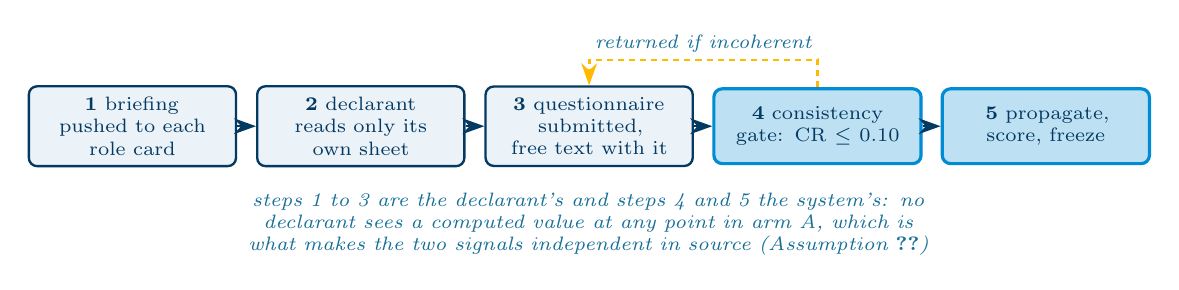
\begin{tikzpicture}[x=1cm, y=1cm, font=\scriptsize,
    phase/.style = {bloc, text width=2.35cm, minimum height=0.95cm},
    sys/.style  = {blocFort, text width=2.35cm, minimum height=0.95cm}]

\node[phase] (s1) at (1.55, 0) {\textbf{1} briefing\\pushed to each\\role card};
\node[phase] (s2) at (4.45, 0) {\textbf{2} declarant\\reads only its\\own sheet};
\node[phase] (s3) at (7.35, 0) {\textbf{3} questionnaire\\submitted,\\free text with it};
\node[sys]  (s4) at (10.25, 0) {\textbf{4} consistency\\gate:
                                $\mathrm{CR} \le 0.10$};
\node[sys]  (s5) at (13.15, 0) {\textbf{5} propagate,\\score, freeze};

\foreach \i/\j in {1/2, 2/3, 3/4, 4/5} \draw[fleche] (s\i) -- (s\j);
\draw[flecheCoupee] (s4.north) -- (10.25, 0.85) -- (7.35, 0.85) -- (s3.north);
\node[etiquette, anchor=south] at (8.8, 0.85) {returned if incoherent};

\node[etiquette, anchor=north, text width=12.5cm] at (7.35, -0.75)
     {steps 1 to 3 are the declarant's and steps 4 and 5 the system's: no declarant sees a
      computed value at any point in arm~A, which is what makes the two signals independent
      in source (Assumption~\ref{as:sincerity})};

\end{tikzpicture}
\caption[One turn of the protocol]{What happens inside a single turn. The dashed arc is the
consistency gate returning an incoherent questionnaire; it is the only feedback a declarant
receives, and it carries no information about the computed state.}
\label{fig:protocol_clock}
\end{figure} T0 is a training turn used to verify that every
declarant can complete the questionnaire inside ten minutes with the consistency gate
active; its declarations are retained in the record but excluded from every analysis. The
eighteen campaign turns run at two per day, morning and late afternoon, over nine working
days. One game turn represents one real month, from September 2020 to February 2022, with
real durations converted into engine hours at a fixed rate so that documented figures such as
twelve to twenty-five week supplier lead times or a six-day canal blockage retain their true
magnitude inside an eighteen-turn game.

\subsection*{Frozen Artefacts}

Four artefacts were frozen before T0 and are the reference against which any later analysis
is checked: the scenario definition with its twelve calibrated events and their turn
assignments; the data pack of public time series, with a SHA-256 hash recorded per file; the
role cards, one per node, each stating only what that declarant may know; and the hypothesis
register H1 to H6 with its numeric thresholds. Any analysis not derivable from the register
is labelled exploratory in the reporting.

\subsection*{Controls}

\begin{itemize}
    \item \emph{Isolation.} Each declarant sees only its own role sheet, its own turn
    briefing and its own questionnaire. Dashboards, scores, the network view and other
    declarants' material stay hidden until the debrief. In the executed campaign this is
    enforced by the harness, which gives each agent a private working directory, rather than
    by instruction.
    \item \emph{Placebo sheets.} A false de-escalation notice is handed to the avionics
    integrator at T9 and to the wafer supplier at T15. A declared urgency that follows the
    placebo is reflecting the sheet rather than a reading of the situation.
    \item \emph{Weak-signal turn.} At T4 the press briefing mentions a tension with no
    engine event behind it, which measures who reacts to media noise alone. This is also the
    turn on which the arm B treatment first becomes visible, so the two effects are
    deliberately not separated on that turn and the arm A control is what isolates them.
    \item \emph{Role assignment.} The two most information-heavy nodes, the foundry and
    the distributor, are assigned away from the most supply-chain-experienced participants,
    so that a role effect cannot be confounded with an expertise effect.
    \item \emph{Journal.} Every deviation from protocol is logged the same day.
\end{itemize}

\subsection*{Contingencies Arbitrated in Advance}

Three contingencies were decided before the campaign rather than improvised under time
pressure. The campaign truncates at T16 if it overruns by more than two turns, rather than
rushing the remaining responses. It drops to one turn per day if the questionnaire exceeds
ten minutes at the training turn. Any absence, or any unresolved consistency failure, is
carried forward unchanged and excluded from the reactivity analyses.

\subsection*{Declaration Record Format}

Each declaration is one JSON record per node per turn, carrying the turn index, the six
bipolar pairwise comparisons, the four severity scores, the derived criteria weights, the
principal eigenvalue with its consistency index and consistency ratio, a flag for whether the
consistency gate passed, the number of attempts, the raw and smoothed declared urgency, and a
free-text note. Arm B adds one field, \texttt{influence\_prediction}, taking one of four
values: no influence, confirms, revised upward, or revised downward. The format is otherwise
identical between arms, which is what makes them comparable.

\subsection*{Deviations Recorded in the Executed Campaign}

Two are on record. One node submitted turn 1 twice; the first submission is retained and the
duplicate discarded, which is why the arm B analysis reports 96 declarations from 97 raw
records. Arm B ran to T11 rather than T18, so its forecast log covers turns 4 to 12 against
turns 4 to 18 in arm A; all arm B comparisons in this thesis are therefore made over the
turns actually recorded, and the arm A scoring uses its own full range.


\subsection{Scenario and Network}
\label{app:scenario_detail}

The campaign, presented to participants under the cover story \emph{Programme H\'ELIOS},
replays the 2020 to 2022 semiconductor shortage over eighteen weekly game turns plus a
training turn. The supply network has eight nodes, one per participant, anchored on the real
actor types of the crisis (Table~\ref{tab:helios_network}).

Figure~\ref{fig:helios_network_coefficients} gives the network with its per-arc coefficients,
$\gamma$ attenuating demand as it descends and $\beta$ amplifying risk as it ascends. NovaFab
at rank 4 is the expected bottleneck, and the dashed arc into Meridian is the inert backup arc
of Section~\ref{sec:model_prop}: it appears in the diagram and carries nothing, which is the
point of including it.

One game turn represents one real month, with real durations converted into engine hours at a
fixed rate so that documented figures keep their true magnitude inside an eighteen-turn game.
Figure~\ref{fig:helios_timeline} lays the campaign out: five acts drawn from the documented
chronology, and the turn on which each calibrated event lands.

\begin{figure}[htbp]
\centering
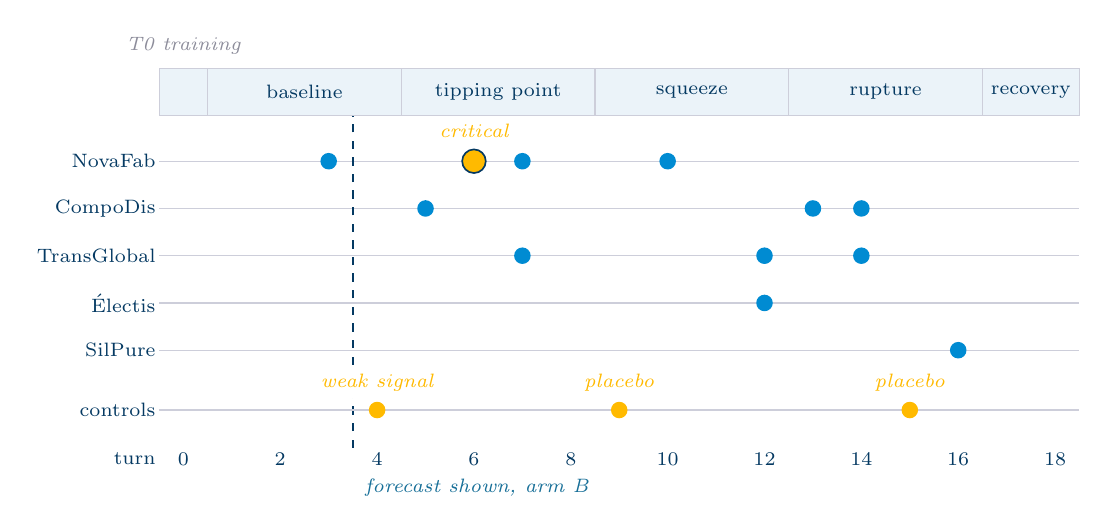
\begin{tikzpicture}[x=1cm, y=1cm, font=\scriptsize]

%% Echelle : 0,615 cm par tour, decalee de 2,75 pour laisser la place aux
%% intitules de voie. Les coordonnees sont calculees en ligne.

%% Les cinq actes, plus le tour d'entrainement.
\foreach \a/\b/\nom in {-0.5/0.5/{}, 0.5/4.5/baseline, 4.5/8.5/{tipping point},
                        8.5/12.5/squeeze, 12.5/16.5/rupture, 16.5/18.5/recovery} {
  \fill[altenBlueBg] ({2.75+0.615*\a}, 0.44) rectangle ({2.75+0.615*\b}, 1.04);
  \draw[altenGreyLine, line width=0.5pt]
       ({2.75+0.615*\a}, 0.44) rectangle ({2.75+0.615*\b}, 1.04);
  \node[text=altenNavy] at ({2.75+0.615*0.5*(\a+\b)}, 0.74) {\nom};
}
\node[font=\scriptsize\itshape, text=altenGreyText, anchor=south]
     at ({2.75+0.615*0}, 1.10) {T0 training};

%% Les cinq voies de noeud.
\foreach \i/\nom in {0/NovaFab, 1/CompoDis, 2/TransGlobal, 3/{\'Electis}, 4/SilPure} {
  \node[text=altenNavy, anchor=east] at (2.52, {-0.14-0.60*\i}) {\nom};
  \draw[altenGreyLine, line width=0.5pt]
       ({2.75-0.615*0.5}, {-0.14-0.60*\i}) -- ({2.75+0.615*18.5}, {-0.14-0.60*\i});
}

%% Les douze evenements calibres, a leur tour et sur leur voie.
\foreach \t/\i in {3/0, 7/0, 10/0, 5/1, 13/1, 14/1, 7/2, 12/2, 14/2, 12/3, 16/4}
  \fill[altenAzure] ({2.75+0.615*\t}, {-0.14-0.60*\i}) circle (0.105);

%% L'accident critique, seul de sa gravite.
\fill[altenOchreDark] ({2.75+0.615*6}, -0.14) circle (0.15);
\draw[altenNavy, line width=0.6pt] ({2.75+0.615*6}, -0.14) circle (0.15);
\node[etiquette, anchor=south, text=altenOchreDark] at ({2.75+0.615*6}, 0.06) {critical};

%% Le tour ou la prevision devient visible en bras B.
\draw[altenNavy, line width=0.8pt, dashed]
     ({2.75+0.615*3.5}, -3.78) -- ({2.75+0.615*3.5}, 0.44);
\node[etiquette, anchor=west] at ({2.75+0.615*3.6}, -4.28) {forecast shown, arm B};

%% La voie des controles du protocole : ils ont un tour comme les evenements.
\node[text=altenNavy, anchor=east] at (2.52, -3.30) {controls};
\draw[altenGreyLine, line width=0.5pt]
     ({2.75-0.615*0.5}, -3.30) -- ({2.75+0.615*18.5}, -3.30);
\foreach \t/\nom in {4/{weak signal}, 9/{placebo}, 15/{placebo}} {
  \fill[altenOchreDark] ({2.75+0.615*\t}, -3.30) circle (0.105);
  \node[etiquette, anchor=south, text=altenOchreDark] at ({2.75+0.615*\t}, -3.16) {\nom};
}

%% L'axe des tours.
\foreach \t in {0,2,4,6,8,10,12,14,16,18}
  \node[text=altenNavy] at ({2.75+0.615*\t}, -3.92) {\t};
\node[text=altenNavy, anchor=east] at (2.52, -3.92) {turn};

\end{tikzpicture}
\caption[The H\'ELIOS campaign, turn by turn]{The campaign over its nineteen turns: five acts
drawn from the documented chronology, and the twelve calibrated engine events on the node each
strikes, with the protocol's own controls on the lane beneath. Spot prices reach ten to forty
times catalogue during the squeeze; the rupture is a manufacturer cutting production by roughly
$40\%$ while the announced backup foundry turns out to have no spare capacity; the recovery
measures whether declared urgency lags the physical de-escalation. One event is of gravity
critical, the fab freeze at turn~6, and Table~\ref{tab:helios_events} names each event with its
real-world anchor.}
\label{fig:helios_timeline}
\end{figure}

\begin{figure}[htbp]
\centering
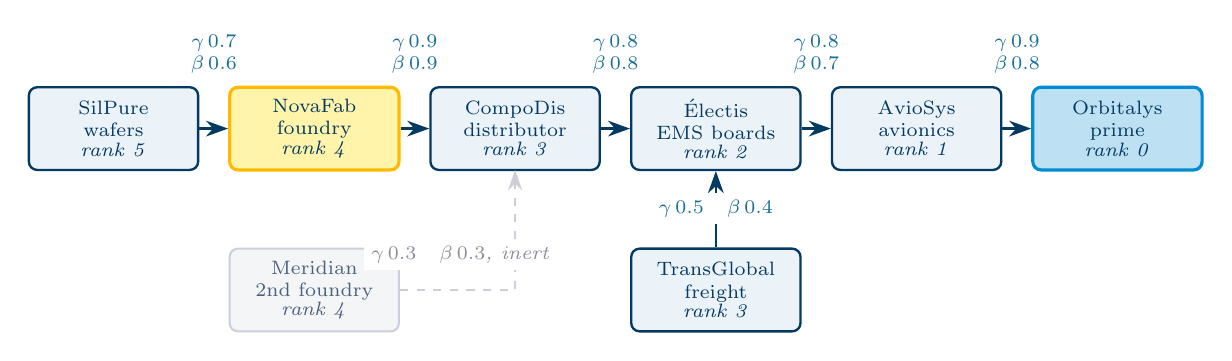
\begin{tikzpicture}[x=1cm, y=1cm, font=\scriptsize]

%% La chaine principale, du fournisseur de rang 5 au client de rang 0.
\node[bloc, minimum width=2.15cm, minimum height=1.05cm] (sil) at (1.15, 0)
     {SilPure\\wafers\\[-1pt]\textit{rank 5}};
\node[blocAlerte, minimum width=2.15cm, minimum height=1.05cm] (nov) at (3.70, 0)
     {NovaFab\\foundry\\[-1pt]\textit{rank 4}};
\node[bloc, minimum width=2.15cm, minimum height=1.05cm] (com) at (6.25, 0)
     {CompoDis\\distributor\\[-1pt]\textit{rank 3}};
\node[bloc, minimum width=2.15cm, minimum height=1.05cm] (ele) at (8.80, 0)
     {\'Electis\\EMS boards\\[-1pt]\textit{rank 2}};
\node[bloc, minimum width=2.15cm, minimum height=1.05cm] (avi) at (11.35, 0)
     {AvioSys\\avionics\\[-1pt]\textit{rank 1}};
\node[blocFort, minimum width=2.15cm, minimum height=1.05cm] (orb) at (13.90, 0)
     {Orbitalys\\prime\\[-1pt]\textit{rank 0}};

\foreach \a/\b in {sil/nov, nov/com, com/ele, ele/avi, avi/orb}
  \draw[fleche] (\a) -- (\b);

\foreach \x/\g/\bt in {2.425/0.7/0.6, 4.975/0.9/0.9, 7.525/0.8/0.8,
                       10.075/0.8/0.7, 12.625/0.9/0.8}
  \node[etiquette] at (\x, 0.95) {$\gamma\,\g$\\$\beta\,\bt$};

%% Les deux noeuds hors chaine principale.
\node[bloc, minimum width=2.15cm, minimum height=1.05cm] (tra) at (8.80, -2.05)
     {TransGlobal\\freight\\[-1pt]\textit{rank 3}};
\draw[fleche] (tra) -- (ele);
\node[etiquette] at (8.80, -1.02) {$\gamma\,0.5$ \; $\beta\,0.4$};

\node[blocPale, minimum width=2.15cm, minimum height=1.05cm] (mer) at (3.70, -2.05)
     {Meridian\\2nd foundry\\[-1pt]\textit{rank 4}};
\draw[flechePale, dashed] (mer.east) -- (6.25, -2.05) -- (6.25, -0.525);
\node[etiquette, text=altenGreyText] at (5.55, -1.60)
     {$\gamma\,0.3$ \; $\beta\,0.3$, inert};

\end{tikzpicture}
\caption[The H\'ELIOS network and its per-arc coefficients]{The eight campaign nodes,
$\gamma$ attenuating demand as it descends towards suppliers and $\beta$ amplifying risk as it
ascends towards Orbitalys, the final customer. NovaFab, in ochre, is the expected bottleneck.
The dashed arc into Meridian is the announced plan~B: it appears in the graph and carries
nothing.}
\label{fig:helios_network_coefficients}
\end{figure}

The twelve calibrated engine events driving the crisis are listed in
Table~\ref{tab:helios_events}, with the turn numbers as recorded in the campaign databases.
One encoding choice shapes what the scenario can test: the Texas freeze is modelled as a
production accident,
which triggers the engine's Bayesian revision of the failure probability, a recovery clock
and a severity ratchet, rather than as a capacity loss, which would only reduce storage
volume. A hot shutdown of a fabrication line is mechanically closer to the former.



\subsection{Protocol Integrity and Controls}
\label{sec:methods_controls}

The protocol was frozen before the first turn. Participants see only their own role sheet and
questionnaire; dashboards and scores stay hidden until the debrief, and no discussion between
roles is allowed. Three controls sit on the campaign lane of
Figure~\ref{fig:helios_timeline}. The two placebo sheets each hand one node a false
de-escalation, so a declared urgency that follows the sheet is reflecting the sheet rather than
a reading of the situation. The weak-signal turn has the press mention a tension with no engine
event behind it, which measures who reacts to media noise alone. Beyond those, roles are
assigned so that the two most information-heavy nodes do not go to the most experienced
participants, keeping a role effect from being confounded with an expertise effect, every
deviation is logged the same day in a campaign journal, and any analysis outside the
pre-registered register of Section~\ref{sec:hypotheses} is labelled exploratory.

%% ═══════════════════════════════════════════════════════════════════════════

\section{Full Scoring Tables}
\label{app:calibration}

Every value in this appendix is written by the derivation script of
Section~\ref{sec:methods_repro} and is reproduced here in full, so that the summary tables
of Section~\ref{sec:Results} can be checked against the complete output.

\subsection*{Turn to ISO Week Mapping}

The campaign runs from ISO week 2026-S31 at T0 to 2026-S49 at T18, one turn per week. The
outcome window of a forecast issued at turn $t$ with horizon $h$ therefore spans weeks
$t+1$ to $t+h$ inclusive.

\subsection*{Arm A, Production Outcome Definition}

Table~\ref{tab:app_armA_full} gives every quantity behind the summary of
Section~\ref{sec:res_armA_scored}, at all four horizons, including the confusion matrix at
the pre-registered threshold and the climatological Brier score the skill is measured
against.

\begin{table}[htbp]
\centering
\caption{Complete arm A scoring, production outcome definition}
\label{tab:app_armA_full}
\small
\begin{tabularx}{\linewidth}{l >{\centering\arraybackslash}X >{\centering\arraybackslash}X >{\centering\arraybackslash}X >{\centering\arraybackslash}X}
\toprule
\textbf{Quantity} & \textbf{h = 1} & \textbf{h = 2} & \textbf{h = 3} & \textbf{h = 4} \\
\midrule
Observations & 120 & 120 & 120 & 120 \\
Positive outcomes & 2 & 4 & 5 & 6 \\
Base rate & 0.017 & 0.033 & 0.042 & 0.050 \\
\midrule
AUC & 0.555 & 0.372 & 0.428 & 0.485 \\
AUC 95\% CI, lower & 0.470 & 0.258 & 0.315 & 0.389 \\
AUC 95\% CI, upper & 0.639 & 0.492 & 0.546 & 0.583 \\
PR-AUC & 0.027 & 0.031 & 0.041 & 0.054 \\
\midrule
Brier score & 0.130 & 0.166 & 0.191 & 0.207 \\
Brier, climatology & 0.016 & 0.032 & 0.040 & 0.047 \\
Brier skill & $-6.93$ & $-4.14$ & $-3.77$ & $-3.36$ \\
\midrule
True positives at $0.5$ & 0 & 0 & 0 & 0 \\
False positives at $0.5$ & 15 & 18 & 20 & 21 \\
False negatives at $0.5$ & 2 & 4 & 5 & 6 \\
True negatives at $0.5$ & 103 & 98 & 95 & 93 \\
\bottomrule
\end{tabularx}
\end{table}

\subsection*{Arm A, Naive Outcome Definition}

The naive definition counts any non-reverted event recorded on the node, regardless of
gravity, and ignores milestones entirely. It is scorable on the 75 node-turns for which the
node has at least one event in its history. Table~\ref{tab:app_wrong_target} repeats the
scoring under that definition, and the contrast with
Table~\ref{tab:app_armA_full} is the measurement reported in
Section~\ref{sec:res_target_trap}.

\begin{table}[htbp]
\centering
\caption{Complete arm A scoring, naive outcome definition}
\label{tab:app_wrong_target}
\small
\begin{tabularx}{\linewidth}{l >{\centering\arraybackslash}X >{\centering\arraybackslash}X >{\centering\arraybackslash}X >{\centering\arraybackslash}X}
\toprule
\textbf{Quantity} & \textbf{h = 1} & \textbf{h = 2} & \textbf{h = 3} & \textbf{h = 4} \\
\midrule
Observations & 75 & 75 & 75 & 75 \\
Positive outcomes & 11 & 19 & 25 & 29 \\
Base rate & 0.147 & 0.253 & 0.333 & 0.387 \\
AUC & 0.603 & 0.601 & 0.545 & 0.484 \\
Brier score & 0.155 & 0.248 & 0.337 & 0.389 \\
Brier skill & $-0.24$ & $-0.31$ & $-0.52$ & $-0.64$ \\
\bottomrule
\end{tabularx}
\end{table}

\subsection*{Right-Censoring Sensitivity}

Dropping every forecast whose observation window would extend past the final campaign turn
leaves the four-week scoring on 88 observations with 2 positives. The result does not
improve: the operating point remains 0 true positives against 16 false positives, and the
Brier skill moves from $-3.36$ to $-7.82$. Censoring is not the explanation for the confident
tail.

\subsection*{The Confident Tail, Forecast by Forecast}

Table~\ref{tab:app_confident} lists every arm A forecast announcing a four-week probability
of at least $0.5$. The rightmost column is the milestone-miss probability that the model
reports alongside it. The two never differ by more than $0.020$, which is the evidence that
the confident tail is the milestone channel and nothing else. None of the twenty-one was
followed by the predicted outcome under the production definition, which is what the Outcome
column reports; five of them were under the original-commitment definition of
Table~\ref{tab:app_milestones_original}.

\begin{table}[htbp]
\centering
\caption{Every arm A forecast at or above $0.5$ at four weeks}
\label{tab:app_confident}
\small
\begin{tabularx}{\linewidth}{c >{\raggedright\arraybackslash}p{3.4cm} >{\centering\arraybackslash}X >{\centering\arraybackslash}X >{\centering\arraybackslash}X}
\toprule
\textbf{Turn} & \textbf{Node} & \textbf{$p$ (4 weeks)} & \textbf{$p$ (milestone miss)} &
\textbf{Outcome} \\
\midrule
T5  & AvioSys Int\'egration & 0.898 & 0.880 & none \\
T6  & CompoDis Europe & 0.996 & 0.996 & none \\
T7  & CompoDis Europe & 1.000 & 1.000 & none \\
T8  & CompoDis Europe & 1.000 & 1.000 & none \\
T8  & NovaFab Semiconductors & 0.866 & 0.846 & none \\
T8  & Orbitalys & 1.000 & 1.000 & none \\
T9  & NovaFab Semiconductors & 1.000 & 1.000 & none \\
T9  & Orbitalys & 1.000 & 1.000 & none \\
T10 & AvioSys Int\'egration & 0.900 & 0.884 & none \\
T10 & NovaFab Semiconductors & 1.000 & 1.000 & none \\
T10 & Orbitalys & 1.000 & 1.000 & none \\
T11 & AvioSys Int\'egration & 0.898 & 0.884 & none \\
T11 & Orbitalys & 1.000 & 1.000 & none \\
T11 & TransGlobal Fret & 0.854 & 0.838 & none \\
T12 & Orbitalys & 1.000 & 1.000 & none \\
T13 & \'Electis EMS & 1.000 & 1.000 & none \\
T15 & AvioSys Int\'egration & 0.896 & 0.884 & none \\
T17 & AvioSys Int\'egration & 0.894 & 0.884 & none \\
T17 & CompoDis Europe & 0.998 & 0.998 & none \\
T18 & CompoDis Europe & 1.000 & 1.000 & none \\
T18 & Meridian Semi & 0.704 & 0.690 & none \\
\bottomrule
\end{tabularx}
\end{table}

Set against the registry, ten of the eighteen campaign milestones completed, eight remained
active, and none was abandoned. Exactly one was still open past a deadline that had fallen
inside the campaign. Every other node for which a near-certain miss was announced delivered,
though five of those deliveries arrived after the deadline originally committed to, which the
registry does not record because a replanning overwrites the deadline it stores.
Table~\ref{tab:app_milestones_original} gives that reading milestone by milestone.

\subsection*{Arm B, Per-Node Influence Record}

Table~\ref{tab:app_armB_t4} records the first-exposure turn node by node, which is the
observation behind the result of Section~\ref{sec:res_armB}.

\begin{table}[htbp]
\centering
\caption{Arm B at turn 4, node by node}
\label{tab:app_armB_t4}
\small
\begin{tabularx}{\linewidth}{>{\raggedright\arraybackslash}p{5.0cm} X}
\toprule
\textbf{Node} & \textbf{Recorded influence of the displayed forecast} \\
\midrule
AvioSys Int\'egration & Confirms existing assessment \\
CompoDis Europe & Revised downward \\
\'Electis EMS & Confirms existing assessment \\
Meridian Semi & Confirms existing assessment \\
NovaFab Semiconductors & Revised downward \\
Orbitalys & Revised downward \\
SilPure Materials & Revised downward \\
TransGlobal Fret & Revised downward \\
\midrule
\textbf{Total} & \textbf{5 downward, 3 confirmed, 0 upward, 8 of 8 responding} \\
\bottomrule
\end{tabularx}
\end{table}

NovaFab is the node that carries the scenario's critical accident event two turns later, at
turn 6.

\subsection*{Milestones Against Their Original Commitment}
\label{app:milestones_original}

Table~\ref{tab:app_milestones_original} is the counterpart of the registry counts above. It
lists every milestone whose \emph{original} deadline falls inside the campaign, together with
the turn at which it was actually delivered in arm A and in the closed-loop arm of
Section~\ref{sec:res_repair}. Seven further milestones carry original deadlines at turns 20
to 22 and are therefore unobservable within a nineteen-turn campaign; they are excluded here
rather than counted as met.

\begin{table}[htbp]
\centering
\caption{The eleven milestones observable within the campaign, judged against the deadline
first committed to}
\label{tab:app_milestones_original}
\small
\begin{tabularx}{\linewidth}{>{\raggedright\arraybackslash}p{4.6cm} >{\centering\arraybackslash}X >{\centering\arraybackslash}X >{\centering\arraybackslash}X >{\centering\arraybackslash}X}
\toprule
\textbf{Milestone} & \textbf{Original deadline} & \textbf{Arm A delivery} &
\textbf{Closed-loop deadline} & \textbf{Closed-loop verdict} \\
\midrule
Orbitalys, H\'ELIOS-1 delivery & T8 & T14 & T14 & Missed \\
Orbitalys, H\'ELIOS-2 delivery & T16 & not delivered & T19 & Missed \\
AvioSys, avionics batch 1 & T6 & T6 & T6 & Met \\
AvioSys, avionics batch 2 & T11 & T12 & T12 & Missed \\
AvioSys, avionics batch 3 & T16 & T18 & T18 & Missed \\
\'Electis, H\'ELIOS series A & T6 & T6 & T6 & Met \\
\'Electis, H\'ELIOS series B & T13 & T14 & T13 & \textbf{Met} \\
CompoDis, component cover S1 & T9 & T9 & T11 & \textbf{Missed} \\
TransGlobal, annual flow contract & T12 & T12 & T12 & Met \\
NovaFab, H\'ELIOS wafer allocation & T10 & T11 & T12 & Missed \\
SilPure, annual wafer contract & T15 & T14 & T15 & Met \\
\midrule
\textbf{Met on original commitment} & & \textbf{5 of 11} & & \textbf{5 of 11} \\
\bottomrule
\end{tabularx}
\end{table}

The two rows set in bold are the only ones on which the arms differ. The closed loop saved
the \'Electis series B, which slipped in arm A, and replanned the CompoDis S1 cover, which
arm A met on its original date. Every other difference between the arms is a replanning that
re-dated a milestone arm A also delivered late: an announced slip rather than a discovered
one, which is not nothing and is not a save.

Under this definition of truth, five of the twenty-one confident arm A forecasts of
Table~\ref{tab:app_confident} are followed by a missed original commitment within four weeks,
at T8 and T9 on NovaFab, T10 and T15 on AvioSys, and T12 on Orbitalys, against none under the
registry's current-deadline reading.

\subsection*{Arm A Rescored After Repair}
\label{app:repair_tables}

Tables~\ref{tab:app_repair_before} to \ref{tab:app_repair_after} give the complete scoring
behind Table~\ref{tab:repair_scores}. All three score the same 120 forecasts against the
original-commitment target, censored points excluded, so the observation counts are identical
across the three and only the model differs. The first is the frozen campaign as run, the
second applies the structural repair of Equation~\ref{eq:completion_repaired} alone, and the
third adds the progress-uncertainty term.

\begin{table}[htbp]
\centering
\caption{Arm A before repair, original-commitment target}
\label{tab:app_repair_before}
\small
\begin{tabularx}{\linewidth}{l *{4}{>{\centering\arraybackslash}X}}
\toprule
\textbf{Quantity} & \textbf{h = 1} & \textbf{h = 2} & \textbf{h = 3} & \textbf{h = 4} \\
\midrule
Observations & 112 & 104 & 96 & 90 \\
Positive outcomes & 7 & 14 & 20 & 26 \\
Base rate & 0.062 & 0.135 & 0.208 & 0.289 \\
\midrule
Brier score & 0.1335 & 0.1969 & 0.2728 & 0.3190 \\
Brier skill & $-1.278$ & $-0.690$ & $-0.654$ & $-0.553$ \\
AUC & 0.736 & 0.636 & 0.641 & 0.654 \\
AUC 95\% CI & [0.49, 0.93] & [0.37, 0.87] & [0.39, 0.85] & [0.42, 0.85] \\
PR-AUC & 0.163 & 0.205 & 0.266 & 0.353 \\
\bottomrule
\end{tabularx}
\end{table}

\begin{table}[htbp]
\centering
\caption{Arm A after the structural repair alone}
\label{tab:app_repair_struct}
\small
\begin{tabularx}{\linewidth}{l *{4}{>{\centering\arraybackslash}X}}
\toprule
\textbf{Quantity} & \textbf{h = 1} & \textbf{h = 2} & \textbf{h = 3} & \textbf{h = 4} \\
\midrule
Brier score & 0.0965 & 0.1633 & 0.2243 & 0.2613 \\
Brier skill & $-0.646$ & $-0.401$ & $-0.360$ & $-0.272$ \\
AUC & 0.793 & 0.671 & 0.657 & 0.721 \\
AUC 95\% CI & [0.60, 0.95] & [0.51, 0.88] & [0.47, 0.87] & [0.54, 0.92] \\
PR-AUC & 0.355 & 0.305 & 0.355 & 0.484 \\
\bottomrule
\end{tabularx}
\end{table}

\begin{table}[htbp]
\centering
\caption{Arm A after the structural repair and the progress-uncertainty term}
\label{tab:app_repair_after}
\small
\begin{tabularx}{\linewidth}{l *{4}{>{\centering\arraybackslash}X}}
\toprule
\textbf{Quantity} & \textbf{h = 1} & \textbf{h = 2} & \textbf{h = 3} & \textbf{h = 4} \\
\midrule
Brier score & 0.0988 & 0.1593 & 0.2120 & 0.2499 \\
Brier skill & $-0.687$ & $-0.367$ & $-0.286$ & $-0.216$ \\
AUC & 0.729 & 0.634 & 0.602 & 0.584 \\
AUC 95\% CI & [0.56, 0.95] & [0.42, 0.83] & [0.29, 0.85] & [0.21, 0.87] \\
PR-AUC & 0.195 & 0.228 & 0.299 & 0.385 \\
\bottomrule
\end{tabularx}
\end{table}

The confidence intervals are cluster bootstraps resampling whole nodes rather than individual
node-weeks, because forecasts on one node are strongly correlated and an i.i.d.\ bootstrap
would understate the width. They are wide enough at every horizon to contain the AUC of every
other table in this group, which is why the AUC movements between the three are reported as
uninterpretable rather than as gains or losses, while the Brier skill movements, which do not
depend on the size of the positive class in the same way, are reported as measured.

\subsection*{Distribution of the Milestone Probability}
\label{app:binarity}

Table~\ref{tab:app_binarity} counts how many of the 120 milestone-miss probabilities fall at
the extremes rather than in a usable band, which is the measurement behind the
progress-uncertainty term of Section~\ref{sec:res_repair}.

\begin{table}[htbp]
\centering
\caption{Degeneracy of the milestone-miss probability, 120 forecasts}
\label{tab:app_binarity}
\small
\begin{tabularx}{\linewidth}{>{\raggedright\arraybackslash}p{5.2cm} >{\centering\arraybackslash}X >{\centering\arraybackslash}X >{\centering\arraybackslash}X}
\toprule
\textbf{Model} & \textbf{Exactly 0 or 1} & \textbf{In $(0.05, 0.95)$} &
\textbf{Forecasts $\ge 0.5$ at 4 weeks} \\
\midrule
Frozen campaign as run & 102 (85.0\%) & 14 & 21 \\
Structural repair alone & 89 (74.2\%) & 10 & 10 \\
Structural repair with progress uncertainty & 86 (71.7\%) & 17 & 10 \\
\bottomrule
\end{tabularx}
\end{table}

The structural repair alone reduces the count of extreme values but not the usable band: it
removes eleven false certainties without producing gradations. The progress-uncertainty term
is what widens the usable band, from 10 forecasts to 17. Neither is sufficient, and $71.7\%$
of the probabilities remain degenerate.

\section{Satellite Capacity Estimation: Protocol and Data}
\label{app:volume}

This appendix records the operational detail behind the opening of
Section~\ref{sec:res_volume}, so that its measurements can be audited or repeated.

\subsection*{Data Sources}

All sources are public French open-data services, accessed over standard web map and feature
services and cached on disk so that a re-run does not depend on service availability.
Table~\ref{tab:app_volume_sources} lists each one with the role it plays in the pipeline.

\begin{table}[htbp]
\centering
\caption{Data sources of the capacity pipeline}
\label{tab:app_volume_sources}
\small
\begin{tabularx}{\linewidth}{>{\raggedright\arraybackslash}p{4.0cm} X}
\toprule
\textbf{Source} & \textbf{Use} \\
\midrule
Orthophotography, 20~cm & Primary imagery for detection and segmentation \\
Orthophotography, 5 to 10~cm & Partial coverage, used only for the resolution control of
Figure~\ref{fig:volume_resolution} \\
LiDAR surface model & Building height where available, delivered as 32-bit float raster \\
National topographic database & Building footprints and, where populated, height \\
Classified installations register & Declared storage volume, used only to calibrate the
fill factor \\
\bottomrule
\end{tabularx}
\end{table}

All geometry is handled in the national metric projection, in which the ground sample
distance is exactly the bounding-box width in metres divided by the image width in pixels
rather than an approximation.

\subsection*{Calibration of the Fill Factor}

The fill factor relates declared storage volume to the geometric envelope. For each site in
the regulatory register, the nearest building footprint is matched, the geometric volume is
computed as footprint area times eaves height, and the ratio of declared to geometric volume
is recorded. Ratios outside $[0.05, 20]$ are discarded as either an aberrant declaration or a
mismatched building. The production constant of $0.80$ is attributed in the source to a
median over 122 matched sites with an interquartile range of $[0.52, 1.22]$.

That run cannot be reproduced from the retained artifacts, and the discrepancy is recorded
here in full. The calibration script writes its detailed output to a file that is not present
in the repository, so the only auditable sample is the 68-site corpus retained for other
purposes. Recomputing the identical ratio over those 68 sites gives a median of $0.966$, an
interquartile range of $[0.80, 2.00]$, and $47\%$ of sites inside the $[0.7, 1.4]$ band,
against the $70\%$ the calibration script itself prints as its acceptance target. The
available evidence does not distinguish between a biased remnant sample and an understated
production constant. Recollecting the register cleanly, with the departmental loop and
pagination the script provides, and rederiving the factor, is the resolution.

One matching rule is worth recording because it changes the answer materially. Only the
largest building within the search radius is matched, and neighbouring buildings are not
summed: summing them moves the median ratio from $0.80$ to $0.58$, because a declared volume
belongs to one warehouse while the footprints of a whole industrial estate do not.

\subsection*{Annotation Protocol}

The dataset comprises 442 georeferenced image chips, each retained at a single location, a
single resolution and a single vintage, with a sidecar file recording its geographic
transform. Of these, 351 form the training split and 91 the validation split.

Annotators mark one class, the continuous extent of facade served by a dock apron, and the
following rules apply.

\begin{itemize}
    \item Mark an equipped facade even where no vehicle is parked. The apron and canopy
    remain visible, and a facade annotated only when a vehicle is present teaches the model
    to detect vehicles.
    \item Do not annotate a trailer holding yard that is not adjacent to a wall.
    \item Do not annotate an aeronautical tarmac or a small-business forecourt. Both are
    paved and deep but serve no docks.
    \item A facade without docks is annotated empty. That is a useful negative, not an
    omission, and roughly 40\% of the target sample is negative by design.
    \item Ignore everything above the facade line, which is roof. Rooflights and sawtooth
    roofs are perfectly periodic and are the principal source of false positives.
    \item Annotate every visible dock zone in a chip regardless of which building owns it.
    Ownership is resolved downstream by geometric clipping, so the model is never asked to
    infer it from pixels, and annotating a zone in one chip but not in the overlapping
    neighbour would give the model two contradictory labels for the same ground.
\end{itemize}

Sampling is stratified by footprint area across three bands, roughly 1\,500 to
5\,000~m\textsuperscript{2}, 5\,000 to 20\,000~m\textsuperscript{2} and above
20\,000~m\textsuperscript{2}, and across five site categories covering small enterprises,
aerospace, refrigerated, very large and retail distribution. An unstratified random draw
over-represents large warehouses, and the model inherits that bias.

\subsection*{Training Configuration}

The model is a segmentation network trained from pre-trained weights at a $640$~pixel input
size, with rotation augmentation over the full circle, horizontal and vertical flips, and
scale jitter. Rotation invariance is obtained by augmentation rather than by geometric
rectification of the facade, which is what allows the model to accept any building shape and
orientation without requiring a footprint as input. Training ran on CPU throughout, with no
GPU available, which is the practical reason the input size was not raised further and the
context for the negative resolution result of Table~\ref{tab:volume_training}.

\subsection*{Measured Facts Recorded for Reuse}

\begin{itemize}
    \item Empty bay contrast at verified locations: $0.18\sigma$, $0.22\sigma$ and
    $0.01\sigma$, against $5.3\sigma$ to $6.4\sigma$ at occupied bays on the same facades,
    over a full sweep of assumed apron depths from $0.3$~m to $20$~m.
    \item Dock pitch coherence between facades of the same building: $0.03$ to $0.05$~m,
    which provides a free quality control.
    \item Roof overhang beyond the footprint edge: $0$ to $14.4$~m. This is why the footprint
    edge is not the start of the apron, and it was the cause of an earlier defect in which
    rooflights were counted as bays.
    \item Trailer distance to building: median up to $126$~m on large platforms; at one site
    only 8 of 89 detected trailers lay within $26$~m. Trailers are not a proxy for docks.
    \item Zero-shot coverage before the learned model: 25 of 70 sites, or $36\%$.
    \item Prompt sensitivity of the promptable segmentation model used for site sampling: a
    prompt naming an industrial warehouse returns 88\,752~m\textsuperscript{2}, some 45\% of
    the view, where a prompt naming a warehouse roof returns the
    13\,478~m\textsuperscript{2} of the roof itself. The first is useful for locating a site,
    the second for measuring it, and they are not interchangeable.
\end{itemize}

\subsection*{Licensing Constraint}

The detection and segmentation library used is distributed under a strong copyleft licence.
This has no consequence for internal research use, but it becomes determinative the moment
the capability is distributed or exposed over a network. The options are a commercial licence
from the vendor or replacement of the backbone with a permissively licensed equivalent. This
is recorded as a governance decision to be taken deliberately rather than discovered at
deployment.

%% ═══════════════════════════════════════════════════════════════════════════
\section{A Worked Example, End to End}
\label{app:worked}
%% ═══════════════════════════════════════════════════════════════════════════

Section~\ref{sec:math_framework} gives the model as equations and Section~\ref{sec:Results}
gives it as scores on a campaign. Neither shows a single number travelling through the whole
chain, which is what a reader needs to check that the equations mean what the prose
says they mean. This appendix carries one node through every stage: the six blocks into a
local urgency, that urgency along a three-node chain, the chain into a criticality ranking,
and the result against a declaration.

Every figure below is produced by the production code rather than computed by hand, using
the same functions the campaign ran, so the example cannot drift away from the system it
illustrates. The scenario is illustrative and is not drawn from either campaign.

\subsection{Stage 1: six blocks into a local urgency}

The node is a deep-tier supplier whose next milestone falls in nine days against a lead time
distributed $\mathcal{N}(11, 3)$, whose buffers are a third consumed, whose OEE stands at
$0.80$, and for which no node-level emissions data exists. Table~\ref{tab:worked_blocks}
gives the resulting block values and the survival factor each contributes to
Equation~\ref{eq:ur_local}.

\begin{table}[htbp]
\centering
\caption[Worked example: the six blocks]{The six blocks and their survival factors, all
weights at $\omega_m = 1$}
\label{tab:worked_blocks}
\small
\begin{tabularx}{\linewidth}{@{}l c c X@{}}
\toprule
\textbf{Block} & \textbf{$u_m$} & \textbf{$(1-u_m)^{\omega_m}$} & \textbf{Reading} \\
\midrule
$u_{\text{time}}$ & $0.62$ & $0.3800$ & Probability of missing the nine-day deadline \\
$u_{\text{cap}}$  & $0.35$ & $0.6500$ & Buffers a third consumed \\
$u_{\text{perf}}$ & $0.20$ & $0.8000$ & $1 - \text{OEE}$, with OEE at $0.80$ \\
$u_{\text{risk}}$ & $0.15$ & $0.8500$ & Expected unavailability over the horizon \\
$u_{\text{cost}}$ & $0.28$ & $0.7200$ & Operating cost drifting above nominal \\
$u_{\text{co2}}$  & absent & $1.0000$ & $\omega_m = 0$: the factor is neutral, not healthy \\
\midrule
\multicolumn{2}{@{}l}{Product of survivals} & $0.120931$ & \\
\multicolumn{2}{@{}l}{$U_{r,\text{local}} = 1 - \text{product}$} & $\mathbf{0.8791}$ & \\
\bottomrule
\end{tabularx}
\end{table}

The comparison that matters is with the aggregator the model rejects. A weighted average of
the same five available blocks gives $0.3200$. The two answers differ by more than half the
scale on identical inputs, and they differ because they answer different questions: the
average asks how stressed this node is on average, the noisy-OR asks how likely it is that
at least one mechanism ruptures. Only the second is the quantity a coordinator needs.

The gap widens at the boundary. Let the deadline pass, so $u_{\text{time}} = 1$ and the node
cannot become any later. The noisy-OR returns exactly $1.0000$, because the factor
$(1-1) = 0$ collapses the product whatever the other blocks read. The weighted average
returns $0.3960$, and would rank this node below a node that is mildly stressed on all six.
That is the compensatory failure of Section~\ref{sec:model_ur} in a single pair of numbers.

\subsection{Stage 2: propagation along a three-node chain}

Place the node as the deepest tier of a chain $s_2 \to s_1 \to \text{customer}$, with
upstream amplification $\beta_{s_2 s_1} = 0.70$ and $\beta_{s_1 c} = 0.50$. The two
downstream nodes are locally calm, at $U_{r,\text{local}} = 0.30$ and $0.10$.
Equation~\ref{eq:ur_prop} applied in topological order gives
\begin{align*}
    U_{r,s_2} &= 0.8791, \\
    U_{r,s_1} &= 1 - (1 - 0.30)\bigl(1 - 0.70 \times 0.8791\bigr) = 0.7307, \\
    U_{r,c}   &= 1 - (1 - 0.10)\bigl(1 - 0.50 \times 0.7307\bigr) = 0.4288 .
\end{align*}
\begin{figure}[htbp]
\centering
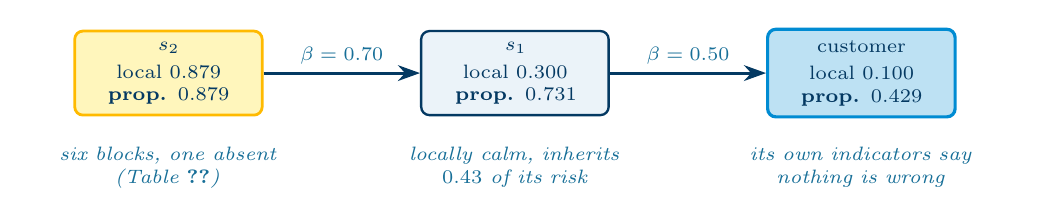
\begin{tikzpicture}[x=1cm, y=1cm, font=\scriptsize,
    nd/.style = {bloc, text width=2.1cm, minimum height=1.05cm}]

\node[nd, fill=altenOchrePale!55!white, draw=altenOchreDark, line width=1pt] (s2) at (1.6, 0)
     {$s_2$\\[2pt]local $0.879$\\\textbf{prop. $0.879$}};
\node[nd] (s1) at (6.0, 0) {$s_1$\\[2pt]local $0.300$\\\textbf{prop. $0.731$}};
\node[nd, blocFort] (c) at (10.4, 0) {customer\\[2pt]local $0.100$\\\textbf{prop. $0.429$}};

\draw[fleche, line width=1.1pt] (s2) -- node[etiquette, above] {$\beta = 0.70$} (s1);
\draw[fleche, line width=1.1pt] (s1) -- node[etiquette, above] {$\beta = 0.50$} (c);

\node[etiquette, anchor=north, text width=3.4cm] at (1.6, -0.85)
     {six blocks, one absent\\(Table~\ref{tab:worked_blocks})};
\node[etiquette, anchor=north, text width=3.4cm] at (6.0, -0.85)
     {locally calm, inherits\\$0.43$ of its risk};
\node[etiquette, anchor=north, text width=3.6cm] at (10.4, -0.85)
     {its own indicators say\\nothing is wrong};

\end{tikzpicture}
\caption[The worked chain]{The three-node chain of Stage~2. Each box carries the node's own
local urgency above and its propagated value below. The customer's local reading of $0.10$
becomes $0.43$ once two tiers of upstream risk arrive, which is the whole purpose of the
propagation.}
\label{fig:worked_chain}
\end{figure}

A node that is locally calm at $0.10$ therefore carries a propagated urgency of $0.43$,
entirely inherited from two tiers upstream. This is the whole purpose of the propagation: the
customer's own indicators say nothing is wrong, and something is.

The log-survival twin of Proposition~\ref{prop:logsurvival} can be checked on the same
figures. Equation~\ref{eq:logsurvival} gives $\ell_c = 0.5601$ at the customer, and
$1 - e^{-0.5601} = 0.4288$, which is $U_{r,c}$ to every digit shown. The twin is the same
recurrence in another coordinate, exactly as the proposition states.

\subsection{Stage 3: which node is the most critical}

The criticality index of Section~\ref{sec:criticality} shocks each active node to
$U_{r,\text{local}} = 1$ in turn and measures the rise at the customer. On this chain:

\begin{table}[htbp]
\centering
\caption[Worked example: criticality]{Effect of the worst local shock, measured at the
customer}
\label{tab:worked_crit}
\small
\begin{tabularx}{\linewidth}{@{}l c c c X@{}}
\toprule
\textbf{Shocked node} & \textbf{$U_{r,\text{local}}$} & \textbf{$U_{r,c}$ after} &
\textbf{$\Delta U_{r,c}$} & \textbf{Rank} \\
\midrule
$s_1$ & $0.30 \to 1.00$ & $0.5500$ & $+0.1212$ & 1st \\
$s_2$ & $0.88 \to 1.00$ & $0.4555$ & $+0.0267$ & 2nd \\
\bottomrule
\end{tabularx}
\end{table}

The result is worth pausing on, because it is counter-intuitive and it is correct. The most
urgent node, $s_2$ at $0.88$, is the \emph{least} critical of the two. Two effects combine.
Its risk is already almost entirely realised in the baseline, so forcing it to $1$ adds
little that the customer was not already exposed to. And what it adds is damped twice, once
by $\beta_{s_2 s_1} = 0.70$ and again by $\beta_{s_1 c} = 0.50$, while $s_1$ sits behind a
single arc. Urgency and criticality are therefore different questions, and a coordinator who
sorts the network by urgency alone will spend attention on the node that has least left to
lose.

Proposition~\ref{prop:saturation} can be seen on the same chain. Set every local urgency to
$1.0$, the state the campaign reaches on nine turns of nineteen. The baseline customer
urgency is then $1$, and shocking either node gives $\Delta U_{r,c} = +0.0000$ exactly. Both
nodes tie at zero, the ranking carries no information, and the log-survival key of
Proposition~\ref{prop:order} is what separates them again.

\subsection{Stage 4: the declaration, and the adequacy it produces}

Finally, the deep supplier's own coordinator fills the weekly questionnaire.
Table~\ref{tab:worked_adequacy} scores two declarations against the computed
$U_{r} = 0.8791$, using the default $\lambda_{\text{under}} = 2.25$,
$\lambda_{\text{over}} = 1.0$ and $\alpha = 0.88$.

\begin{table}[htbp]
\centering
\caption[Worked example: adequacy]{Two declarations against the same computed urgency}
\label{tab:worked_adequacy}
\small
\begin{tabularx}{\linewidth}{@{}c c c c c X@{}}
\toprule
\textbf{$U_d$} & \textbf{$F$} & \textbf{$H$} & \textbf{penalty} & \textbf{$A$} &
\textbf{Reading} \\
\midrule
$0.83$ & $0.0000$ & $0.0491$ & $0.1585$ & $83.6$ & A lucid coordinator, slightly optimistic \\
$0.40$ & $0.0000$ & $0.4791$ & $1.1774$ & $22.7$ & Hidden risk of nearly half the scale \\
\bottomrule
\end{tabularx}
\end{table}

The second row is the situation the whole instrument exists to surface. The node is at
$0.88$ and is reported at $0.40$; nothing in the declaration is a lie, and the coordinator
may sincerely believe it, which is Assumption~\ref{as:sincerity}. The adequacy score falls to $22.7$ and the hidden risk
$H = 0.479$ is what a supervising view would rank on. Note also what the first row shows: at
$U_d = 0.83$ against $U_r = 0.88$ the score is $83.6$ and not $95$, because
Proposition~\ref{prop:adequacy}(iv) makes the curve steepest near zero. Small
mis-declarations are penalised hard on purpose, since they are the ones still cheap to
correct.

%% ═══════════════════════════════════════════════════════════════════════════
\section{Register of Modelling Assumptions}
\label{app:assumptions}
%% ═══════════════════════════════════════════════════════════════════════════

A model is the set of commitments it makes, and those commitments are scattered through
Section~\ref{sec:Methods} at the point where each first becomes necessary. This appendix
collects them in one place so that a reader can weigh the whole set at once rather than
reconstruct it, and so that the ones this work could not test are as visible as the ones it
could.

Three statuses are used, and the distinction between the last two is the one that matters.
\emph{Tested} means the campaign produced evidence bearing on the assumption and
Section~\ref{sec:Results} reports it. \emph{Testable, untested} means an experiment within
reach of this design would bear on it and was not run, usually for want of events or time;
these are recoverable and Section~\ref{sec:future_work} carries them. \emph{Outside this
design} means no experiment this instrument can run would settle the question, so the
assumption is load-bearing and permanent until the design changes; these are the ones that
bound what the thesis may claim.

\subsection{The register}

Read down the status column first. It is the shorter question, and it decides how much
weight the rest of the row can carry.

\begin{longtable}{@{}p{0.5cm} p{4.1cm} p{2.0cm} p{7.6cm}@{}}
\caption[Register of modelling assumptions]{Every modelling assumption, where it is stated,
and what is known about it}
\label{tab:assumptions} \\
\toprule
& \textbf{Assumption} & \textbf{Status} & \textbf{If it fails} \\
\midrule
\endfirsthead
\multicolumn{4}{@{}l}{\small\itshape Table~\ref{tab:assumptions}, continued} \\
\toprule
& \textbf{Assumption} & \textbf{Status} & \textbf{If it fails} \\
\midrule
\endhead
\bottomrule
\endlastfoot

A1 & The six blocks are independent competing causes of rupture
(Assumption~\ref{as:noisyor}, Section~\ref{sec:model_ur})
& Tested
& Correlated blocks double-count a shared cause and the aggregate overstates urgency. The
direction is conservative: it errs towards alarm, never towards complacency.
Section~\ref{sec:res_armA} reports the observed inter-block correlations. \\
\addlinespace

A2 & The blocks are exchangeable up to their weights $\omega_m$
(Section~\ref{sec:model_ur})
& Tested, and false in detail
& $u_{\text{time}}$ is a frequentist probability and $u_{\text{cost}}$ an ordinal statement in
cardinal dress; no transfer function makes them equally informative. The aggregate is
therefore usable for ranking and for comparison against $U_d$, and is not a calibrated
probability. This is the reason no Brier score is reported on $U_r$ itself. \\
\addlinespace

A3 & The declaration is sincere (Assumption~\ref{as:sincerity},
Section~\ref{sec:model_adequacy})
& Outside this design
& Hidden risk stops measuring misperception and starts measuring what a declarant is willing
to write down. The two demand opposite interventions and are indistinguishable in this data.
Every behavioural reading in Section~\ref{sec:Results} rests on it. \\
\addlinespace

A4 & Language-model agents stand in for human declarants
(Section~\ref{sec:methods_arms})
& Outside this design
& Every statement about declaration behaviour applies to that population and not to
consultants. The mechanical findings are unaffected, since they concern code paths rather
than declarants. \\
\addlinespace

A5 & Lead times are lognormal by default, parameterised by moments
(Section~\ref{sec:model_mc})
& Testable, untested
& The tail of the completion-time distribution is misstated and $u_{\text{time}}$ with it.
The law is configurable per node, and normal-clipped and triangular alternatives are
implemented, so the sensitivity is measurable on frozen scenarios at low cost. \\
\addlinespace

A6 & Lead times are drawn independently across nodes
(Section~\ref{sec:model_mc})
& Outside this design
& A common shock, an energy crisis or a regional closure, correlates delays that the
simulation treats as independent, and the simulated completion distribution is too narrow.
Nothing in the campaign scenario could separate this from ordinary variance. \\
\addlinespace

A7 & The arc coefficients $\beta_{ji}$ and $\gamma_{ik}$ are known constants
(Section~\ref{sec:model_prop})
& Testable, untested
& Propagated urgency is misscaled. The coefficients are set by the scenario rather than
estimated from data, and estimating them from observed co-movement of node states is the
natural next study. \\
\addlinespace

A8 & Backup arcs carry neither propagation
(Section~\ref{sec:model_prop})
& Modelling choice, exercised
& A network with a real alternative supplier reads as more exposed than it is. The choice is
deliberate, since an unqualified backup is documentation rather than capacity, and the
campaign scenario exploits it on purpose. \\
\addlinespace

A9 & The Prospect Theory parameters transfer to supply chain coordinators,
$\lambda_{\text{under}} = 2.25$ and $\alpha = 0.88$
(Section~\ref{sec:model_adequacy})
& Testable, untested
& The adequacy score is miscalibrated as a governance instrument, though its ordering is
unaffected, since $A$ is monotone in the gap whatever the parameters
(Proposition~\ref{prop:adequacy}(ii)). Both are configurable per project and neither is
hard-coded. \\
\addlinespace

A10 & Local urgency follows a stationary AR(1)
(Section~\ref{sec:methods_forecast})
& Testable, untested
& The projected urgency path is wrong in shape, and with it every $p_h$. Nineteen turns is
short for a specification test, which is why the coefficient is clipped to $[0,0.98]$ rather
than trusted. \\
\addlinespace

A11 & Weeks are independent Bernoulli trials for the adverse-event rate
(Section~\ref{sec:methods_forecast})
& Testable, untested
& Clustered events, one incident producing three weeks of consequences, break independence
and the Beta posterior understates uncertainty. The prior strength of $N_0 = 26$ dominates
nineteen turns of data, which masks the effect here and would not on a longer campaign. \\
\addlinespace

A12 & The calibration service's outcome definition is the right target
(Section~\ref{sec:methods_scoring})
& Tested
& Every score in this thesis moves. This is the one assumption whose failure was measured
rather than argued: Section~\ref{sec:res_target_trap} scores identical forecasts against
three definitions and finds a spread wider than any modelling decision taken in this work. \\

\end{longtable}

\subsection{What the register says when read as a whole}

Twelve assumptions, of which three are tested, five are testable and untested, one is a
declared modelling choice, and three sit outside what this design can reach. That last group is the honest statement of the thesis's
boundary, and it has a shape: A3 and A4 both concern the declarant, and A6 concerns
correlation between nodes. What the instrument cannot see is people and common causes,
which is to say the two things a supply chain is made of besides its arithmetic.

\begin{figure}[htbp]
\centering
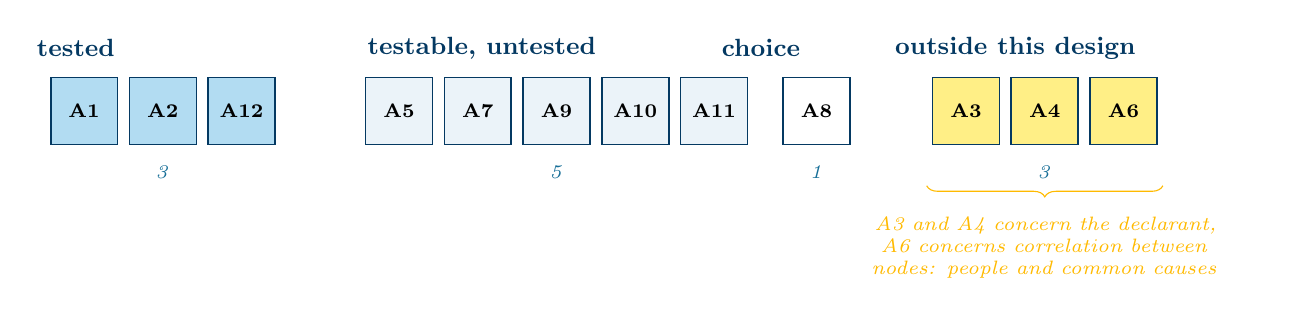
\begin{tikzpicture}[x=1cm, y=1cm, font=\scriptsize,
    st/.style = {minimum width=0.85cm, minimum height=0.85cm, draw=altenNavy,
                 line width=0.6pt, font=\scriptsize\bfseries}]

\node[titreBande, text width=3.2cm] at (2.0, 2.3) {tested};
\node[titreBande, text width=3.6cm] at (6.4, 2.3) {testable, untested};
\node[titreBande, text width=2.4cm] at (10.3, 2.3) {choice};
\node[titreBande, text width=3.4cm] at (13.0, 2.3) {outside this design};

\foreach \n/\x in {A1/1.0, A2/2.0, A12/3.0}
  \node[st, fill=altenAzure!30] at (\x, 1.5) {\n};
\foreach \n/\x in {A5/5.0, A7/6.0, A9/7.0, A10/8.0, A11/9.0}
  \node[st, fill=altenBlueBg] at (\x, 1.5) {\n};
\node[st, fill=white] at (10.3, 1.5) {A8};
\foreach \n/\x in {A3/12.2, A4/13.2, A6/14.2}
  \node[st, fill=altenOchrePale] at (\x, 1.5) {\n};

\node[etiquette, anchor=north, text width=3.0cm] at (2.0, 0.9) {3};
\node[etiquette, anchor=north, text width=3.0cm] at (7.0, 0.9) {5};
\node[etiquette, anchor=north, text width=3.0cm] at (10.3, 0.9) {1};
\node[etiquette, anchor=north, text width=3.0cm] at (13.2, 0.9) {3};

\draw[decorate, decoration={brace, amplitude=4pt, mirror}, draw=altenOchreDark]
     (11.7, 0.55) -- (14.7, 0.55);
\node[etiquette, anchor=north, text width=5.4cm, text=altenOchreDark] at (13.2, 0.25)
     {A3 and A4 concern the declarant, A6 concerns correlation between nodes: people and
      common causes};

\end{tikzpicture}
\caption[The shape of the register]{Twelve assumptions sorted by status. The three on the
right are what bounds the thesis, and they have a shape: the instrument cannot see people, and
it cannot see a cause acting on several nodes at once.}
\label{fig:register_shape}
\end{figure}


That is not a reason to distrust the measurements reported here. It is the reason they are
reported as measurements of a mechanism rather than as estimates of a rate, and the reason
Section~\ref{sec:future_work} asks first for a human campaign rather than for a larger
simulated one. A larger simulated campaign would tighten every interval in
Section~\ref{sec:res_power} and would move none of the three above.

%% ═══════════════════════════════════════════════════════════════════════════
\section{Technical Supplement}
\label{app:technical}
%% ═══════════════════════════════════════════════════════════════════════════

The body states the model, the experiment and what was measured. This appendix
holds the apparatus behind them: the symbol table, the elicitation and outranking
methods in full, the specification of the forecast layer, and the cost of every
operation. It is written to be consulted rather than read through.


\subsection{Notation}
\label{sec:model_notation}

Table~\ref{tab:notation} fixes every symbol used in this section and the next. Two
conventions are worth stating before the table rather than after it. Subscript $i$ always
indexes a node and subscript $m$ always indexes one of the six KPI blocks, so
$u_{m}$ and $U_{r,i}$ are quantities of different kinds despite the shared letter $u$.
And $[x]_+ = \max(x,0)$ denotes the positive part throughout.

The within-block term weights are written $a_k$ for capacity and $c_k$ for cost.
An earlier draft wrote both as $\alpha_k$ and $\beta_k$, which collided with the
Prospect Theory curvature $\alpha$ of Section~\ref{sec:model_adequacy} and with the arc
amplification coefficient $\beta_{ji}$ of Section~\ref{sec:model_prop}. The letters differ
here because the quantities are unrelated.

\begin{table}[htbp]
\centering
\caption[Notation]{Notation used throughout the model and its analysis}
\label{tab:notation}
\footnotesize
\begin{tabularx}{\linewidth}{@{}l l X@{}}
\toprule
\textbf{Symbol} & \textbf{Domain} & \textbf{Meaning} \\
\midrule
\multicolumn{3}{@{}l}{\textbf{\color{altenAzureDark}Network structure}} \\
$G=(V,E)$ & DAG & Supply network, nominal arcs only; backup arcs are inert \\
$n$, $e$ & $\mathbb{N}$ & Node count $|V|$ and arc count $|E|$ \\
$\text{Pred}(i)$, $\text{Succ}(i)$ & $\subseteq V$ & Nominal predecessors and successors of node $i$ \\
$f$ & $\in V$ & Final-customer node, at rank $0$ \\
$n_{\text{act}}$ & $\mathbb{N}$ & Number of active nodes, those neither \texttt{DONE} nor \texttt{ABANDONED} \\
\addlinespace
\multicolumn{3}{@{}l}{\textbf{\color{altenAzureDark}Local urgency}} \\
$u_m$ & $[0,1]$ & Partial urgency of KPI block $m \in \{\text{time},\text{cap},\text{perf},\text{risk},\text{cost},\text{co2}\}$ \\
$\omega_m$ & $\mathbb{R}_{\ge 0}$ & Aggregation weight of block $m$; $\omega_m = 0$ encodes missing data \\
$a_k$, $c_k$ & $[0,1]$ & Term weights inside the capacity and cost blocks, renormalised over available terms \\
$\kappa_{\text{late}}$, $\kappa_{\text{early}}$ & $\mathbb{R}_{\ge 0}$ & Planning-drift coefficients of the time block \\
$U_{r,\text{local},i}$ & $[0,1]$ & Local real urgency at node $i$, before propagation \\
$U_{d,\text{local},i}$ & $[0,1]$ & Local declared urgency at node $i$, from the questionnaire \\
\addlinespace
\multicolumn{3}{@{}l}{\textbf{\color{altenAzureDark}Propagation}} \\
$U_{r,i}$, $U_{d,i}$ & $[0,1]$ & Propagated real and declared urgency at node $i$ \\
$\beta_{ji}$ & $[0,1]$ & Upstream risk amplification on arc $j \to i$ \\
$\gamma_{ik}$ & $[0,1]$ & Downstream demand attenuation on arc $i \to k$ \\
$s_i$ & $(0,1]$ & Survival at node $i$, $s_i = 1 - U_{r,i}$ \\
$\ell_i$ & $\mathbb{R}_{\ge 0}$ & Log-survival at node $i$, $\ell_i = -\ln s_i$ \\
$\varepsilon$ & $10^{-9}$ & Regularisation floor: local urgency is clipped to $1-\varepsilon$ in the twin \\
\addlinespace
\multicolumn{3}{@{}l}{\textbf{\color{altenAzureDark}Criticality}} \\
$\Delta U_{r,f}(i)$ & $[0,1]$ & Rise of final-customer urgency when node $i$ is shocked to $U_{r,\text{local}}=1$ \\
$\Delta \ell_f(i)$ & $\mathbb{R}_{\ge 0}$ & Same shock measured in log-survival; the tie-break under saturation \\
$\sigma$ & $[0,1]$ & Shock severity drawn from the calibrated event distribution \\
\addlinespace
\multicolumn{3}{@{}l}{\textbf{\color{altenAzureDark}Cognitive adequacy}} \\
$F$, $H$ & $[0,1]$ & False urgency $[U_d - U_r]_+$ and hidden risk $[U_r - U_d]_+$ \\
$\lambda_{\text{under}}$, $\lambda_{\text{over}}$ & $\mathbb{R}_{>0}$ & Penalty weights on hidden risk and false urgency; $2.25$ and $1.0$ \\
$\alpha$ & $(0,1]$ & Psychophysical curvature of the value function; $0.88$ \\
$A$ & $[0,100]$ & Adequacy score, $100$ meaning declared and computed urgency agree \\
\addlinespace
\multicolumn{3}{@{}l}{\textbf{\color{altenAzureDark}Stochastic lead time}} \\
$L_i$ & $\mathbb{R}_{\ge 0}$ & Lead time of node $i$, lognormal by default \\
$S_i$, $C_i$ & $\mathbb{R}_{\ge 0}$ & Start and completion time of node $i$, in project hours \\
$d_i$ & $\mathbb{R}$ & Deadline of the next active milestone of node $i$, in project hours \\
$p_i$ & $[0,1]$ & Reported progress of that milestone; only $1-p_i$ of $L_i$ remains \\
$R_i$ & $\mathbb{R}_{\ge 0}$ & Production time already lost at node $i$, added without rescaling \\
$t$ & $\mathbb{R}_{\ge 0}$ & Current project time, the instant the simulation restarts from \\
$N$ & $\mathbb{N}$ & Monte Carlo draws; $10\,000$ by default, guarded by $N n \le 5 \times 10^{7}$ \\
\bottomrule
\end{tabularx}
\end{table}



\subsection{Elicitation and outranking, in full}
\label{sec:ahp_tool}

The module \texttt{core/ahp.py} implements the Saaty eigenvector method for a four-criterion
questionnaire administered through the weekly review page, and is the tool that produces
$U_{d,\text{local}}$. The four criteria are operational impact, meaning the downstream
consequence of failure; time window, meaning how long before the situation becomes
irredeemable; downstream dependencies, meaning how many tasks are blocked waiting; and
recoverability, meaning whether lateness can be caught up, inverted so that lower is worse.

The criteria set follows from two constraints. Cognitively, Saaty's method degrades as the
number of pairwise-compared criteria grows, with consistency hard to maintain beyond roughly
seven items and each additional criterion adding $n-1$ comparisons to the weekly
workload~\autocite{saaty1990how,triantaphyllou2024}. Keeping $n = 4$ limits the
questionnaire to six comparisons. Structurally, the four questions mirror how declared
urgency is consumed downstream: impact and dependencies capture the severity dimension that
propagation amplifies, the time window captures the slack dimension confronted with
$u_{\text{time}}$, and recoverability captures the resilience dimension confronted with the
recovery term of $u_{\text{risk}}$. Each declared criterion therefore has an operational counterpart in the computed signal,
which is what makes the later comparison meaningful rather than a comparison of unrelated
quantities. Larger criteria sets are deliberately routed to the Fuzzy BWM weighting of the
KPI blocks instead.

The method runs in four steps, and each is given here because the consistency gate that
Section~\ref{sec:res_system} reports on is a property of the third.

The operator fills a reciprocal comparison matrix $A = (a_{ij})$ of order $n = 4$, where
$a_{ij}$ is the Saaty judgement of criterion $i$ against criterion $j$ on the scale
$\{1/9, \ldots, 1/2, 1, 2, \ldots, 9\}$, with $a_{ii} = 1$ and $a_{ji} = 1/a_{ij}$ enforced
at entry, so six judgements determine the sixteen entries.

The priority vector is then obtained by normalising each column and averaging each row,
\begin{equation}
    \tilde{w}_i = \frac{1}{n} \sum_{j=1}^{n} \frac{a_{ij}}{\sum_{k=1}^{n} a_{kj}},
    \qquad
    w = \tilde{w} \Big/ \sum_i \tilde{w}_i .
    \label{eq:ahp_weights}
\end{equation}
This is Saaty's classical approximation of the principal eigenvector rather than the
eigenvector itself, and the distinction is worth making rather than glossing: the two
coincide exactly when $A$ is perfectly consistent, and diverge as inconsistency grows, which
is precisely the regime the gate below is meant to catch. The approximation is used because
it is closed-form, needs no iteration and cannot fail to converge on an operator's
half-filled matrix; the cost is that the reported $\lambda_{\max}$ is itself approximate.

Consistency is measured on that vector. The principal eigenvalue is estimated as the mean
componentwise ratio $\lambda_{\max} = \frac{1}{n}\sum_i (Aw)_i / w_i$, and
\begin{equation}
    \mathrm{CI} = \frac{\lambda_{\max} - n}{n - 1},
    \qquad
    \mathrm{CR} = \frac{\mathrm{CI}}{\mathrm{RI}(n)},
    \qquad \mathrm{RI}(4) = 0.90 .
    \label{eq:ahp_cr}
\end{equation}
The index has a direct reading: a perfectly consistent reciprocal matrix has
$\lambda_{\max} = n$ exactly and $\mathrm{CI} = 0$, and $\mathrm{RI}(n)$ normalises against
the consistency a matrix filled at random would show, so $\mathrm{CR}$ is the share of the
inconsistency of pure noise that this operator has produced. For $n \le 2$ any reciprocal
matrix is consistent and $\mathrm{CR}$ is set to zero.

Declared urgency is finally the weighted average of the four criterion scores
$s_j \in \{1,\ldots,9\}$ the operator gives alongside the comparisons, rescaled onto the unit
interval by Equation~\ref{eq:ud_local} so that it is commensurable with the computed signal.
The mapping matters for the comparison this thesis is built on. A declaration of $U_d = 0$
means every criterion scored the minimum of the Saaty scale, not that the operator declined
to answer, and the two are distinguished in the data model exactly as a missing KPI block is
distinguished from a healthy one.

The consistency ratio (\gls{cr}) is the consistency index (\gls{ci}) over Saaty's random
index (\gls{ri}) for a matrix of order $n$, $\mathrm{CR} = \mathrm{CI}/\mathrm{RI}(n)$. If $\mathrm{CR} > 0.10$ the interface flags the questionnaire as
inconsistent and invites the operator to revise the most contradictory comparison before the
assessment is accepted; Figure~\ref{fig:questionnaire} shows that gate in the interface.
Declared urgency is further smoothed with an exponential moving average, $\rho = 0.3$,
across consecutive weekly assessments, absorbing transient stress spikes without erasing a
sustained change in perception.

\begin{figure}[htbp]
    \centering
    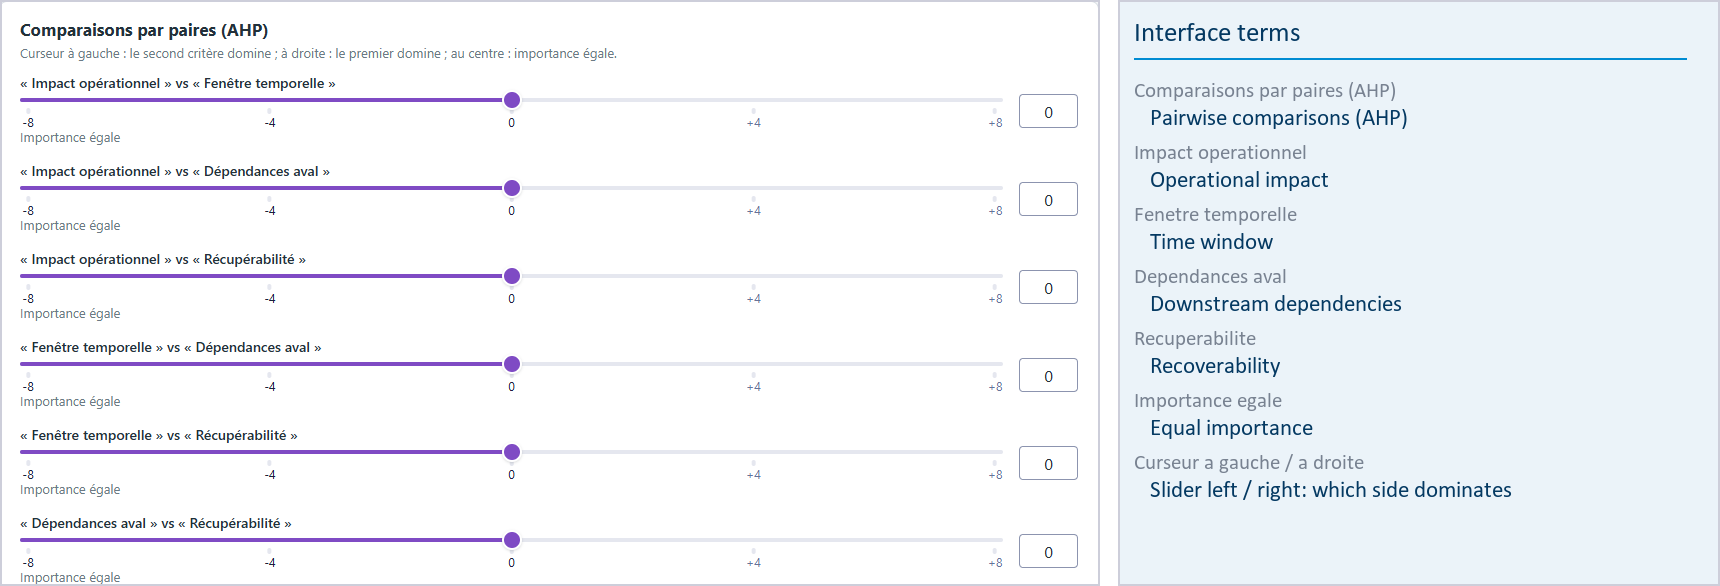
\includegraphics[width=\linewidth]{Images/4.Operations/questionnaire_annotated.png}
    \caption[The AHP questionnaire page]{The AHP questionnaire page, with its interface terms
    keyed into English. Six comparisons cover the four criteria.}
    \label{fig:questionnaire}
\end{figure}

\subsubsection*{Fuzzy BWM and PROMETHEE II Network Outranking}
\label{sec:fbwm_promethee}

The modules \texttt{mcda/fbwm.py} and \texttt{mcda/promethee.py} implement the two
complementary methods of Figure~\ref{fig:mcda_pipeline}: Fuzzy BWM offers a lower-effort
elicitation route than crisp AHP for weighting the six KPI blocks, and PROMETHEE~II turns
those weights into a network-wide, non-compensatory ranking of nodes.

\paragraph{Fuzzy BWM.}
The elicitation cost is the reason the method is there. AHP needs $n(n-1)/2$ comparisons,
which is fifteen for the six blocks; the Best-Worst Method needs $2n-3$, which is nine, and
it obtains them by asking the operator to name only the most important block $B$ and the
least important block $W$ and then to judge $B$ against every other block and every other
block against $W$~\autocite{rezaei2015best}. The fuzzy variant replaces each judgement by a
triangular fuzzy number $(l, m, u)$ drawn from a five-point linguistic
scale~\autocite{guo2017fuzzy}, so that the operator's hesitation is carried through the
arithmetic instead of being rounded away at the door. Table~\ref{tab:fbwm_scale} gives the
scale as implemented.

\begin{table}[htbp]
\centering
\caption[The fuzzy linguistic scale]{The linguistic scale of the fuzzy Best-Worst Method, as
implemented in \texttt{mcda/fbwm.py}}
\label{tab:fbwm_scale}
\small
\begin{tabularx}{\linewidth}{@{}X l@{}}
\toprule
\textbf{Judgement} & \textbf{Triangular fuzzy number $(l,m,u)$} \\
\midrule
Equally important & $(1,\ 1,\ 1)$ \\
Weakly more important & $(2/3,\ 1,\ 3/2)$ \\
Moderately more important & $(3/2,\ 2,\ 5/2)$ \\
Very much more important & $(5/2,\ 3,\ 7/2)$ \\
Absolutely more important & $(7/2,\ 4,\ 9/2)$ \\
\bottomrule
\end{tabularx}
\end{table}

Writing $\tilde{a}_{Bj}$ for the fuzzy judgement of the best block against block $j$ and
$\tilde{a}_{jW}$ for that of block $j$ against the worst, the weights
$\tilde{w}_j = (l_j, m_j, u_j)$ solve the minimax programme
\begin{equation}
\begin{aligned}
    \min_{\tilde{w},\,\xi} \quad & \xi \\
    \text{s.t.} \quad
    & \bigl|\tilde{w}_B \oslash \tilde{w}_j - \tilde{a}_{Bj}\bigr| \le (\xi,\xi,\xi),
      && j \ne B, \\
    & \bigl|\tilde{w}_j \oslash \tilde{w}_W - \tilde{a}_{jW}\bigr| \le (\xi,\xi,\xi),
      && j \ne W, \\
    & \textstyle\sum_j R(\tilde{w}_j) = 1,
      \quad 0 < \epsilon \le l_j \le m_j \le u_j ,
\end{aligned}
\label{eq:fbwm}
\end{equation}
where the fuzzy quotient uses the standard interval approximation
$(l_1,m_1,u_1) \oslash (l_2,m_2,u_2) = (l_1/u_2,\, m_1/m_2,\, u_1/l_2)$ and $R$ is the
graded mean integration representation that defuzzifies a triangular number,
\begin{equation}
    R(l, m, u) = \frac{l + 4m + u}{6}.
    \label{eq:gmir}
\end{equation}
The objective $\xi$ is the largest deviation between any elicited judgement and the ratio the
solved weights actually imply, so it is a consistency measure of the same nature as the
$\mathrm{CR}$ above: a small $\xi$ says the operator's two comparison vectors are close to
being realisable by a single weight vector. The programme is non-linear and is solved by
sequential least squares from five seeded starting points, so a given questionnaire yields
the same weights on every run; if no start returns a feasible solution the module falls back
to uniform weights rather than raising, and the fallback is recorded. The output feeds
$\omega_m$ in Equation~\ref{eq:ur_local} and the criterion weights of PROMETHEE~II below, so
one elicitation serves both the per-node score and the network ranking.

\paragraph{PROMETHEE~II.}
Outranking answers a different question from scoring: not how urgent is this node, but which
node should be looked at before which other. For each ordered pair of nodes $(a,b)$ and each
criterion $j$, the oriented deviation $d_j(a,b) = g_j(a) - g_j(b)$ passes through a
preference function $P_j: \mathbb{R} \to [0,1]$, non-decreasing and null on $d \le 0$. The
six Brans-Vincke forms are implemented, usual, U-shape, V-shape, level, linear with
indifference, and Gaussian~\autocite{brans1986promethee}. The aggregated preference index and
the three flows are then
\begin{align}
    \pi(a,b) &= \sum_j w_j\, P_j\bigl(d_j(a,b)\bigr), \label{eq:promethee_pi} \\
    \phi^{+}(a) = \frac{1}{q-1}\sum_{b \ne a} \pi(a,b),
    \qquad
    \phi^{-}(a) &= \frac{1}{q-1}\sum_{b \ne a} \pi(b,a),
    \qquad
    \phi(a) = \phi^{+}(a) - \phi^{-}(a), \label{eq:promethee_flows}
\end{align}
over $q$ alternatives. The outgoing flow $\phi^{+}$ measures how far $a$ dominates the rest,
the incoming flow $\phi^{-}$ how far the rest dominates $a$, and the net flow $\phi$ gives a
complete ranking, which is what distinguishes PROMETHEE~II from the partial ranking of
PROMETHEE~I. The pairwise structure is where the $\Theta(k q^{2})$ term of
Table~\ref{tab:complexity} comes from.

Two properties of the implementation belong in the record. Missing data is handled per pair
rather than per node: for a pair and a criterion where either value is absent, $P_j$ is set
to zero in both directions and the weights are renormalised over the criteria present for
that pair alone, so a node with an incomplete KPI set is still ranked rather than dropped,
and if no criterion is present for a pair then $\pi(a,b) = \pi(b,a) = 0$. And PROMETHEE~II is
not independent of irrelevant alternatives: adding a node can invert the relative rank of two
existing nodes. That is a known and documented property of net-flow
methods~\autocite{triantaphyllou2000multi}, it is registered as a descriptive property-based test
rather than as a bug, and it is the reason the criticality index of
Section~\ref{sec:criticality} rather than the outranking is what hypothesis H3 is scored on.

\begin{figure}[htbp]
\centering
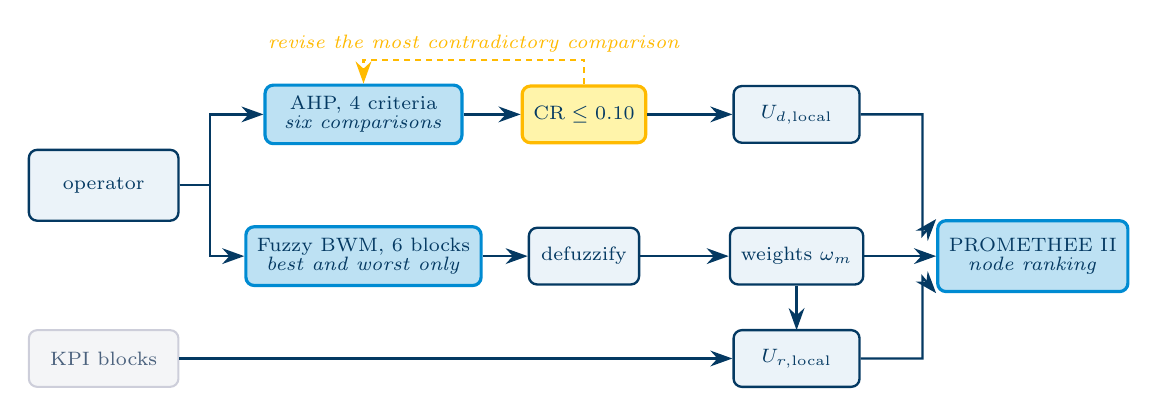
\begin{tikzpicture}[x=1cm, y=1cm, font=\scriptsize]

\node[bloc, minimum width=1.9cm, minimum height=0.9cm] (op) at (0.95, 0.55)
     {operator};

\node[blocFort, minimum width=2.5cm, minimum height=0.72cm] (ahp) at (4.25, 1.45)
     {AHP, 4 criteria\\[-1pt]\textit{six comparisons}};
\node[blocFort, minimum width=2.5cm, minimum height=0.72cm] (bwm) at (4.25, -0.35)
     {Fuzzy BWM, 6 blocks\\[-1pt]\textit{best and worst only}};

\node[blocAlerte, minimum width=1.4cm, minimum height=0.72cm] (gate) at (7.05, 1.45)
     {$\mathrm{CR} \le 0.10$};
\node[bloc, minimum width=1.4cm, minimum height=0.72cm] (gmir) at (7.05, -0.35)
     {defuzzify};

\node[bloc, minimum width=1.6cm, minimum height=0.72cm] (ud) at (9.75, 1.45)
     {$U_{d,\text{local}}$};
\node[bloc, minimum width=1.6cm, minimum height=0.72cm] (om) at (9.75, -0.35)
     {weights $\omega_m$};
\node[bloc, minimum width=1.6cm, minimum height=0.72cm] (ur) at (9.75, -1.65)
     {$U_{r,\text{local}}$};

\node[blocFort, minimum width=2.1cm, minimum height=0.9cm] (pro) at (12.75, -0.35)
     {PROMETHEE~II\\[-1pt]\textit{node ranking}};

\node[blocPale, minimum width=1.9cm, minimum height=0.72cm] (kpi) at (0.95, -1.65)
     {KPI blocks};

\draw[fleche] (op.east) -- (2.30, 0.55) -- (2.30, 1.45) -- (ahp.west);
\draw[fleche] (op.east) -- (2.30, 0.55) -- (2.30, -0.35) -- (bwm.west);
\draw[fleche] (ahp) -- (gate);
\draw[fleche] (bwm) -- (gmir);
\draw[fleche] (gate) -- (ud);
\draw[fleche] (gmir) -- (om);
\draw[fleche] (kpi.east) -- (ur.west);
\draw[fleche] (om.south) -- (9.75, -1.29);
\draw[fleche] (ur.east) -- (11.35, -1.65) -- (11.35, -0.62) -- (pro.south west);
\draw[fleche] (om.east) -- (pro.west);
\draw[fleche] (ud.east) -- (11.35, 1.45) -- (11.35, -0.08) -- (pro.north west);

\draw[flecheCoupee] (gate.north) -- (7.05, 2.15) -- (4.25, 2.15) -- (ahp.north);
\node[etiquette, anchor=south, text=altenOchreDark] at (5.65, 2.15)
     {revise the most contradictory comparison};

\end{tikzpicture}
\caption[The multi-criteria chain, from elicitation to ranking]{The two elicitation routes and
what they feed. AHP weights four declared criteria behind a consistency gate that returns an
incoherent questionnaire to the operator; Fuzzy BWM weights the six KPI blocks, and those same
weights $\omega_m$ serve both the noisy-OR aggregation and the PROMETHEE~II criteria, so the
network ranking and the per-node score stay mutually consistent rather than resting on a
separately calibrated weight set.}
\label{fig:mcda_pipeline}
\end{figure}

The linguistic scale maps five qualitative judgements to triangular fuzzy numbers on a
1 to 4.5 scale, each carrying its own maximum consistency index. The consistency ratio is
$\mathrm{CR}_{\text{BWM}} = \xi^*/\mathrm{CI}$, where $\xi^*$ is the optimal consistency
indicator returned by a constrained non-linear optimisation fitting the fuzzy weights to
the elicited comparisons. If the optimisation fails to converge, the implementation falls
back to uniform weights rather than raising an error, so a single malformed elicitation
cannot break the weekly review. Fuzzy weights are defuzzified with the Graded Mean
Integration Representation,

\begin{equation}
    w_j = \frac{a_j + 4 b_j + c_j}{6},
    \label{eq:bwm_defuzz}
\end{equation}

then renormalised to sum to one. The triangular bounds are written $(a_j, b_j, c_j)$ rather
than the more common $(l_j, m_j, u_j)$ to avoid colliding with the risk blocks $u_m$.

PROMETHEE~II ranks the active nodes of a project on the same six weighted urgency blocks
that feed local real urgency. For each pair of active nodes and each block, the preference
intensity is computed with a Type~V linear preference function with an indifference
threshold, and the aggregated preference index and net outranking flow follow the standard
formulation:

\begin{equation}
    \pi(a,b) = \sum_m \omega_m P_m\bigl(g_m(a) - g_m(b)\bigr), \qquad
    \phi(a) = \phi^+(a) - \phi^-(a).
    \label{eq:promethee_net}
\end{equation}



\subsection{The forecast layer, specified}
\label{sec:methods_forecast}

The results of this thesis turn on one component, so it is specified here rather than left
implicit behind the phrase used in the scoring protocol below. The forecast service projects
every active node over one to four weeks from that node's own persisted weekly history, and
emits the probability $p_h$ that an adverse outcome occurs within the horizon.

Three quantities are estimated from the node's own weekly history and then simulated
forward, and $p_h$ is the fraction of trajectories in which the outcome occurs. Each is
given here in full, because the results of Section~\ref{sec:Results} are results about this
estimator and about nothing else.

\paragraph{The urgency path.}
Local real urgency is modelled as a mean-reverting first-order autoregression on the weekly
series $x_1, \ldots, x_T$ of that node,
\begin{equation}
    x_{k} = \mu + \varphi\,(x_{k-1} - \mu) + \sigma\,\varepsilon_k,
    \qquad \varepsilon_k \sim \mathcal{N}(0,1),
    \label{eq:ar1}
\end{equation}
with $\mu$ the sample mean of the series. The coefficient $\varphi$ is the ordinary
least-squares slope of $x_{t+1}$ on $x_t$ and $\sigma$ the residual standard deviation,
\begin{equation}
    \varphi = \frac{\sum_t (x_t - \bar{x})(x_{t+1} - \bar{z})}{\sum_t (x_t - \bar{x})^2},
    \qquad
    \sigma^2 = \frac{1}{T-2}\sum_t \hat{\varepsilon}_t^{\,2},
    \label{eq:ar1_fit}
\end{equation}
with the standard errors that the outer draw below consumes,
$\mathrm{se}(\varphi) = \sigma / \sqrt{S_{xx}}$ where $S_{xx} = \sum_t (x_t-\bar{x})^2$, and
$\mathrm{se}(\sigma) = \sigma / \sqrt{2(T-2)}$.

Three guards apply, and each is a modelling decision rather than a numerical convenience.
The slope is clipped to $[0, 0.98]$: the upper bound keeps the process strictly stationary,
so a projection cannot diverge over four weeks, and the lower bound at zero forbids negative
autocorrelation, which on an urgency series would mean a node alternating between calm and
crisis every week for no physical reason. The residual scale is floored at $0.01$ before the
standard errors are computed, so a node whose history happens to be flat still carries some
forward uncertainty rather than announcing its current state with certainty. And a
degenerate series, one with $S_{xx}$ at machine zero, falls back to $\varphi = 0$ with
residuals taken about the mean, which is the honest reading that the history contains no
usable dynamics.

\paragraph{The event rate.}
Each week of history is a Bernoulli trial, a success being a week in which at least one
non-reverted event of gravity critical or defect is logged, the same gravities the
calibration service uses. With $k$ successes in $T$ weeks the rate $\tau$ has the conjugate
Beta posterior
\begin{equation}
    \tau \mid k, T \;\sim\; \mathrm{Beta}\bigl(\alpha_0 + k,\; \beta_0 + T - k\bigr),
    \qquad
    \alpha_0 = \tau_0 N_0, \quad \beta_0 = (1-\tau_0) N_0,
    \label{eq:beta_posterior}
\end{equation}
with a prior of mean $\tau_0 = 0.03$ and strength $N_0 = 26$ pseudo-observations, so
$\alpha_0 = 0.78$ and $\beta_0 = 25.22$. The strength is the repository convention of half a
year of weekly observations, and it is deliberately heavy relative to the campaign: with
nineteen turns of history at most, the prior still carries more weight than the data, so an
early node with one bad week is not immediately declared high-risk. That is a conservative
choice in one direction and a sluggish one in the other, and Section~\ref{sec:res_mechanism}
reports which of the two the campaign actually paid for.

\paragraph{The lead-time law.}
The moments of the lead-time distribution are drawn through a parametric bootstrap on the
same $N_0 = 26$ pseudo-observation convention, so their uncertainty shrinks as
$1/\sqrt{N_0}$ rather than being treated as known exactly.

\paragraph{The nested draw, and what the interval covers.}
These three sources are parameters, not observations, so simulating trajectories at their
point estimates would report only the sampling noise of the simulator and would call a
forecast precise whenever the simulator was cheap. The rollout therefore nests two loops:
$K = 20$ outer draws of the parameters themselves, each carrying $S = n/K$ inner
trajectories, for $n$ trajectories in total. Writing $\hat{p}_k$ for the outcome frequency
within outer draw $k$, the estimator and its two variance components are
\begin{equation}
    \hat{p} = \frac{1}{K}\sum_{k=1}^{K} \hat{p}_k,
    \qquad
    \widehat{V}_{\mathrm{mc}} = \frac{1}{K}\sum_{k=1}^{K} \hat{p}_k(1-\hat{p}_k),
    \qquad
    \widehat{V}_{\mathrm{par}} = \frac{1}{K-1}\sum_{k=1}^{K} (\hat{p}_k - \hat{p})^2 .
    \label{eq:variance_components}
\end{equation}
This is the law of total variance applied to the parameter vector $\theta$,
\begin{equation}
    \operatorname{Var}(\hat{p})
    = \underbrace{\mathbb{E}_{\theta}\bigl[\operatorname{Var}(\hat{p} \mid \theta)\bigr]}
      _{\text{Monte Carlo, within a draw}}
    + \underbrace{\operatorname{Var}_{\theta}\bigl[\mathbb{E}(\hat{p} \mid \theta)\bigr]}
      _{\text{parametric, between draws}} ,
    \label{eq:total_variance}
\end{equation}
and it is what the two braces of Figure~\ref{fig:forecast_rollout} denote. The first
component is reducible by simulating more trajectories; the second is not, and shrinks only
with more weeks of history.

The reported interval combines them asymmetrically, and the asymmetry is deliberate:
\begin{equation}
    \mathrm{se}_{\mathrm{mc}} = \sqrt{\widehat{V}_{\mathrm{mc}} / n},
    \qquad
    \mathrm{se}_{\mathrm{tot}} = \sqrt{\widehat{V}_{\mathrm{par}}
                                       + \widehat{V}_{\mathrm{mc}} / n},
    \qquad
    \mathrm{IC}_{80} = \hat{p} \pm 1.2816\,\mathrm{se}_{\mathrm{tot}},
    \label{eq:ic80}
\end{equation}
clipped to $[0,1]$ and tagged in the data model with the coverage it claims. The Monte Carlo
term enters divided by $n$, because it is the standard error of an estimator and shrinks with
the simulation budget. The parametric term enters undivided, and that is the point: the
quantity of interest is $p$ itself and not $\mathbb{E}[p]$, so the parametric spread is a
dispersion the forecast genuinely has rather than an estimation error the reader could
average away. An interval built the other way would narrow as $1/\sqrt{K}$ and would report
a confident forecast whenever twenty draws happened to be requested. The campaign runs at
$n = 500$, so $K = 20$ outer draws carry $S = 25$ trajectories each.

\paragraph{What this component is not.}
A second and separate path exists in the codebase, a frozen product model that standardises a
feature vector, scores it through a logistic regression and passes the result through an
isotonic calibrator. It consumes the rollout probability above as one of its input features.
It is named here only so that the boundary is unambiguous: it is not the component scored
anywhere in this thesis, and every figure in Section~\ref{sec:Results} comes from the nested
rollout of Equation~\ref{eq:variance_components}, at five hundred trajectories, as the
recorded forecast logs confirm.


The estimator is deliberately tied to the target. What $p_h$ estimates is exactly the adverse
outcome of the calibration service, a missed milestone or a non-reverted event of gravity
critical or defect; the third condition of that definition, node abandonment, is not
simulated, because only active nodes are projected and abandonment is an outcome to
anticipate rather than an input state. The forecast is therefore the prospective estimator of
the quantity the calibration service measures retrospectively. Section~\ref{sec:res_target_trap}
shows how much rests on that alignment.

Uncertainty is decomposed rather than lumped, through the nested draw of
Figure~\ref{fig:forecast_rollout}: the variance of $p_h$ splits into a Monte Carlo component
within outer draws and a parametric component between them, and the reported interval is
labelled by the sources it covers. This matters for the reliability analysis of
Section~\ref{sec:res_armA_scored}, since an interval that hides which uncertainty it
represents cannot be read.

\begin{figure}[htbp]
\centering
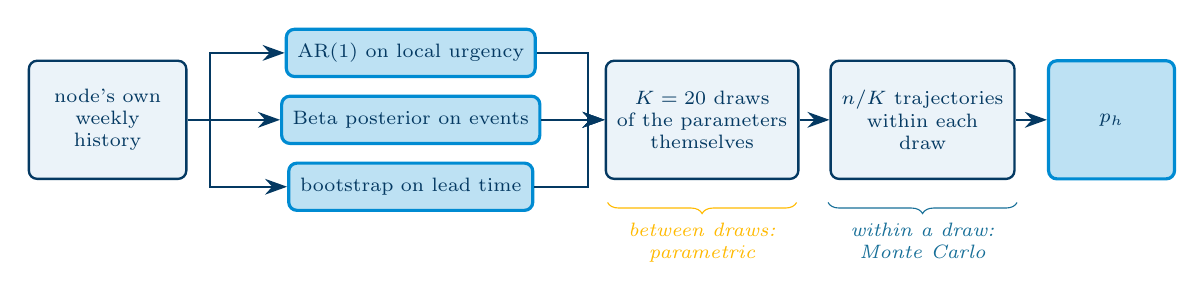
\begin{tikzpicture}[x=1cm, y=1cm, font=\scriptsize]

\node[bloc, minimum width=2.0cm, minimum height=1.5cm] (hist) at (1.0, 0)
     {node's own\\weekly\\history};

\node[blocFort, minimum width=3.1cm, minimum height=0.6cm] (ar)  at (4.85, 0.85)
     {AR(1) on local urgency};
\node[blocFort, minimum width=3.1cm, minimum height=0.6cm] (bet) at (4.85, 0.0)
     {Beta posterior on events};
\node[blocFort, minimum width=3.1cm, minimum height=0.6cm] (boo) at (4.85, -0.85)
     {bootstrap on lead time};

\node[bloc, minimum width=2.3cm, minimum height=1.5cm] (outer) at (8.55, 0)
     {$K = 20$ draws\\of the parameters\\themselves};
\node[bloc, minimum width=2.3cm, minimum height=1.5cm] (inner) at (11.35, 0)
     {$n/K$ trajectories\\within each\\draw};
\node[blocFort, minimum width=1.6cm, minimum height=1.5cm] (ph) at (13.75, 0) {$p_h$};

\draw[fleche] (hist.east) -- (2.3, 0) -- (2.3, 0.85) -- (ar.west);
\draw[fleche] (hist.east) -- (bet.west);
\draw[fleche] (hist.east) -- (2.3, 0) -- (2.3, -0.85) -- (boo.west);
\draw[fleche] (ar.east) -- (7.1, 0.85) -- (7.1, 0) -- (outer.west);
\draw[fleche] (bet.east) -- (outer.west);
\draw[fleche] (boo.east) -- (7.1, -0.85) -- (7.1, 0) -- (outer.west);
\draw[fleche] (outer) -- (inner);
\draw[fleche] (inner) -- (ph);

\draw[decorate, decoration={brace, amplitude=4pt, mirror}, draw=altenOchreDark]
     (7.35, -1.05) -- (9.75, -1.05);
\node[etiquette, anchor=north, text=altenOchreDark] at (8.55, -1.22)
     {between draws:\\parametric};
\draw[decorate, decoration={brace, amplitude=4pt, mirror}, draw=altenAzureDark]
     (10.15, -1.05) -- (12.55, -1.05);
\node[etiquette, anchor=north, text=altenAzureDark] at (11.35, -1.22)
     {within a draw:\\Monte Carlo};

\end{tikzpicture}
\caption[The nested forecast rollout]{The nested rollout. Three quantities are estimated from
the node's own history, then drawn $K$ times through their own uncertainty, the
autoregression coefficient and residual scale through their least-squares standard errors,
the event rate through its Beta posterior, the lead-time moments through the bootstrap,
and each draw carries its own trajectories. The two braces are the two variance components
the reported interval distinguishes.}
\label{fig:forecast_rollout}
\end{figure}

Two disciplines are enforced in the code rather than by convention. The service never writes,
so a forecast cannot perturb the state it forecasts. And counterfactual comparisons, which
price a corrective action by rerunning two branches on common random numbers, are named
throughout as an effect according to the model and never as a measured effect, because both
branches are simulated and neither is an observation.



\subsection{Computational complexity and measured scalability}
\label{sec:complexity}

The campaign graphs are small, eight nodes on the first chain and fifteen on the second, so
nothing in the results depends on performance. The question this subsection answers is a
different one: whether the design would survive a real programme, where a tier-one supply
network runs to hundreds or thousands of nodes. Two things are needed for that, a complexity
that does not grow faster than the graph and a measurement confirming the constant is small.

Table~\ref{tab:complexity} gives the first. Every entry follows from
Proposition~\ref{prop:propagation}(iv), since each operation is a fixed number of topological
passes over the graph, and the only quadratic term in the system is the pairwise outranking of
PROMETHEE~II, which runs over criteria and alternatives rather than over the network.

\begin{table}[htbp]
\centering
\caption[Complexity of the principal operations]{Complexity of the principal operations, in a
graph of $n$ nodes and $e$ arcs}
\label{tab:complexity}
\small
\begin{tabularx}{\linewidth}{@{}l l X@{}}
\toprule
\textbf{Operation} & \textbf{Time} & \textbf{Remark} \\
\midrule
Topological order & $\Theta(n + e)$ & Kahn; nominal arcs only \\
Full propagation, $U_d$ and $U_r$ & $\Theta(n + e)$ & Two passes, one per direction \\
Incremental propagation & $\Theta(|C| + |E(C)|)$ & Restricted to the affected cone $C$ \\
Log-survival twin & $\Theta(n + e)$ & One logarithm per node and per arc \\
Local urgency, six blocks & $\Theta(1)$ per node & Fixed number of KPI terms \\
Adequacy score & $\Theta(1)$ per node & Closed form, Equation~\ref{eq:At} \\
Monte Carlo lead time & $\Theta(N(n+e))$ & $\Theta(Nn)$ space, guarded at $5\times10^{7}$ \\
Criticality index & $\Theta(n_{\text{act}}(n+e))$ & Doubled by the twin; no incremental form \\
Probabilistic criticality & $\Theta(S(n+e))$ per node & Vectorised over the $S$ draws \\
PROMETHEE~II outranking & $\Theta(k\,q^{2})$ & $q$ alternatives on $k$ criteria \\
\bottomrule
\end{tabularx}
\end{table}

Table~\ref{tab:benchmarks} gives the second. The figures are wall-clock means from the
benchmark suite, run on a reproducible stress graph of $1\,000$ nodes and $1\,244$ arcs over
twenty-five ranks, generated from a fixed seed so that successive runs measure the same work.
The machine is the development laptop described in Section~\ref{sec:methods_repro}, an AMD
Ryzen~7~PRO~8840HS with sixteen threads and $11.7$~GB of memory, under CPython~3.12.1, with no
GPU involved at any point. Each row reports the mean over the number of rounds the harness
chose, together with its standard deviation.

\begin{table}[htbp]
\centering
\caption[Measured performance at one thousand nodes]{Measured performance on a $1\,000$-node,
$1\,244$-arc stress graph}
\label{tab:benchmarks}
\small
\begin{tabularx}{\linewidth}{@{}X r r r@{}}
\toprule
\textbf{Operation} & \textbf{Mean (ms)} & \textbf{SD (ms)} & \textbf{Rounds} \\
\midrule
Incremental propagation, one node changed & $1.04$ & $0.25$ & $472$ \\
What-if shock on a rank-25 supplier & $4.99$ & $1.06$ & $224$ \\
Full propagation, $U_d$ and $U_r$ & $6.34$ & $1.12$ & $129$ \\
Dashboard network figure & $43.7$ & $1.0$ & $5$ \\
Evaluate every node and persist & $105.2$ & $16.2$ & $3$ \\
Monte Carlo lead time, $N = 10\,000$ & $478.8$ & $33.9$ & $3$ \\
Load the graph from the registry & $782.1$ & $39.8$ & $3$ \\
\bottomrule
\end{tabularx}
\end{table}

\begin{figure}[htbp]
    \centering
    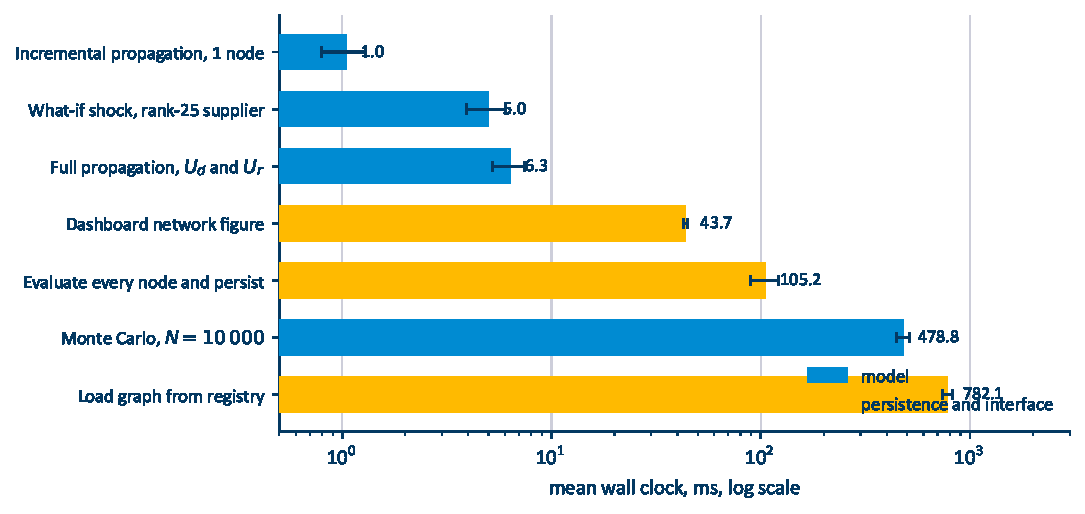
\includegraphics[width=0.92\linewidth]{Images/benchmarks.pdf}
    \caption[Measured performance at one thousand nodes]{The same seven operations on a log
    scale, model work in azure and persistence or interface work in ochre. Three orders of
    magnitude separate an incremental propagation from a graph load, and the operations a user
    waits on repeatedly are the fast ones.}
    \label{fig:benchmarks}
\end{figure}

Three readings matter. A full propagation of a thousand-node network costs $6.3$~ms, so the
recomputation triggered by a weekly review is imperceptible and the interactive what-if of
Section~\ref{sec:methods_impl} is genuinely interactive rather than nominally so. The
incremental pass is $6.1$ times faster than the full one, which is the empirical form of
Proposition~\ref{prop:propagation}(iii): the cone of a single changed node is a small
fraction of the graph, and everything outside it is read from cache without approximation.
And the Monte Carlo layer at $479$~ms is two orders of magnitude above the analytic path,
which is why it is an opt-in per project rather than the default, and why the memory guard
exists at all: at ten thousand draws over a thousand nodes the simulation holds
$10^{7}$ completion times in memory at once.

The one operation that dominates is loading the graph from the registry at $782$~ms, and it
is a persistence cost rather than a model cost. It is paid once per session, not per
recomputation, which is the reason it was left alone: optimising it would improve a number
nobody waits on twice.

%% ═══════════════════════════════════════════════════════════════════════════


%% ═══════════════════════════════════════════════════════════════════════════
\section{Observed Capacity: An Opening}
\label{app:opening}
%% ═══════════════════════════════════════════════════════════════════════════

Section~\ref{sec:limitations} records that the satellite work is reported as an
opening and claimed as no part of the contribution: nothing joins it to the
urgency model. It is set out here for that reason, with its protocol and data in
Appendix~\ref{app:volume}.

\label{sec:res_volume}
%% ═══════════════════════════════════════════════════════════════════════════

Every KPI reaching the six blocks arrives either through a manual weekly review or through a
scripted event, so a node's score is never fresher than its last submitted review, and the
capacity block in particular depends on the same operator whose declaration the adequacy
score exists to audit. The independence that Section~\ref{sec:res_discussion} identifies as
the precondition for the whole measurement is therefore not structurally guaranteed.

A second system, developed alongside the main work, addresses one part of that dependency by
estimating the physical capacity of a warehouse from public satellite imagery, which is an
observation no operator supplies and none can bias. It is an opening rather than a second
contribution: the two systems have not been connected, and no claim is made that they have.
The pipeline takes a coordinate, retrieves the building footprint from the French national
topographic database, retrieves 20~cm orthophotography and, where available, a LiDAR surface
model, and derives a storable volume as $0.80 \times \text{footprint} \times \text{height}$
and a transfer capacity as the equipped facade length divided by a dock pitch of $3.8$~m.
Both constants are calibrated rather than assumed, and Appendix~\ref{app:volume} gives each
with the sample behind it, together with the one that does not survive audit: the fill factor
of $0.80$ is attributed in the source to a 122-site calibration whose detailed output was not
retained, and recomputing it over the 68 sites still on disk gives a median of $0.97$. The
volumetric figures below carry that unquantified bias; the dock figures, which depend on the
pitch instead, do not.

\subsection{The Physical Limit and the Reframing}
\label{sec:res_volume_limit}

The original objective was to count loading docks. That objective is unreachable, and
establishing why is the most transferable result of this work.

An empty dock door under a canopy produces no measurable signal from directly overhead.
Measured contrast at verified empty bays is $0.18\sigma$, $0.22\sigma$ and $0.01\sigma$
across a full sweep of assumed depths, while occupied bays on the same facades register at
$5.3\sigma$ to $6.4\sigma$. The measurement is sensitive enough; the signal is absent.
Repeating the test on 8~cm very-high-resolution imagery leaves the doors equally invisible,
which shows the cause to be occlusion by the canopy roof rather than insufficient resolution.
A gain of $2.5\times$ in ground sample distance recovers no additional door: what improves
with resolution is everything except the quantity of interest. Any method claiming to count
empty doors one by one from a nadir view is recovering an artefact.

That finding splits the problem in two. Counting each door individually is not observable at
nadir, and no amount of resolution changes it. Recognising that a facade is equipped for
docking, and delimiting its extent, is observable, because the canopy, the apron and the bay
rhythm remain visible whether or not a vehicle is present. The second formulation is
learnable, and it is sufficient, because capacity is a function of equipped length rather
than of individually identified doors. Figure~\ref{fig:volume_proof} is the direct evidence:
three facades of 135~m, 105~m and 15~m on which the automatic trailer detector found no
vehicle at all, where individual doors are not resolvable and the bay markings and canopy
edge are.

\begin{figure}[htbp]
    \centering
    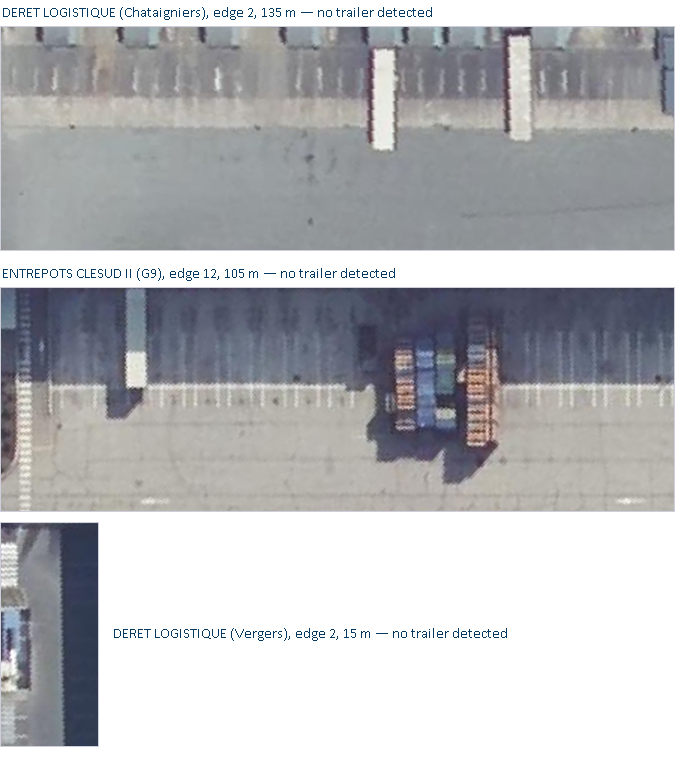
\includegraphics[width=0.72\linewidth, height=0.42\textheight, keepaspectratio]{Images/5.Volume/facade_proof_en.png}
    \caption{Equipped facades on which no trailer was detected}
    \label{fig:volume_proof}
\end{figure}

One reservation is recorded honestly. The proportion of sites showing no usable dock
signature was measured on a subsample that required vehicles to be present to establish
ground truth, and is therefore biased towards sites with vehicles. Five zero-shot approaches
were tried before the reframing and each was abandoned for a measured reason;
Appendix~\ref{app:volume} records them, because the reasons constrain what a successful
method can look like.

\subsection{Learned Dock-Zone Segmentation}
\label{sec:res_volume_seg}

The reframed problem was addressed by training a segmentation model to delimit equipped
facade zones directly. Table~\ref{tab:volume_training} gives the progression across four
training runs, read at the best epoch of each by mask mAP50-95.

\begin{table}[htbp]
\centering
\caption{Segmentation training progression}
\label{tab:volume_training}
\small
\begin{tabularx}{\linewidth}{l >{\centering\arraybackslash}X >{\centering\arraybackslash}X >{\centering\arraybackslash}X >{\centering\arraybackslash}X >{\centering\arraybackslash}X >{\centering\arraybackslash}X}
\toprule
\textbf{Run} & \textbf{Train / val} & \textbf{Image size} & \textbf{Precision} &
\textbf{Recall} & \textbf{mAP50} & \textbf{mAP50-95} \\
\midrule
1 & 86 & 640 & 0.461 & 0.404 & 0.363 & 0.155 \\
2 & 203 / 50 & 640 & 0.635 & 0.539 & 0.610 & 0.283 \\
3 & 351 / 91 & 640 & \textbf{0.702} & \textbf{0.606} & \textbf{0.618} & \textbf{0.305} \\
4 & 351 / 91 & 1280 & 0.652 & 0.547 & 0.570 & 0.272 \\
\bottomrule
\end{tabularx}
\end{table}

\begin{figure}[htbp]
    \centering
    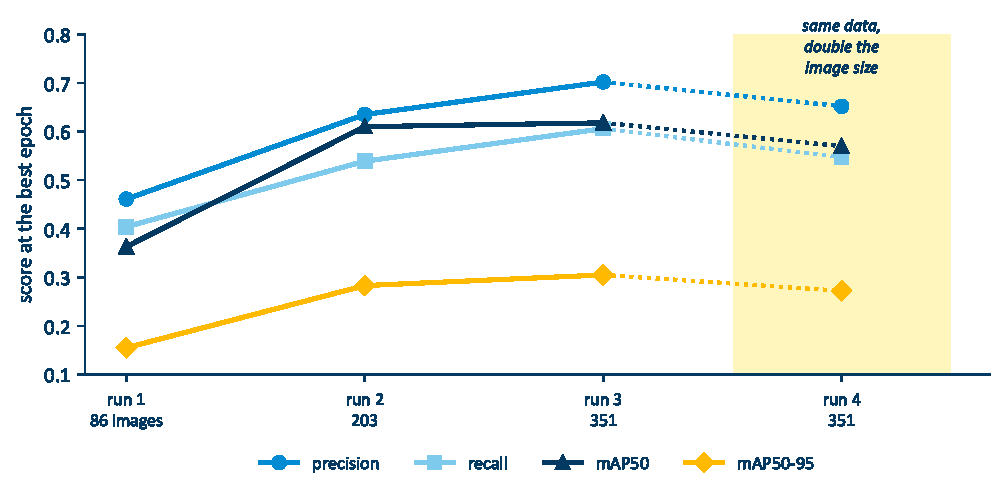
\includegraphics[width=0.94\linewidth]{Images/segmentation_runs.pdf}
    \caption[What moved the segmentation model]{The same four runs plotted. Runs~1 to~3 raise
    the training set at a fixed image size and every metric rises with it. Run~4 holds the set
    and doubles the image size instead, and every metric falls. The binding constraint was
    annotated data rather than resolution, which is a conclusion about the corpus and not
    about the architecture.}
    \label{fig:segmentation_runs}
\end{figure}

Figure~\ref{fig:segmentation_runs} makes the cause visible: quadrupling the training set from 86 to 351 images roughly
doubled mask mAP50-95. Resolution did not: run 4 is identical to run 3 except for a doubled
input size, and it is worse on every metric, so at a fixed data budget and a CPU-only
training budget the additional pixels cost more than they bought.

What is measured matters as much as the score. Standard detection metrics score shape
overlap, but the operational quantity is capacity, which depends only on the length of the
equipped zone: a polygon drawn too deep, or with imprecise edges, still yields the correct
dock count. The project therefore scores itself on the error in the derived dock count rather
than on mAP, and that business metric is the one used to decide whether a model is good
enough to deploy. On the reference run it reports a global bias of $-35\%$, a median error of
$62\%$ on images containing docks, and $89\%$ of true negatives correctly left empty, which
is a system that is directionally useful and quantitatively not yet trustworthy.

The pipeline runs end to end on a geographic area, retrieving footprints, presenting each to
the trained model, assigning predicted zones to the correct building and writing capacity
figures. One defect found during that deployment is recorded in Appendix~\ref{app:volume}
because it illustrates the difference between a model error and a systems error, as is the
annotation episode in which an automated third-party process reported 442 annotations as
verified and complete while having placed a zone along every edge of every building without
examining the imagery at all.

\subsection{What This Can and Cannot Feed}
\label{sec:res_volume_bridge}

The system supplies a storable volume, a pallet-position estimate and, where a dock zone is
detected, a transfer capacity and an occupancy ratio. Those map onto the capacity block of
Equation~\ref{eq:ur_local} and onto nothing else: it says nothing about lead time, cost or
emissions. Coverage is metropolitan France, bounded by the public data services it draws on.
The trained segmentation model is not yet wired into the production capacity path, which
still uses the zero-shot trailer method and its $36\%$ coverage. And the imagery is a
snapshot, so the resulting figure is a structural capacity rather than a live occupancy.

What it does change is the provenance of one input. A capacity figure derived from imagery is
not supplied by the operator whose declaration the adequacy score audits, which is precisely
the independence Section~\ref{sec:res_discussion} identifies as the precondition for the
measurement to mean anything. Figure~\ref{fig:volume_bridge} states where that input would
enter and, equally important, which blocks it would leave untouched.

\begin{figure}[htbp]
\centering
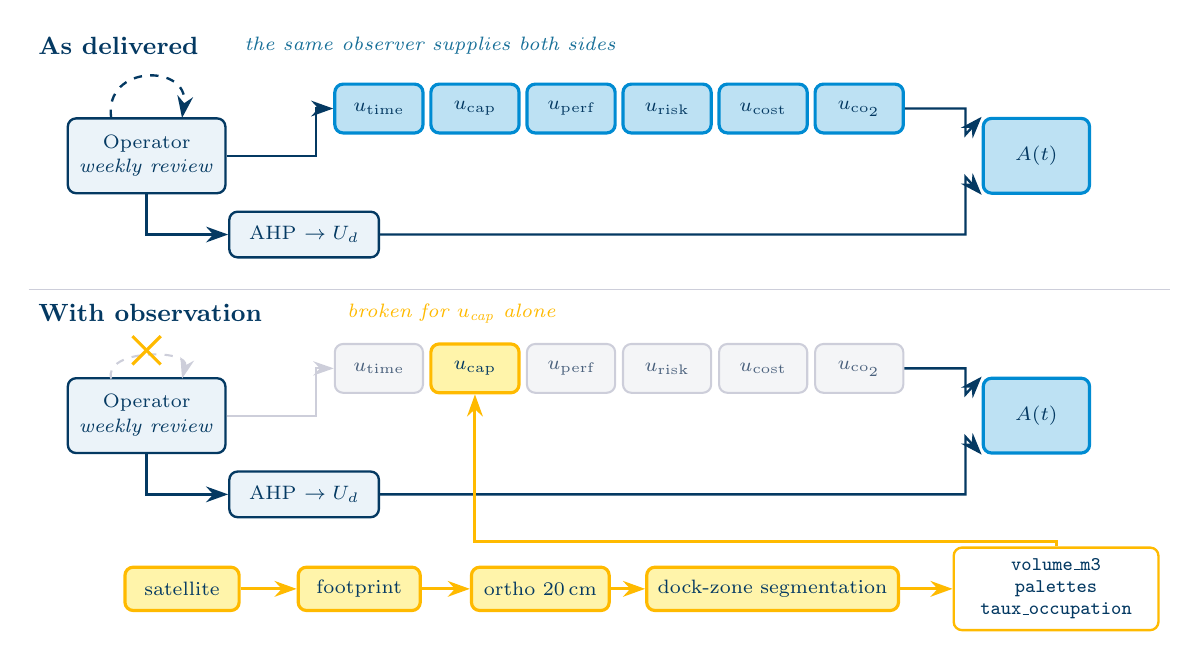
\begin{tikzpicture}[x=1cm, y=1cm, font=\scriptsize]

%% ── Bande haute : le systeme tel qu'il est livre ────────────────────────────
\node[titreBande, anchor=west] at (-0.9, 1.95) {As delivered};
\node[etiquette, anchor=west] at (1.75, 1.95) {the same observer supplies both sides};

\node[bloc, minimum width=2.0cm, minimum height=0.95cm] (opA) at (0.6, 0.55)
     {Operator\\[1pt]\textit{weekly review}};

\foreach \i/\lab in {0/{$u_{\text{time}}$}, 1/{$u_{\text{cap}}$}, 2/{$u_{\text{perf}}$},
                     3/{$u_{\text{risk}}$}, 4/{$u_{\text{cost}}$}, 5/{$u_{\text{co}_2}$}}
  \node[blocFort, minimum width=1.12cm, minimum height=0.62cm]
       (tA\i) at (3.55 + 1.22*\i, 1.15) {\lab};

\node[bloc, minimum width=1.9cm, minimum height=0.58cm] (ahpA) at (2.60, -0.45)
     {AHP $\rightarrow U_d$};

\node[blocFort, minimum width=1.35cm, minimum height=0.95cm] (adqA) at (11.9, 0.55)
     {$A(t)$};

\draw[fleche] (opA.east) -- (2.75, 0.55) -- (2.75, 1.15) -- (tA0.west);
\draw[fleche] (opA.south) |- (ahpA.west);
\draw[fleche] (tA5.east) -- (11.0, 1.15) -- (11.0, 0.82) -- (adqA.north west);
\draw[fleche] (ahpA.east) -- (11.0, -0.45) -- (11.0, 0.28) -- (adqA.south west);

\draw[fleche, dashed] (0.15, 1.03) .. controls (0.05, 1.72) and (1.15, 1.72) .. (1.05, 1.03);

\draw[altenGreyLine, line width=0.6pt] (-0.9, -1.15) -- (13.6, -1.15);

%% ── Bande basse : avec le canal observe ─────────────────────────────────────
\node[titreBande, anchor=west] at (-0.9, -1.45) {With observation};

\node[etiquette, anchor=west, text=altenOchreDark] at (3.05, -1.45)
     {broken for $u_{\text{cap}}$ alone};

\node[bloc, minimum width=2.0cm, minimum height=0.95cm] (opB) at (0.6, -2.75)
     {Operator\\[1pt]\textit{weekly review}};

\foreach \i/\lab in {0/{$u_{\text{time}}$}, 2/{$u_{\text{perf}}$}, 3/{$u_{\text{risk}}$},
                     4/{$u_{\text{cost}}$}, 5/{$u_{\text{co}_2}$}}
  \node[blocPale, minimum width=1.12cm, minimum height=0.62cm]
       (tB\i) at (3.55 + 1.22*\i, -2.15) {\lab};
\node[blocObs, minimum width=1.12cm, minimum height=0.62cm]
     (tB1) at (4.77, -2.15) {$u_{\text{cap}}$};

\node[bloc, minimum width=1.9cm, minimum height=0.58cm] (ahpB) at (2.60, -3.75)
     {AHP $\rightarrow U_d$};

\node[blocFort, minimum width=1.35cm, minimum height=0.95cm] (adqB) at (11.9, -2.75)
     {$A(t)$};

\draw[flechePale] (opB.east) -- (2.75, -2.75) -- (2.75, -2.15) -- (tB0.west);
\draw[fleche] (opB.south) |- (ahpB.west);
\draw[fleche] (tB5.east) -- (11.0, -2.15) -- (11.0, -2.48) -- (adqB.north west);
\draw[fleche] (ahpB.east) -- (11.0, -3.75) -- (11.0, -3.02) -- (adqB.south west);

%% la meme boucle qu'au-dessus, au meme endroit, mais rompue
\draw[flechePale, dashed] (0.15, -2.28) .. controls (0.05, -1.90) and (1.15, -1.90) ..
     (1.05, -2.28);
\draw[altenOchreDark, line width=1.1pt] (0.42, -2.10) -- (0.78, -1.74);
\draw[altenOchreDark, line width=1.1pt] (0.42, -1.74) -- (0.78, -2.10);

%% le canal observe, qui n'atteint qu'un bloc
\node[blocObs, minimum width=1.45cm, minimum height=0.55cm] (sat) at (1.05, -4.95)
     {satellite};
\node[blocObs, minimum width=1.55cm, minimum height=0.55cm] (bdt) at (3.30, -4.95)
     {footprint};
\node[blocObs, minimum width=1.75cm, minimum height=0.55cm] (ort) at (5.60, -4.95)
     {ortho 20\,cm};
\node[blocObs, minimum width=2.60cm, minimum height=0.55cm] (seg) at (8.55, -4.95)
     {dock-zone segmentation};
\node[bloc, minimum width=2.60cm, minimum height=0.95cm, draw=altenOchreDark,
      fill=white] (sorties) at (12.15, -4.95)
     {\texttt{volume\_m3}\\\texttt{palettes}\\\texttt{taux\_occupation}};

\draw[flecheObs] (sat) -- (bdt);
\draw[flecheObs] (bdt) -- (ort);
\draw[flecheObs] (ort) -- (seg);
\draw[flecheObs] (seg) -- (sorties);
\draw[flecheObs] (sorties.north) -- (12.15, -4.35) -- (4.77, -4.35) -- (tB1.south);

\end{tikzpicture}
\caption[Where observed capacity would enter the real-urgency model]{Where
satellite-observed capacity would enter the real-urgency model, and which blocks it does not
reach. Above, every block and the declaration itself originate with the same observer, which
is the circularity of Section~\ref{sec:res_discussion}. Below, one block of six is fed by an
observation no operator supplies, so the circular dependency is cut for that block; the other
five, greyed, still arrive through the weekly review.}
\label{fig:volume_bridge}
\end{figure}


\subsection{Reference tables}

The tables below define the terms of the model equations, list the campaign's network
and events, and record the two literature comparisons. Each is referred to from the
body at the point it applies.

\begin{table}[htbp]
\centering
\caption{DISCO technology stack}
\label{tab:disco_stack}
\begin{tabularx}{\linewidth}{lX}
\toprule
\textbf{Component} & \textbf{Technology / Value} \\
\midrule
Backend API    & Spring Boot + Java~21 \\
Database       & PostgreSQL (Azure) \\
Frontend       & Angular \\
Authentication & Player key / Azure AD SSO OAuth2 \\
Scores computed & CO\textsubscript{2}, Cost, Risk per supplier and itinerary, on $[1,10]$ \\
\bottomrule
\end{tabularx}
\end{table}

\begin{table}[htbp]
\centering
\caption[Aggregation and growth models found in the literature]{Aggregation and growth
models found in the literature. Figure~\ref{fig:aggregation_families} plots what each
one does.}
\label{tab:urgency_models}
\small
\begin{tabularx}{\linewidth}{>{\raggedright\arraybackslash}p{3.4cm} >{\raggedright\arraybackslash}p{3.6cm} >{\raggedright\arraybackslash}X}
\toprule
\textbf{Model} & \textbf{Formula} & \textbf{Where it appears} \\
\midrule
Linear in time & $U_0 + \lambda t$ & Deadline-sensitive scheduling
\autocite{cheng1996due} \\[3pt]
Hyperbolic in time & $K / (t_c - t)$, bounded & Temporal discounting
\autocite{steel2006integrating}; crash precursors \autocite{johansen2001finite} \\[3pt]
Weighted average of blocks & $\sum_m \omega_m u_m$ & Composite indicators
\autocite{greco2018} \\[3pt]
Noisy-OR over blocks & $1-\prod_m(1-u_m)^{\omega_m}$ & Combining independent causal evidence
\autocite{pearl1988probabilistic} \\
\bottomrule
\end{tabularx}
\end{table}

\begin{table}[htbp]
\centering
\caption{Temporal Motivational Theory parameters}
\label{tab:tmt_vars}
\begin{tabularx}{\linewidth}{llX}
\toprule
\textbf{Symbol} & \textbf{Concept} & \textbf{Operational role} \\
\midrule
$V(t)$ & Temporal motivational value & Dynamic task salience \\
$U$ & Objective utility & Task strategic importance \\
$E$ & Expectancy of success & Probability of task completion \\
$D(t)$ & Delay to deadline & Remaining safe execution window \\
$\Gamma$ & Impulsiveness parameter & Operator sensitivity to delay \\
$k$ & Sensitivity scaling parameter & Non-linear scaling of delay discounting \\
\bottomrule
\end{tabularx}
\end{table}

\begin{table}[htbp]
\centering
\caption[Precursors of delivery rupture]{The five families of precursor, and what each
contributes}
\label{tab:precursors}
\small
\begin{tabularx}{\linewidth}{@{}>{\raggedright\arraybackslash}p{2.5cm} X
                                 >{\raggedright\arraybackslash}p{3.3cm}@{}}
\toprule
\textbf{Family} & \textbf{Why it precedes rupture} & \textbf{Sources} \\
\midrule
Slack & The margin between a realistic lead time and the committed deadline. The only
indicator whose exhaustion is irreversible: a task with no slack left cannot be recovered
& \autocite{cohen2021assigning,bojarski2021,sun2020combating,sawik2013integrated} \\
\addlinespace
Capacity saturation & Adds waiting time a nominal lead time does not show, so a loaded system
carries a risk its announced schedule conceals
& \autocite{tomlin2006value,hosseini2019resilient,taghavi2024sustainable} \\
\addlinespace
Resource performance drift & Monitored through composite proxies, most often OEE, because
direct performance data is rarely available on the supplier side
& \autocite{mokhtar2019supplier,hlioui2017joint} \\
\addlinespace
Adverse-event exposure & Treated probabilistically, as failure probability times recovery
duration times impact severity
& \autocite{hosseini2020ripple,liu2021robust,hosseini2020bayesian} \\
\addlinespace
Cost signals & Symptoms of strain rather than causes: paying air freight to protect a deadline
is evidence the system is already compensating
& \autocite{heckmann2015critical,mokhtar2019supplier} \\
\bottomrule
\end{tabularx}
\end{table}

\begin{table}[htbp]
\centering
\caption[Multi-criteria methods compared]{The four methods on the three axes that matter for
a weekly-cadence instrument, with $n$ criteria and $q$ alternatives}
\label{tab:mcdm}
\small
\begin{tabularx}{\linewidth}{@{}>{\raggedright\arraybackslash}p{2.3cm} c
                                 >{\raggedright\arraybackslash}p{2.4cm} c X@{}}
\toprule
\textbf{Method} & \textbf{Judgements} & \textbf{Returns} & \textbf{Compens.} &
\textbf{Known weakness} \\
\midrule
AHP~\autocite{saaty1980analytic} & $n(n-1)/2$ & criterion weights, with a consistency ratio
& yes & rank reversal on adding an alternative; sensitive to cognitive noise during
elicitation~\autocite{dyer1990,triantaphyllou2024} \\
\addlinespace
BWM~\autocite{rezaei2015best} & $2n-3$ & criterion weights & yes & anchors on a best and a
worst the operator must be able to name \\
\addlinespace
Fuzzy BWM~\autocite{guo2017fuzzy} & $2n-3$ & fuzzy weights, defuzzified & yes & non-linear
programme; needs a feasible start, and consistency conditions were established only
later~\autocite{liang2020} \\
\addlinespace
PROMETHEE~II\newline \autocite{brans1986promethee} & $q(q-1)$ pairs per criterion
& a complete ranking of alternatives & \textbf{no} & not independent of irrelevant
alternatives: adding an alternative can invert two existing
ranks~\autocite{triantaphyllou2000multi} \\
\bottomrule
\end{tabularx}
\end{table}

\begin{table}[htbp]
\centering
\caption{Selection filter applied to each candidate block}
\label{tab:block_selection}
\small
\begin{tabularx}{\linewidth}{lX}
\toprule
\textbf{Criterion} & \textbf{Question asked of each candidate indicator} \\
\midrule
Causal link & Does the indicator have a plausible mechanism linking it to delivery
rupture? \\
\midrule
Observability & Can it be measured or credibly estimated from client, supplier or planning
data? \\
\midrule
Actionability & Can an operator act on it, or use it to decide? \\
\midrule
Non-redundancy & Does it add information not already carried by a retained indicator? \\
\bottomrule
\end{tabularx}
\end{table}

\begin{table}[htbp]
\centering
\caption{Terms of the propagation equations}
\label{tab:propagation_components}
\small
\begin{tabularx}{\linewidth}{llX}
\toprule
\textbf{Component} & \textbf{Type} & \textbf{Description} \\
\midrule
$U_{d,i}$, $U_{r,i}$ & Dependent variables & Propagated declared and real urgency at node
$i$ \\
$U_{d,\text{local},i}$, $U_{r,\text{local},i}$ & Input variables & Local urgency at node
$i$ after status-rule adjustment \\
$\gamma_{ik}$ & System parameter & Downstream demand attenuation coefficient on arc
$i \to k$ \\
$\beta_{ji}$ & System parameter & Upstream risk amplification coefficient on arc
$j \to i$ \\
$\text{Succ}(i)$, $\text{Pred}(i)$ & Structural sets & Nominal successors and predecessors
of node $i$ \\
\bottomrule
\end{tabularx}
\end{table}

\begin{table}[htbp]
\centering
\caption{Terms and parameters of the adequacy equations}
\label{tab:adequation_components}
\small
\begin{tabularx}{\linewidth}{llXl}
\toprule
\textbf{Component} & \textbf{Type} & \textbf{Description} & \textbf{Default} \\
\midrule
$F$ & Dependent variable & False urgency, from over-declaration & n/a \\
$H$ & Dependent variable & Hidden risk, from under-declaration & n/a \\
$\lambda_{\text{under}}$ & System parameter & Penalty weight on hidden risk & $2.25$ \\
$\lambda_{\text{over}}$ & System parameter & Penalty weight on false urgency & $1.0$ \\
$\alpha$ & System parameter & Psychophysical curvature & $0.88$ \\
$A$ & Dependent variable & Adequacy score, $100$ meaning perfect alignment & $[0,100]$ \\
\bottomrule
\end{tabularx}
\end{table}

\begin{table}[htbp]
\centering
\caption{The eight H\'ELIOS campaign nodes}
\label{tab:helios_network}
\small
\begin{tabularx}{\linewidth}{>{\raggedright\arraybackslash}p{3.1cm} >{\raggedright\arraybackslash}p{2.6cm} c X}
\toprule
\textbf{Node} & \textbf{Role} & \textbf{Rank} & \textbf{Real-world anchor} \\
\midrule
Orbitalys & Satellite prime, final customer & 0 & Fictional satellite programme,
contractual delivery pressure \\
AvioSys Int\'egration & Avionics integrator & 1 & Qualified-stock squeeze on avionics
tier-1 suppliers \\
\'Electis EMS & Electronics manufacturing services & 2 & EMS plants placed under
allocation, 2021 \\
CompoDis Europe & Component distributor & 3 & Distributor allocation and spot-market
premiums \\
TransGlobal Fret & Freight operator & 3 & Suez Canal blockage, West Coast port
congestion \\
NovaFab Semiconductors & Foundry, expected bottleneck & 4 & Composite of the Texas
winter-storm freeze and the Taiwan drought \\
Meridian Semi & Secondary foundry, inert backup arc & 4 & A foundry sold out through 2023,
the announced plan B that delivers nothing \\
SilPure Materials & Raw wafer supplier & 5 & Roughly 60\% of world wafer supply,
polysilicon price roughly tripling in 2021 \\
\bottomrule
\end{tabularx}
\end{table}

\begin{table}[htbp]
\centering
\caption{The twelve calibrated engine events}
\label{tab:helios_events}
\small
\begin{tabularx}{\linewidth}{c >{\raggedright\arraybackslash}p{2.3cm} >{\raggedright\arraybackslash}p{2.9cm} X}
\toprule
\textbf{Turn} & \textbf{Node} & \textbf{Event type} & \textbf{Real-world anchor} \\
\midrule
T3 & NovaFab & Demand spike & Automotive reorders on sold-out slots, Nov.\ 2020 \\
T5 & CompoDis & Supplier delay & Distributor moves to allocation, Jan.\ 2021 \\
T6 & NovaFab & Accident (critical) & Texas winter-storm fab freeze, Feb.\ 2021 \\
T7 & NovaFab & Demand spike & Reorders after a competitor's fab fire, Mar.\ 2021 \\
T7 & TransGlobal & Transport disruption & Suez Canal blockage, six days, Mar.\ 2021 \\
T10 & NovaFab & Material shortage & Taiwan drought, ultrapure-water rationing, Jun.\ 2021 \\
T12 & \'Electis & Capacity loss & Southeast-Asia backend lockdowns, Aug.\ 2021 \\
T12 & TransGlobal & Transport disruption & Shift to saturated air freight, Aug.\ 2021 \\
T13 & CompoDis & Demand spike & Bullwhip over-ordering, Sep.\ 2021 \\
T14 & TransGlobal & Transport disruption & West Coast port congestion, Oct.\ 2021 \\
T14 & CompoDis & Tariff increase & Allocation spot premiums, Oct.\ 2021 \\
T16 & SilPure & Tariff increase & Polysilicon price pass-through, Dec.\ 2021 \\
\bottomrule
\end{tabularx}
\end{table}

\begin{table}[htbp]
\centering
\caption{Final per-node snapshot of the arm A project}
\label{tab:armA_snapshot}
\small
\begin{tabularx}{\linewidth}{l >{\centering\arraybackslash}X >{\centering\arraybackslash}X >{\centering\arraybackslash}X >{\centering\arraybackslash}X >{\centering\arraybackslash}X}
\toprule
\textbf{Node} & $U_d$ & $U_r$ & $A$ & $F$ & $H$ \\
\midrule
Orbitalys & 0.409 & 1.000 & 15.3 & 0.000 & 0.591 \\
AvioSys Int\'egration & 0.727 & 0.698 & 95.2 & 0.029 & 0.000 \\
\'Electis EMS & 0.914 & 0.965 & 82.9 & 0.000 & 0.052 \\
CompoDis Europe & 0.882 & 1.000 & 67.5 & 0.000 & 0.118 \\
TransGlobal Fret & 0.819 & 1.000 & 56.0 & 0.000 & 0.181 \\
Meridian Semi & 0.841 & 0.998 & 60.1 & 0.000 & 0.157 \\
NovaFab Semiconductors & 0.912 & 0.915 & 98.5 & 0.000 & 0.003 \\
SilPure Materials & 0.876 & 0.304 & 48.9 & 0.572 & 0.000 \\
\bottomrule
\end{tabularx}
\end{table}

\begin{table}[htbp]
\centering
\caption{The time block at turn 6}
\label{tab:u_time_turn6}
\small
\begin{tabularx}{\linewidth}{lX}
\toprule
\textbf{Node} & \textbf{$u_{\text{time}}$} \\
\midrule
Orbitalys & $7.3 \times 10^{-9}$ \\
AvioSys Int\'egration & $1.2 \times 10^{-8}$ \\
\'Electis EMS & $0.0$ \\
CompoDis Europe & $0.99996$ \\
TransGlobal Fret & $1.7 \times 10^{-4}$ \\
Meridian Semi & $2.9 \times 10^{-9}$ \\
NovaFab Semiconductors & $0.0216$ \\
SilPure Materials & $0.0$ \\
\bottomrule
\end{tabularx}
\end{table}


\subsection{Summary tables of the conclusion}

The three tables below summarise, in one place, what each research question returned,
what each contribution rests on, and what each item of future work takes. Each is
referred to from Section~\ref{sec:Conclusion}.

\begin{table}[htbp]
\centering
\caption{What each research question returned}
\label{tab:rq_answers}
\small
\begin{tabularx}{\linewidth}{>{\raggedright\arraybackslash}p{2.0cm} X}
\toprule
\textbf{Question} & \textbf{Answer} \\
\midrule
RQ1 \newline multi-block real urgency & Specified, implemented and exercised over two chains.
The construction works and is exactly decomposable, which is what allowed its own defect to
be found: five blocks behaved as intended and the time block was structurally unable to
respond to a disruption, because the event engine wrote to no quantity it reads. That path
has since been built and measured (Section~\ref{sec:res_repair}). The aggregation is only as
informative as its inputs, and the campaign that produced the negative result ran with three
of the six blocks inert. \\[3pt]
\midrule
RQ2 \newline adequacy formulation & Bounded, interpretable and reconstructible term by term.
Its validity splits by granularity. At node level it discriminates and does so early:
Section~\ref{sec:res_targeting} reports six consecutive turns on which the flagged set is a
subset of the eventually failing set, with no false alarm, ahead of any public sign of the
crisis. At the granularity of a probability attached to a node-week it was not demonstrated,
and Section~\ref{sec:res_mechanism} attributes that to one repairable cause rather than to the
formulation. Usable today for triage, not yet for probability. \\[3pt]
\midrule
RQ3 \newline prioritisation and criticality & AHP and Fuzzy BWM elicitation, PROMETHEE~II
outranking and systematic shock simulation combine into a working ranking that placed the
expected bottleneck at the top. Two behaviours bound it. The criticality index degenerated
when many nodes saturated at once, which a log-survival sort key has since addressed
(Section~\ref{sec:res_repair}); the outranking inherited a perfect correlation between two of
its criteria, which the tool flagged on its own. \\[3pt]
\midrule
RQ4 \newline validation, and the effect of display & Operationalised as a persistent twin and
exercised through two pre-registered campaigns. Five of six hypotheses are not confirmed and
H5 on urgency contagion is confirmed. On the second half of the question the answer is
unambiguous within its population: at first exposure no declarant on either chain revised
upward, and across all exposed turns of the second chain upward revisions outnumber downward
ones $26$ to $9$. The display transfers authority to the model rather than sedating the
operator. \\
\bottomrule
\end{tabularx}
\end{table}

\begin{table}[htbp]
\centering
\caption[The five contributions, measured and bounded]{Each contribution, the measurement
behind it, and what bounds it}
\label{tab:contributions}
\footnotesize
\begin{tabularx}{\linewidth}{@{}l >{\raggedright\arraybackslash}p{4.6cm} X@{}}
\toprule
& \textbf{Measurement} & \textbf{Bound} \\
\midrule
\textbf{C1} & 3 nodes flagged over the 6 turns before the crisis is public; 3 of 3 later miss
an \emph{originally committed} deadline; 0 false alarms; worst case flagged 8 turns ahead; one
flag on a node declaring $U_d = 0.001$
& 4 positives, Wilson $[0.44, 1.00]$; signal weakens once the crisis is public, so the scope
is early warning \\
\addlinespace
\textbf{C2} & noisy-OR real urgency, bidirectional DAG propagation, consistency-gated
declaration, asymmetric penalty: specified, implemented, operable, exactly decomposable
& fills the combination Section~\ref{sec:lit_gaps} finds absent; a claim about the reviewed
literature, not about optimality \\
\addlinespace
\textbf{C3} & Brier skill $-3.4$ to $-6.9$; 21 confident forecasts, 0 materialised. Cause: the
accumulated-delay field written non-zero \emph{exactly zero times}; block numerically zero at
6 of 8 nodes mid-crisis
& a count, so sample size does not bear on it; after repair $-0.553 \to -0.216$ at 4 weeks,
badly wrong to less wrong \\
\addlinespace
\textbf{C4} & 8 of 8 declarants revised down or were confirmed, 0 up, on first exposure, 2
turns before the critical event; both arms carry numerically identical forecasts
& attributable to the display, for a population of agents; human extension unestablished
(Assumption~\ref{as:sincerity}) \\
\addlinespace
\textbf{C5} & naive target: base rate $5.0\% \to 38.7\%$, apparent skill $\times 5$,
discrimination unchanged. Original-commitment target: AUC $0.485 \to 0.654$, skill
$-3.36 \to -0.55$
& the three targets disagree by more than any modelling decision in this work; no figure is
quotable without its definition \\
\bottomrule
\end{tabularx}
\end{table}

\begin{table}[htbp]
\centering
\caption[The eight items of future work]{Each item, what it costs, and what it unblocks}
\label{tab:futurework}
\footnotesize
\begin{tabularx}{\linewidth}{@{}p{0.4cm} >{\raggedright\arraybackslash}p{3.5cm} X
                                 >{\raggedright\arraybackslash}p{2.0cm}@{}}
\toprule
& \textbf{Item} & \textbf{What it takes} & \textbf{Cost} \\
\midrule
\multicolumn{4}{@{}l}{\textbf{\color{altenOchreDark}Before the framework can be evaluated
fairly}} \\
\addlinespace
F1 & Separate misperception from discretion
& Instrument the escalation channel, so the interval between recognising and communicating
becomes observable; or read the free-text notes the system already collects, in which second
chain declarants stated an intent to delay contacting customers while marking near-maximal
severity in the same submission
& none for the second route \\
\addlinespace
F2 & Widen the evidence base
& More chains, longer horizons, more milestones. Three routes without new science: replay
documented disruptions on the same harness; instrument a live chain through the weekly review,
already supported; generate synthetic scale for the calibration layer, keeping the real
campaigns as the evaluation set
& scenario authoring \\
\addlinespace
F3 & Run the human campaign, outcome definition pre-registered
& Protocol, hashed data pack and scripts are ready. Run against the \emph{repaired} model.
Arm~C in its agent version met 5 milestones of 11 on original commitment against 5 of 11 for
arm~A: it changed \emph{which} milestone was met, saving one and replanning one that would
have held. That is the quantity to power for
& eight participants,\newline nine days \\
\addlinespace
\multicolumn{4}{@{}l}{\textbf{\color{altenAzureDark}And then}} \\
\addlinespace
F4 & Fill the indicators, rebuild the calibration label on the product's target
& Coverage rose $25.6\% \to 49.1\%$ on completion from public figures, activating all six
blocks and exposing a model bug undetectable on an empty database. The post-hoc calibrator
labels an event at exactly $t+1$ where the product reads a miss over $(t, t+4]$, which costs
$0.721 \to 0.580$ of four-week AUC. Blocked on the synthetic factory recording milestone truth
& concrete, blocked \\
\addlinespace
F5 & Smooth the milestone alarm
& It moves from $0.05$ to $1.00$ in a single turn: correct, and unusable as advance warning
& low \\
\addlinespace
F6 & Make the forecast state its own ignorance, and control the display
& Make the horizon salient so a low four-week figure cannot read as general safety; state the
risk classes not covered. Arm~B is not blinded, and turns carrying a deliberately
uninformative forecast would separate the effect of the content from the effect of being
given a number at all
& low \\
\addlinespace
F7 & Connect the observed capacity channel
& Wire the trained segmentation into the production capacity path in place of the
trailer-span method; re-measure the no-signature rate on an unbiased draw; recollect the
regulatory corpus to re-derive the fill factor. The LiDAR surface model is the most promising
unexplored route, the canopy step sitting several metres below the main roof, which would
correct the $0$ to $14.4$~m overhang now displacing the apron boundary
& medium \\
\addlinespace
F8 & Broaden elicitation, couple the platforms
& Multi-expert AHP aggregating several judgements per node; couple SupplyScore with the DISCO
platform it runs alongside. Both depend on what a repaired system shows
& medium \\
\bottomrule
\end{tabularx}
\end{table}

%% ═══════════════════════════════════════════════════════════════════════════
\section{The Repair and Its Re-measurement}
%% ═══════════════════════════════════════════════════════════════════════════
\label{app:repair}
%% ═══════════════════════════════════════════════════════════════════════════

The campaign identified one defect and specified one repair, which was then carried out and
re-measured against the identical frozen campaign. The declarations, the scenario and the event
script are unchanged and the same 120 forecasts are recomputed by the modified model, so every
difference below belongs to the model and to nothing else.

\subsection{The Repair That Was Recommended Does Not Work}

Section~\ref{sec:res_discussion} proposed making the calibrated events write a lead-time
impact. Implemented and measured, that repair fails, and the reason is the one
Figure~\ref{fig:completion_repair} draws: a completion date estimated as a full production
cycle beginning now multiplies the lead time by the fraction of work remaining, so a quantity
routed into the lead time is scaled by that fraction too. On NovaFab, the node carrying the
scenario's accident, the four-week probability fell from $0.846$ to $0.000$ on a milestone
that was in fact missed.

\begin{figure}[htbp]
    \centering
    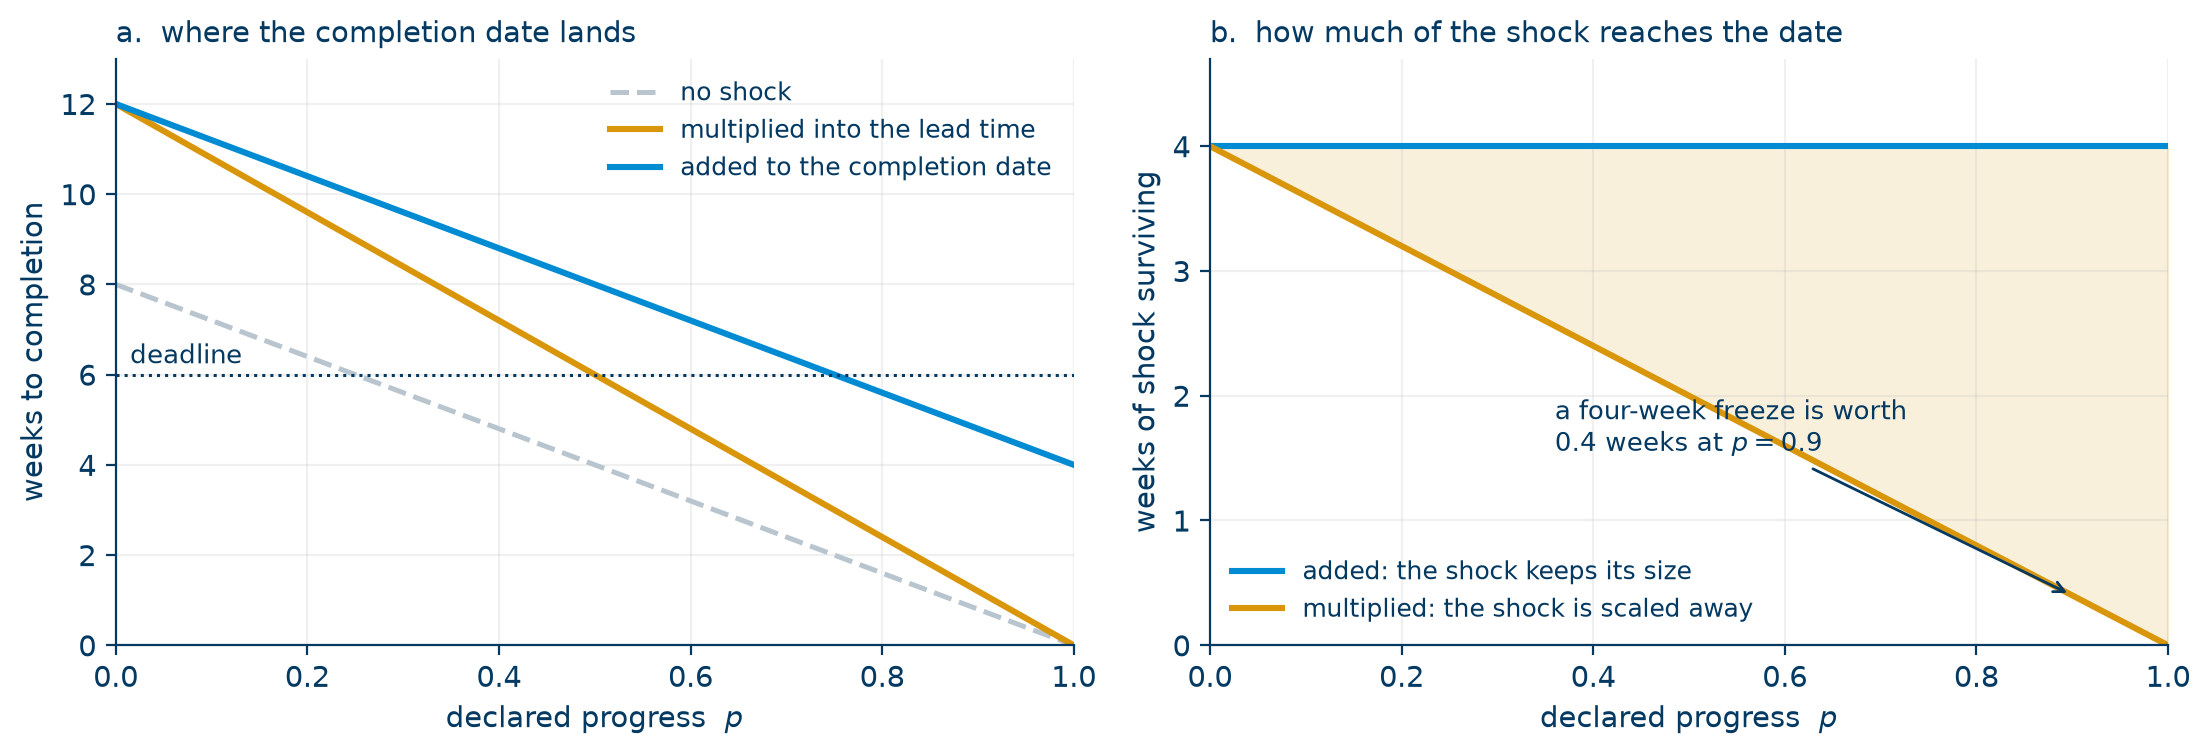
\includegraphics[width=\linewidth]{Images/completion_repair.png}
    \caption[Why the obvious repair fails]{The two repairs on one milestone, with a nominal
    lead time of eight weeks and four weeks lost to a shock. Routing the lost time through the
    lead time (ochre) scales it by the work remaining, so a four-week freeze is worth $3.6$
    weeks at a tenth complete and $0.4$ weeks at nine tenths; adding it to the completion date
    (azure) keeps its size throughout. The milestones on which the two disagree most are those
    nearest their deadline, which are precisely those on which a warning has value.}
    \label{fig:completion_repair}
\end{figure}

The completion model was rewritten accordingly, identically in the three independent
estimators the system carries for the same quantity, the analytic $u_{\text{time}}$ block, the
Monte Carlo forecast rollout and the PERT lead-time simulator:
\begin{equation}
    C \;=\; t \;+\; (1 - p)\,L \;+\; R,
    \label{eq:completion_repaired}
\end{equation}
where $p$ is the declared progress, $L$ the lead time and $R$ the time already lost. Five
families of capacity-halting event, machine failure, accident, strike weighted by the share
of workforce involved, material shortage weighted by criticality, and cyber incident, now
accumulate their effective duration into $R$. Loss of storage capacity deliberately does not,
since it removes space rather than production hours.

The mechanical effect is unambiguous. Where the accumulated-delay field was written a non-zero
value exactly zero times across the whole of arm A, after the repair NovaFab accumulates
$154.7$ engine hours at its first shock and $371.2$ over the campaign, carried in 27 of its 41
snapshots.

\subsection{Two Further Defects Exposed by the First}

With the time block responsive, a second defect became measurable. The milestone-miss
probability returned exactly $0$ or exactly $1$ in $85.0\%$ of the 120 forecasts, leaving 14
anywhere in between: a switch rather than a probability, as two declarants recorded in free
text before it was measured. The cause is that the rollout drew the lead time at random while
taking declared progress as an exact value. Declared progress is the least reliable input the
system receives and belongs to precisely the class of quantity the framework exists to doubt,
so the forecast layer was treating as certain a figure the adequacy score is built to suspect.
Progress is now drawn per replicate, with a standard deviation widened node by node in
proportion to that node's own measured hidden risk $H$, so the system's adequacy measurement
feeds its own forecast.

The third defect was in the data rather than the model, and it would have invalidated any
calibration performed before it was found. Indicator coverage on the campaign database was
$25.6\%$: 24 of the 42 indicators were empty on all eight nodes, the carbon and cost blocks
were inert everywhere, and only three of the six urgency blocks contributed. The lead time
itself was present on five nodes of eight, and the remaining three received a risk floor of
zero through the documented fallback for a missing lead time, which is an absence of data
presenting itself as a reassuring prediction. Completing the indicators from public figures
of the 2020 to 2022 shortage raised coverage to $49.1\%$ and made all six blocks active. One
model bug was undetectable until then: a per-node recovery capability, a 26-week aerospace
requalification time, was being read as production time already lost, pinning that node's
time block at $1.0$ from the first turn. An empty database conceals the errors of the model
that consumes it, which is a methodological point independent of this framework.

\subsection{The Re-measurement}

Table~\ref{tab:repair_scores} scores the recomputed forecasts against the original-commitment
definition of Section~\ref{sec:res_target_trap}, at all four horizons, on the same censored
samples of 112, 104, 96 and 90 observations. The middle column of each pair isolates the
structural repair; the right-hand column adds the progress-uncertainty term.

\begin{table}[htbp]
\centering
\caption{The frozen campaign rescored after repair, original-commitment target}
\label{tab:repair_scores}
\small
\begin{tabularx}{\linewidth}{c *{6}{>{\centering\arraybackslash}X}}
\toprule
& \multicolumn{3}{c}{\textbf{Brier skill}} & \multicolumn{3}{c}{\textbf{AUC}} \\
\cmidrule(lr){2-4}\cmidrule(lr){5-7}
\textbf{Horizon} & before & structure & + uncertainty & before & structure & + uncertainty \\
\midrule
1 week  & $-1.278$ & $-0.646$ & $-0.687$ & 0.736 & 0.793 & 0.729 \\
2 weeks & $-0.690$ & $-0.401$ & $-0.367$ & 0.636 & 0.671 & 0.634 \\
3 weeks & $-0.654$ & $-0.360$ & $-0.286$ & 0.641 & 0.657 & 0.602 \\
4 weeks & $-0.553$ & $-0.272$ & $-0.216$ & 0.654 & 0.721 & 0.584 \\
\bottomrule
\end{tabularx}
\end{table}

\begin{figure}[htbp]
    \centering
    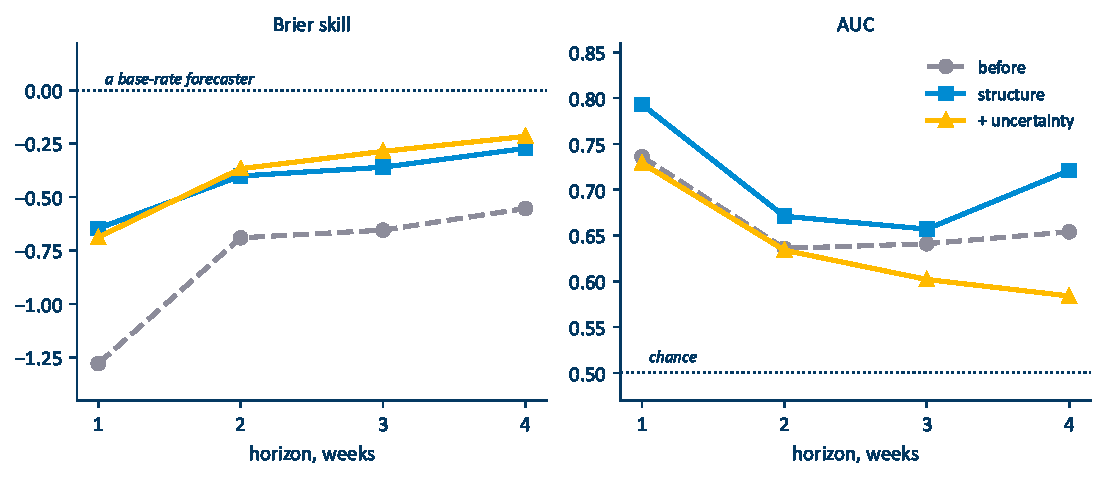
\includegraphics[width=\linewidth]{Images/repair_effect.pdf}
    \caption[What the repair bought and what it traded]{The same three model versions on both
    metrics. The structural repair lifts calibration and discrimination together. The
    progress-uncertainty term then lifts calibration further at every horizon beyond one week
    and lowers discrimination at every horizon, which is a trade rather than a gain and is why
    it was retained on the calibration evidence rather than on the AUC.}
    \label{fig:repair_effect}
\end{figure}

The structural repair improves both axes at every horizon without trading one for the other,
which is the clean result of this thesis's second measurement campaign. The
progress-uncertainty term is a trade rather than a gain, and the AUC movement it costs is not
interpretable. With 26
positive observations the cluster-bootstrap interval on the four-week AUC runs from $0.21$ to
$0.87$ and contains every value in its row, and the same objection that bounds the original
discrimination claim of Section~\ref{sec:res_armA_scored} bounds this one. The term was
retained on the calibration evidence and on the argument that a declared quantity should not
enter a probabilistic forecast as a certainty, not on the AUC.

Three qualifications belong beside the table. The Brier skill remains negative at every
horizon, so the forecast is still worse calibrated than a forecaster that announces the base
rate and stops; the repair moves the system from badly wrong to less wrong, not to useful.
The milestone probability remains binary in $71.7\%$ of cases against $85.0\%$ before, so the
over-confidence is reduced rather than removed. And the post-hoc calibration layer that
Section~\ref{sec:res_discussion} recommended was trained, measured, and deliberately not
connected: on the synthetic factory that produced its training data it improves the Brier
skill by $30.8\%$ and the AUC from $0.792$ to $0.850$, but applied to the campaign it improves
calibration at every horizon while dropping the four-week AUC from $0.721$ to $0.580$. Its
training label is an event striking the node at exactly $t+1$; the product displays a missed
milestone or a critical event cumulated over $(t, t+4]$. The layer cannot rank the cases
driven by the milestone channel because it has never seen one. This is the trap of
Section~\ref{sec:res_target_trap} encountered from the opposite direction: a calibration
fitted against the wrong target degrades a system that works, exactly as an evaluation
against the wrong target can condemn one. Connecting the layer requires the training label to
be rebuilt on the product's target, which requires the synthetic factory's snapshots to
record milestone truth, which they do not; that is the next concrete step rather than an
open research question.

\subsection{A Third Arm, and What It Does Not Show}

The repaired system was then exercised through a full nineteen-turn campaign in closed loop,
in which the same eight agents no longer only declared but also selected actions from a fixed
catalogue, applied to the chain by the mutation service and recorded in the intervention
journal: promote a backup arc, replan a milestone, expedite a shipment, raise capacity, revise
a declaration, or do nothing. One hundred and fifty-two declarations were recorded with no
unresolved consistency failure. The anti-contamination protocol of
Section~\ref{sec:methods_controls} was tightened for this arm: every message reaching an agent
is written by the tool into that agent's own sandbox, and a failed consistency check is
answered with the interface's own guidance rather than with a coordinator's instruction.

\begin{figure}[htbp]
\centering
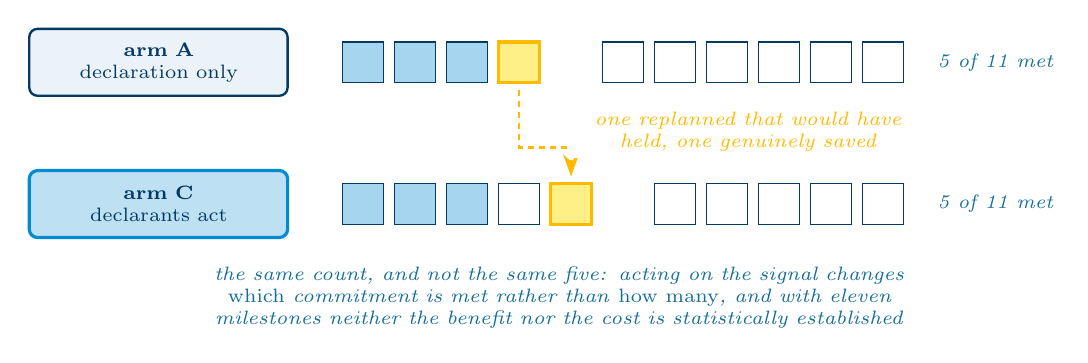
\begin{tikzpicture}[x=1cm, y=1cm, font=\scriptsize,
    arm/.style  = {bloc, text width=3.0cm, minimum height=0.85cm},
    met/.style  = {minimum width=0.52cm, minimum height=0.52cm, draw=altenNavy,
                   line width=0.5pt, fill=altenAzure!35},
    miss/.style = {minimum width=0.52cm, minimum height=0.52cm, draw=altenNavy,
                   line width=0.5pt, fill=white},
    swap/.style = {minimum width=0.52cm, minimum height=0.52cm, draw=altenOchreDark,
                   line width=1.2pt, fill=altenOchrePale}]

\node[arm] (a) at (1.9, 1.5) {\textbf{arm A}\\declaration only};
\node[arm, blocFort] (c) at (1.9, -0.3) {\textbf{arm C}\\declarants act};

%% arm A meets milestones 1..5
\foreach \i in {1,2,3,4} {
  \pgfmathsetmacro{\x}{4.5 + 0.66*(\i-1)}
  \node[met] at (\x, 1.5) {};
}
\node[swap] at (6.48, 1.5) {};                      % the one arm C replans away
\foreach \i in {6,7,8,9,10,11} {
  \pgfmathsetmacro{\x}{4.5 + 0.66*(\i-1)}
  \node[miss] at (\x, 1.5) {};
}

%% arm C keeps four, loses the fifth, gains the sixth
\foreach \i in {1,2,3,4} {
  \pgfmathsetmacro{\x}{4.5 + 0.66*(\i-1)}
  \node[met] at (\x, -0.3) {};
}
\node[miss] at (6.48, -0.3) {};
\node[swap] at (7.14, -0.3) {};                     % the one arm C saves
\foreach \i in {7,8,9,10,11} {
  \pgfmathsetmacro{\x}{4.5 + 0.66*(\i-1)}
  \node[miss] at (\x, -0.3) {};
}

\node[etiquette, anchor=west, fill=none] at (11.7, 1.5) {5 of 11 met};
\node[etiquette, anchor=west, fill=none] at (11.7, -0.3) {5 of 11 met};

\draw[flecheCoupee] (6.48, 1.15) -- (6.48, 0.42) -- (7.14, 0.42) -- (7.14, 0.05);
\node[etiquette, anchor=south, text=altenOchreDark, text width=4.4cm] at (9.4, 0.28)
     {one replanned that would have held, one genuinely saved};

\node[etiquette, anchor=north, text width=12cm] at (7.0, -1.0)
     {the same count, and not the same five: acting on the signal changes \emph{which}
      commitment is met rather than \emph{how many}, and with eleven milestones neither the
      benefit nor the cost is statistically established};

\end{tikzpicture}
\caption[The third arm changes which, not how many]{Milestones met on their original
commitment, arm~A against arm~C on the repaired system. The totals are identical and the sets
are not: the two ochre squares are the swap. That is the effect a human campaign would need
to be powered to detect.}
\label{fig:third_arm}
\end{figure}

The headline figure flatters the framework and should not be used: six of eleven milestones
were missed in the frozen scenario and none was left unfinished in the closed loop, which reads
as six saved. Against the original commitments it is not, and Figure~\ref{fig:third_arm} gives
the honest count. The saved milestone is an electronics series delivered on its original date
that had slipped in the frozen truth. Beyond the swap, four late deliveries became replannings
announced in advance rather than slips discovered at the deadline, which has value to a customer
without being a save. Both the benefit and the cost are reported as facts of one campaign rather
than as results.

Two observations from that arm do carry. The arm B disarming reproduced exactly, eight
agents of eight at first exposure. And the causal chain the campaign showed to be broken now
closes: where arm A's foundry manager recorded that the tool was holding a low position
through a widely reported crisis and took no action, the repaired run moved the same node's
four-week probability from $0.088$ to $0.214$ at the shock turn and the agent replanned its
milestone. One reserve on internal validity must be stated: the model changed twice during
that campaign, at turns 15 and 16, so turns 16 to 18 are not comparable with what precedes
them. Every behavioural observation reported above is drawn from turns strictly earlier than
15.

\subsection{A Hypothesis That Became Measurable Again}

The criticality index degenerates under saturation, which forced H3 to be judged on the ten informative turns of nineteen and the other nine to be excluded. That exclusion rule is no longer necessary. The ranking now carries a log-survival key, $\ell(p) = -\ln(1-p)$ computed on an $\varepsilon$-regularised twin of the same propagation, which orders identically to $\Delta U_r$ outside saturation, a property-based invariant with a test to match, and keeps separating nodes inside it.

Re-measured on the repaired run, the two criteria decompose cleanly on the same data. The old criterion alone leaves 10 informative turns with NovaFab top-1 on 9 of them; adding the $\Delta \ell$ key leaves 17 informative turns of 19 with NovaFab top-1 on 16, a share of $94\%$ against a pre-registered threshold of $80\%$. Holding the criterion fixed instead and changing only the model, the frozen campaign gives $70\%$ and the repaired one $90\%$, so completing the indicators moves the figure as much as the new key does.

This is reported as exploratory and does not re-decide H3, for the same reason given for H4 in Section~\ref{sec:hypothesis_status}: a hypothesis re-run against a changed model no longer tests what the register asked, and two things changed at once here. Only the comparison of the two criteria on one run isolates a single cause. The defensible claim is the narrow one: the degeneracy that made nearly half the campaign unreadable is largely gone, and the quantity H3 tests now sits above its threshold on the repaired system.


%% ═══════════════════════════════════════════════════════════════════════════


\end{document}
